\documentclass{report}

\usepackage[latin1]{inputenc}
\usepackage{enumerate}
\usepackage{a4}
\usepackage{epsfig}
\usepackage{amssymb}
\usepackage{theorem}
\usepackage{fancyvrb}
\usepackage{alltt}
\usepackage{fleqn}
\usepackage{epic}
\usepackage{color}
\usepackage{wasysym}
\usepackage{hyperref}
\usepackage[all]{hypcap}
\hypersetup{
	colorlinks = true, % comment this to make xdvi work
	linkcolor  = blue,
	citecolor  = red,
        filecolor  = blue,
        urlcolor   = [rgb]{0.5, 0.4, 0.0},
	pdfborder  = {0 0 0} 
}
\usepackage{fancyhdr}
\usepackage{lastpage} 

\renewcommand*{\familydefault}{\sfdefault}

\pagestyle{fancy}

\fancyfoot[C]{--- \thepage/\pageref{LastPage}\ ---}

\fancypagestyle{plain}{%
\fancyhf{}
\fancyfoot[C]{--- \thepage/\pageref{LastPage}\ ---}
\renewcommand{\headrulewidth}{0pt}
}

\renewcommand{\chaptermark}[1]{\markboth{\chaptername \ \thechapter.\ #1}{}}
\renewcommand{\sectionmark}[1]{\markright{\thesection. \ #1}{}}
\fancyhead[R]{\leftmark}
\fancyhead[L]{\rightmark}


\definecolor{amethyst}{rgb}{0.2, 0.4, 0.6}
\definecolor{orange}{rgb}{1, 0.9, 0.0}

\setlength{\mathindent}{1.3cm}
\theoremstyle{plain}
\newcounter{aufgabe}
\hyphenation{Warte-schlan-ge}
\hyphenation{Ko-die-rungs}
{\theorembodyfont{\sf} \newtheorem{Definition}{Definition}}
{\theorembodyfont{\sf} \newtheorem{Notation}[Definition]{Notation}}
{\theorembodyfont{\sf} \newtheorem{Corollary}[Definition]{Corollary}}
{\theorembodyfont{\sf} \newtheorem{Lemma}[Definition]{Lemma}}
{\theorembodyfont{\sf} \newtheorem{Proposition}[Definition]{Proposition}}
{\theorembodyfont{\sf} \newtheorem{Theorem}[Definition]{Theorem}}
\title{
\epsfig{file=dhbw-logo.eps, scale=1.5}\\[0.3cm]  
       Algorithms  \\[0.5cm]
      --- Lecture Notes for the Summer Term 2016 ---}
\author{Prof.~Dr.~Karl Stroetmann}

\date{\today \\[2.5cm]
\noindent
\begin{minipage}[t]{1.0\linewidth} 
These lecture notes, their \LaTeX\ sources, and the programs discussed in these lecture notes are all available at
\\[0.2cm]
\hspace*{\fill}
\href{https://github.com/karlstroetmann/Algorithms}{\texttt{https://github.com/karlstroetmann/Algorithms}}.
\hspace*{\fill} 
\\[0.2cm]
The lecture notes itself can be found in the file 
\\[0.2cm]
\hspace*{1.3cm}
\href{https://github.com/karlstroetmann/Algorithms/blob/master/Lecture-Notes/algorithms.pdf}{\texttt{Lecture-Notes/algorithm.pdf}}.
\\[0.2cm]
The lecture notes are subject to continuous change.  Provided the program \href{http://git-scm.com/download}{\texttt{git}}
is installed on your computer, the repository containing the lecture notes can be cloned using the command
\\[0.2cm]
\textcolor{amethyst}{\texttt{git clone https://github.com/karlstroetmann/Algorithms.git}}.
\\[0.2cm]
Once you have cloned the repository, the command
\\[0.2cm]
\hspace*{1.3cm}
\textcolor{amethyst}{\texttt{git pull}}
\\[0.2cm]
can be used to load the current version of these lecture notes from 
\href{https://github.com}{\texttt{github}}.
\end{minipage}
}

\newcommand{\exercise}{\vspace*{0.3cm}
\stepcounter{aufgabe}
\noindent
\textbf{Exercise \arabic{aufgabe}}: }

\newcommand{\proof}{\vspace*{0.3cm}
\noindent
\textbf{Proof}: }

\newcommand{\solution}{\vspace*{0.3cm}
\noindent
\textbf{Solution}: }

\newcommand{\example}{\vspace*{0.3cm}
\noindent
\textbf{Example}: \ }

\newcommand{\examples}{\vspace*{0.3cm}

\noindent
\textbf{Examples}: \ }

\newcommand{\remark}{\vspace*{0.3cm}

\noindent
\textbf{Remark}: \ }

\newcommand{\mod}{\;\texttt{\%}\;}
\newcommand{\hoare}[3]{\bigl\{#1\bigr\}\quad\texttt{#2}\quad\bigl\{#3\bigr\}}
\newcommand{\folge}[1]{\bigl(#1\bigr)_{n\in\mathbb{N}}}
\newcommand{\bruch}[2]{{\displaystyle \frac{\displaystyle \raisebox{1pt}[0pt][-0pt]{$\,#1\,$}}{\displaystyle \raisebox{0pt}[10pt]{$\,#2\,$}}}}
\newcommand{\h}{\mathcal{H}}
\newcommand{\Oh}{\mathcal{O}}
\newcommand{\Java}{\textsl{Java}}
\newcommand{\Bin}{\mathcal{B}}
\newcommand{\AVL}{\mathcal{A}}
\newcommand{\head}{\mbox{\tt head}}
\newcommand{\tail}{\mbox{\tt tail}}
\newcommand{\conclude}{\hspace*{\fill} $\Box$}
\newcommand{\nodes}{{\mathbb V}}
\newcommand{\edges}{{\mathbb E}}
\newcommand{\paths}{{\mathbb P}}
\newcommand{\weight}[1]{\|#1\|}
\newcommand{\Weight}[1]{\bigl\|#1\bigr\|}
\newcommand{\N}{{\mathbb N}}
\newcommand{\R}{{\mathbb R}}
\newcommand{\df}{\;:=\;}
\newcommand{\ds}{\displaystyle}
\newcommand{\source}{\mbox{\tt source}}
\newcommand{\target}{\mbox{\tt target}}
\newcommand{\spath}{\mbox{\tt sp}}
\newcommand{\el}{\!\in\!}
\newcommand{\BT}{\mathrm{BT}}
\def\pair(#1,#2){\langle #1, #2 \rangle}
\newcommand{\qed}{\hspace*{\fill} $\Box$}
\newcommand{\eox}{\hspace*{\fill} $\diamond$}
\newcommand{\lb}{\hspace*{\fill} \linebreak}

\hyphenation{stra-te-gy}

\begin{document}
\maketitle
\tableofcontents
\chapter{Introduction}
\section{Motivation}
The previous lecture in the winter term has shown us how interesting problems can be solved with the
help of sets and relations.  However, we did not discuss how sets and relations can be represented
and how the operations on sets can be implemented in an efficient way.  This course will answer
these questions:  We will see data structure that can be used to represent sets in an efficient way.
Furthermore, we will discuss a number of other data structures and algorithms that should be in the
toolbox of every computer scientist.

While the class in the last term has introduced the students to the theoretical foundations of
computer science, this class is more application oriented.  Indeed, it may be one of the most 
important classes for your future career: Stanford University regularly asks their former students 
to rank those classes that were the most useful for their professional career.  Together with
programming and databases, the class on algorithms consistently ranks highest.  The practical
importance of the topic of this class can also be seen by the availability of book titles like 
 ``Algorithms for Interviews'' \cite{aziz:10} or the
\href{http://www.youtube.com/watch?v=k4RRi_ntQc8}{Google job interview questions}.
 
 
\section{Overview}
This lecture covers the design and the analysis of algorithms.  We will discuss the following topics.
\begin{enumerate}
\item Undecidability of the \href{http://en.wikipedia.org/wiki/Halting_problem}{halting problem}.

      At the beginning of the lecture we discuss the limits of computability:  We will show that
      there is no \textsc{SetlX} function \texttt{doesTerminate} such that for a given function $f$
      of one argument and a string $s$ the expression
      \\[0.2cm]
      \hspace*{1.3cm}
      $\texttt{doesTerminate}(f, s)$ 
      \\[0.2cm]
      yields \texttt{true} if the evaluation of $f(s)$ terminates and yields \texttt{false} otherwise.
\item \href{http://en.wikipedia.org/wiki/Computational_complexity_theory}{Complexity} of algorithms.

      In general, in order to solve a given problem it is not enough to develop an algorithm that
      implements a function $f$ that computes values $f(x)$ for some argument $x$.  If the size of
      the argument $x$ is big, then it is also important  
      that the computation of $f(x)$ does not take too much time.  Therefore, we want to have
      \emph{efficient} algorithms.
      In order to be able to discuss the efficiency of algorithms we have to introduce two 
      mathematical notions.
      \begin{enumerate}
      \item \href{http://en.wikipedia.org/wiki/Recurrence_relation}{\emph{Recurrence relations}}
            are discrete analogues of differential equations.  Recurrence relations occur naturally
            when analyzing the runtime of algorithms.
      \item \href{http://en.wikipedia.org/wiki/Big_Oh}{\emph{Big O notation}} offers a convenient way to
            discuss the growth rate of functions.  This notation is useful to abstract from
            unimportant details when discussing the runtime of algorithms.  
      \end{enumerate}
\item \href{http://en.wikipedia.org/wiki/Abstract_data_types}{Abstract data types}.

      Abstract data types are a means to describe the behavior of an algorithm in a concise way.
\item \href{http://en.wikipedia.org/wiki/Sorting_algorithm}{Sorting algorithms}.

      Sorting algorithm are the algorithms that are most frequently used in practice.  As these
      algorithms are, furthermore, quite easy to understand they serve best for an introduction to
      the design of algorithms.  We discuss the following sorting algorithms:
      \begin{enumerate}
      \item \href{http://en.wikipedia.org/wiki/Insertion_sort}{insertion sort},
      \item \href{http://en.wikipedia.org/wiki/Selection_sort}{selection sort},
      \item \href{http://en.wikipedia.org/wiki/Merge_sort}{merge sort}, and
      \item \href{http://en.wikipedia.org/wiki/Quicksort}{quicksort}.
      \end{enumerate}
\item \href{http://en.wikipedia.org/wiki/Hoare_logic}{Hoare logic}.
  
      The most important property of an algorithm is its correctness.  The \emph{Hoare calculus}
      is a method to investigate the correctness of an algorithm.  

\item \href{http://en.wikipedia.org/wiki/Map_(computer_science)}{Associative arrays}.
  
      Associative arrays are a means to represent a function.  We discuss
      various data structures that can be used to implement associative arrays efficiently.
\item \href{http://en.wikipedia.org/wiki/Priority_queue}{Priority queues}.
  
      Many graph theoretical algorithms use priority queues as a basic building block.
      Furthermore, priority queues have important applications in the theory of operating systems
      and in simulation.
\item \href{http://en.wikipedia.org/wiki/Graph_theory}{Graph theory}.
  
      There are many applications of graphs in computer science.  The topic of graph theory is very
      rich and can easily fill a class of its own.  Therefore, we can only cover a small subset of this topic.
      In particular, we will discuss
      \href{http://en.wikipedia.org/wiki/Dijkstra%27s_algorithm}{Dijkstra's algorithm}
      for computing the shortest path.
\item \href{http://en.wikipedia.org/wiki/Monte_Carlo_method}{Monte Carlo Method} 
 
      Many important problems either do not have an exact solution at all or the computation of an
      exact solution would be prohibitively expensive.  In these cases it is often possible to use 
      simulation in order to get an approximate solution.  As a concrete example we will show
      how certain probabilities in \href{http://en.wikipedia.org/wiki/Texas_hold_%27em}{Texas hold 'em} 
      poker can be determined approximately with the help of the Monte
      Carlo method.
\end{enumerate}
The primary goal of these lectures on algorithms is not to teach as many algorithms as possible.
Instead, I want to teach how to think algorithmically:  At the end of these
lectures, you should be able to develop your own algorithms on yourself.  This is a process that
requires a lot of creativity on your side, as there are no cookbook recipes that can be followed.
However, once you are acquainted with a fair number of algorithms, you should be able to discover
algorithms on your own.

\section{Algorithms and Programs}
This is a lecture on algorithms, not on programming.  It is important that you do not mix up
programs and algorithms.  An algorithm is an \emph{abstract} concept to solve a given problem.  In
contrast, a program is a \emph{concrete} implementation of an algorithm.  In order to implement an
algorithm by a program we have to cover every detail, be it trivial or not.  On the other hand, 
to specify an algorithm it is often sufficient to describe the interesting aspects.  It is
quite possible for an algorithm to leave a number of questions open.

In the literature, algorithms are mostly presented as pseudo code.  Syntactically, pseudo code looks
similar to a program, but in contrast to a program, pseudo code can also contain parts that are only
described in natural language.   However, it is important to realize that a piece of pseudo code is
\underline{not} an algorithm but is only a \emph{ representation} of an algorithm.  However, the
advantage of pseudo code is that we are not confined by the randomness of the syntax of a
programming language.

Conceptually, the difference between an algorithm and a program is similar to the difference between
an \emph{idea} and a \emph{text} that describes the idea.  If you have an idea, you can write it down to
make it concrete.  As you can write down the idea in English or French or any other language, the
textual descriptions of the idea might be quite different.  This is the same with an algorithm:  We
can code it in \textsl{Java} or \textsc{Cobol} or any other language.  The programs will be very
different but the algorithm will be the same.

Having discussed the difference between algorithms and programs, let us now decide how to present
algorithms in this lecture.  
\begin{enumerate}
\item We can describe algorithms using natural language.  While natural language certainly is
      expressive enough, it also suffers from ambiguities.  Furthermore, natural language
      descriptions of complex algorithms tend to be very hard to understand.
\item Instead, we can describe an algorithm by implementing it.  There is certainly no ambiguity
      in a program, but on the other hand this approach would require us to implement every aspect
      of an  algorithm and our descriptions of algorithms would therefore get longer than we want.
\item Finally, we can try to describe algorithms in the language of mathematics.  This language is 
      concise, unambiguous, and easy to understand, once you are accustomed to it.  This is
      therefore our method of choice.

      However, after having presented an algorithm in the language of mathematics, it is often very
      simple to implement this algorithm in the programming language
      \href{http://randoom.org/Software/SetlX}{\textsc{SetlX}}.  The reason is 
      that \textsc{SetlX} is based on set theory, which is the language of mathematics.  We will see
      that \textsc{SetlX} enables us to present and implement algorithms on a very high abstraction level.
\end{enumerate}

\section{Desirable Properties of Algorithms}
Before we start with our discussion of algorithms we should think about our goals when designing
algorithms.  
\begin{enumerate}
\item Algorithms have to be \emph{correct}.
\item Algorithms should be as \emph{efficient} as possible.
\item Algorithms should be \emph{simple}.
\end{enumerate}
The first goal in this list is so self-evident that it is often overlooked.  The
importance of the last goal might not be as obvious as the other goals.
However, the reasons for the last goal are economical:  If it takes too long to code an algorithm, the
cost of the implementation might well be unaffordable.  Furthermore, even if the budget is unlimited there 
is another reasons to strife for simple algorithms:
If the conceptual complexity of an algorithm is too high, it may become impossible to check
the correctness of the implementation.  Therefore, the third goal is strongly related to the first
goal.  

\section{Literature}
These lecture notes are available online at
\\[0.2cm]
\hspace*{1.3cm}
\href{https://github.com/karlstroetmann/Algorithms/blob/master/English-Script/algorithms.pdf}{https://github.com/karlstroetmann/Algorithms/blob/master/English-Script/algorithms.pdf}.  
\\[0.2cm]
They are intended to be the main source for my lecture.  Additionally, I want
to mention those books that have inspired me most.
\begin{enumerate}
\item \textsl{Alfred V.~Aho}, \textsl{John E.~Hopcraft}, and \textsl{Jeffrey D.~Ullman}:
      \emph{Data Structures and Algorithms}, Addison-Wesley, 1987, \cite{aho:87}.
      
      This book is quite dated now but it is one of the classics on algorithms.  It discusses algorithms at an
      advanced level.
\item \textsl{Thomas H.~Cormen}, \textsl{Charles E.~Leiserson}, 
      \textsl{Ronald L.~Rivest}, and \textsl{Clifford Stein}:
      \emph{Introduction to Algorithms}, 
      third edition, MIT Press, 2009, \cite{cormen:09}

      Due to the level of detail and the number of algorithms given, this book is well suited as a
      lookup library.
\item \textsl{Robert Sedgewick}: \emph{Algorithms in \textsl{Java}}, 
      fourth edition, Pearson, 2011, \cite{sedgewick:11}.
    
      This book has a nice \href{http://algs4.cs.princeton.edu/home/}{booksite} containing a wealth
      of additional material.  This book seems to be the best choice for the working practitioner.
      Furthermore, \href{http://www.cs.princeton.edu/~rs/}{Professor Sedgewick} teaches a 
      \href{https://www.coursera.org/course/algs4partI}{course} on algorithms on 
      \href{https://www.coursera.org/}{coursera} that is based on this book.
\item \emph{Einf�hrung in die Informatik},
      written by \textsl{Heinz-Peter Gumm} and \texttt{Manfred Sommer} \cite{gumm:2008}.
      
      This German book is a very readable introduction to computer science and it has a comprehensive chapter
      on algorithms.  Furthermore, this book is
      \href{http://www.oldenbourg-link.com/doi/book/10.1524/9783486595390}{available} electronically
      in our library. 
\item Furthermore, there is a set of 
      \href{https://class.coursera.org/algo-003/class/index}{video lectures} 
      from \href{http://theory.stanford.edu/~tim/}{Professor Roughgarden}
      at \href{https://www.coursera.org/}{coursera}.
\item \href{http://www.cs.berkeley.edu/~vazirani/algorithms/all.pdf}{\emph{Algorithms}},
      written by \textsl{Sanjoy Dasgupta, Christos H.~Papadimitriou, and Unmesh V.~Vazirani} \cite{dasgupta:2008}
      is a short text book on Algorithms that is available online.
\item \href{http://www.mpi-inf.mpg.de/~mehlhorn/Toolbox.html}{\emph{Data Structures and Algorithms}}
      written by \emph{Kurt Mehlhorn and Peter Sanders} \cite{mehlhorn:2008} is another good text
      book on algorithms that is available online.
\end{enumerate}


\section{A Final Remark}
There is one final remark I would like to make at this point:  Frequently, I get questions from
students concerning the exams.  While I will answer most of them, I should warn you that, 50\% 
of the time, my answers will be lies.  The other 50\%,
my answers will be either dirty lies or accidentally true.

\section{A Request}
Computer science is a very active field of research.  Therefore, these lecture notes are constantly
evolving and hence might contain typos or bugs.  If you find a bug, please take the time and send me
an email.  My email address is
\\[0.2cm]
\hspace*{1.3cm}
\href{mailto:karl. stroetmann@ dhbw- mannheim. de}{karl.stroetmann@dhbw-mannheim.de}.
\\[0.2cm]
If you are familiar with \href{http://github.com}{\texttt{github}}, you might even consider
sending me a \href{https://help.github.com/articles/using-pull-requests}{pull request}.


%%% local Variables: 
%%% mode: latex
%%% TeX-master: "algorithms"
%%% End: 

%\chapter{Limits of Computability}
Every discipline of the sciences has its limits: Students of the medical sciences soon realize that
it is difficult to \href{http://www.wowhead.com/spell=61999}{raise the dead}, while
adepts of theology have to admit that there is no way they 
can \href{http://www.youtube.com/watch?v=RUMX_b_m3Js}{walk on water}.  But believe it or not, even
computer science has its limits!  We will discuss 
these limits next.  First, we show that we cannot decide whether a computer program will eventually
terminate or whether it will run forever.  
Second, we prove that it is impossible to check whether two programs are equivalent.


\section{The Halting Problem}
In this subsection we prove that it is not possible for a computer program to decide whether 
another computer program does terminate.  This problem is known as the 
\href{http://en.wikipedia.org/wiki/Halting_problem}{\emph{halting problem}}.
Before we give a formal proof that the halting problem is undecidable, let us
discuss one example that shows why it is indeed difficult to decide whether a program does always
terminate.  Consider the program shown in Figure \ref{fig:legendre.stlx} on page
\pageref{fig:legendre.stlx}.  This program contains an obvious infinite loop in line 6.   However,
this loop is only entered if the expression
\\[0.2cm]
\hspace*{1.3cm}
$\mathtt{legendre}(n)$
\\[0.2cm]
in line 5 evaluates to \texttt{false}.  Given a natural number \texttt{n}, the expression
$\texttt{legendre}(n)$ tests whether there is a prime between $\texttt{n}^2$ and $(\texttt{n}+1)^2$.  
If, however, the intervall
\\[0.2cm]
\hspace*{1.3cm}
$[n^2, (n+1)^2] := \{ k \in \mathbb{N} \mid n^2 \leq k \wedge k \leq (n+1)^2 \}$
\\[0.2cm]
does not contain a prime number, then $\texttt{legendre}(n)$ evaluates
to \texttt{false} for this value of $n$.  The function \texttt{legendre} is defined in line 2.  
Given a natural number $n$, it returns \texttt{true} if and only if the formula
\\[0.2cm]
\hspace*{1.3cm}
$\exists k \in \mathbb{N}: n^2 \leq k \wedge k \leq (n+1)^2 \wedge \textsl{isPrime}(k)$
\\[0.2cm]
holds true.  The French mathematican 
\href{http://en.wikipedia.org/wiki/Adrien-Marie_Legendre}{Adrien-Marie Legendre} (1752 -- 1833) conjectured that
for any natural number $n \in \mathbb{N}$ there is prime number $p$ such that
\\[0.2cm]
\hspace*{1.3cm}
$n^2 \leq p \wedge  p \leq (n+1)^2$
\\[0.2cm]
holds.  Although there are a number of reasons in support of Legendre's conjecture,  to this day
nobody has been able to prove it.  The question, whether the invocation of the function $f$ will
terminate for every user input is, therefore, unknown as it depends on the truth of 
\href{http://en.wikipedia.org/wiki/Legendre's_conjecture}{Legendre's conjecture}:  If we
had some procedure that could check whether the function \texttt{main} does terminate for every number
$n$ that is input by the user,
then this procedure would be able to decide whether Legendre's theorem is true.  Therefore, it
should come as no surprise that such a procedure does not exist.


\begin{figure}[!ht]
\centering
\begin{Verbatim}[ frame         = lines, 
                  framesep      = 0.3cm, 
                  firstnumber   = 1,
                  labelposition = bottomline,
                  numbers       = left,
                  numbersep     = -0.2cm,
                  xleftmargin   = 0.0cm,
                  xrightmargin  = 0.0cm,
                ]
    main := procedure() {
        legendre := n |-> exists (k in [n**2..(n+1)**2] | isPrime(k));

        n := read("input a natural number: ");
        if (!legendre(n)) {
            while (true) {
                print("looping");
            } 
        }
        return true;
    };
\end{Verbatim}
\vspace*{-0.3cm}
\caption{A program running into trouble if Legendre's was wrong.}
\label{fig:legendre.stlx}
\end{figure}

Let us proceed to prove formally that the halting problem is not solvable.  To this end, we need the
following definition.

\begin{Definition}[Test Function] 
A string $t$ is a \emph{test function with name $n$} iff $t$ has the form 
\\[0.2cm]
\hspace*{1.3cm} 
\texttt{$n$ := procedure(x) \{ $\cdots$ \};}
\\[0.2cm]
and, furthermore, the string $t$ can be parsed as a \textsc{SetlX} statement, that is the evaluation of
the expression
\\[0.2cm]
\hspace*{1.3cm}
\texttt{parseStatements(t);}
\\[0.2cm]
does not yield an error.  
The set of all test functions is denoted as $T\!F$.  If $t \in T\!F$ and $t$ has the name $n$, then
this is written as 
\\[0.2cm]
\hspace*{1.3cm}
$\mathtt{name}(t) = n$. \hspace*{\fill} $\Box$
\end{Definition}

\examples
\begin{enumerate}
\item $s_1$ = ``{\tt simple := procedure(x) \{ return 0; \};}''

      $s_1$ is a test function with the name \texttt{simple}.
\item $s_2$ = ``{\tt loop := procedure(x) \{ while (true) \{ x := x + 1; \} \};}''

      $s_2$ is a test function with the name \texttt{loop}. 
\item $s_3$ = ``{\tt hugo := procedure(x) \{ return ++x; \};}''

      $s_3$ is not a test function.  The reason is that \textsc{SetlX} does not support the operator
      ``\texttt{++}''.  Therefore, 
      \\[0.2cm]
      \hspace*{1.3cm}
      \texttt{parseStatements(s3)}
      \\[0.2cm]
      yields an error message complaining about the two ``\texttt{+}'' characters.
\end{enumerate}
In order to be able to formalize the halting problem succinctly, we introduce three additional
notations.

\begin{Notation}[$\leadsto$, $\downarrow$, $\uparrow$]
If $n$ is the name of a \textsc{SetlX} function that takes $k$ arguments $a_1$, $\cdots$, $a_k$,
then we write 
\\[0.2cm]
\hspace*{1.3cm}
 $n(a_1, \cdots, a_k) \leadsto r$ 
\\[0.2cm]
iff the evaluation of the expression $n(a_1, \cdots, a_k)$ yields the result $r$.  If we are not
concerned with the result $r$ but only want to state that the evaluation terminates,
then we will write
\\[0.2cm]
\hspace*{1.3cm} $n(a_1, \cdots, a_k) \,\downarrow$ \\[0.3cm]
and read this notation as ``\emph{evaluating $n(a_1, \cdots, a_k)$ terminates}''.
If the evaluation of the expression $n(a_1, \cdots, a_k)$ does \underline{not} terminate, this is
written as \\[0.2cm]
\hspace*{1.3cm}
 $n(a_1, \cdots, a_k) \,\uparrow$. 
\\[0.2cm]
This notation is read as ``\emph{evaluation of $n(a_1, \cdots, a_k)$ diverges}''.
\hspace*{\fill} $\Box$
\end{Notation}

\examples  Using the test functions defined earlier, we have:
\begin{enumerate}
\item {\tt simple(\symbol{34}emil\symbol{34}) $\leadsto 0$},
\item {\tt simple(\symbol{34}emil\symbol{34}) $\downarrow$},
\item {\tt loop(2) $\uparrow$}.
\end{enumerate}

\noindent
The \emph{halting problem} for \textsc{SetlX} functions is the question whether there is a
\texttt{SetlX} function \\[0.2cm]
\hspace*{1.3cm} 
\texttt{stops := procedure($t$,$\;a$) \{ $\cdots$ \};} 
\\[0.2cm]
that takes as input a test function $t$ and a string $a$ and that satisfies the following specification:
\begin{enumerate}
\item $t \not\in T\!F \quad\Leftrightarrow\quad \mathtt{stops}(t, a) \leadsto 2$.

      If the first argument of \texttt{stops} is not a test function, then 
      \texttt{stops($t$, $a$)} returns the number $2$.

\item $t \in T\!F \,\wedge\, \mathtt{name}(t) = n \,\wedge\, n(a)\downarrow \quad\Leftrightarrow\quad
       \mathtt{stops}(t, a) \leadsto 1$.

      If the first argument of \texttt{stops} is a test function and, furthermore,
      the evaluation of $n(a)$ terminates, then \texttt{stops($t$, $a$)} returns the number $1$.

\item $t \in T\!F \,\wedge\, \mathtt{name}(t) = n \,\wedge\, n(a)\uparrow \quad\Leftrightarrow\quad
       \mathtt{stops}(t, a) \leadsto 0$.

      If the first argument of \texttt{stops} is a test function but the evaluation of $n(a)$ 
      diverges, then \texttt{stops($t$, $a$)} returns the number $0$.
\end{enumerate}
If there was a \textsc{SetlX} function \texttt{stops} that did satisfy the specification given above,
then the halting problem for \textsc{SetlX} would be decidable.

\begin{Theorem}[\href{http://en.wikipedia.org/wiki/Alan_Turing}{Alan Turing}, 1936]
  The halting problem is undecidable.
\end{Theorem}

\noindent
\textbf{Proof}:  In order to prove the undecidabilty of the halting problem we have to show that
there can be no function \texttt{stops} satisfying the specification given above.  This calls for an
indirect proof also known as \href{http://en.wikipedia.org/wiki/Indirect_proof}{\emph{proof by contradiction}}.
We will therefore assume that a function \texttt{stops} solving the halting problem does
exist and we will then show that this assumption leads to a contradiction.  This contradiction will
leave us with the conclusion that there can be no function \texttt{stops} that satisfies
the specification given above and that, therefore, the halting problem is not solvable.

In order to proceed, let us assume that a \textsc{SetlX} function \texttt{stops}
satisfying the specification given above exists and let us define the string
\textsl{turing} as shown in Figure \ref{fig:turing-string} below.

\begin{figure}[!h]
  \centering
\begin{Verbatim}[ frame         = lines, 
                  framesep      = 0.3cm, 
                  labelposition = bottomline,
                  numbers       = left,
                  numbersep     = -0.2cm,
                  xleftmargin   = 0.8cm,
                  xrightmargin  = 0.8cm,
                  commandchars  = \\\{\},
                ]
    \textsl{turing} := "alan := procedure(x) \{
                   result := stops(x, x);
                   if (result == 1) \{
                       while (true) \{
                           print(\symbol{92}"... looping ...\symbol{92}");
                       \}
                   \}
                   return result;
               \};";
\end{Verbatim}
  \vspace*{-0.3cm}
  \caption{Definition of the string \textsl{turing}.}
  \label{fig:turing-string}
\end{figure}

Given this definition it is easy to check that \textsl{turing} is, indeed, a test function with the name
``\texttt{alan}', that is we have 
\\[0.3cm]
\hspace*{1.3cm} 
$\textsl{turing} \in T\!F \;\wedge\; \mathtt{name}(\textsl{turing}) = \mathtt{alan}$. 
\\[0.2cm]
Therefore, we can use the string \textsl{turing} as the first argument of the function
\texttt{stops}.  Let us think about the following expression:
\\[0.2cm]
\hspace*{1.3cm} 
\texttt{stops(\textsl{turing}, \textsl{turing});} 
\\[0.2cm]
Since we have already noted that \textsl{turing} is test function, according to the specification of
the function \texttt{stops} there are only two cases left:
\\[0.2cm]
\hspace*{1.3cm} 
$\mathtt{stops}(\textsl{turing}, \textsl{turing}) \leadsto 0 \quad \vee\quad
 \mathtt{stops}(\textsl{turing}, \textsl{turing}) \leadsto 1$. 
\\[0.2cm]
Let us consider these cases in turn.
\begin{enumerate}
\item $\mathtt{stops}(\textsl{turing}, \textsl{turing}) \leadsto 0$. 

      According to the specification of \texttt{stops} we should then have
      \\[0.2cm]
      \hspace*{1.3cm}
      $\mathtt{alan}(\textsl{turing}) \uparrow$.
      \\[0.2cm]
      Let us check whether this is true.  In order to do this, we have to check what happens when
      the expression
      \\[0.2cm]
      \hspace*{1.3cm}
      \texttt{alan(\textsl{turing})} 
      \\[0.2cm]
      is evaluated:
      \begin{enumerate}
      \item Since we have assumed for this case that the expression 
            $\mathtt{stops}(\textsl{turing}, \textsl{turing})$ yields $0$, 
            in line 2, the variable \texttt{result} is assigned the value 0. 
      \item Line 3 now tests whether \texttt{result} is $1$.  Of course,
            this test fails.  Therefore, the block of the \texttt{if}-statement is not executed.
      \item Finally, in line 8 the value of the variable \texttt{result} is returned. 
      \end{enumerate}
      All in all we see that the call of the function \texttt{alan} does terminate with the argument
      \textsl{turing}.  However, this is the opposite of what the function \texttt{stops} has claimed.
      
      Therefore, this case has lead us to a contradiction.
\item  $\mathtt{stops}(\textsl{turing}, \textsl{turing}) \leadsto 1$. 

      According to the specification of \texttt{stops} we should then have
      \\[0.2cm]
      \hspace*{1.3cm}
      $\mathtt{alan}(\textsl{turing}) \downarrow$, 
      \\[0.2cm]
      i.e.~the evaluation of $\mathtt{alan}(\textsl{turing}) \downarrow$ should terminate.
      
      Again, let us check in detail whether this is true.  
      \begin{enumerate}
      \item Since we have assumed for this case that the expression 
            $\mathtt{stops}(\textsl{turing}, \textsl{turing})$ yields $1$, 
            in line 2, the variable \texttt{result} is assigned the value $1$. 
      \item Line 3 now tests whether \texttt{result} is $1$.  Of course,
            this time the test succeeds.  
            Therefore, the block of the \texttt{if}-statement \underline{is} executed.
      \item However, this block contains an obvious infinite loop.  Therefore, the
            evaluation of $\mathtt{alan}(\textsl{turing})$ \underline{diver}g\underline{es}.
            But this contradicts the specification of \texttt{stops}!
      \end{enumerate}   
      Therefore, the second case also leads to a contradiction.
\end{enumerate}
As we have obtained contradictions in both cases, the assumption that there is a function
\texttt{stops} that solves the halting problem is refuted.
\hspace*{\fill} $\Box$
\vspace*{0.3cm}

\noindent
\textbf{Remark}:
The proof of the fact that the halting problem is undecidable was given 1936 by Alan Turing (1912 -- 1954)
\cite{turing:36}.  Of course, Turing did not solve the problem for \textsc{SetlX} but rather
for the so called 
\href{http://en.wikipedia.org/wiki/Indirect_proof}{\emph{Turing machines}}.  
A \emph{Turing maschine} can be interpreted as a formal description of an algorithm.  
Therefore, Turing has shown, that there is no algorithm that is able to decide whether some given
algorithm will always terminate.
\vspace*{0.3cm}

\noindent
\textbf{Remark}:
Having read this far you might wonder whether there might be another programming language
that is more powerful so that programming in this more powerful language it would be possible to
solve the halting problem.  However, if you check the proof given for \textsc{SetlX} you will easily
see that this proof can be adapted to any other programming language that is as least as powerful as
\textsc{SetlX}. 

Of course, if a programming language is very restricted, then it might be possible to check the
halting problem for this weak programming language.  But for any programming language that supports
at least \texttt{while}-loops, \texttt{if}-statements, and the definition of procedures the argument
given above shows that the halting problem is not solvable.

\exercise
Show that if the halting problem would be solvable, then it would be possible to write a program that checks
whether there are infinitely many \emph{twin primes}.  A \emph{twin prime} is pair of natural numbers
$\langle p, p + 2 \rangle$ such that both $p$ and $p+2$ are prime numbers.  
The \href{http://en.wikipedia.org/wiki/Twin_prime_conjecture}{\emph{twin prime conjecture}} is one
of the oldest unsolved mathematical problems.

\exercise
A set $X$ is called \emph{countable}  iff there is a function 
\\[0.2cm]
\hspace*{1.3cm}
 $f: \mathbb{N} \rightarrow X$ 
\\[0.2cm]
such that for all $x\in X$ there is a $n \in \mathbb{N}$ such that $x$ is the image of
$n$ under $f$: 
\\[0.2cm]
\hspace*{1.3cm} $\forall x \in X: \exists n \in \mathbb{N}: x = f(n)$.
\\[0.2cm]
Prove that the set $2^\mathbb{N}$, which is the set of all subsets of $\mathbb{N}$ is \underline{not} countable. 

\vspace*{0.2cm}

\noindent
\textbf{Hint}:  Your proof should be similar to the proof that the halting problem is undecidable. 
Proceed as follows:
Assume that there is a function $f$ enumerating the subsets of $\mathbb{N}$, that is assume that 
\\[0.2cm]
\hspace*{1.3cm}
$\forall x \in 2^\mathbb{N}: \exists n \in \mathbb{N}: x = f(n)$
\\[0.2cm]
holds.  Next, and this is the crucial step, define a set \texttt{Cantor} as follows:
\\[0.2cm]
\hspace*{1.3cm} $\mathtt{Cantor} := \bigl\{ n \in \mathbb{N} \mid n \notin f(n) \bigr\}$.
\\[0.2cm]
Now try to derive a contradiction.  



\section[The Equivalence Problem]{Undecidability of the Equivalence Problem}
Unfortunately, the halting problem is not the only undecidable problem in computer science.  Another
important problem that is undecidable is the question whether two given functions always compute the
same result.  To state this more formally, we need the following definition.


\begin{Definition}[$\simeq$] 
Assume $n_1$ and $n_2$ are the names of two \textsc{SetlX} functions that take arguments
  $a_1$, $\cdots$, $a_k$.  Let us define \\[0.2cm]
\hspace*{1.3cm} 
$n_1(a_1,\cdots,a_k) \simeq n_2(a_1,\cdots,a_k)$ 
\\[0.2cm]
if and only if either of the following cases is true:
\begin{enumerate}
\item $n_1(a_1,\cdots,a_k)\uparrow \quad\wedge\quad n_2(a_1,\cdots,a_k)\uparrow$,

      that is both function calls diverge.
\item $\exists r: \Bigl(n_1(a_1,\cdots,a_k) \leadsto r \quad\wedge\quad n_2(a_1,\cdots,a_k) \leadsto
  r\Bigr)$

      that is both function calls terminate and compute the same result.
\end{enumerate}
If $n_1(a_1,\cdots,a_k) \simeq n_2(a_1,\cdots,a_k)$ holds, then the expressions $n_1(a_1,\cdots,a_k)$ and $n_2(a_1,\cdots,a_k)$ are called
\emph{partially equivalent}. \hspace*{\fill} $\Box$
\end{Definition}

\noindent
We are now ready to state the \emph{equivalence problem}.  A \textsc{SetlX} function \texttt{equal} solves the
\emph{equivalence problem} if it is defined as
\\[0.2cm]
\hspace*{1.3cm}
$\texttt{equal := procedure(p1, p2, a) \{ ... \};}$
\\[0.2cm]
and, furthermore, satisfies the following specification:
\begin{enumerate}
\item $p_1 \not\in T\!F \;\vee\; p_2 \not\in T\!F \quad\Leftrightarrow\quad \mathtt{equal}(p_1, p_2, a) \leadsto 2$.
\item If 
      \begin{enumerate}
      \item $p_1 \in T\!F \;\wedge\; \mathtt{name}(p_1) = n_1$,
      \item $p_2 \in T\!F \;\wedge\; \mathtt{name}(p_2) = n_2$ \quad and
      \item $n_1(a) \simeq n_2(a)$
      \end{enumerate}
      holds, then we must have: 
      \\[0.2cm]
      \hspace*{1.3cm} 
      $\mathtt{equal}(p_1, p_2, a) \leadsto 1$.
\item Otherwise we must have \\[0.2cm]
      \hspace*{1.3cm} 
      $\mathtt{equal}(p_1, p_2, a) \leadsto 0$.
\end{enumerate}


\begin{Theorem}[\href{http://en.wikipedia.org/wiki/Henry_Gordon_Rice}{Henry Gordon Rice}, 1953]
\hspace*{\fill} \linebreak
The equivalence problem is undecidable.  
\end{Theorem}

\noindent
\textbf{Proof}:
The proof is by contradiction.  Therefore, assume that there is a function \texttt{equal}
such that \texttt{equal} solves the equivalence problem.  Assuming \texttt{equal} exists, we will
then proceed to define a function \texttt{stops} that does solve the halting problem.
Figure \ref{fig:stops} shows how we construct the function \texttt{stops} that makes use 
of the function \texttt{equal}.



\begin{figure}[!h]
  \centering
\begin{Verbatim}[ frame         = lines, 
                  framesep      = 0.3cm, 
                  labelposition = bottomline,
                  numbers       = left,
                  numbersep     = -0.2cm,
                  xleftmargin   = 0.3cm,
                  xrightmargin  = 0.3cm
                ]
     stops := procedure(p, a) {
         f := "loop := procedure(x) { while (true) {} };";                 
         e := equal(f, p, a);
         if (e == 2) {
             return 2;
         } else {
             return 1 - e;
         }
     }
\end{Verbatim}
  \vspace*{-0.3cm}
  \caption{An implementation of the function \texttt{stops}.}
  \label{fig:stops}
\end{figure}

Notice that in line 2 the function \texttt{equal} is called with a string that is test function with
name \texttt{loop}.  This test function has the following form:
\begin{verbatim}
      loop := procedure(x) { while (true) {} };
\end{verbatim}
Obviously, the function \texttt{loop} does never terminate.
Therefore, if the argument $p$ of \texttt{stops} is a test function with name $n$, 
the function \texttt{equal} will return $1$ if $n(a)$ diverges, and will return $0$ otherwise.
But this implementation of \texttt{stops} would then solve the halting problem as
for a given test function $p$ with name $n$ and argument $a$ the function \texttt{stops} would
return 1 if and only the evaluation of $n(a)$ terminates.  As we have already proven that the
halting problem is undecidable, there can be no function \texttt{equal} that solves the equivalence
problem either.
\qed

\section{Concluding Remarks}
Although, in general, we cannot decide whether a program terminates for a given input, this does not mean
that we should not attempt to do so.  After all, we only have proven that there is no procedure that
can \underline{alwa}y\underline{s} check whether a given program will terminate.  There might well exist a
procedure for termination checking that works most of the time.  Indeed, there are a number of
systems that try to check whether a program will always terminate.  For example, for \textsl{Prolog}
programs, the article 
``\href{http://link.springer.com/chapter/10.1007%2F3-540-61739-6_44}{\emph{Automated Modular Termination Proofs for Real Prolog Programs}}''
\cite{mueller:1996} describes a successful approach.  The recent years have seen a lot of progress in
this area.  The article 
``\href{http://dl.acm.org/citation.cfm?id=1941509}{{Proving Program Termination}}''
\cite{cook:2011} reviews these developments.  However, as the recently developed systems rely on both
\href{http://en.wikipedia.org/wiki/Automated_theorem_proving}{\emph{automatic theorem proving}} and
\href{http://en.wikipedia.org/wiki/Ramsey_theory}{\emph{Ramsey theory}} they are quite out of the
scope of this lecture.

\section{Further Reading}
The book ``\emph{Introduction to the Theory of Computation}'' by Michael Sipser \cite{sipser:1996}
discusses the undecidability of the halting problem in section 4.2.  It also covers many related
undecidable problems.  The exposition in the book of Sipser is based on Turing machines.  

Another good book discussing undecidability is the book 
``\emph{Introduction to Automata Theory, Languages, and Computation}'' written by John E.~Hopcroft,
Rajeev Motwani and Jeffrey D.~Ullman \cite{hopcroft:06}.  This book is the third edition of a
classic text.  In this book, the topic of undecidability is discussed in chapter 9.



%%% Local Variables: 
%%% mode: latex
%%% TeX-master: "algorithms.tex"
%%% End: 

\chapter{Big $\mathcal{O}$ Notation} 
This chapter introduces both the
\href{http://en.wikipedia.org/wiki/O_notation}{big $O$ notation} and the
\blue{tilde notation} advocated by Sedgewick \cite{sedgewick:11}.
These two notions are needed to analyse the running time of algorithms.  In order to illustrate
the application of these notions, we show how to implement the computation of powers efficiently,
i.e.~we discuss how to evaluate the expression $a^b$ for given $a,b \in \mathbb{N}$ in a way that
is significantly faster than the naive approach. 

\section{Motivation}
Sometimes it is necessary to have a precise understanding of the complexity of an algorithm.  
In order to obtain this understanding we could proceed as follows:  
\begin{enumerate}
\item We implement the algorithm in a given programming language.
\item We count how many additions, multiplications, assignments, etc.~are needed
      for an input of a given length.
\item We read the processor handbook to look up the amount of time that is needed for the different operations.
\item Using the information discovered in the previous two steps we can then predict the running
      time of our algorithm for given input.
\end{enumerate}
This approach is problematic for a number of reasons.
\begin{enumerate}
\item It is very complicated.
\item The execution time of the basic operations is highly dependent on the memory hierarchy of the
      computer system:  For many modern computer architectures, adding two numbers that happen to be
      in a \blue{register} is more than ten times faster than adding two numbers that reside in
      \blue{main memory}.  Unless we peek into the machine code generated by our compiler, it is very difficult
      to predict whether a variable will be stored in memory or in a register.  Even if a variable
      is stored in main memory, we still might get lucky if the variable is also stored in a \blue{cache}.
\item If we would later code the algorithm in a different programming language or if we would port
      the program to a computer with a different processor we would have to redo most of the
      computation. 
\end{enumerate}
The final reason shows that the approach sketched above is not well suited to measure the complexity of
an algorithm: After all, the notion of an algorithm is more abstract than the notion of a program
and we really need a notion measuring the complexity of an algorithm that is more abstract than the
notion of the running time of a program.  This notion of complexity should satisfy the following
specification: 
\begin{itemize}
\item The notion of complexity should \blue{abstract from constant factors}.  After all, according to 
      \href{http://en.wikipedia.org/wiki/Moore's_law}{Moore's law}, 
      computers hitting the market 18 month from now will be about twice as powerful as today's computers.

\item The notion should abstract from \blue{insignificant terms}.

      Assume you have written a program that  multiplies two $n \times n$ matrices.  Assume,
      furthermore, that you have computed the running time $T(n)$ of this program as a function 
      of the size $n$ of the matrix as
      \\[0.2cm]
      \hspace*{1.3cm} $T(n) = 3 \cdot n^3 + 2 \cdot n^2 + 7$. 
      \\[0.2cm]
      When compared with the total running time, the portion of running time that is due to the term 
      $2\cdot n^2 + 7$ will decrease with increasing value of $n$.  To see this, consider the
      following table:
      \\[0.3cm]
      \hspace*{1.3cm} 
      \begin{tabular}{|r|r|}
        \hline
        $n$  & \rule{0pt}{16pt} $\bruch{2 \cdot n^2 + 7}{3 \cdot n^3 + 2 \cdot n^2 + 7}$ \\[0.3cm]
        \hline
        \hline
        1       &  0.75000000000000  \\
        10      &  0.06454630495800  \\
        100     &  0.00662481908150  \\
        1000    &  0.00066622484855  \\
        10\,000 &  6.6662224852\,e\,-05  \\
       \hline
      \end{tabular}

      This table clearly shows that, for large values of $n$, the term $2 \cdot n^2 + 7$ can be
      neglected. 
\item The notion of complexity should describe how the running time increases
      when the size of the input increases:  For small inputs, the running time is not very
      important but the question is how the running time \blue{grows} when the size of the input is increased. 
      Therefore the notion of complexity should capture the relation between the input size and the running time.
\end{itemize}
Let us denote the set of all positive real numbers\footnote{
  In the literature, the set of positive real numbers is usually denoted as $\mathbb{R}_{>0}$.  I prefer the
  notation $\mathbb{R_+}$ because it is shorter.
}
as $\R_+$, i.e.~let us define 
\\[0.2cm]
\hspace*{1.3cm}
$\R_+ := \{ x \in \R \mid x > 0 \}$. 
\\[0.2cm]
Furthermore, the set of all functions defined on  $\N$ yielding a positive real number is defined
as: 
\\[0.2cm]
\hspace*{1.3cm} 
$\R_+^{\;\N} = \bigl\{ f \mid \mbox{$f$ is a function of the form $f: \N \rightarrow \R_+$} \}$.

\begin{Definition}[$\Oh(g)$] 
Assume $g \in \R_+^{\N}$ is given.   Let us define the set of all functions that \blue{grow at most as fast}
  as the function $g$ as follows:
  \\[0.2cm]
  \hspace*{0.5cm} 
  \colorbox{red}{\framebox{\colorbox{orange}{
  $ \Oh(g) \;:=\; \left\{ f \in \R_+^{\;\N} \mid \exists k \in \N \colon 
    \exists c \in \R_+\colon \forall n \in \N \colon \bigl(n \geq k \rightarrow f(n) \leq c \cdot g(n)\bigr) \right\}$.}}}
  \eox
\end{Definition}

The definition of $\Oh(g)$ contains three nested quantifiers and may be difficult to understand
when first encountered.  Therefore, let us analyse this definition carefully.  Let us consider a
function $g \in \R_+^\N$.  Informally, $f \in \Oh(g)$ is true if the function $f$ does not grow faster than
the function $g$.  
\begin{enumerate}
\item The fact that $f \in \Oh(g)$ holds does not impose any restriction on small values of $n$.
      After all, the condition
      \\[0.2cm]
      \hspace*{1.3cm}
      $f(n) \leq c \cdot g(n)$
      \\[0.2cm]
      is only required for those values of $n$ that are bigger than or equal to $k$ and the value
      $k$ can be \underline{an}y\hspace*{-0.1cm}\underline{\ } suitable natural number.

      This property shows that the big $\Oh$ notation captures the \colorbox{orange}{\blue{growth rate}} of functions.
\item Furthermore, $f(n)$ can be bigger than $g(n)$ even for arbitrary values of $n$ 
      but it can only be bigger by a constant factor:  There must be some fixed constant $c$
      such that 
      \\[0.2cm]
      \hspace*{1.3cm}
      $f(n) \leq c \cdot g(n)$
      \\[0.2cm]
      holds for all values of $n$ that are sufficiently big.  This implies that if $f \in \Oh(g)$
      holds. then, for example, the function $2 \cdot f$ will also be in $\Oh(g)$.

      This last property shows that the big $\Oh$ notation \colorbox{orange}{\blue{abstracts from constant factors}}.
\end{enumerate}
I have borrowed Figure \ref{fig:big-o.eps} below from the \href{http://www.wikipedia.org}{Wikipedia} article on 
\href{http://en.wikipedia.org/wiki/Asymptotic_notation}{asymptotic notation}.  It shows two functions 
$f(x)$ and $c \cdot g(x)$ such that $f \in \Oh(g)$.  Note that the function $f(x)$, which is drawn
in red, is less or equal than $c \cdot g(x)$ for all values of $x$ such that $x \geq k$.  In the
figure, we have $k=5$, since the condition $f(x) \leq g(x)$ is satisfied for $x \geq 5$. For
values of $x$ that are less than $k = 5$, sometimes $f(x)$ is bigger than $c \cdot g(x)$ but that does
not matter.  In Figure \ref{fig:big-o.eps} the functions $f(x)$ and $g(x)$ are drawn as if they were
functions defined for all positive real numbers.  However, this is only done to support the
visualization of these functions.  In reality, the functions $f$ and $g$ are only defined for
natural numbers.


\begin{figure}[!ht]
  \centering
  \framebox{\epsfig{file=Abbildungen/big-o.eps, scale=0.50}} 
  \caption{Example for $f \in \Oh(g)$.}
  \label{fig:big-o.eps}
\end{figure}


\noindent
We discuss some concrete examples in order to further clarify the notion $f \in \Oh(g)$.

\example
We claim that the following holds:
\\[0.2cm]
\hspace*{1.3cm}
$3 \cdot n^3 + 2 \cdot n^2 + 7 \in \Oh(n^3)$. 
\\[0.2cm]
\textbf{Proof}:  We have to  provide a constant $c$ and another constant $k$ such that for all $n\in
\N$ satisfying
$n \geq k$ the inequality
\\[0.2cm]
\hspace*{1.3cm} 
$3 \cdot n^3 + 2 \cdot n^2 + 7 \leq c \cdot n^3$
\\[0.2cm]
holds.  Let us define  $k := 1$ and $c := 12$.  Then we may assume that 
\begin{equation}
  \label{eq:u1}
  1\leq n  
\end{equation}
holds and we have to show that this implies 
\begin{equation}
  \label{eq:u2}
  3 \cdot n^3 + 2 \cdot n^2 + 7 \leq 12 \cdot n^3.
\end{equation}
If we take the third power of both sides of the inequality (\ref{eq:u1}) then we see that
\begin{equation}
  \label{eq:u3pre}
  1 \leq n^3  
\end{equation}
holds.  Let us multiply both sides of this inequality with $7$.  We get: 
\begin{equation}
  \label{eq:u3}
  7 \leq 7 \cdot n^3
\end{equation}
Furthermore, let us multiply the inequality (\ref{eq:u1}) with the term $2\cdot n^2$.  This yields
\begin{equation}
  \label{eq:u4}
  2 \cdot n^2 \leq 2 \cdot n^3  
\end{equation}
Finally, we obviously have
\begin{equation}
  \label{eq:u5}
  3 \cdot n^3 \leq 3 \cdot n^3
\end{equation}
Adding up the inequalities (\ref{eq:u3}), (\ref{eq:u4}), and (\ref{eq:u5}) gives \\[0.2cm]
\hspace*{1.3cm} $3 \cdot n^3 + 2 \cdot n^2 + 7 \leq 12 \cdot n^3$ \\[0.2cm]
and therefore the proof is complete. \qed

\example
We have  $n \in \Oh(2^n)$. 

\proof
We have to provide a constant $c$ and a constant $k$
such that 
\\[0.2cm]
\hspace*{1.3cm}
$ n \leq c \cdot 2^n$ 
\\[0.2cm]
holds for all $n \geq k$.  Let us define $k := 0$ and $c := 1$.  We will then have to show that \\[0.2cm]
\hspace*{1.3cm} $n \leq 2^n$ \quad holds for all $n \in \N$.
\\[0.2cm]
We prove this claim by induction on $n$.
\begin{enumerate}
\item \textbf{Base case}: $n = 0$

      Obviously, $n = 0 \leq 1 = 2^0 = 2^n$ holds.  
\item \textbf{Induction step}: $n \mapsto n + 1$

      By the induction hypothesis we have 
      \\[0.2cm]
      \hspace*{1.3cm}
      $n \leq 2^n$.    
      \\[0.2cm]
      Furthermore, a trivial induction shows that
      \\[0.2cm]
      \hspace*{1.3cm}
      $1 \leq 2^n$.
      \\[0.2cm]
      Adding these two inequalities yields
      \\[0.2cm]
      \hspace*{1.3cm} $n+1 \leq 2^n + 2^n = 2^{n+1}$. \qed
\end{enumerate}

\exercise
\begin{enumerate}[(a)]
\item Prove that $n^2 \in \Oh(2^n)$. 
\item Prove that $n^3 \in \Oh(2^n)$. 
\item Prove that for every $\alpha \in \mathbb{N}$ we have  $n^\alpha \in \Oh(2^n)$. 
      
      \hint
      \begin{enumerate}[1.]
      \item Try to prove the following claim by induction on $\alpha$:  For every $\alpha \in \mathbb{N}$
            there exists a number $c(\alpha)$ such that
            \\[0.2cm]
            \hspace*{1.3cm}
            $n^\alpha \leq c(\alpha) \cdot 2^n$ \quad holds for all $n \in \mathbb{N}$.
            \\[0.2cm]
            In the induction step you will have to prove that there is a number $c(\alpha+1)$ such that
            \\[0.2cm]
            \hspace*{1.3cm}
            $n^{\alpha+1} \leq c(\alpha+1) \cdot 2^n$ \hspace*{\fill} $(*)$
            \\[0.2cm]
            holds.  When proving this claim you may assume by induction hypothesis that for all 
            $k \leq \alpha+1$ we have numbers $c(k)$ such that
            \\[0.2cm]
            \hspace*{1.3cm}
            $n^{k} \leq c(k) \cdot 2^n$ \quad holds for all $n \in \mathbb{N}$.
            \\[0.2cm]
            You can prove the claim $(*)$ via a side induction on $n$.
      \item The \href{https://en.wikipedia.org/wiki/Binomial_theorem}{binomial theorem} tells
            us that for all $n \in \mathbb{N}$ and all $a,b \in \mathbb{R}$ the equation
            \\[0.2cm]
            \hspace*{1.3cm}
            $\ds (a+b)^n = \sum\limits_{k=0}^n {n \choose k} \cdot a^k \cdot b^{n-k}$
            \\[0.2cm]
            holds.  Here, the expression ${n \choose k}$ is read as \blue{$n$ choose $k$} and is
            defined for all $n \in \mathbb{N}$ and all $k \in \{0, 1, 2, \cdots, n\}$ via
            \\[0.2cm]
            \hspace*{1.3cm}
            $\ds {n \choose k} = \frac{n!}{k! \cdot (n-k)!}$.
            \\[0.2cm]
            The binomial theorem should be used to expand the term $(n+1)^{\alpha + 1}$ that occurs
            in the induction step of the side induction.  \eox
      \end{enumerate}
\end{enumerate}



It would be very tedious if we would have to use induction every time we need to prove that 
$f \in \Oh(g)$ holds for some functions $f$ and $g$.   Therefore, we show a number of properties of
the big $\Oh$ notation next.  These properties will later enable us to prove a claim of the form 
$f \in \Oh(g)$ much quicker than by induction.



\begin{Proposition}[Reflexivity]
  For all functions $f\colon \N \rightarrow {\R_+}$ we have that
  \\[0.2cm]
  \hspace*{1.3cm} $f \in \Oh(f)$ \quad holds. 
\end{Proposition}

\proof
Let us define $k:=0$ and $c:=1$.  Then our claim  follows immediately from the inequality 
\\[0.2cm]
\hspace*{1.3cm}
$\forall n \in \N\colon f(n) \leq f(n)$. \qed

\begin{Proposition}[Multiplication with Constants] \hspace*{\fill} \linebreak
Assume that we have functions  $f,g\colon \N \rightarrow {\R_+}$ and a number $d \in \R_+$.  Then we
have 
\\[0.2cm]
\hspace*{1.3cm}
 $g \in \Oh(f) \rightarrow d \cdot g \in \Oh(f)$.
\end{Proposition}

\proof
The premiss $g \in \Oh(f)$ implies that there are constants $c'\in \R_+$ and $k'\in \N$ 
such that \\[0.2cm]
\hspace*{1.3cm} 
$\forall n \in \N \colon \bigl(n \geq k'  \rightarrow g(n) \leq c' \cdot f(n)\bigr)$ 
\\[0.2cm]
holds.  If we multiply the inequality involving $g(n)$ with $d$, we get \\[0.2cm]
\hspace*{1.3cm} 
$\forall n \in \N \colon\bigl( n \geq k'  \rightarrow d \cdot g(n) \leq d \cdot c' \cdot f(n)\bigr)$ 
\\[0.2cm]
Let us therefore define $k:=k'$ and $c := d \cdot c'$.  Then we have \\[0.2cm]
\hspace*{1.3cm}
$\forall n \in \N \colon \bigl(n \geq k  \rightarrow d \cdot g(n) \leq c \cdot f(n)\bigr)$ 
\\[0.2cm]
and by definition this implies $d \cdot g \in \Oh(f)$. \qed
\vspace*{0.2cm}

\remark 
The previous proposition shows that the big $\Oh$ notation does indeed abstract
from constant factors. \eox

\begin{Proposition}[Addition]
Assume that $f,g,h \colon \N \rightarrow {\R_+}$. Then we have 
\\[0.2cm]
\hspace*{1.3cm}
$f \in \Oh(h) \wedge g \in \Oh(h) \,\rightarrow\, f + g \in \Oh(h)$.
\end{Proposition}

\proof
The preconditions $f \in \Oh(h)$ and $g \in \Oh(h)$ imply that there are constants $k_1,k_2\in \N$
and $c_1,c_2\in \R$ such that both \\[0.2cm]
\hspace*{1.3cm} 
$\forall n \in \N \colon \bigl( n \geq k_1 \rightarrow f(n) \leq c_1 \cdot h(n)\bigr)$ 
\quad and
\\[0.2cm]
\hspace*{1.3cm} 
$\forall n \in \N \colon\bigl( n \geq k_2 \rightarrow g(n) \leq c_2 \cdot h(n)\bigr)$
\\[0.2cm]
holds.  Let us define $k := \max(k_1,k_2)$ and $c:= c_1 + c_2$.  For all $n \in \mathbb{N}$ such
that $n \geq k$ it then follows that both
\\[0.2cm]
\hspace*{1.3cm}
 $f(n) \leq c_1 \cdot h(n)$ \quad and \quad  $g(n) \leq c_2 \cdot h(n)$
\\[0.2cm]
holds.  Adding these inequalities we conclude that 
\\[0.2cm]
\hspace*{1.3cm} $f(n) + g(n) \leq (c_1 + c_2) \cdot h(n) = c \cdot h(n)$
\\[0.2cm]
holds for all $n \geq k$.
\qed

\exercise
Assume that $f_1,f_2,h_1,h_2 \colon \N \rightarrow {\R_+}$.  Prove that 
\\[0.2cm]
\hspace*{1.3cm}
$f_1 \in \Oh(h_1) \wedge f_2 \in \Oh(h_2) \,\rightarrow\, f_1 \cdot f_2 \in \Oh(h_1 \cdot h_2)$
\quad holds.  \eox


\exercise
Assume that $f_1,f_2,h_1,h_2 \colon \N \rightarrow {\R_+}$.  Prove or refute the claim that 
\\[0.2cm]
\hspace*{1.3cm}
$f_1 \in \Oh(h_1) \wedge f_2 \in \Oh(h_2) \,\rightarrow\, f_1 / f_2 \in \Oh(h_1 / h_2)$
\quad holds.  \eox

\begin{Proposition}[Transitivity]
Assume $f,g,h \colon \N \rightarrow {\R_+}$. Then we have \\[0.2cm]
\hspace*{1.3cm}
 $f \in \Oh(g) \wedge g \in \Oh(h) \,\rightarrow\, f \in \Oh(h)$.

\end{Proposition}

\proof
The precondition $f \in \Oh(g)$ implies that there exists a $k_1 \in \N$ and a number $c_1 \in \R$
such that 
\\[0.2cm]
\hspace*{1.3cm} 
$\forall n \in \N \colon\bigl( n \geq k_1 \rightarrow f(n) \leq c_1 \cdot g(n)\bigr)$ 
\\[0.2cm]
holds, while the precondition $g \in \Oh(h)$ implies the existence of $k_2 \in \N$ and $c_2 \in \R$
such that \\[0.2cm]
\hspace*{1.3cm} 
$\forall n \in \N \colon\bigl( n \geq k_2 \rightarrow g(n) \leq c_2 \cdot h(n)\bigr)$ 
\\[0.2cm]
holds.  Let us define $k:= \max(k_1,k_2)$ and $c := c_1 \cdot c_2$.  Then for all $n \in \mathbb{N}$
such that $n \geq k$ we have the following:
\\[0.2cm]
\hspace*{1.3cm}
$f(n) \leq c_1\cdot g(n)$ \quad and \quad $g(n) \leq c_2 \cdot h(n)$. 
\\[0.2cm]
Let us multiply the second of these inequalities with $c_1$.  Keeping the first inequality this yields
\\[0.2cm]
\hspace*{1.3cm}
$f(n) \leq c_1\cdot g(n)$  \quad and \quad $c_1\cdot g(n) \leq c_1\cdot c_2 \cdot h(n)$. 
\\[0.2cm]
However, by the transitivity of the relation $\leq$, this immediately implies $f(n) \leq c \cdot h(n)$ and our
claim has been proven.  
\qed

\begin{Proposition}[Limit Proposition] \label{limit}
  Assume that $f,g \colon \N \rightarrow {\R_+}$.   Furthermore, assume that the limit 
  \\[0.2cm]
  \hspace*{3.3cm}
 $\lim\limits_{n \rightarrow \infty} \bruch{\,f(n)\,}{g(n)}$
  \\[0.2cm]
  exists.  Then we have $f \in \Oh(g)$. 
\end{Proposition}

\proof
Define \\[0.2cm]
\hspace*{1.3cm}
$\lambda := \lim\limits_{n \rightarrow \infty} \bruch{f(n)}{g(n)}$.  
\\[0.2cm]
Since the limit exists by our assumption, we know that
\\[0.2cm]
\hspace*{1.3cm}
$\ds\forall \varepsilon \in \mathbb{R}_+:\exists k \in \mathbb{R}: \forall n \in \mathbb{N}: 
 \biggl(n \geq k \rightarrow \Bigl| \frac{f(n)}{g(n)} - \lambda \Bigr| < \varepsilon \biggr)
$.
\\[0.2cm]
Since this is valid for all positive values of $\varepsilon$, let us define $\varepsilon := 1$. 
Then there exists a number $k \in \N$ such that
for all $n\in \N$ satisfying $n \geq k$ the inequality 
\\[0.2cm]
\hspace*{1.3cm}
$\left| \bruch{f(n)}{g(n)} - \lambda \right| \leq 1$ 
\\[0.2cm]
holds.  Let us multiply this inequality with $g(n)$.  As $g(n)$ is positive, this yields
\\[0.2cm]
\hspace*{1.3cm}
$|f(n) - \lambda \cdot g(n)| \leq g(n)$. 
\\[0.2cm]
The triangle inequality $|a + b| \leq |a| + |b|$ for real numbers tells us that 
\\[0.2cm]
\hspace*{1.3cm}
$f(n) =    \bigl|f(n)\bigr|
      =    \bigl|f(n) - \lambda \cdot g(n) + \lambda \cdot g(n)\bigr|
      \leq \bigl|f(n) - \lambda \cdot g(n)\bigr| + \lambda \cdot g(n)$ 
\\[0.2cm]
holds.  Combining the previous two inequalities yields
\\[0.2cm]
\hspace*{1.3cm}
$f(n) \leq \bigl|f(n) - \lambda \cdot g(n)\bigr| + \lambda \cdot g(n)
      \leq g(n) + \lambda \cdot g(n)
       =   (1 + \lambda) \cdot g(n)
$.
\\[0.2cm]
Therefore, we define
\\[0.2cm]
\hspace*{1.3cm}
 $c := 1 +  \lambda$
\\[0.2cm] 
and have shown that $f(n) \leq c \cdot g(n)$ holds for all $n \geq k$. \qed
\vspace*{0.3cm}

\noindent
The following examples show how to put the previous propositions to good use.

\example
Assume $k \in \N$.  Then we have
\\[0.2cm]
\hspace*{1.3cm}
 $n^k \in \Oh(n^{k+1})$.

\proof
We have \\[0.2cm]
\hspace*{1.3cm} 
$\lim\limits_{n \rightarrow \infty} \bruch{n^{k}}{n^{k+1}} = \lim\limits_{n \rightarrow   \infty} \bruch{1}{n} = 0$.
\\[0.2cm]
Therefore, the claim follows from the limit proposition. 
\qeds

\example
Assume $k \in \N$ and $\lambda \in \R$ where $\lambda > 1$.  Then we have \\[0.2cm]
\hspace*{1.3cm} $n^k \in \Oh(\lambda^n)$.

\proof  We will show that 
\hspace*{1.3cm} 
\begin{equation}
  \label{eq:star}
  \lim\limits_{n \rightarrow \infty} \bruch{n^{k}}{\lambda^n} = 0  
\end{equation}
is true.  Then the claim is an immediate consequence of the limit proposition. 
According to \blue{L'H\^opital's rule}\footnote{Basically, L'H\^opital's rule states that provided the
  limit $\ds \lim\limits_{x \rightarrow \infty} \frac{f'(x)}{g'(x)}$ exists and $g'(x) \not= 0$, we have
\\
\hspace*{1.3cm}
$\ds\lim\limits_{x \rightarrow \infty} \frac{f(x)}{g(x)} = \lim\limits_{x \rightarrow \infty} \frac{f'(x)}{g'(x)}$.
\\[0.2cm]
Here $f'$ and $g'$ denote the derivatives of $f$ and $g$. 
  We will discuss L'H\^opital's rule in the lectures on analysis.
},  
the limit can be computed as follows: \\[0.2cm]
\hspace*{1.3cm} 
$\displaystyle \lim\limits_{n \rightarrow \infty} \bruch{n^{k}}{\lambda^n} =
\lim\limits_{x \rightarrow \infty} \bruch{x^{k}}{\lambda^x} =
\lim\limits_{x \rightarrow \infty} \bruch{\;\frac{\mathrm{d}x^{k}}{\mathrm{d}x}\;}{\frac{\mathrm{d}\lambda^x}{\mathrm{d}x}}$.
\\[0.2cm]
The derivatives can be computed as follows: \\[0.2cm]
\hspace*{1.3cm}
 $\displaystyle \frac{\mathrm{d}x^{k}}{\mathrm{d}x} = k \cdot x^{k-1}$ \quad and \quad 
 $\displaystyle \frac{\mathrm{d}\lambda^{x}}{\mathrm{d}x} = \ln(\lambda) \cdot \lambda^x$. \\[0.2cm]
We compute the second derivative and get \\[0.2cm]
\hspace*{1.3cm}  
$\displaystyle \frac{\mathrm{d}^{2}\,x^{k}}{\mathrm{d}x^2} = k \cdot (k-1) \cdot x^{k-2}$ \quad and \quad 
 $\displaystyle \frac{\mathrm{d}^2\,\lambda^{x}}{\mathrm{d}x^2} = \ln(\lambda)^2 \cdot \lambda^x$. \\[0.2cm]
In the same manner, we compute the $k$-th order derivative and find \\[0.2cm]
\hspace*{1.3cm} 
$\displaystyle \frac{\mathrm{d}^{k}\,x^{k}}{\mathrm{d}x^k} = k \cdot (k-1) \cdot \cdots \cdot 1 \cdot x^{0} = k!$ \quad and \quad 
 $\displaystyle \frac{\mathrm{d}^k\,\lambda^{x}}{\mathrm{d}x^k} = \ln(\lambda)^k \cdot \lambda^x$. \\[0.2cm]
After $k$ applications of L'H\^opital's rule we arrive at the following chain of equations:
\\[0.2cm]
\hspace*{1.3cm} 
$\ds 
\lim\limits_{x \rightarrow \infty} \frac{x^{k}}{\lambda^x} =
\lim\limits_{x \rightarrow \infty} \frac{\ds\;\frac{\mathrm{d}x^{k}}{\mathrm{d}x}\;}{\ds\frac{\mathrm{d}\lambda^x}{\mathrm{d}x}} =
\lim\limits_{x \rightarrow \infty} \frac{\ds\;\frac{\mathrm{d}^2\,x^{k}}{\mathrm{d}x^2}\;}{\ds\frac{\mathrm{d}^2\,\lambda^x}{\mathrm{d}x^2}} =
\cdots$
\\[0.3cm]
\hspace*{2.8cm}
$\ds = 
\lim\limits_{x \rightarrow \infty} \frac{\ds\;\frac{\mathrm{d}^k\,x^{k}}{\mathrm{d}x^k}\;}{\ds\frac{\mathrm{d}^k\,\lambda^x}{\mathrm{d}x^k}} =
\lim\limits_{x \rightarrow \infty} \frac{k!}{\ln(\lambda)^k \lambda^x} = 0$.
\\[0.2cm] 
Therefore the limit exists and the claim follows from the limit proposition.
\qed

\example
We have $\ln(n) \in \Oh(n)$.

\proof
This claim is again a simple consequence of the limit proposition.  We will use L'H\^opital's rule
to show that we have
\\[0.4cm]
\hspace*{1.3cm} 
$\lim\limits_{n \rightarrow \infty} \bruch{\;\ln(n)\;}{n} = 0$.
\\[0.2cm]
In the \href{https://github.com/karlstroetmann/Analysis/blob/master/Skript/analysis.pdf}{lecture on analysis}
it is shown that \\[0.2cm] 
\hspace*{1.3cm} $\displaystyle \frac{\mathrm{d} \ln(x)}{\mathrm{d}x} = \frac{1}{x}$ 
\quad and \quad
 $\displaystyle \frac{\mathrm{d} x}{\mathrm{d}x} = 1$. \\[0.2cm]
Therefore, we have \\[0.2cm]
\hspace*{1.3cm} 
$\displaystyle \lim\limits_{n \rightarrow \infty} \bruch{\;\ln(n)\;}{n} = 
\lim\limits_{x \rightarrow \infty} \frac{1/x}{1} = 
\lim\limits_{x \rightarrow \infty} \frac{1}{x} = 0$. \qed


\exercise
Prove that $\sqrt{n} \in \Oh(n)$ holds.  \eox

\exercise
Assume $\varepsilon \in \mathbb{R}$ and $\varepsilon > 0$.  Prove that $n \cdot \ln(n) \in \Oh\bigl(n^{1 + \varepsilon}\bigr)$
holds. \eox

\example
We have $2^n \in \Oh(3^n)$, but  $3^n \notin \Oh(2^n)$.
\eox

\proof
 First, we have \\[0.2cm]
\hspace*{1.3cm} 
$\displaystyle\lim\limits_{n \rightarrow \infty} \bruch{2^n}{3^n} = 
 \lim\limits_{n \rightarrow \infty} \left(\bruch{2}{3}\right)^n = 0$
\\[0.2cm]
and therefore we have $2^n \in \Oh\bigl(3^n\bigr)$.  The proof of $3^n \notin \Oh(2^n)$ is a 
\blue{proof by contradiction}.  Assume that 
$3^n \in \Oh(2^n)$ holds.  Then, there must be numbers $c$ and $k$ such that 
\\[0.2cm]
\hspace*{1.3cm}
$3^n \leq c \cdot 2^n$ \quad holds for $n \geq k$. 
\\[0.2cm]
Taking the logarithm of both sides of this inequality we find 
\\[0.2cm]
\hspace*{1.3cm}
$
\begin{array}{llcl}
                & \ln(3^n) & \leq & \ln(c \cdot 2^n) \\[0.2cm]
\Leftrightarrow\quad &  n \cdot \ln(3) & \leq & \ln(c) + n \cdot \ln(2) \\[0.2cm]
\Leftrightarrow &  n \cdot \bigl(\ln(3) - \ln(2)\bigr) & \leq & \ln(c)  \\[0.2cm]
\Leftrightarrow &  n  & \leq & \bruch{\ln(c)}{\ln(3) - \ln(2)}          \\[0.2cm]
\end{array}
$
\\[0.2cm]
The last inequality would have to hold for all natural numbers $n$ that are bigger than $k$.  Obviously,
this is not possible as, no matter what value $c$ takes, there are natural numbers $n$ that are bigger than 
\\[0.2cm]
\hspace*{1.3cm}
$\bruch{\ln(c)}{\ln(3) - \ln(2)}$.
\qed

\exercise
\begin{enumerate}[(a)]
\item Assume that $b > 1$.  Prove that $\log_{b}(n) \in \Oh(\ln(n))$.

      \solution
      By the definition of the natural logarithm for any positive number $n$ we have that
      \\[0.2cm]
      \hspace*{1.3cm}
      $n = \mathrm{e}^{\ln(n)}$, \quad where
      \href{http://en.wikipedia.org/wiki/E_(mathematical_constant)}{$\mathrm{e}$} denotes
      \href{https://en.wikipedia.org/wiki/Leonhard_Euler}{Euler's} number. 
      \\[0.2cm]
      Therefore, we can rewrite the expression $\log_b(n)$
      as follows:
      \\[0.2cm]
      \hspace*{1.3cm}
      $
      \begin{array}[t]{lcl}
        \log_b(n) & = & \log_b\bigl(\mathrm{e}^{\ln(n)}\bigr) \\[0.2cm]
                  & = & \ln(n) \cdot \log_b(\mathrm{e})      \\[0.2cm]
                  & = & \log_b(\mathrm{e}) \cdot \ln(n)
      \end{array}
      $
      \\[0.2cm]
      This shows that the logarithm with respect to some base $b$ and the natural logarithm 
      only differ by a constant factor, namely $\log_b(\mathrm{e})$.  Since the big $\mathcal{O}$ notation abstracts from
      constant factors, we conclude that
      \\[0.2cm]
      \hspace*{1.3cm}
      $\log_{b}(n) \in \Oh(\ln(n))$
      \\[0.2cm]
      holds. \qed

      \remark
      The previous exercise shows that, with respect to the big $\mathcal{O}$ notation, the base of
      a logarithm is not important.  The reason is that if $b > 1$ and $c > 1$ are both used as
      bases for the logarithm, we have 
      \\[0.2cm]
      \hspace*{1.3cm}
      $\log_b(n) = \log_b(\mathrm{e}) \cdot \ln(n)$ \quad and \quad $\log_c(n) = \log_c(\mathrm{e}) \cdot \ln(n)$.
      \\[0.2cm]
      Solving these equations for $\ln(n)$ yields
      \\[0.4cm]
      \hspace*{1.3cm}
      $\bruch{\log_b(n)}{\log_b(\mathrm{e})} = \ln(n)$ \quad and \quad $\bruch{\log_c(n)}{\log_c(\mathrm{e})} = \ln(n)$.
      \\[0.2cm]
      This shows that
      \\[0.4cm]
      \hspace*{1.3cm}
      $\bruch{\log_b(n)}{\log_b(\mathrm{e})} = \bruch{\log_c(n)}{\log_c(\mathrm{e})}$
      \\[0.2cm]
      holds.  This can be rewritten as
      \\[0.2cm]
      \hspace*{1.3cm}
      $\log_b(n) = \bruch{\log_b(\mathrm{e})}{\log_c(\mathrm{e})} \cdot \log_c(n)$,
      \\[0.2cm]
      showing that $\log_b(n)$ and $\log_c(n)$ differ only by a constant factor.  Therefore, we have
      \\[0.2cm]
      \hspace*{1.3cm}
      $\log_b(n) \in \Oh\bigl(\log_c(n)\bigr)$.
      \eox
\item Prove $3 \cdot n^2 + 5 \cdot n + \sqrt{n} \in \Oh(n^2)$.
\item Prove $7 \cdot n + \bigl(\log_2(n)\bigr)^2 \in \Oh(n)$.
\item Prove  $\sqrt{n} + \log_2(n) \in \Oh\left(\sqrt{n}\right)$.
\item Assume that $f, g \in \mathbb{R}_+^\mathbb{N}$ and that, furthermore, $f \in \Oh(g)$.  
      Proof or refute the claim that this implies 
      \\[0.2cm]
      \hspace*{1.3cm}
      $\displaystyle 2^{f(n)} \in \Oh\bigl(2^{g(n)}\bigr)$.
\item Assume that $f, g \in \mathbb{R}_+^\mathbb{N}$ and that, furthermore, 
      \\[0.4cm]
      \hspace*{1.3cm}
      $\lim\limits_{n \rightarrow \infty} \bruch{f(n)}{g(n)} = 0$.  
      \\[0.2cm]
      Proof or refute the claim that this implies
      \\[0.2cm]
      \hspace*{1.3cm}
      $\displaystyle 2^{f(n)} \in \Oh\bigl(2^{g(n)}\bigr)$.
\item Prove $n^n \in \mathcal{O}\bigl(2^{2^n}\bigr)$.
      \eox
\end{enumerate}

\section{A Remark on Notation}
Technically, for some function $g:\mathbb{N} \rightarrow \mathbb{R}_+$ the expression $\Oh(g)$
denotes a set.  Therefore, for a given function $f:\mathbb{N} \rightarrow \mathbb{R}_+$ we can
either have
\\[0.2cm]
\hspace*{1.3cm}
$f \in \Oh(g)$ \quad or \quad $f \not\in \Oh(g)$,
\\[0.2cm]
we can never have $f = \Oh(g)$.  Nevertheless, in the literature it has become common to abuse the
notation and write
\\[0.2cm]
\hspace*{1.3cm}
$f = \Oh(g)$ \quad instead of \quad $f \in \Oh(g)$.
\\[0.2cm]
Where convenient, we will also use this notation.  However, you have to be aware of the fact that
this is quite dangerous.  For example, if we have two different functions $f_1$ and
$f_2$ such that both
\\[0.2cm]
\hspace*{1.3cm}
$f_1 \in \Oh(g)$ \quad and \quad $f_2 \in \Oh(g)$
\\[0.2cm]
holds, when we write this as
\\[0.2cm]
\hspace*{1.3cm}
$f_1 = \Oh(g)$ \quad and \quad $f_2 = \Oh(g)$,
\\[0.2cm]
then we must not conclude that $f_1 = f_2$ as the functions $f_1$ and $f_2$ are merely members of
the same set $\Oh(g)$ and are not necessarily equal.  For example, $n \in \Oh(n)$ and 
$2 \cdot n \in \Oh(n)$,  but $n \not= 2 \cdot n$.
\vspace*{0.3cm}

Furthermore, for given functions $f$, $g$, and $h$ we write
\\[0.2cm]
\hspace*{1.3cm}
$f = g + \Oh(h)$
\\[0.2cm]
to express the fact that  $(f - g) \in \Oh(h)$.  For example, we have 
\\[0.2cm]
\hspace*{1.3cm}
$\ds n^2 + \frac{1}{2} \cdot n \cdot \log_2(n) + 3 \cdot n = n^2 + \Oh\bigl(n \cdot \log_2(n)\bigr)$.
\\[0.2cm]
This is true because
\\[0.2cm]
\hspace*{1.3cm}
$\ds\frac{1}{2} \cdot n \cdot \log_2(n) + 3 \cdot n \in \Oh\bigl(n \cdot \log_2(n)\bigr)$.
\\[0.2cm] 
The notation $f = g + \Oh(h)$ is useful because it is more precise than the pure big $\Oh$
notation.  For example, assume we have two algorithms $A$ and $B$ for sorting a list of length
$n$.  Assume further that the number $\textsl{count}_A(n)$ of comparisons used by algorithm $A$ to sort a list of
length $n$ is given as
\\[0.2cm]
\hspace*{1.3cm}
$\ds\textsl{count}_A(n) = n \cdot \log_2(n) + 7 \cdot n$,
\\[0.2cm]
while for algorithm $B$ the corresponding number of comparisons is given as
\\[0.2cm]
\hspace*{1.3cm}
$\ds\textsl{count}_B(n) = \frac{3}{2} \cdot n \cdot \log_2(n) + 4 \cdot n$.
\\[0.2cm]
Then the big $\Oh$ notation is not able to distinguish between the complexity of algorithm $A$ and
algorithm $B$ since we have
\\[0.2cm]
\hspace*{1.3cm}
$\textsl{count}_A(n) \in \Oh\bigl(n \cdot \log_2(n)\bigr)$ \quad as well as \quad
$\textsl{count}_B(n) \in \Oh\bigl(n \cdot \log_2(n)\bigr)$.
\\[0.2cm]
However, by writing
\\[0.2cm]
\hspace*{1.3cm}
$\ds\textsl{count}_A(n) = n \cdot \log_2(n) + \Oh(n)$ \quad and \quad
$\ds\textsl{count}_B(n) = \frac{3}{2} \cdot n \cdot \log_2(n) + \Oh(n)$
\\[0.2cm]
we can abstract from lower order terms while still retaining the leading coefficient of the term
determining the complexity.  

\section[Computation of Powers]{Case Study:  Efficient Computation of Powers}
Let us study an example to clarify the notions introduced so far.  
Consider the program shown in Figure \ref{fig:power-naive.stlx}.  Given an integer $m$ and a
natural number $n$, $\mathtt{power}(m, n)$ computes $m^n$.
The basic idea is to compute the value of $m^n$ according to the formula \\[0.2cm]
\hspace*{1.3cm} 
$m^n = \underbrace{m \cdot {\dots} \cdot m}_n$. 


\begin{figure}[!h]
  \centering
\begin{Verbatim}[ frame         = lines, 
                  framesep      = 0.3cm, 
                  labelposition = bottomline,
                  numbers       = left,
                  numbersep     = -0.2cm,
                  xleftmargin   = 0.8cm,
                  xrightmargin  = 0.8cm
                ]
    power := procedure(m, n) {
        r := m;
        for (i in {2 .. n}) {
            r := r * m;
        }
        return r;
    };
\end{Verbatim}
\vspace*{-0.3cm}
  \caption{Naive computation of $m^n$ for  $m,n \in \N$.}
  \label{fig:power-naive.stlx}
\end{figure} 

This program is obviously correct.  The computation of $m^n$ requires $n-1$ multiplications if the
function \texttt{power}  is implemented as shown in Figure \ref{fig:power-naive.stlx}.
Fortunately, there is an algorithm for computing $m^n$ that is much more efficient.
Consider we have to evaluate $m^4$.  We have
 \\[0.2cm]
\hspace*{1.3cm} 
$m^4 = (m \cdot m) \cdot (m \cdot m)$.
\\[0.2cm]
If the expression $m\cdot m$ is computed just once, the computation of
$m^4$ needs only two multiplications while the naive approach would already need 3 multiplications.
In order to compute $m^8$ we can proceed according to the following formula: \\[0.2cm]
\hspace*{1.3cm} 
$m^8 = \bigl( (m \cdot m) \cdot (m \cdot m) \bigr) \cdot \bigl( (m \cdot m) \cdot (m \cdot m)
\bigr)$. 
\\[0.2cm]
If the expression $(m \cdot m) \cdot (m \cdot m)$ is computed only once, then we need just 3 multiplications
in order to compute $m^8$.   On the other hand, the naive approach would take 7 multiplications to
compute $m^8$.  The general case is implemented in the program shown in Figure \ref{fig:power.stlx}.  
In this program, the value of $m^n$ is computed according to the 
\href{http://en.wikipedia.org/wiki/Divide_and_conquer_algorithm}{divide and conquer} paradigm.
The basic idea that makes this program work is captured by the following formula: 
\\[0.2cm] 
\hspace*{1.3cm} 
$m^n = 
\left\{\begin{array}{ll}
m^{n/2} \cdot m^{n/2}          & \mbox{if $n$ is even};    \\
m^{n/2} \cdot m^{n/2} \cdot m  & \mbox{if $n$ is odd}.
\end{array}
\right.
$
\vspace*{0.3cm}

\begin{figure}[!h]
  \centering
\begin{Verbatim}[ frame         = lines, 
                  framesep      = 0.3cm, 
                  labelposition = bottomline,
                  numbers       = left,
                  numbersep     = -0.2cm,
                  xleftmargin   = 0.8cm,
                  xrightmargin  = 0.8cm
                ]
    power := procedure(m, n) {
        if (n == 0) {
            return 1;
        }
        p := power(m, n \ 2);
        if (n % 2 == 0) {
            return p * p;
        } else {
            return p * p * m;
        }
    };
\end{Verbatim}
\vspace*{-0.3cm}
  \caption{Computation of $m^n$ for $m,n \in \N$.}
  \label{fig:power.stlx}
\end{figure} 

It is by no means obvious that the program shown in \ref{fig:power.stlx} does compute
$m^n$.  We prove this claim by  \blue{computational induction}.
Computational induction is an induction on the number of recursive invocations.
This method is the method of choice to prove the correctness of a recursive procedure.
The method of computational induction consists of two steps:
\begin{enumerate}
\item The \blue{base case}.

      In the base case we have to show that the procedure is correct in all those cases were it
      does not invoke itself recursively.
\item The \blue{induction step}.

      In the induction step we have to prove that the method works in all those cases were
      it does invoke itself recursively.  In order to prove the correctness of these cases we may
      assume that the recursive invocations work correctly.  This assumption is called the
      \blue{induction hypotheses}.
\end{enumerate}
Let us prove the claim 
\\[0.2cm]
\hspace*{1.3cm}
 $\mathtt{power}(m,n) = m^n$
\\[0.2cm] 
by computational induction.
\begin{enumerate}
\item \textbf{Base case}:

      The only case where \texttt{power} does not invoke itself recursively is the case $n = 0$.  
      In this case, we have
      \\[0.2cm]
      \hspace*{1.3cm} 
      $\mathtt{power}(m,0) = 1 =  m^0$.
\item \textbf{Induction step}:

      The recursive invocation of $\mathtt{power}$ has the form
      $\mathtt{power}(m,n \backslash 2)$.  By the induction hypotheses we know that 
      \\[0.2cm]
      \hspace*{1.3cm}
      $\displaystyle \mathtt{power}(m,n \backslash 2) = m^{n \backslash 2}$ 
      \\[0.2cm]
      holds.  After the recursive invocation there are two different cases:
      \begin{enumerate}
      \item $n \;\texttt{\%}\; 2 = 0$, therefore $n$ is even.

            Then there exists a number $k \in \N$ such that $n = 2 \cdot k$ and therefore
            $n / 2 = k$.
            Then, we have the following:
            \\[0.2cm]
            \hspace*{1.3cm}
           $ 
            \begin{array}{lcl}
            \mathtt{power}(m,n) & = & \mathtt{power}(m,k) \cdot \mathtt{power}(m,k) \\[0.2cm]
                                & \stackrel{IV}{=} & m^k \cdot m^k  \\[0.2cm]
                                & = & m^{2\cdot k} \\[0.2cm]
                                & = & m^{n}.
            \end{array}
            $            
      \item $n \;\texttt{\%}\; 2 = 1$, therefore $n$ is odd.

            Then there exists a number $k \in \N$ such that $n = 2 \cdot k + 1$ and we have
            $n \backslash 2 = k$, where $n \backslash 2$ denotes integer division of $n$ by $2$.
            In this case we have:
            \\[0.2cm]
            \hspace*{1.3cm}
            $ 
            \begin{array}{lcl}
            \mathtt{power}(m,n) & = & \mathtt{power}(m,k) \cdot \mathtt{power}(m,k) \cdot m  \\[0.2cm]
                                & \stackrel{IV}{=} & m^k \cdot m^k \cdot m  \\[0.2cm]
                                & = & m^{2\cdot k+1} \\[0.2cm]
                                & = & m^{n}.
            \end{array}
            $
      \end{enumerate}
      As we have $\mathtt{power}(m,n) = m^n$ in both cases, the proof is finished.
      \qed
\end{enumerate}
Next, we want to investigate the \blue{computational complexity} of this implementation of \texttt{power}.
To this end, let us compute the number of multiplications that are done when
$\mathtt{power}(m,n)$ is called.  If the number $n$ is odd there will be more multiplications than
in the case when $n$ is even.  Let us first investigate the \blue{worst case}.  
The worst case happens if there is an $l\in \N$ such that 
\\[0.2cm]
\hspace*{1.3cm}
$n = 2^l - 1$ 
\\[0.2cm]
because then we have 
\\[0.2cm]
\hspace*{1.3cm} $n \backslash 2 = 2^{l-1} - 1$ \quad and therefore for $l > 1$ we have \quad $n \,\texttt{\symbol{37}}\, 2 = 1$, \\[0.2cm]
because in that case we have 
\\[0.2cm]
\hspace*{1.3cm}
$2 \cdot(n \backslash 2) + n \,\texttt{\symbol{37}}\, 2 = 2 \cdot (2^{l-1} - 1) + 1 = 2^l - 1 = n$.
\\[0.2cm]
Therefore, if $n = 2^l - 1$ the exponent $n$ will be odd on every recursive call.
Let us assume $n = 2^l - 1$ and let us compute the number $a_n$ of multiplications that
are done when $\mathtt{power}(m,n)$ is evaluated. 

First, we have $a_0 = 0$, because if we have $n = 2^0 - 1 = 0$, then the evaluation of 
$\mathtt{power}(m, n)$ does not require a single multiplication.
Otherwise, we have two multiplications in line 9 that have to be added to those multiplications
that are performed in the recursive call in line 5.  Therefore, we get the following
\href{http://en.wikipedia.org/wiki/Recurrence_relation}{recurrence relation}:
\\[0.2cm]
\hspace*{1.3cm}
$a_n = a_{n \backslash 2} + 2$ \qquad for all $n \in \left\{2^l - 1 \mid l \in \N\right\}$\quad and $a_0 = 0$. 
\\[0.2cm]
In order to solve this recurrence relation, let us define $b_l := a_{2^l-1}$.  Then, the sequence
$(b_l)_l$ 
satisfies the recurrence relation
 \\[0.2cm]
\hspace*{1.3cm} 
$b_l = a_{2^l-1} = a_{(2^l-1) \backslash 2} + 2 = a_{2^{l-1}-1} + 2 = b_{l-1} +2$ \qquad for all $l\in\N$ with
$l > 0$
\\[0.2cm]
and the initial term $b_0$ satisfies $b_0 = a_{2^0-1} = a_0 = 0$.  It is quite obvious that the
solution of this recurrence relation is given by
\\[0.2cm]
\hspace*{1.3cm} $b_l = 2 \cdot l$ \qquad for all $l \in \N$. 
\\[0.2cm] 
This claim is readily established via a trivial induction.  Plugging in the definition $b_l = a_{2^l-1}$ we
see that the sequence $a_n$ satisfies \\[0.2cm]
\hspace*{1.3cm} $a_{2^l-1} = 2 \cdot l$. 
\\[0.2cm]
Let us solve the equation $n = 2^l - 1$ for $l$.  This yields
 $l =
\log_2(n+1)$.  Substituting this expression in the formula above gives \\[0.2cm]
\hspace*{1.3cm} $a_n = 2 \cdot \log_2(n+1) \in \Oh\bigl(\log_2(n)\bigr)$.
\vspace*{0.3cm}

Next, we consider the best case.  The computation of
$\mathtt{power}(m,n)$ needs the least number of multiplications if the test 
\texttt{n \% 2 == 0}
always evaluates as true.  In this case, $n$ must be a power of $2$.  
Hence there must exist an $l\in \N$ such that we have
 \\[0.2cm]
\hspace*{1.3cm} $n = 2^l$.
 \\[0.2cm]
Therefore, let us now assume $n = 2^l$ and let us again compute the number $a_n$ of multiplications
that are needed to compute $\mathtt{power}(m,n)$. 

First, we have $a_{2^0} = a_1 = 2$, because if $n = 1$, the test \texttt{n \% 2 == 0} fails and in
this case line 9 yields 2 multiplications.  Furthermore, in this case
line 5 does not add any multiplications since the call $\mathtt{power}(m,0)$ immediately returns its
result.

Now, if $n = 2^l$ and $n > 1$ then line 7 yields one multiplication that 
has to be added to those multiplications that are done during the recursive invocation of
\texttt{power} in line 5.  Therefore, we have the following recurrence relation:
 \\[0.2cm]
\hspace*{1.3cm} $a_n = a_{n \backslash 2} + 1$ \qquad for all $n \in \left\{2^l \mid l \in \N\right\}$\quad and
$a_1 = 2$. 
\\[0.2cm]
Let us define $b_l := a_{2^l}$.  Then the sequence $(b_l)_l$ satisfies the recurrence relation
 \\[0.2cm]
\hspace*{1.3cm} 
$b_l = a_{2^l} = a_{(2^l) \backslash 2} + 1 = a_{2^{l-1}} + 1 = b_{l-1} + 1$ \qquad for all $l\in\N$, \\[0.2cm]
and the initial value is given as $b_0 = a_{2^0} = a_1 = 2$.
Therefore, we have to solve the recurrence relation 
\\[0.2cm]
\hspace*{1.3cm}
 $b_{l+1} = b_l + 1$ \qquad for all $l \in \N$ \quad with $b_0 = 2$.\\[0.2cm]
Obviously, the solution is \\[0.2cm]
\hspace*{1.3cm} $b_l = 2 + l$ \qquad for all $l\in\N$.
\\[0.2cm]
If we substitute this into the definition of $b_l$ in terms of $a_l$ we have: \\[0.2cm]
\hspace*{1.3cm}
$a_{2^l} = 2 + l$. 
\\[0.2cm]
If we solve the equation $n = 2^l$ for  $l$ we get $l =
\log_2(n)$. Substituting this value leads to
\\[0.2cm]
\hspace*{1.3cm}
 $a_n = 2 + \log_2(n) \in \Oh\bigl(\log_2(n)\bigr)$.
\vspace*{0.3cm}

Since we have gotten the same result both in the worst case and in the best case we may conclude
that in general the number $a_n$ of multiplications satisfies 
\\[0.2cm]
\hspace*{1.3cm} 
$a_n \in \Oh\bigl(\log_2(n)\bigr)$. \qed

\remark
In reality, we are not interested in the number of multiplications but we are rather interested
in the amount of computation time needed by the algorithm given above.
However, this computation would be much more tedious because then we would have to take into account
that the time needed to multiply two numbers depends on the size of these numbers.

\exercise
Implement a procedure $\mathtt{prod}$ that multiplies two numbers:
For given natural numbers $m$ and $n$, the expression $\mathtt{prod}(m, n)$  should compute the product
$m\cdot n$.  Of course, your implementation must not use the multiplication operator ``\texttt{*}''.
However, you may use the operators ``\texttt{\symbol{92}}'' and ``\texttt{\%}'' provided
the second argument of these
operators is the number $2$.  The reason it that division by $2$ can be implemented by a simple
shift, while $n\, \texttt{\symbol{37}}\, 2$ is just the last bit of $n$.

In your implementation, you should use the
divide and conquer paradigm.  Furthermore, you should use computational induction to prove the
correctness of your implementation.  Finally, you should provide an estimate for the number of
additions needed to compute $\mathtt{prod}(m,n)$.  This estimate should make use of the big $\Oh$
notation. 
\eox


\section{The Master Theorem}
In order to analyse the complexity of  the procedure $\textsl{power}()$,
we have first computed a  recurrence relation, then we have solved this recurrence and, finally,  
we have approximated the result using the big $\Oh$ notation.  In many cases we are only interested in this
last approximation and then it is not necessary to actually solve the recurrence relation.  
Instead, we can use the 
\href{http://en.wikipedia.org/wiki/Master_theorem#Generic_form}{master theorem} to short
circuit the procedure for computing the complexity of an algorithm. 
We present a simplified version of the master theorem next.
\pagebreak

\begin{Theorem}[\blue{Master Theorem}] 
  Assume that 
  \begin{enumerate}
  \item $\alpha,\beta \in \mathbb{N}$ such that  $\beta \geq 2$,
  \item $\delta \in \mathbb{R}$ and $\delta \geq 0$,
  \item the function $f:\N \rightarrow \R_+$ satisfies the recurrence relation
        \\[0.2cm]
        \hspace*{1.3cm}
        $f(n) = \alpha \cdot f\left(n \backslash \beta\right) + \Oh(n^\delta)$,
        \\[0.2cm]
        where $n \backslash \beta$ denotes \blue{integer division}\footnote{
          For given integers $a, b \in \mathbb{N}$, the \blue{integer division} $a \backslash b$
          is defined as the biggest number $q \in \mathbb{N}$ such that $q \cdot b \leq a$.  It can
          be implemented via the formula $a \backslash b = \textsl{floor}(a/b)$, where
          $\textsl{floor}(x)$ rounds $x$ down to the nearest integer.  In \textsc{SetlX}, integer
          division is available via the backslash operator ``\texttt{\symbol{92}}''.  In \textsl{Python},
          the operator ``\texttt{//}'' performs integer division.
        }  
        of $n$ by $\beta$.
  \end{enumerate}
  Then we have the following:
  \begin{enumerate}
  \item $\alpha < \beta^\delta\rightarrow f(n) \in \Oh\bigl(n^{\delta}\bigr)$,
  \item $\alpha = \beta^\delta\rightarrow f(n) \in \Oh\bigl(\log_\beta(n) \cdot n^{\delta}\bigr)$,
  \item $\alpha > \beta^{\delta} \rightarrow f(n) \in \Oh\bigl(n^{\log_{\beta}(\alpha)}\bigr)$. 
  \end{enumerate}
\end{Theorem}

\proof
We will compute an upper bound for the expression $f(n)$ but in order to keep our exposition clear
and simple we will only discuss the case where $n$ is a power of $\beta$, that is $n$ has the form
\\[0.2cm]
\hspace*{1.3cm}
$n = \beta^k$ \quad for some $k \in \mathbb{N}$.
\\[0.2cm]
The general case is similar, but is technically much more involved.
Observe that the equation $n = \beta^k$ implies $k = \log_{\beta}(n)$.  We will need this equation later. 
Furthermore, in order to simplify our exposition even further, we assume that the recurrence
relation for $f$ has the form 
\\[0.2cm]
\hspace*{1.3cm}
 $f(n) = \alpha \cdot f\left(n \backslash \beta\right) + n^\delta$,
\\[0.2cm]
i.e.~instead of adding the term $\Oh\bigl(n^\delta\bigr)$ we just add $n^\delta$.  These
simplifications do not change the proof idea.  We start the proof by defining
\\[0.2cm]
\hspace*{1.3cm}
 $a_k := f(n) = f\bigl(\beta^k\bigr)$.  
\\[0.2cm]
Then the recurrence relation for the function $f$
is transformed into a recurrence relation for the sequence $a_k$ as follows:
\\[0.2cm]
\hspace*{1.3cm}
$
\begin{array}[t]{lcl}
a_k & = & f\bigl(\beta^{k}\bigr)                                             \\[0.2cm]
    & = & \alpha \cdot f\bigl(\beta^{k} \backslash \beta\bigr) + \bigl(\beta^{k}\bigr)^\delta    \\[0.2cm]
    & = & \alpha \cdot f\bigl(\beta^{k-1}\bigr) + \beta^{k \cdot \delta}    \\[0.2cm]
    & = & \alpha \cdot a_{k-1} + \beta^{k \cdot \delta}    \\[0.2cm]
    & = & \alpha \cdot a_{k-1} + \bigl(\beta^{\delta}\bigr)^k    \\[0.2cm]
\end{array}
$
\\[0.2cm]
In order to simplify this recurrence relation, let us define
\\[0.2cm]
\hspace*{1.3cm}
$\gamma := \beta^{\delta}$.
\\[0.2cm]
Then, the recurrence relation for the sequence $a_k$ can be written as
\\[0.2cm]
\hspace*{1.3cm}
$a_k = \alpha \cdot a_{k-1} + \gamma^k$.
\\[0.2cm]
Let us substitute $k-1$ for $k$ in this equation.  This yields
\\[0.2cm]
\hspace*{1.3cm}
$a_{k-1} = \alpha \cdot a_{k-2} + \gamma^{k-1}$.
\\[0.2cm]
Next, we plug the value of $a_{k-1}$ into the equation for $a_k$.  This yields
\\[0.2cm]
\hspace*{1.3cm}
$
\begin{array}[t]{lcl}
  a_k & = & \alpha \cdot a_{k-1} + \gamma^k  \\[0.2cm]
      & = & \alpha \cdot \bigl(\alpha \cdot a_{k-2} + \gamma^{k-1}\bigr) + \gamma^k \\[0.2cm]
      & = & \alpha^2 \cdot a_{k-2} + \alpha \cdot \gamma^{k-1} + \gamma^k. \\[0.2cm]
\end{array}
$
\\[0.2cm]
We observe that 
\\[0.2cm]
\hspace*{1.3cm}
$a_{k-2} = \alpha \cdot a_{k-3} + \gamma^{k-2}$
\\[0.2cm]
holds and substitute the right hand side of this equation into the previous equation.  This yields
\\[0.2cm]
\hspace*{1.3cm}
$
\begin{array}[t]{lcl}
  a_k & = & \alpha^2 \cdot a_{k-2} + \alpha \cdot \gamma^{k-1} + \gamma^k \\[0.2cm]
      & = & \alpha^2 \cdot \bigl(\alpha \cdot a_{k-3} + \gamma^{k-2}\bigr) + \alpha \cdot \gamma^{k-1} + \gamma^k \\[0.2cm]
      & = & \alpha^3 \cdot a_{k-3} + \alpha^2 \cdot \gamma^{k-2} + \alpha \cdot \gamma^{k-1} + \alpha^0 \cdot \gamma^k. \\[0.2cm]
\end{array}
$
\\[0.2cm]
Proceeding in this way we arrive at the general formula
\\[0.2cm]
\hspace*{1.3cm}
$
\begin{array}[b]{lcl}
a_k & = & \alpha^{i} \cdot a_{k-i} + \alpha^{i-1} \cdot \gamma^{k-(i-1)} + \alpha^{i-2} \cdot \gamma^{k-(i-2)} + \cdots + \alpha^0 \cdot \gamma^k \\[0.2cm]
    & = & \alpha^{i} \cdot a_{k-i} + \sum\limits_{j=0}^{i-1} \alpha^{j} \cdot \gamma^{k-j}. \\[0.2cm]
\end{array}
$
\\[0.2cm]
If we take this formula and substitute $i := k$, then we conclude
\\[0.2cm]
\hspace*{1.3cm}
$\displaystyle 
\begin{array}[b]{lcl}
a_k & = & \ds\alpha^{k} \cdot a_{0} + \sum\limits_{j=0}^{k-1} \alpha^{j} \cdot \gamma^{k-j} \\[0.5cm]
    & = & \ds\alpha^{k} \cdot a_{0} + \gamma^k \cdot \sum\limits_{j=0}^{k-1} \Bigl(\displaystyle\frac{\,\alpha\,}{\gamma}\Bigr)^j.  \\[0.2cm]
\end{array}
$
\\[0.2cm]
At this point we have to remember the formula for the geometric series.  This formula reads
\\[0.2cm]
\hspace*{1.3cm}
$\displaystyle\sum\limits_{j=0}^n q^j = \bruch{q^{n+1} - 1}{q - 1}$ \quad provided $q \not= 1$, while
\\[0.2cm]
\hspace*{1.3cm}
$\displaystyle\sum\limits_{j=0}^n q^j = n+1$ \quad if $q = 1$.
\\[0.2cm]
For the geometric series given above, $q = \displaystyle\frac{\,\alpha\,}{\gamma}$.  
In order to proceed, we have to perform a case distinction:
\begin{enumerate}
\item Case: $\alpha < \gamma$, i.e.~$\alpha < \beta^\delta$.

      In this case, the series $\sum\limits_{j=0}^{k-1} \bigl(\frac{\,\alpha\,}{\gamma}\bigr)^j$ is bounded 
      by the value
      \\[0.2cm]
      \hspace*{1.3cm}
      $\displaystyle \sum\limits_{j=0}^{\infty} \Bigl(\frac{\,\alpha\,}{\gamma}\Bigr)^j = \bruch{1}{1 - \frac{\,\alpha\,}{\gamma}.}$
      \\[0.2cm]
      Since this value does not depend on $k$ and the big $\Oh$ notation abstracts from constant factors,
      we are able to drop the sum.  Therefore, we have
      \\[0.2cm]
      \hspace*{1.3cm}
      $a_k = \alpha^k \cdot a_0 + \Oh\bigl(\gamma^k\bigr)$.
      \\[0.2cm] 
      Furthermore, let us observe that, since $\alpha < \gamma$ we have that 
      \\[0.2cm]
      \hspace*{1.3cm}
      $\alpha^k \cdot a_0 \in \Oh\bigl(\gamma^k\bigr)$.
      \\[0.2cm]
      Therefore, the term $\alpha^k \cdot a_0$ is subsumed by $\Oh\bigl(\gamma^k\bigr)$ and we have shown that
      \\[0.2cm]
      \hspace*{1.3cm}
      $a_k \in \Oh\bigl(\gamma^k\bigr)$.
      \\[0.2cm]
      The variable $\gamma$ was defined as $\gamma = \beta^\delta$.  Furthermore, by definition of $k$ and $a_k$
      we have 
      \\[0.2cm]
      \hspace*{1.3cm}
      $k = \log_{\beta}(n)$ \quad and \quad $f(n) = a_k$.  
      \\[0.2cm]
      Therefore we have 
      \\[0.2cm]
      \hspace*{1.3cm}
      $\ds f(n) \in \Oh\Bigl(\bigl(\beta^\delta\bigr)^{\log_{\beta}(n)}\Bigr) = \Oh\Bigl(\bigl(\beta^{\log_{\beta}(n)}\bigr)^\delta\Bigr) = \Oh\bigl(n^\delta\bigr)$.
      \\[0.2cm] 
      Thus we have shown the following:
      \\[0.2cm]
      \hspace*{1.3cm}
      $\alpha < \beta^\delta \rightarrow f(n) \in \Oh\bigl(n^\delta\bigr)$.
\item Case: $\alpha = \gamma$, i.e.~$\alpha = \beta^\delta$.

      In this case, all terms in the series $\sum\limits_{j=0}^{k-1} \bigl(\frac{\,\alpha\,}{\gamma}\bigr)^j$ 
      have the value $1$ and therefore we have
      \\[0.2cm]
      \hspace*{1.3cm}
      $\ds \sum\limits_{j=0}^{k-1} \Bigl(\frac{\,\alpha\,}{\gamma}\Bigr)^j = \sum\limits_{j=0}^{k-1} 1 = k$.
      \\[0.2cm]
      Therefore, we have
      \\[0.2cm]
      \hspace*{1.3cm}
      $a_k = \alpha^k \cdot a_0 + \Oh\bigl(k \cdot \gamma^k\bigr)$.
      \\[0.2cm] 
      Furthermore, let us observe that, since $\alpha = \gamma$ we have that 
      \\[0.2cm]
      \hspace*{1.3cm}
      $\alpha^k \cdot a_0 \in \Oh\bigl(k \cdot \gamma^k\bigr)$.
      \\[0.2cm]
      Therefore, the term $\alpha^k \cdot a_0$ is subsumed by $\Oh\bigl(k \cdot \gamma^k\bigr)$ and we have shown that
      \\[0.2cm]
      \hspace*{1.3cm}
      $a_k \in \Oh\bigl(k \cdot \gamma^k\bigr)$.
      \\[0.2cm]
      We have $\gamma = \beta^\delta$,  $k = \log_{\beta}(n)$, and $f(n) = a_k$.  
      Therefore,
      \\[0.2cm]
      \hspace*{1.3cm}
      $f(n) \in \Oh\Bigl(\log_{\beta}(n) \cdot \bigl(\beta^\delta\bigr)^{\log_{\beta}(n)}\Bigr) = \Oh\bigl(\log_{\beta}(n) \cdot n^\delta\bigr)$.
      \\[0.2cm] 
      Thus we have shown the following:
      \\[0.2cm]
      \hspace*{1.3cm}
      $\alpha = \beta^\delta \rightarrow f(n) \in \Oh\bigl(\log_{\beta}(n) \cdot n^\delta\bigr)$.
\item Case: $\alpha > \gamma$, i.e.~$\alpha > \beta^\delta$.

      In this case we have
      \\[0.2cm]
      \hspace*{1.3cm}
      $\ds\sum\limits_{j=0}^{k-1} \Bigl(\frac{\,\alpha\,}{\gamma}\Bigr)^j = \bruch{\bigl(\frac{\alpha}{\gamma})^k - 1}{\frac{\alpha}{\gamma} - 1} \in \Oh\biggl(\Bigl(\frac{\alpha}{\gamma}\Bigr)^k\biggr)$.
      \\[0.2cm]
      Therefore, we have
      \\[0.2cm]
      \hspace*{1.3cm}
      $\ds a_k = \alpha^k\cdot a_0 + \gamma^k \cdot \Bigl(\frac{\alpha}{\gamma}\Bigr)^k = \alpha^k\cdot a_0 + \Oh\bigl(\alpha^k\bigr)$.
      \\[0.2cm] 
      Since $\alpha^k \cdot a_0 \in \Oh\bigl(\alpha^k\bigr)$, we have shown that
      \\[0.2cm]
      \hspace*{1.3cm}
      $a_k \in  \Oh\bigl(\alpha^k\bigr)$.
      \\[0.2cm]
      Since  $k = \log_{\beta}(n)$ and $f(n) = a_k$ we have
      \\[0.2cm]
      \hspace*{1.3cm}
      $f(n) \in \Oh\Bigl(\alpha^{\log_{\beta}(n)}\Bigr)$.
      \\[0.2cm] 
      Next, we observe that 
      \\[0.2cm]
      \hspace*{1.3cm}
      $\ds\alpha^{\log_{\beta}(n)} = n^{\log_{\beta}(\alpha)}$
      \\[0.2cm]
      holds.   This equation is easily proven by taking the logarithm with base $\beta$ on both sides
      of the equation.  Using this equation we conclude that
      \\[0.2cm]
      \hspace*{1.3cm}
      $\alpha > \beta^\delta \rightarrow f(n) \in \Oh\bigl(n^{\log_{\beta}(\alpha)}\bigr)$
      \\[0.2cm]
      holds.  \qed
\end{enumerate}


\example
Assume that $f$ satisfies the recurrence relation
\\[0.2cm]
\hspace*{1.3cm}
$f(n) = 9 \cdot f(n \backslash 3) + n$.
\\[0.2cm] 
Define $\alpha := 9$, $\beta := 3$, and $\delta := 1$.
Then we have
\\[0.2cm]
\hspace*{1.3cm}
$\alpha = 9 > 3^1 = \beta^\delta$.
\\[0.2cm] 
This is the last case of the master theorem and, since 
\\[0.2cm]
\hspace*{1.3cm}
$\log_{\beta}(\alpha) = \log_3(9) = 2$,
\\[0.2cm]
we conclude that
\\[0.2cm]
\hspace*{1.3cm}
$f(n) \in \Oh(n^2)$ \quad holds.
 \qed


\example
Assume that the function $f(n)$ satisfies the recurrence relation
\\[0.2cm]
\hspace*{1.3cm}
$f(n) = f(n \backslash 2) + 2$.
\\[0.2cm]
We want to analyse the asymptotic growth of $f$ with the help of the master theorem.
Defining $\alpha := 1$, $\beta := 2$,  $\delta = 0$ and noting that $2 \in \Oh(n^0)$ we see that
the recurrence relation for $f$ can be written as
\\[0.2cm]
\hspace*{1.3cm}
$f(n) = \alpha \cdot f(n \backslash \beta) + \Oh(n^\delta)$.
\\[0.2cm]
Furthermore, we have
\\[0.2cm]
\hspace*{1.3cm}
$\alpha = 1 = 2^0 = \beta^\delta$.
\\[0.2cm]
Therefore, the second case of the master theorem tells us that
\\[0.2cm]
\hspace*{1.3cm}
$f(n) \in \Oh\bigl(\log_\beta(n) \cdot n^\delta\bigr) = \Oh\bigl(\log_2(n) \cdot n^0\bigr) = \Oh\bigl(\log_2(n)\bigr)$.
\qed

\example
This time, $f$ satisfies the recurrence relation 
\\[0.2cm]
\hspace*{1.3cm}
$f(n) = 3 \cdot f(n \backslash 4) + n^2$.
\\[0.2cm]
Define $\alpha := 3$, $\beta := 4$, and $\delta := 2$.  Then we have
\\[0.2cm]
\hspace*{1.3cm}
$f(n) = \alpha \cdot f(n \backslash \beta) + \Oh(n^\delta)$.
\\[0.2cm]
Since this time we have
\\[0.2cm]
\hspace*{1.3cm}
$\alpha = 3 < 16 = \beta^\delta$
\\[0.2cm]
the first case of the master theorem tells us that
\\[0.2cm]
\hspace*{1.3cm}
$f(n) \in \Oh\bigl(n^2\bigr)$.  \qed

\example
This next example is a slight variation of the previous example.  Assume $f$ satisfies the recurrence relation 
\\[0.2cm]
\hspace*{1.3cm}
$f(n) = 3 \cdot f(n \backslash 4) + n \cdot \log_2(n)$.
\\[0.2cm]
Again, define $\alpha := 3$ and $\beta := 4$.  This time we define $\delta := 1 + \varepsilon$ where
$\varepsilon$ is some small positive number that will be defined later.  You can think of $\varepsilon$ being 
 $\frac{1}{42}$ or $10^{-6}$.  Since the logarithm of $n$ grows slower than any positive power of $n$ we have
\\[0.2cm]
\hspace*{1.3cm}
$\log_2(n) \in \Oh\bigl(n^\varepsilon\bigr)$.
\\[0.2cm]
We conclude that
\\[0.2cm]
\hspace*{1.3cm}
$n \cdot \log_2(n) \in \Oh\bigl(n \cdot n^\varepsilon\bigr) = \Oh\bigl(n^{1+\varepsilon}\bigr) = \Oh\bigl(n^\delta\bigr)$.
\\[0.2cm]
Therefore, we have
\\[0.2cm]
\hspace*{1.3cm}
$f(n) = \alpha \cdot f(n \backslash \beta) + \Oh(n^\delta)$.
\\[0.2cm]
Furthermore, we have
\\[0.2cm]
\hspace*{1.3cm}
$\alpha = 3 < 4 < 4^\delta = \beta^\delta$.
\\[0.2cm]
Therefore, the first case of the master theorem tells us that
\\[0.2cm]
\hspace*{1.3cm}
$f(n) \in \Oh\bigl(n^{1+\varepsilon}\bigr)$ \quad holds for all $\varepsilon > 0$.
\\[0.2cm]
Hence, we have shown that
\\[0.2cm]
\hspace*{1.3cm}
$f(n) \in \Oh\bigl(n^{1+\frac{1}{42}}\bigr)$ \quad or even \quad $f(n) \in \Oh\bigl(n^{1.000001}\bigr)$
\\[0.2cm]
holds.  Using a stronger form of the master theorem it can be shown that
\\[0.2cm]
\hspace*{1.3cm}
$f(n) \in \Oh\bigl(n \cdot \log_2(n)\bigr)$
\\[0.2cm]
holds.  This example shows that the master theorem, as given in these lecture notes, does not always
produce the most precise estimate for the asymptotic growth of a function.
\qed

\exercise
For each of the following recurrence relations, use the master theorem to give estimates of the
growth of the function $f$. 
\begin{enumerate}
\item $f(n) = 4 \cdot f(n \backslash 2) + 2 \cdot n + 3$.
\item $f(n) = 4 \cdot f(n \backslash 2) + n^2$.
\item $f(n) = 3 \cdot f(n \backslash 2) + n^3$.  \eox
\end{enumerate}

\exercise
Consider the recurrence relation
\\[0.2cm]
\hspace*{1.3cm}
$f(n) = 2 \cdot f(n \backslash 2) + n \cdot \log_2(n)$.
\\[0.2cm] 
How can you bound the growth of $f$ using the master theorem? 
\vspace*{0.1cm}

\noindent
\textbf{Optional}: Assume that $n$ has the form $n = 2^k$ for some natural number $k$.
Furthermore, you are told that $f(1) = 1$.  Solve the recurrence relation in this case.
\eox

\section{Variants of Big $\Oh$ Notation}
The big $\Oh$ notation is useful if we want to express that some function $f$ does not grow faster
than another function $g$.  Therefore, when stating the running time of the worst case of some algorithm,
big $\Oh$ notation is the right tool to use.  However, sometimes we want to state a lower bound for
the complexity of a problem.  For example, it can be shown that every comparison based sort algorithm needs at least
$n \cdot \log_2(n)$ comparisons to sort a list of length $n$.  In order to be able to express lower
bounds concisely, we introduce the big $\Omega$ notation next.

\begin{Definition}[$\Omega(g)$] 
  Assume $g \in \R_+^{\N}$ is given.   Let us define the set of all functions that grow 
  \underline{at least as fast as} the function $g$ as follows:
  \\[0.2cm]
  \hspace*{0.5cm} 
  \colorbox{red}{\framebox{\colorbox{orange}{
  $ \Omega(g) \;:=\; \Bigl\{ f \in \R_+^{\;\N} \mid \exists k \in \N \colon 
    \exists c \in \R_+\colon \forall n \in \N \colon\bigl(n \geq k \rightarrow c \cdot g(n) \leq f(n)\bigr)\Bigr\}$.}}}
  \eox
\end{Definition}
It is not difficult to show that
\\[0.2cm]
\hspace*{1.3cm}
 $f \in \Omega(g)$ \quad if and only if \quad $g \in \Oh(f)$.
\\[0.2cm]
Finally, we introduce big $\Theta$ notation.  The idea is that $f \in \Theta(g)$ if 
$f$ and $g$ have the \blue{same} asymptotic growth rate. 

\begin{Definition}[$\Theta(g)$]
  Assume $g \in \R_+^{\N}$ is given.   The set of functions that have the same asymptotic growth rate
  as the function $g$ is defined as
  \\[0.2cm]
  \hspace*{0.5cm} 
  \colorbox{red}{\framebox{\colorbox{orange}{
  $\Theta(g) \;:=\; \Oh(g) \cap \Omega(g)$.}}}
  \qed 
\end{Definition}

\noindent
It can be shown that $f \in \Theta(g)$ if and only if the limit
\\[0.4cm]
\hspace*{1.3cm}
$\lim\limits_{n \rightarrow \infty} \bruch{f(n)}{g(n)}$
\\[0.2cm]
exists and is greater than $0$.
\vspace*{0.3cm}

Sedgewick \cite{sedgewick:11} claims that the $\Theta$ notation is too imprecise and advocates the
\blue{tilde} notation instead.  For two functions $f,g : \mathbb{N} \rightarrow \mathbb{R}_+$ he defines
\\[0.3cm]
\hspace*{1.3cm}
$f \sim g$ \quad iff \quad $\lim\limits_{n \rightarrow \infty} \bruch{f(n)}{g(n)} = 1$.
\\[0.2cm]
To see why this is more precise, let us consider the case of two algorithms $A$ and $B$ for sorting a list of length
$n$.   Assume that the number $\textsl{count}_A(n)$ of comparisons used by algorithm $A$ to sort a list of
length $n$ is given as
\\[0.2cm]
\hspace*{1.3cm}
$\textsl{count}_A(n) = n \cdot \log_2(n) + 7 \cdot n$,
\\[0.2cm]
while for algorithm $B$ the corresponding number of comparisons is given as
\\[0.2cm]
\hspace*{1.3cm}
$\textsl{count}_B(n) = \frac{3}{2} \cdot n \cdot \log_2(n) + 4 \cdot n$.
\\[0.2cm]
Clearly, if $n$ is big then algorithm $A$ is better than algorithm $B$ but as we have pointed out in a previous
section, the big $\Oh$ notation is not able to distinguish between the complexity of algorithm $A$ and
algorithm $B$.  However we have that
\\[0.2cm]
\hspace*{1.3cm}
$\ds \frac{3}{2} \cdot \textsl{count}_A(n) \sim \textsl{count}_B(n)$
\\[0.2cm]
and this clearly shows that for big values of $n$, algorithm $A$ is faster than algorithm $B$ by a
factor of $\frac{3}{2}$.



\section{Further Reading}
Chapter 3 of the book ``\blue{Introduction to Algorithms}'' by Cormen et.~al.~\cite{cormen:09}
contains a detailed description of several variants of the big $\Oh$ notation, while
chapter 4 gives a more general version of the master theorem together with a detailed proof.

%%% Local Variables: 
%%% mode: latex
%%% TeX-master: "algorithms"
%%% End: 

\chapter{Der Hoare-Kalk\"ul} 
In diesem Kapitel stellen wir den \emph{Hoare-Kalk\"ul} vor, mit dessen Hilfe sich die
Korrektheit nicht-rekursiver Programme zeigen l\"asst.
Dieses Hilfsmittel ist der \emph{Hoare-Kalk\"ul}, der 1969 von C.~A.~R.~Hoare 
\cite{hoare:69} vorgestellt wurde.

\section{Vor- und Nachbedingungen}
Grundlage des Hoare-Kalk\"ul sind sogenannte \emph{Vor-} und \emph{Nach-Bedingungen}.  Ist
\texttt{P} ein Programm-Fragment und sind $F$ und $G$ logische Formeln, so sagen wir, dass
$F$ eine Vor-Bedingung und $G$ eine Nach-Bedingung f\"ur das Programm-Fragment \texttt{P}
ist, falls folgendes gilt: Wird das Programm-Fragment \texttt{P} in einer Situation
ausgef\"uhrt, in der vor der Ausf\"uhrung von \texttt{P} die Formel $F$ gilt, so gilt nach der
Ausf\"uhrung von $P$ die Formel $G$.  Dies schreiben wir als
\[ \hoare{F}{P}{G} \]
und sagen, dass \emph{$P$ die Spezifikation ``wenn vorher $F$, dann nachher $G$''} erf\"ullt.
Die Spezifikation 
\[ \hoare{F}{P}{G} \]
wird in der Literatur  als \emph{Hoare-Tripel} 
bezeichnet, denn diese Notation wurde von Sir Charles Antony Richard Hoare (geb.~1934) \cite{hoare:69}
eingef\"uhrt.
\vspace*{0.3cm}

\noindent
\textbf{Beispiele}:
\begin{enumerate}
\item Das Programm-Fragment, das nur aus der Zuweisung  ``\texttt{x := 1;}'' besteht,
      erf\"ullt trivialerweise die Spezifikation
      \[ \hoare{\mathtt{true}}{x := 1;}{x = 1}. \]
      Hier ist die Vorbedingung die triviale Bedingung \texttt{true}, denn
      die Nachbedingung $x = 1$ ist in jedem Fall richtig.
\item Das Programm-Fragment, das aus der Zuweisung  ``\texttt{x = x + 1;}'' besteht,
      erf\"ullt die Spezifikation
      \[ \hoare{x=1}{x := x + 1;}{x=2}. \]
      Hier ist die $x = 1$ die Vorbedingung und die Nachbedingung ist $x = 2$.
\item Wir betrachten wieder as Programm-Fragment  ``\texttt{x = x + 1;}'' und w\"ahlen als
      Vorbedingung diesmal die Formel $\textsl{prim}(x)$, die ausdr\"uckt, dass $x$ eine
      Primzahl ist.  Das entsprechende Hoare-Tripel ist diesmal
      \[ \hoare{\textsl{prim}(x)}{x := x + 1;}{\textsl{prim}(x-1)}. \]
      Auf den ersten Blick sieht das seltsam aus.  Viele Studenten denken zun\"achst, dass
      dieses Hoare-Tripel die Form
      \[ \hoare{\textsl{prim}(x)}{x := x + 1;}{\textsl{prim}(x+1)} \] 
      haben m\"usste.  Das diese letzte Zeile falsch ist, k\"onnen wir sehen, wenn wir f\"ur $x$
      den Wert $2$ einsetzen, dann dann ist die Vorbedingung $\textsl{prim}(2)$ erf\"ullt.
      Nach der Ausf\"uhrung der Zuweisung hat $x$ den Wert $3$ und
      \\[0.2cm]
      \hspace*{1.3cm}
      $x - 1 = 3 - 1 = 2$
      \\[0.2cm]
      ist immer
      noch eine Primzahl, aber offenbar ist
      \\[0.2cm]
      \hspace*{1.3cm}
      $x + 1 = 3 + 1 = 4 = 2 \cdot 2$ 
      \\[0.2cm]
      keine Primzahl!
\end{enumerate}
Wir \"uberlegen uns nun, wie sich die verschiedenen Teile eines Programms mit Hilfe von
Hoare-Tripeln spezifizieren lassen.  Die elementarsten Bestandteile eines Programms sind
die Zuweisungen.  Wir fangen daher mit der Analyse der Zuweisungen an.
 
\subsection{Spezifikation von Zuweisungen}
Wir wollen das letzte Beispiel verallgemeinern und untersuchen, wie sich die Vor- und
Nachbedingungen bei einer Zuweisung der Form 
\[ \texttt{x := h(x);} \]
zueinander verhalten.  Konkret stellen wir uns die Frage, wie wir die Nachbedingung $G$
aus einer bereits bekannten Vorbedingung $F$ berechnen k\"onnen.  Zur Vereinfachung nehmen
wir an, dass die Funktion $h$ umkehrbar ist, dass es also eine Umkehr-Funktion $h^{-1}$ gibt,
so dass f\"ur alle $x$ gilt 
\[ h^{-1}\bigl(h(x)\bigr) = x \quad \mathtt{und} \quad h\bigl(h^{-1}(x)\bigr) = x. \]
Um die Sache konkret zu machen, betrachten wir ein Beispiel.  Die Zuweisung 
\[ \texttt{x := x + 1;} \]
k\"onnen wir in der Form 
\[ \texttt{x := h(x);} \]
schreiben. Die Funktion $h$ hat dann die Form 
\[ h(x) = x + 1 \]
und die Umkehr-Funktion  ist offenbar 
\[ h^{-1}(x) = x - 1, \]
denn um die Addition von 1 r\"uckg\"angig zu machen, m\"ussen wir 1 subtrahieren.
Mit der Umkehr-Funktion l\"asst sich nun die Nachbedingung der Zuweisung ``\texttt{x := h(x);}'' aus der
Vorbedingung berechnen, denn es gilt
\[ \hoare{F}{x := h(x);}{F\sigma} \quad \mathrm{mit} \quad \sigma = \bigl[x \mapsto h^{-1}(x)\bigr]. \]
Hier bezeichnet $F\sigma$ die Anwendung der Substitution
$\sigma$ auf die Formel $F$: $F\sigma$ ist
dadurch definiert, dass alle Auftreten der Variable $x$ durch den Term $h^{-1}(x)$ ersetzt
werden.  Um zu verstehen warum die Nachbedingung sich gerade so berechnet, greifen wir das
Beispiel $\texttt{x := x + 1}$ wieder auf und w\"ahlen als Vorbedingung $F$ die Formel 
$x = 7$.  Wegen $h^{-1}(x) = x - 1$ hat die Substitution $\sigma$ die Form
$\sigma = [ x \mapsto x - 1 ]$ und damit hat $F\sigma$ die Form 
\[ (x = 7)[x \mapsto x - 1] \;\equiv\; (x - 1 = 7). \]
(An dieser Stelle habe ich das Zeichen ``$\equiv$'' benutzt, um die syntaktische Gleichheit
von Formeln ausdr\"ucken zu k\"onnen, die ihrerseits das Gleichheitszeichen ``$=$''
enthalten.)  Damit lautet die Spezifikation also 
\[ \hoare{x = 7}{x := x + 1;}{x - 1 = 7}. \]
Wegen der \"Aquivalenz $x - 1 = 7 \leftrightarrow x = 8$ ist das logisch dasselbe wie
\[ \hoare{x = 7}{x := x + 1;}{x = 8} \]
und diese Spezifikation ist offenbar korrekt, denn wenn $x$ vor der Zuweisung
``\texttt{x := x + 1;}'' den Wert $7$ hat, dann hat $x$ hinterher den Wert 8.

Wir \"uberlegen uns nun, warum das Hoare-Tripel
\[ \hoare{F}{x := h(x);}{F\sigma} \quad \mathrm{mit} \quad \sigma = \bigl[x \mapsto h^{-1}(x)\bigr] \]
korrekt ist: Bevor die Zuweisung ``x \texttt{:=} h(x);'' durchgef\"uhrt wird,
hat die Variable $x$ einen festen Wert, den wir mit $x_0$ bezeichnen.  F\"ur diesen
Wert $x_0$ gilt die Formel $F$, es gilt also vor der Zuweisung $F[x \mapsto x_0]$.
In der Formel $F[x \mapsto x_0]$ tritt die Variable $x$ nicht mehr auf, denn wir haben
diese Variable ja durch den Wert $x_0$ ersetzt.  Damit bleibt die Formel
\[ F[x \mapsto x_0] \]
auch nach der Zuweisung  ``\texttt{x = h(x);}'' g\"ultig.  Nach der Zuweisung
hat die Variable $x$ aber den Wert $x = h(x_0)$.  Diese Gleichung l\"osen wir nach $x_0$
auf und finden 
\[ x_0 = h^{-1}(x). \]
Damit gilt also nach der Zuweisung die Formel 
\[ F[x \mapsto x_0] \equiv  F[x \mapsto h^{-1}(x)]. \]
Betrachten wir zum Abschluss dieser Diskussion ein weiteres Beispiel.  Es sei \textsl{prim}
ein einstelliges Pr\"adikat, so dass $\textsl{prim}(x)$ genau dann wahr ist, wenn $x$ eine
Primzahlen ist.
Dann gilt 
\[ \hoare{\texttt{prim}(x)}{x := x + 1;}{\texttt{prim}(x-1)}. \]
Anschaulich ist das klar: Wenn die Zahl $x$ eine Primzahl ist und $x$ um den Wert Eins
inkrementiert wird, dann ist hinterher die Zahl $x-1$ eine Primzahl.

\paragraph{Andere Formen von Zuweisungen}
Nicht immer haben Zuweisungen die Form ``\texttt{x = h(x);}'' mit einer invertierbaren
Funktion $h$.  Oft wird einer Variable $x$ eine Konstante $c$ zugewiesen.  Falls die
Variable $x$ in der Formel $F$ nicht vorkommt, gilt dann offenbar
\[ \hoare{F}{x := c;}{F \wedge x = c}. \]
Die Formel $F$ kann hier daf\"ur benutzt werden, um den Wert anderer Variablen einzugrenzen.

\paragraph{Allgemeine Zuweisungs-Regel}
In der Literatur findet sich die folgende Regel f\"ur Zuweisungen
\[ \hoare{F[x \mapsto t]}{x := t;}{F}. \]
Hierbei ist $t$ ein beliebiger Term, der die Variable $x$ enthalten kann.  Diese Regel ist
wie folgt zu lesen: 
\\[0.2cm]
\hspace*{1.3cm}
\begin{minipage}[c]{0.8\linewidth}
``\emph{Gilt die Formel $F(t)$ und weisen wir der Variablen $x$ den
        Wert $t$ zu, so gilt danach die Formel $F(x)$.}'' 
\end{minipage}
\\[0.2cm]
Die Korrektheit dieser Regel ist offensichtlich,
aber in der vorliegenden Form ist die Regel nicht sehr n\"utzlich, denn um Sie anwenden zu
k\"onnen, muss die Vorbedingung erst auf die Form $F(t)$, also $F[x \mapsto t]$ gebracht werden. 

\subsection{Die Abschw\"achungs-Regel}
Erf\"ullt ein Programm-Fragment $P$ die Spezifikation 
\[ \hoare{F}{P}{G} \]
und folgt aus der Formel $G$ die Formel $H$, gilt also
\[ G \rightarrow H, \]
so erf\"ullt das Programm-Fragment $P$ erst recht die Spezifikation 
\[ \hoare{F}{P}{H}, \]
denn wenn nach Ausf\"uhrung von $P$ die Formel $G$ gilt, dann gilt die Formel $H$ erst recht.
Wir fassen diesen Tatbestand in einer \emph{Verifikations-Regel} zusammen:
\\[-0.2cm]
\[ \bruch{\quad \hoare{F}{P}{G}, \qquad G \rightarrow H \quad}{\hoare{F}{P}{H}}. \]
\"Uber dem Bruchstrich stehen hier die beiden \emph{Pr\"amissen} und unter dem Bruchstrich steht
die \emph{Konklusion}.  Die Konklusion und die erste Pr\"amisse sind 
Hoare-Tripel, die zweite Pr\"amisse  ist eine ganz normale logische Formel.
Falls die Pr\"amissen wahr sind, so gilt auch die Konklusion.

\subsection{Zusammengesetze Anweisungen}
Haben die Programm-Fragmente $\texttt{P}$ und $\texttt{Q}$ die Spezifikationen
\[ \hoare{F_1}{P}{G_1}  \quad \mathrm{und} \quad \hoare{F_2}{Q}{G_2}  \]
und folgt die Vorbedingung $F_2$ aus der Nach-Bedingung $G_1$, dann gilt f\"ur die 
Zusammensetzung $\texttt{P;Q}$ von $\texttt{P}$ und $\texttt{Q}$ die
Spezifikation 
\[ \hoare{F_1}{P;Q}{G_2} \]
denn wenn anfangs $F_1$ gilt und zun\"achst $P$ ausgef\"uhrt wird, dann gilt danach $G_1$.
Aus $G_1$ folgt $F_2$ und wenn das Programm-Fragment $Q$ in der Situation $F_2$ ausgef\"uhrt
wird, dann wissen wir, dass danach $G_2$ gilt.
Wir fassen diese \"Uberlegungen in einer Verifikations-Regel zusammen:
\\[-0.2cm]
\[ \bruch{\quad\hoare{F_1}{P}{G_1}, \qquad G_1 \rightarrow F_2, \qquad \hoare{F_2}{Q}{G_2}\quad}{
    \hoare{F_1}{P;Q}{G_2}} \]
Gelegentlich ist es bei dieser Verifikations-Regel so, 
dass die Formeln $G_1$ und $F_2$  identisch sind.  In diesem Fall ist die Implikation
$G_1 \rightarrow F_2$ trivial und kann weggelassen werden.  Dann nimmt die obige
Verifikations-Regel die folgende vereinfachte Form an:
\\[-0.2cm]
\[ \bruch{\quad\hoare{F_1}{P}{G_1}, \qquad \hoare{G_1}{Q}{G_2}\quad}{ \hoare{F_1}{P;Q}{G_2}} \]

\begin{figure}[!ht]
\centering
\begin{Verbatim}[ frame         = lines, 
                  framesep      = 0.3cm, 
                  labelposition = bottomline,
                  numbers       = left,
                  numbersep     = -0.2cm,
                  xleftmargin   = 0.8cm,
                  xrightmargin  = 0.8cm,
                ]
    x := x - y;
    y := y + x;
    x := y - x;
\end{Verbatim}
\vspace*{-0.3cm}
\caption{Eine trickreiche Implementierung zur Vertauschung zweier Werte.}
\label{fig:swap}
\end{figure}

\vspace*{0.3cm}

\noindent
\textbf{Beispiel:}
Wir betrachten  das in
Abbildung \ref{fig:swap} gezeigte Programm-Fragment.  Wir analysieren nun die Wirkung
dieses Programm-Fragments.  Dazu starten wir unsere Analyse mit der Vorbedingung
\[ \texttt{x} = a \wedge \texttt{y} = b. \]
Hier sind $a$ und $b$ zwei Variablen, in denen wir uns die Startwerte von \texttt{x} und
\texttt{y} merken.  Die erste Zuweisung liefert das Hoare-Tripel
\[ \hoare{\texttt{x} = a \wedge \texttt{y} = b}{x := x - y;}{(\texttt{x} = a \wedge \texttt{y} = b)\sigma} 
   \quad \mathrm{mit} \quad \sigma = [x \mapsto x + y],
\]
denn $x \mapsto x + y$ ist die Umkehr-Funktion von $x \mapsto x - y$.  F\"uhren wir die Substitution
aus, so erhalten wir
\begin{equation}
  \label{eq:swap1}
 \hoare{\texttt{x} = a \wedge \texttt{y} = b}{x := x - y;}{\texttt{x + y} = a \wedge \texttt{y} = b}.   
\end{equation}
Die zweite Zuweisung liefert das Hoare-Tripel
\[ \hoare{\texttt{x + y} = a \wedge \texttt{y} = b}{y := y + x;}{(\texttt{x + y} = a \wedge \texttt{y} = b)\sigma} 
   \quad \mathrm{mit} \quad \sigma = [y \mapsto y - x],
\]
denn $y \mapsto y - x$ ist die Umkehr-Funktion der Funktion $y \mapsto y + x$.
Ausf\"uhrung der Substitution liefert diesmal
\[ \hoare{\texttt{x + y} = a \wedge \texttt{y} = b}{y := y + x;}{
          \texttt{x + y - x} = a \wedge \texttt{y - x} = b}.
\]
Vereinfachen wir noch die Nachbedingung, so haben wir 
\begin{equation}
  \label{eq:swap2}
 \hoare{\texttt{x + y} = a \wedge \texttt{y} = b}{y := y + x;}{ \texttt{y} = a \wedge \texttt{y - x} = b}  
\end{equation}
gezeigt. Jetzt betrachten wir die letzte Zuweisung.  Wir erhalten
\[ \hoare{\texttt{y} = a \wedge \texttt{y - x} = b}{x := y - x;}{
          (\texttt{y} = a \wedge \texttt{y - x} = b)\sigma} 
   \quad \mathrm{mit} \quad \sigma = [x \mapsto y - x],
\]
denn $x \mapsto y - x$ ist die Umkehr-Funktion der Funktion $x \mapsto y - x$.
F\"uhren wir die Substitution aus, so ergibt sich
\[ \hoare{\texttt{y} = a \wedge \texttt{y - x} = b}{x := y - x;}{
          \texttt{y} = a \wedge \texttt{y - (y - x)} = b} 
\]
Vereinfachung der Nachbedingung liefert schlie{\ss}lich
\begin{equation}
  \label{eq:swap3}
  \hoare{\texttt{y} = a \wedge \texttt{y - x} = b}{x := y - x;}{ \texttt{y} = a \wedge \texttt{x} = b}.   
\end{equation}
Fassen wir die Hoare-Tripel (\ref{eq:swap1}), (\ref{eq:swap2}) und (\ref{eq:swap3})
zusammen, so erhalten wir
\begin{equation}
  \label{eq:swap}
  \hoare{\texttt{x} = a \wedge \texttt{y} = b}{x := x + y; y := y + x; x := y - x;}{ 
         \texttt{y} = a \wedge \texttt{x} = b}.   
\end{equation}
Das Hoare-Tripel (\ref{eq:swap}) zeigt, dass das Programm-Fragment aus Abbildung
\ref{fig:swap} die Werte der Variablen $x$ und $y$ vertauscht: Wenn vor der Ausf\"uhrung
dieses Programm-Fragments $x$ den Wert $a$ und $y$ den Wert $b$ hat, dann ist es nachher
gerade umgekehrt: $y$ hat den Wert $a$ und $x$ hat den Wert $b$.  Der in dem in Abbildung
\ref{fig:swap} gezeigte Trick wurde fr\"uher 
benutzt, um  Werte zu vertauschen, denn bei der oben angegebenen
Implementierung wird keine Hilfsvariable ben\"otigt, so dass wir bei der Umsetzung dieses
Programms in Assembler mit weniger Registern auskommen.

\subsection{Alternativ-Anweisungen}
Um die Wirkung einer Alternativ-Anweisung der Form 
\\[0.2cm]
\hspace*{1.3cm}
\texttt{if ($B$)  P  else  Q }
\\[0.2cm]
zu berechnen, nehmen wir an, dass vor der Ausf\"uhrung dieser Anweisung die Vorbedingung
$F$ gilt.  Dann m\"ussen wir die Wirkung der Programm-Fragmente $P$ und $Q$ analysieren.
Wenn $P$ ausgef\"uhrt wird, k\"onnen wir neben $F$ noch die Bedingung $B$ annehmen, w\"ahrend
wir f\"ur die Ausf\"uhrung von $Q$ die zus\"atzliche Bedingung $\neg B$ annehmen k\"onnen.
Das liefert die folgende Verifikations-Regel:
\begin{equation}
  \label{eq:hoareIf}
  \bruch{\quad\hoare{F \wedge B}{P}{G}, \qquad \hoare{F \wedge \neg B}{Q}{G}\quad}{
              \hoare{F}{if ($B$) P else Q}{G}}  
\end{equation}
In der vorliegenden Form ist die Regel oft nicht unmittelbar anwendbar, denn die Analyse
der Programm-Fragmente \texttt{P} und \texttt{Q} liefert zun\"achst Hoare-Tripel der Form
\begin{equation}
  \label{eq:abschwaechung1}
 \hoare{F \wedge B}{P}{G_1} \qquad \mathrm{und} \qquad \hoare{F \wedge \neg B}{Q}{G_2},   
\end{equation}
wobei $G_1$ und $G_2$ zun\"achst verschieden sind.   Um die obige Regel dann trotzdem
anwenden zu k\"onnen suchen wir eine Formel $G$, die sowohl aus $G_1$ als auch aus $G_2$
folgt, f\"ur die also
\[ G_1 \rightarrow G \qquad \mathrm{und} \qquad G_2 \rightarrow G \]
gilt.  Haben wir eine solche Formel $G$ gefunden, dann k\"onnen wir mit Hilfe der
Abschw\"achungs-Regel (\ref{eq:abschwaechung1})
auf die G\"ultigkeit von
\[ \hoare{F \wedge B}{P}{G} \qquad \mathrm{und} \qquad \hoare{F \wedge \neg B}{Q}{G},    \] 
schlie{\ss}en und damit haben wir genau die Pr\"amissen, um die 
Verifikations-Regel (\ref{eq:hoareIf}) anwenden zu k\"onnen.
\vspace*{0.3cm}

\noindent
\textbf{Beispiel}:  Wir analysieren das folgende Programm-Fragment:
\\[0.2cm]
\hspace*{1.3cm}
\texttt{if (x < y) \{ z := x; \} else \{ z := y; \}}
\\[0.2cm]
Wir starten mit der Vorbedingung 
\[ F = \bigl(\texttt{x} = a \wedge \texttt{y} = b\bigr) \]
und wollen zeigen, dass nach Ausf\"uhrung der obigen Alternativ-Anweisung die Nachbedingung
\[ G = \bigl(z = \textsl{min}(a, b)\bigr) \]
g\"ultig ist.  F\"ur die erste Zuweisung erhalten wir das Hoare-Tripel 
\[ \hoare{\texttt{x} = a \wedge \texttt{y} = b \wedge \texttt{x} < \texttt{y}}{z := x;}{
          \texttt{x} = a \wedge \texttt{y} = b \wedge \texttt{x} < \texttt{y} \wedge 
          \texttt{z} = \texttt{x}}.
\]
Analog erhalten wir f\"ur die zweite Zuweisung
\[ \hoare{\texttt{x} = a \wedge \texttt{y} = b \wedge \texttt{x} \geq \texttt{y}}{z := y;}{
          \texttt{x} = a \wedge \texttt{y} = b \wedge \texttt{x} \geq \texttt{y} \wedge
          \texttt{z} = \texttt{y}}.
\]
Nun gilt einerseits
\[ \texttt{x} = a \wedge \texttt{y} = b \wedge \texttt{x} < \texttt{y} \wedge \texttt{z} = \texttt{x} 
   \rightarrow \texttt{z} = \min(a,b)
\]
und andererseits
\[ \texttt{x} = a \wedge \texttt{y} = b \wedge \texttt{x} \geq \texttt{y} \wedge \texttt{z} = \texttt{y} 
   \rightarrow \texttt{z} = \min(a,b).
\]
Durch Anwendung der Abschw\"achungs-Regel sehen wir also, dass
\begin{eqnarray*}
\hoare{\texttt{x} = a \wedge \texttt{y} = b \wedge \texttt{x} < \texttt{y}}{z := x;}{
       \texttt{z} = \min(a,b)} & & \mathrm{und} \\
\hoare{\texttt{x} = a \wedge \texttt{y} = b \wedge \texttt{x} \geq \texttt{y}}{z := y;}{
          \texttt{z} = \min(a,b)}
\end{eqnarray*}
gilt. Durch Anwendung der Verifikations-Regel f\"ur die Alternativ-Anweisung folgt dann, dass
\[ \hoare{\texttt{x} = a \wedge \texttt{y} = b}{if (x < y) \{ z := x; \} else \{ z := y; \}}{
          \texttt{z} = \min(a,b)}
\]
gilt und damit ist nachgewiesen, dass das entsprechende Programm-Fragment
das Minimum der Zahlen $a$ und $b$ berechnet.

\subsection{Schleifen}
Als letztes analysieren wir die Wirkung einer Schleife der Form 
\\[0.2cm]
\hspace*{1.3cm}
\texttt{while ($B$) \{ P \}} 
\\[0.2cm]
Der entscheidende Punkt ist hier, dass die Nachbedingung f\"ur den $n$-ten
Schleifen-Durchlauf gleichzeitig die Vorbedingung f\"ur den $(n\!+\!1)$-ten Schleifen-Durchlauf
sein muss.  Das f\"uhrt zu der Forderung, dass Vor- und Nachbedingung f\"ur den
Schleifen-Rumpf im Wesentlichen identisch sein m\"ussen.  Diese Bedingung tr\"agt daher den
Namen \emph{Schleifen-Invariante}.  Im Detail hat die Verifikations-Regel die folgende Form:
\[ 
  \bruch{\hoare{I \wedge B}{P}{I}}{\quad \hoare{I}{while ($B$) \{ P \}}{I \wedge \neg B}\quad}
\]
Die Pr\"amisse dieser Regel besagt, dass bei der Ausf\"uhrung von $P$ die Invariante $I$
wahr bleiben muss, wobei wir als zus\"atzliche Vorbedingung noch die Formel $B$ annehmen
d\"urfen, denn \texttt{P} wird  nur ausgef\"uhrt, wenn $B$ wahr ist.
Die Konklusion besagt, dass wenn vor der Ausf\"uhrung der Schleife die Invariante $I$ g\"ultig
ist, dann gilt sie hinterher immer noch.  Anschaulich ist das klar, denn jede einzelne
Ausf\"uhrung des Schleifen-Rumpfs \texttt{P} hat die Invariante $I$ ja erhalten.
Zus\"atzlich wissen wir noch, dass nach Beendigung der Schleife die Bedingung $\neg B$ gilt,
denn wenn $B$ gelten w\"urde, w\"urde die Schleife weiterlaufen.


\section{Der Euklid'sche Algorithmus}
Wir zeigen nun, wie die im letzten Abschnitt pr\"asentierten Regeln verwendet werden k\"onnen,
um die Korrektheit eines nicht-trivialen Programms zu zeigen.  Unser Ziel ist es, die
Korrektheit der in Abbildung \ref{fig:ggt.c} auf Seite \pageref{fig:ggt.c} gezeigten
\texttt{C}-Funktion nachzuweisen.  Diese Funktion implementiert den Euklid'schen
Algorithmus zur Berechnung des gr\"o{\ss}ten gemeinsamen Teilers zweier positiver nat\"urlicher
Zahlen.  Bevor wir f\"ur diesen Algorithmus den Nachweis der Korrektheit
erbringen, erinnern wir daran, dass wir in der Mathematik-Vorlesung gezeigt haben dass
\[ \texttt{ggt}(x + y, y) = \texttt{ggt}(x,y) \quad \mbox{f\"ur alle $x, y \in \mathbb{N}$} \]  
gilt.


\subsection{Nachweis der Korrektheit des Euklid'schen Algorithmus}
Wir haben nun alles Material zusammen, um die Korrektheit des Euklid'schen Algorithmus,
der in Abbildung
\ref{fig:ggt.c} gezeigt wird, nachweisen zu k\"onnen.

\begin{figure}[!ht]
\centering
\begin{Verbatim}[ frame         = lines, 
                  framesep      = 0.3cm, 
                  labelposition = bottomline,
                  numbers       = left,
                  numbersep     = -0.2cm,
                  xleftmargin   = 0.8cm,
                  xrightmargin  = 0.8cm,
                ]
    ggt := procedure(x, y) {
        while (x != y) {
            if (x < y) {
                y := y - x;
            } else {
                x := x - y;
            }
        }
        return x;
    };
\end{Verbatim}
\vspace*{-0.3cm}
\caption{Der Euklid'sche Algorithmus zur Berechnung des gr\"o{\ss}ten gemeinsamen Teilers.}
\label{fig:ggt.c}
\end{figure}

Wir beginnen den Nachweis der Korrektheit damit, dass wir die Invariante formulieren, die
von der \texttt{while}-Schleife erhalten wird.  Wir definieren
\[ I := \bigl(x > 0 \wedge y > 0 \wedge \texttt{ggt}(x,y) = \texttt{ggt}(a,b) \bigr).
\]
Hierbei haben wir die Startwerte von $x$ und $y$ mit $a$ und $b$ bezeichnet.
Um die Invariante $I$ zu Beginn sicherzustellen, ist zu fordern, dass die Funktion
\texttt{ggt} nur mit positiven ganzen Zahlen aufgerufen wird.  Bezeichnen wir diese Zahlen
mit $a$ und $b$, so gilt die Invariante offenbar zu Beginn, denn aus $x = a$ und $y = b$
folgt sofort $\texttt{ggt}(x,y) = \texttt{ggt}(a,b)$.

Um nachzuweisen, dass die Invariante $I$ in der Schleife erhalten bleibt, stellen wir f\"ur
die beiden Alternativen der \texttt{if}-Abfrage jeweils ein Hoare-Tripel auf.  F\"ur die
erste Alternative wissen wir, dass
\[
  \hoare{I \wedge x \not= y \wedge x < y}{y := y - x;}{(I \wedge x \not= y \wedge x < y)\sigma} 
  \quad \mathrm{mit} \quad \sigma = [y \mapsto y + x]
\]
gilt.  Die Bedingung $x \not= y$ ist dabei die Bedingung der \texttt{while}-Schleife
und die Bedingung $x < y$ ist die Bedingung der \texttt{if}-Abfrage.
Wir formen den Ausdruck $(I \wedge x \not= y \wedge x < y)\sigma$ um:
\begin{eqnarray*}
 &                 & \bigl(I \wedge x \not= y \wedge x < y\bigr)\sigma \\
 & \leftrightarrow & \bigl(I \wedge x < y\bigr)\sigma 
                     \qquad\qquad \mbox{denn aus $x < y$ folgt $x \not= y$} \\
 & \leftrightarrow & \bigl(x > 0 \wedge y > 0 \wedge \texttt{ggt}(x,y) = \texttt{ggt}(a,b) \wedge 
                     x < y\bigr)[y \mapsto y + x] \\
 & \leftrightarrow & x > 0 \wedge y + x > 0 \wedge \texttt{ggt}(x,y+x) = \texttt{ggt}(a,b)
                     \wedge x < y + x \\
 & \leftrightarrow & x > 0 \wedge y + x > 0 \wedge \texttt{ggt}(x,y) = \texttt{ggt}(a,b) \wedge 0 < y
\end{eqnarray*}
Dabei haben wir bei der letzten Umformung die im letzten Abschnitt bewiesene Gleichung
\[ \texttt{ggt}(x,y+x) = \texttt{ggt}(x,y) \]
benutzt und die Ungleichung $x < y + x$ zu $0 < y$ vereinfacht.
Aus der letzten Formel folgt offenbar
\[ x > 0 \wedge y > 0 \wedge \texttt{ggt}(x,y) = \texttt{ggt}(a,b). \]
Das ist aber genau unsere Invariante $I$.  Damit haben wir gezeigt, dass
\begin{equation}
  \label{eq:if1}
  \hoare{I \wedge x \not= y \wedge x < y}{y := y - x;}{I}
\end{equation}
gilt.  Nun betrachten wir die zweite Alternative der \texttt{if}-Abfrage.  Offenbar gilt
\[
  \hoare{I \wedge x \not= y \wedge x \geq y}{x := x - y;}{(I \wedge x \not= y \wedge x \geq y)\sigma} 
  \quad \mathrm{mit} \quad \sigma = [x \mapsto x + y].
\]
Wir formen den Ausdruck $(I \wedge x \not= y \wedge x \geq y)\sigma$ um:
\begin{eqnarray*}
 &   & \bigl(I \wedge x \not= y \wedge x \geq y\bigr)\sigma \\
 & \leftrightarrow & \bigl(I \wedge x > y \bigr)\sigma \\
 & \leftrightarrow & \bigl(x > 0 \wedge y > 0 \wedge \texttt{ggt}(x,y) = \texttt{ggt}(a,b) \wedge 
             x > y \bigr)[x \mapsto x + y] \\
 & \leftrightarrow & x + y > 0 \wedge y > 0 \wedge \texttt{ggt}(x+y,y) = \texttt{ggt}(a,b) 
       \wedge x + y > y  \\
 & \leftrightarrow & x + y > 0 \wedge y > 0 \wedge \texttt{ggt}(x,y) = \texttt{ggt}(a,b) 
       \wedge x > 0 
\end{eqnarray*}
Aus der letzten Formel folgt nun
\[ x > 0 \wedge y > 0 \wedge \texttt{ggt}(x,y) = \texttt{ggt}(a,b). \]
Das ist aber wieder unsere Invariante $I$.  Also haben wir insgesamt
\begin{equation}
  \label{eq:if2}
  \hoare{I \wedge x \not= y \wedge x \geq y}{x := x - y;}{I} 
\end{equation}
gezeigt.  Aus den beiden Hoare-Tripeln (\ref{eq:if1}) und (\ref{eq:if2})
folgt nun mit der Regel f\"ur Alternativen die G\"ultigkeit von
\[
  \hoare{I \wedge x \not= y}{if (x < y) \{ x := x - y; \} else \{ y := y - x;\}}{I}. 
\]
Mit der Verifikations-Regel f\"ur Schleifen folgt daraus
\\[0.2cm]
\hspace*{1.3cm} 
$\{ I \}$
\\[0.1cm]
\hspace*{2.2cm}
\texttt{while (x != y ) \{} \\[0.1cm]
\hspace*{3.2cm}
         \texttt{if (x < y) \{ x := x - y; \} else \{ y := y - x;\}}
\\[0.1cm]
\hspace*{2.2cm}
\texttt{\}} \quad 
\\[0.1cm]
\hspace*{1.3cm}
$\{ I \wedge x = y \}$. 
\\[0.2cm]
Schreiben wir die Formel $I \wedge x = y$ aus, so sehen wir, dass die Nachbedingung der
\texttt{while}-Schleife durch die Formel
\[ 
   x > 0 \wedge y > 0 \wedge \texttt{ggt}(x,y) = \texttt{ggt}(a,b) \wedge x = y
\]
gegeben ist.  Daraus erschlie{\ss}en wir die Korrektheit des Euklid'schen Algorithmus wie folgt:
\begin{eqnarray*}
&             &  x > 0 \wedge y > 0 \wedge \texttt{ggt}(x,y) = \texttt{ggt}(a,b) \wedge x = y \\
& \Rightarrow & \texttt{ggt}(x,y) = \texttt{ggt}(a,b) \wedge x = y \\
& \Rightarrow & \texttt{ggt}(x,x) = \texttt{ggt}(a,b)  \\
& \Rightarrow & x = \texttt{ggt}(a,b) \qquad\qquad \mathrm{denn} \quad \texttt{ggt}(x,x) = x.
\end{eqnarray*}
Damit haben wir folgendes gezeigt:  Wenn die \texttt{while}-Schleife terminiert, dann
enth\"alt die Variable $x$ den gr\"o{\ss}ten gemeinsamen Teiler der Werte $a$ und $b$, mit denen
die Variablen $x$ und $y$ initialisiert wurden.  Um den Beweis der Korrektheit
abzuschlie{\ss}en, m\"ussen wir noch nachweisen, dass die \texttt{while}-Schleife tats\"achlich in
jedem Fall terminiert.  Zu diesem Zweck definieren wir die Variable $s$ als
\[ s := x + y. \]
Die Variablen $x$ und $y$ sind nat\"urliche Zahlen.  Damit ist dann auch $s$ eine nat\"urliche Zahl.
Bei jedem Schleifendurchlauf wird die Zahl $s$ verkleinert, denn entweder wird $x$ von $s$
abgezogen oder es wird $y$ von $s$ abgezogen und die Invariante $I$ zeigt uns, dass sowohl $x$ als auch $y$
positiv sind.  W\"urde die Schleife unendlich lange laufen, so m\"usste $s$ irgendwann negative
Werte annehmen.  Da wir dies ausschlie{\ss}en k\"onnen, muss die
Schleife abbrechen.  Damit ist die Korrektheit des Euklid'schen Algorithmus gezeigt.
\pagebreak


\noindent
\textbf{Aufgabe}:  Zeigen Sie, dass der Aufruf $\texttt{power}(x,y)$ der in Abbildung
\ref{fig:power.c} gezeigten Funktion $\texttt{power}(x,y)$ f\"ur gegebene nat\"urliche Zahlen $x$
und $y$ die Potenz $x^y$ berechnet.
\vspace*{0.3cm}

\begin{figure}[!h]
\centering
\begin{Verbatim}[ frame         = lines, 
                  framesep      = 0.3cm, 
                  labelposition = bottomline,
                  numbers       = left,
                  numbersep     = -0.2cm,
                  xleftmargin   = 1.3cm,
                  xrightmargin  = 1.3cm,
                ]
    power := procedure(x, y) {
        r := 1;
        while (y > 0) {
            if (y % 2 == 1) {
                r := r * x;
            }
            x := x * x;
            y := y / 2;
        }
        return r;
    };
\end{Verbatim}
\vspace*{-0.3cm}
\caption{\texttt{C}-Programm zur Berechnung der Potenz.}
\label{fig:power.c}
\end{figure}

\noindent
\textbf{Hinweise}: 
\begin{enumerate}
\item Bezeichnen wir die Start-Werte von $x$ und $y$ mit $a$ und $b$,
      so ist eine m\"ogliche Invariante f\"ur die \texttt{while}-Schleife durch die Formel 
      \\[0.2cm]
      \hspace*{1.3cm}
      $I := \bigl(r \cdot x^y = a^b\bigr)$
      \\[0.2cm]
      gegeben.  
\item Die Verifikations-Regel f\"ur die \emph{einarmige Alternative} lautet
      \\[0.2cm]
      \hspace*{1.3cm}
      $\bruch{\quad\hoare{F \wedge B}{P}{G}, \qquad F \wedge \neg B \rightarrow G\quad}{
                     \hoare{F}{if ($B$) \{ P \}}{G}}
      $
      \\[0.2cm]
      Diese Verifikations-Regel kann wie folgt interpretiert werden:
      \begin{enumerate}
      \item Falls $F$ und die Bedingung $B$ gilt, dann muss die Ausf\"uhrung von 
            dem Programm-Fragment $P$ bewirken, dass nachher $G$ gilt.
      \item Falls $F$ und die Bedingung $\neg B$ gilt, dann muss daraus
            die Bedingung $G$ folgen.
      \item Unter diesen Bedingungen folgt dann aus der Vorbedingung $F$
            nach Ausf\"uhrung von dem Programm-Fragment ``\texttt{if ($B$) \{ P \}}''
            die Nachbedingung $G$.
      \end{enumerate}
\end{enumerate}
\pagebreak


\noindent
\textbf{L\"osung}:
Wir untersuchen Zeile f\"ur Zeile die Wirkung des Programms.
\begin{enumerate}
\item Wir bezeichnen den Anfangswert von $x$ mit $a$ und den Anfangswert von $y$ mit $b$. 
      Damit lautet die Vorbedingung der Anweisung ``\texttt{r = 1;}'' 
      \\[0.1cm]
      \hspace*{1.3cm}
      $x = a \wedge y = b$
      \\[0.1cm]
      Damit finden wir f\"ur die erste Anweisung das Hoare-Tripel
      \\[0.2cm]
      \hspace*{1.3cm}
      $\hoare{x = a \wedge y = b}{r := 1;}{x = a \wedge y = b \wedge r = 1}$. 
\item Als n\"achstes m\"ussen wir zeigen, dass aus der Nachbedingung der ersten Anweisung
      die oben angegebene Invariante $I$ folgt.  Offenbar gilt
      \\[0.2cm]
      \hspace*{1.3cm}
      $x = a \wedge y = b \wedge r = 1 \rightarrow r \cdot x^y = a^b$.
\item Wir untersuchen nun die \texttt{if}-Abfrage.  Als Vorbedingung der
      \texttt{if}-Abfrage nehmen wir die Invariante $I$ zusammen mit der Bedingung 
      $y > 0$.  F\"ur die Zuweisung ``\texttt{r = r * x;}'' erhalten wir dann die 
      Bedingung $I \wedge y > 0 \wedge y \mod 2 = 1$.  Das liefert das Hoare-Tripel
      \\[0.2cm]
      \hspace*{1.3cm}
      $\{r \cdot x^y = a^b \wedge y > 0 \wedge y \mod 2 = 1\}$
      \\[0.2cm]
      \hspace*{2.3cm} \texttt{r := r * x;}
      \\[0.2cm]
      \hspace*{1.3cm}
      $\{\bigl(r \cdot x^y = a^b \wedge y > 0 \wedge y \mod 2 = 1\bigr)[r \mapsto r/x]\}$
      \\[0.2cm]
      Die Nachbedingung vereinfacht sich zu 
      \\[0.2cm]
      \hspace*{1.3cm}
      $r/x \cdot x^y = a^b \wedge y > 0 \wedge y \mod 2 = 1$ 
      \\[0.2cm]
      und das ist dasselbe wie
      \\[0.2cm]
      \hspace*{1.3cm}
      $r \cdot x^{y-1} = a^b \wedge y > 0 \wedge y \mod 2 = 1$.
      \\[0.2cm]
      Um dies weiter vereinfachen zu k\"onnen, schreiben wir
      \\[0.2cm]
      \hspace*{1.3cm}
      $y = 2 \cdot (y/2) + y \mod 2$.
      \\[0.2cm]
      Setzen wir diesen Wert von $y$ in der letzten Gleichung ein, so erhalten wir
      \\[0.2cm]
      \hspace*{1.3cm}
      $r \cdot x^{2 \cdot (y/2)} = a^b \wedge y > 0 \wedge y \mod 2 = 1$,
      \\[0.2cm]
      denn aus $y \mod 2 = 1$ folgt $y -1 = 2 \cdot (y/2)$.  Damit haben wir die
      G\"ultigkeit von
      \\[0.2cm]
      \hspace*{1.3cm}
      $\hoare{r \cdot x^y = a^b \wedge y > 0 \wedge y \mod 2 = 1}{r := r * x;}{
              r \cdot x^{2 \cdot (y/2)} = a^b}$
      \\[0.2cm]
      bewiesen.  Wir versuchen nun, unter der Bedingung $y \mod 2 = 0$ 
      die Invariante $I$ so umzuformen, dass sie mit der Nachbedingung dieses
      Hoare-Tripels  \"ubereinstimmt.  Es gilt 
      \\[0.2cm]
      \hspace*{1.3cm}
      $r \cdot x^y = a^b \wedge y > 0 \wedge y \mod 2 = 0 \rightarrow 
       r \cdot x^{2 \cdot (y/2)} = a^b$,
      \\[0.2cm]
      denn aus $y \mod 2 = 0$ folgt $y = 2 \cdot (y/2)$.  Damit haben wir
      insgesamt f\"ur die \texttt{if}-Abfrage das folgende Hoare-Tripel gefunden:
      \\[0.2cm]
      \hspace*{1.3cm}
      $\{r \cdot x^y = a^b \wedge y > 0 \}$
      \\[0.2cm]
      \hspace*{2.3cm} \texttt{if (y \% 2) == 1 \{ r := r * x;\}}
      \\[0.2cm]
      \hspace*{1.3cm}
      $\{ r \cdot x^{2 \cdot (y/2)} = a^b\}$
\item Als n\"achstes untersuchen wir die Zuweisung ``\texttt{x := x * x;}''.
      Als Vorbedingung nehmen wir nat\"urlich die Nachbedingung der \texttt{if}-Abfrage.
      Wir erhalten das Hoare-Tripel
      \\[0.2cm]
      \hspace*{1.3cm}
      $\hoare{r \cdot x^{2 \cdot (y/2)} = a^b}{x := x * x;}{
              \bigl(r \cdot x^{2 \cdot (y/2)} = a^b\bigr)\bigl[x \mapsto x^{\frac{1}{2}}\bigr]}$
      \\[0.2cm]
      F\"uhren wir die Substitution aus, so vereinfacht sich die Nachbedingung zu 
      \\[0.2cm]
      \hspace*{1.3cm}
      $r \cdot (x^{\frac{1}{2}})^{2 \cdot (y/2)} = a^b$
      \\[0.2cm]
      und dies kann weiter vereinfacht werden zu 
      \\[0.2cm]
      \hspace*{1.3cm}
      $r \cdot x^{y/2} = a^b$
      \\[0.2cm]
      Damit haben wir also insgesamt das Hoare-Tripel
      \\[0.2cm]
      \hspace*{1.3cm}
      $\hoare{r \cdot x^{2 \cdot (y/2)} = a^b}{x := x * x;}{
              r \cdot x^{y/2} = a^b}$
      \\[0.2cm]
      gefunden.
\item Die letzte Zuweisung ``\texttt{y := y / 2;}'' liefert nun das Hoare-Tripel
      \\[0.2cm]
      \hspace*{1.3cm}
      $\hoare{r \cdot x^{y/2} = a^b}{y := y / 2;}{r \cdot x^{y} = a^b}$.
      \\[0.2cm]
      Hier haben wir die allgemeine Zuweisungs-Regel
      \\[0.2cm]
      \hspace*{1.3cm}
      $\hoare{F[y \mapsto t]}{y := t;}{F}$
      \\[0.2cm]
      benutzt, wobei wir f\"ur $F$ die Formel $r \cdot x^{y} = a^b$ und f\"ur $t$ den Term 
      $y / 2$ verwendet haben.

      \textbf{Bemerkung}:  Es ist hier nicht m\"oglich, die Zuweisungs-Regel
      \\[0.2cm]
      \hspace*{1.3cm}
      $\hoare{F}{x := h(x);}{F\sigma} \quad \mathrm{mit} \quad \sigma = \bigl[x \mapsto h^{-1}(x)\bigr]$
      \\[0.2cm]
      zu verwenden, denn die Funktion $y \mapsto y/2$ ist nicht umkehrbar, da
      sowohl $2/2 = 1$ als auch $3/2 = 1$ gilt.
\item Da  die Nachbedingung des letzten Hoare-Tripels  genau die Schleifen-Invariante $I$
      ist, haben wir insgesamt die Korrektheit des  folgenden Hoare-Tripels gezeigt: 
      \\[0.2cm]
      \hspace*{1.3cm} $\{ r \cdot x^y = a^b \}$                  \\[0.2cm]
      \hspace*{2.3cm} \texttt{while (y > 0) \{}                  \\
      \hspace*{2.8cm} \texttt{if (y \% 2 == 1) \{ r = r * x; \}}  \\
      \hspace*{2.8cm} \texttt{x = x * x;}                        \\
      \hspace*{2.8cm} \texttt{y = y / 2;}                        \\
      \hspace*{2.3cm} \texttt{\}}                                \\
      \hspace*{1.3cm} $\{ r \cdot x^y = a^b \wedge \neg y > 0\}$ \\[0.2cm]
      Da $y$ eine nat\"urlich Zahl sein muss, denn $y$ wird ja nur durch die
      Ganzzahl-Division 
      \\[0.2cm]
      \hspace*{1.3cm}
      $y = y / 2$
      \\[0.2cm]
      ver\"andert, folgt aus $\neg y > 0$, dass $y = 0$ gilt.  Damit lautet die Nachbedingung der
      \texttt{while}-Schleife also 
      \\[0.2cm]
      \hspace*{1.3cm} $r \cdot x^y = a^b \wedge y = 0$,
      \\[0.2cm]
      was sich wegen $x^0 = 1$ zu 
      \\[0.2cm]
      \hspace*{1.3cm}
      $r = a^b$,
      \\[0.2cm]
      vereinfacht.  Insgesamt haben wir also gezeigt, dass die Variable $r$ am Ende der
      \texttt{while}-Schleife den Wert $a^b$ hat.  
\end{enumerate}
Es bleibt noch zu zeigen, dass die \texttt{while}-Schleife immer terminiert.
Einerseits wird die Variable \texttt{y}  in jedem Schritt ganzzahlig durch zwei geteilt, andererseits
l\"auft die Schleife nur solange, wie die Variable \texttt{y} positiv ist.  Daher muss die
Schleife abbrechen.
\hspace*{\fill} $\Box$

\subsection{Maschinelle Programm-Verifikation}
Die manuelle Verifikation nicht-trivialer Programm mit Hilfe des Hoare-Kalk\"uls ist sehr
aufwendig.  Von Hand k\"onnen nur Programme verifiziert werden, die in derselben
Gr\"o{\ss}enordnung liegen, wie der oben behandelte Euklid'sche Algorithmus.  Es ist aber
m\"oglich, den Prozess der Programm-Verifikation zumindest partiell zu automatisieren.
Sogenannte VCGs (\emph{\underline{v}erification \underline{c}ondition
  \underline{g}enerators}) reduzieren die Verifikation eines Programms auf den Nachweis
bestimmter logischer Formeln, die als \emph{Verifikations-Bedingungen} bezeichnet werden.
Die Verifikations-Bedingungen k\"onnen dann mit der Unterst\"utzung automatischer Beweise
nachgewiesen werden.  Auch dieses Vorgehen ist nur f\"ur Programme mittlerer Komplexit\"at
praktikabel.  Im Internet finden Sie unter der Adresse
\\[0.2cm]
\hspace*{1.3cm}
\texttt{http://www.mathematik.uni-marburg.de/\symbol{126}gumm/NPPV/JavaProgramVerifierII.zip}
\\[0.2cm]
das System \textsc{Jpv} (\underline{J}ava \underline{p}rogram \underline{v}erifier), 
mit dessen Hilfe Programme verifiziert werden k\"onnen.  Das dort zur Verf\"ugung
gestellten Systeme ist nicht darauf ausgelegt, umfangreiche Programme zu verifizieren, es
reicht aber aus, um einen Eindruck in die Technik zu vermitteln.  Wir demonstrieren das
System am Beispiel der Verifikation des Programms zur Berechnung der Potenz.  Die
Benutzer-Eingabe hat in diesem Fall die in Abbildung \ref{fig:Power.ver} gezeigte Form.
\begin{enumerate}
\item Zeile 1 enth\"alt, eingefasst in den Zeichen ``\texttt{\#\#}'', die Vorbedingung
      des Programms. Hier wird ausgesagt, dass die Variablen $x$ und $y$ zu Beginn
      zwei Zahlen $a$ und $b$.  Beim Beweis werden wir hinterher davon ausgehen, dass
      es sich bei $a$ und $b$ um nat\"urliche Zahlen handelt.
\item Hinter der \texttt{while}-Schleife formulieren wir in Zeile 3 die Invariante der Schleife:
      \\[0.2cm]
      \hspace*{1.3cm}
      $r \cdot x^y = a^b$.
      \\[0.2cm]
      Da der Potenz-Operator in \textsc{Jpv} nicht zur Verf\"ugung steht, haben wir f\"ur
      $x^y$ den Ausdruck $\texttt{pow}(x,y)$ verwendet.
\item Die letzte Zeile enth\"alt die Nachbedingung des Programm-Fragments.  Hier wird
      ausgedr\"uckt, dass am Ende der Rechnung $r = a^b$ gilt.
\end{enumerate}

\begin{figure}[!ht]
\centering
\begin{Verbatim}[ frame         = lines, 
                  framesep      = 0.3cm, 
                  labelposition = bottomline,
                  numbers       = left,
                  numbersep     = -0.2cm,
                  xleftmargin   = 0.8cm,
                  xrightmargin  = 0.8cm,
                ]
    ## x == a & y == b & b > 0 ##
      r = 1;
      while(y > 0) ## r * pow(x,y) == pow(a,b) ##
      {
         if (y % 2 == 1) {
            r = r * x;  
         }
         x = x * x;
         y = y / 2;
      }
    ## r == pow(a,b) ##
\end{Verbatim}
\vspace*{-0.3cm}
\caption{Verifikation der Berechnung der Potenz mit \textsc{Jpv}.}
\label{fig:Power.ver}
\end{figure}

Wir k\"onnen nun \textsc{Jpv} benutzen, um nachzuweisen, dass das oben gezeigte
Programm-Fragment die annotierte Spezifikation erf\"ullt.  Starten wir das System mit Hilfe
des Befehls
\\[0.2cm]
\hspace*{1.3cm}
\texttt{java -jar JPV.jar}
\\[0.2cm]
so werden die folgenden Verifi\-kations-Bedingungen erzeugt:
\begin{enumerate}
\item $x = a \wedge y = b \rightarrow 1 \cdot x^y = a^b$.
\item $r \cdot x^y = a^b \rightarrow r \cdot x^y = a^b$.
\item $y > 0 \wedge r \cdot x^y = a^b \wedge y \,\texttt{\%}\, 2 = 1 \rightarrow
        r \cdot x \cdot (x \cdot x)^{y / 2} = a^b$.
\item $y > 0 \wedge r \cdot x^y = a^b \wedge y \,\texttt{\%}\, 2 \not= 1    \rightarrow
        r \cdot (x \cdot x)^{y / 2} = a^b$.
\item $r \cdot (x \cdot x)^{y / 2} = a^b \rightarrow r \cdot (x \cdot x)^{y / 2} = a^b$.
\item $r \cdot x^{y / 2} = a^b    \rightarrow r \cdot x^{y / 2} = a^b$.
\item $r \cdot x^y = a^b \wedge y \leq 0    \rightarrow r = a^b$.
\end{enumerate}
Der in \textsc{Jpv} integrierte automatische Beweiser ist in der Lage, die 1., die 2., die
5. und die 6. dieser Verifikations-Bedingungen unmittelbar nachzuweisen.  Der Nachweis der
Korrektheit der restlichen Bedingungen ist dann vom Benutzer mit Papier und Bleistift zu erbringen.
Da wir die entsprechenden Beweise im Wesentlichen schon beim Nachweis der Korrektheit des in
Abbildung \ref{fig:power.c} gezeigten Programms gef\"uhrt haben, wiederholen wir sie hier
nicht noch einmal.


\section{Symbolische Programm-Ausf\"uhrung}
Wir haben im letzten Abschnitt gesehen, dass der Hoare-Kalk\"ul sehr schwerf\"allig ist.  Es
gibt noch eine weitere Methode, um die Korrektheit eines sequentiellen Programms
nachzuweisen.  Dies ist die Methode der \emph{symbolischen Programm-Ausf\"uhrung}.  Wir
demonstrieren diese Methode anhand des in Abbildung \ref{fig:power.c} gezeigten
Programms zur iterativen Berechnung der Potenz.


\begin{figure}[!h]
\centering
\begin{Verbatim}[ frame         = lines, 
                  framesep      = 0.3cm, 
                  labelposition = bottomline,
                  numbers       = left,
                  numbersep     = -0.2cm,
                  xleftmargin   = 1.3cm,
                  xrightmargin  = 1.3cm,
                  codes         = {\catcode`_=8\catcode`$=3},
                  commandchars  = \\\{\},
                ]
    power := procedure(x$_0$, y$_0$) \{
        r$_0$ := 1;
        while (y$_n$ > 0) \{
            if (y$_n$ % 2 == 1) \{
                r$_{n+1}$ := r$_n$ * x$_n$;
            \} 
            x$_{n+1}$ := x$_n$ * x$_n$;
            y$_{n+1}$ := y$_n$ / 2;            
        \} 
        return r$_N$;
    \};
\end{Verbatim}
\vspace*{-0.3cm}
\caption{Das indizierte \texttt{C}-Programm zur Berechnung der Potenz.}
\label{fig:PowerIterative.iter}
\end{figure} % $


Der wesentliche Unterschied zwischen einer mathematischen Formel und einen Programm ist
der, dass alle Auftreten einer Variablen in einer mathematischen Formel den selben Wert
bezeichnen.  In einem Programm ist dies anders, denn die Werte einer Variablen \"andern sich
dynamisch.  Um diesem  Verhalten Rechnung zu tragen, m\"ussen wir die verschiedenen
Auftreten einer Formel unterscheiden k\"onnen.  Dies geht am einfachsten, wenn wir die
Variablen so indizieren, dass der Index der Variablen sich jedes Mal \"andert, wenn die
Variable einen neuen Wert zugewiesen bekommt. 
Dabei m\"ussen wir allerdings ber\"ucksichtigen, dass ein und dasselbe textuelle
Auftreten einer Variablen immer noch verschiedene Werte annehmen kann und zwar dann, wenn 
das Auftreten in einer Schleife liegt.  In diesem Fall m\"ussen wir die Variable so
indizieren, dass noch ein Z\"ahler f\"ur die Anzahl der Schleifen-Durchl\"aufe in dem Index
eingebaut ist.  Um die Diskussion nicht zu abstrakt werden zu lassen, betrachten wir das
Beispiel in Abbildung \ref{fig:PowerIterative.iter}.  Hier hat die Variable \texttt{r} auf
der rechten Seite der Zuweisung in Zeile 6 den Wert $\texttt{r}_n$, auf der linken Seite
hat sie dann anschlie{\ss}end den Wert $\texttt{r}_{n+1}$ und am Ende der Schleife in Zeile 11 hat die
Variable \texttt{r} den Wert $\texttt{r}_N$, wobei $N$ die Anzahl der Schleifen-Durchl\"aufe
angibt.

Wir beweisen nun die Korrektheit des abgebildeten Programms.  Wir definieren
\[ a := x_0, \quad b := y_0 \]
und zeigen, dass f\"ur die \texttt{while}-Schleife die Invariante
\begin{equation}
  \label{eq:powerInv}
   r_n \cdot x_n^{y_n} = a^b   
\end{equation}
gilt.  Diese Behauptung beweisen wir durch eine Induktion nach der Anzahl der
Schleifen-Durchl\"aufe.
\begin{enumerate}
\item[I.A.] $n=0$:  Wegen $r_0 = 1$ und $x_0 = a$ sowie $y_0 = b$ gilt f\"ur $n= 0$ 
            \\[0.2cm]
            \hspace*{1.3cm}
            $r_n \cdot x_n^{y_n} = r_0 \cdot x_0^{y_0} = 1 \cdot a^{b} = a^b$.
\item[I.S.] $n \mapsto n + 1$:  Wir f\"uhren eine Fallunterscheidung nach dem Wert von $y \mod 2$ durch:
            \begin{enumerate}
            \item $y_n \mod 2 = 1$.  Dann gilt $y_{n} = 2 \cdot (y_n/2) + 1$.
                  Damit finden wir
                  \begin{eqnarray*}
                      &   & r_{n+1} \cdot x_{n+1}^{y_{n+1}} \\[0.2cm] 
                      & = & (r_{n} \cdot x_n) \cdot (x_{n} \cdot x_{n})^{y_{n}/2} \\[0.2cm] 
                      & = & r_{n} \cdot x_n \cdot x_{n}^{y_{n}/2} \cdot x_{n}^{y_{n}/2} \\[0.2cm] 
                      & = & r_{n} \cdot x_n^{1 + y_{n}/2 + y_{n}/2} \\[0.2cm] 
                      & = & r_{n} \cdot x_n^{2 \cdot (y_{n}/2) + 1} \\[0.2cm] 
                      & = & r_{n} \cdot x_n^{y_n} \\
                      & \stackrel{IV}{=} & a^{b} 
                  \end{eqnarray*}
            \item $y_n \mod 2 = 0$.  Dann gilt $y_{n} = 2 \cdot (y_n/2)$.
                  Damit finden wir
                  \begin{eqnarray*}
                      &   & r_{n+1} \cdot x_{n+1}^{y_{n+1}} \\[0.2cm] 
                      & = & r_{n} \cdot (x_{n} \cdot x_{n})^{y_{n}/2} \\[0.2cm] 
                      & = & r_{n} \cdot x_{n}^{y_{n}/2} \cdot x_{n}^{y_{n}/2} \\[0.2cm] 
                      & = & r_{n} \cdot x_n^{y_{n}/2 + y_{n}/2} \\[0.2cm] 
                      & = & r_{n} \cdot x_n^{2 \cdot (y_{n} / 2)} \\[0.2cm] 
                      & = & r_{n} \cdot x_n^{y_n} \\
                      & \stackrel{IV}{=} & a^{b} 
                  \end{eqnarray*}
            \end{enumerate}
\end{enumerate}
Damit ist die Gleichung (\ref{eq:powerInv}) bewiesen.   Wenn die \texttt{while}-Schleife
abbricht, dann muss $y_N = 0$ gelten.  Gleichung (\ref{eq:powerInv}) liefert f\"ur $n=N$:
\[ r_N \cdot x_N^{y_N} = x_0^{y_0} 
  \leftrightarrow  r_N \cdot x_N^{0}   = a^b
  \leftrightarrow  r_N \cdot 1         = a^b
  \leftrightarrow  r_N                 = a^b
\]
Damit haben wir insgesamt $r_N = a^b$ bewiesen und da wir schon wissen, dass
die \texttt{while}-Schleife terminiert, ist damit gezeigt, dass der
Funktions-Aufruf $\texttt{power}(a,b)$ tats\"achlich den Wert $a^b$ berechnet.
\vspace*{0.3cm}
\pagebreak

\noindent
\textbf{Aufgabe}:  Weisen Sie mit der Methode der symbolischen Programm-Ausf\"uhrung die
Korrektheit der in Abbildung \ref{fig:gcd.c} gezeigten effizienteren Version des
Euklid'schen Algorithmus nach. 
Sie d\"urfen dabei benutzen, dass f\"ur positive nat\"urliche Zahlen $a$ und $b$ die Beziehung 
\\[0.2cm]
\hspace*{1.3cm}
$\mathtt{ggt}(a, b) = \mathtt{ggt}(a \,\texttt{\%}\, b, b)$
\\[0.2cm]
erf\"ullt ist.  

\begin{figure}[!ht]
\centering
\begin{Verbatim}[ frame         = lines, 
                  framesep      = 0.3cm, 
                  firstnumber   = 1,
                  labelposition = bottomline,
                  numbers       = left,
                  numbersep     = -0.2cm,
                  xleftmargin   = 0.8cm,
                  xrightmargin  = 0.8cm,
                ]
    ggt := procedure(a, b) {
        while (b != 0) {
            r := a % b;
            a := b;
            b := r;
        }
        return a;
    };
\end{Verbatim}
\vspace*{-0.3cm}
\caption{Der Euklid'sche Algorithmus zur Berechnung des gr\"o{\ss}ten gemeinsamen Teilers.}
\label{fig:gcd.c}
\end{figure}


%%% Local Variables: 
%%% mode: latex
%%% TeX-master: "logik"
%%% End: 

\chapter{Sorting}
In this chapter, we present various algorithms for solving the \blue{sorting problem}.
After a precise definition of the sorting problem, we start with two algorithms
that are very easy to implement: \blue{insertion sort} and \blue{selection sort}.  However, the
efficiency of these algorithms is far from optimal.  Next, we present \blue{quick sort} and 
\blue{merge sort}.  Both of these algorithms are very efficient when implemented carefully.
However, the implementation of these algorithms is considerably more involved.
After that we show that any sorting algorithm that needs to compare the elements in order to sort them will
perform $\Omega\bigl(n \cdot \log_2(n)\bigr)$ comparisons.  The last algorithm presented is \blue{radix sort}, which is an
algorithm of linear complexity for sorting numbers of a fixed size.
Finally, show how sorting is applied in the \blue{$k$-nearest-neighbour-algorithm}.

\section{The Sorting Problem}
In this chapter, we assume that we have been given a list $L$.  The elements of $L$ are members of
some set $S$.  If we want to \blue{sort} the list $L$ we have to be able to compare these elements
to each other.   Therefore, we assume that $S$ is equipped with a binary relation $\leq$ which is
\blue{reflexive}\index{reflexive}, \blue{anti-symmetric}\index{anti-symmetric}, and
\blue{transitive}\index{transitive}, i.~e.~we have   
\begin{enumerate}
\item $\forall x \el S \colon x \leq x$,                      \hspace*{\fill} ($\leq$ is reflexive)
\item $\forall x, y \el S \colon \bigl(x \leq y \wedge y \leq x
  \rightarrow x = y\bigr)$,   \hspace*{\fill} ($\leq$ is anti-symmetric)
\item $\forall x, y, z \el S \colon \bigl(x \leq y \wedge y \leq z \rightarrow x \leq z\bigr)$.  \hspace*{\fill} ($\leq$ is transitive)
\end{enumerate}
\begin{Definition}[Linear Order\label{def:linear_order}] \index{linear order}
  A pair $\langle S, \leq \rangle$ where $S$ is a set and $\leq \;\subseteq S \times S$ is a relation
  on $S$ that is \blue{reflexive}, \blue{anti-symmetric} and \blue{transitive} is called a
  \href{http://en.wikipedia.org/wiki/Partially_ordered_set}{partially ordered set}\index{partially ordered set}.  
  If, furthermore
  \\[0.2cm]
  \hspace*{1.3cm}
  $\forall x, y \el S \colon\bigl( x \leq y \vee y \leq x\bigr)$
  \\[0.2cm]
  holds, then the pair $\langle S, \leq \rangle$ is called a 
  \href{http://en.wikipedia.org/wiki/Totally_ordered_set}{totally ordered set} and
  the relation $\leq$ is called a \blue{total order} or a \blue{linear order}\index{linear order}. \eox
\end{Definition}

\examples
\begin{enumerate}
\item $\langle\mathbb{N}, \leq \rangle$ is a totally ordered set.
\item $\langle 2^{\mathbb{N}}, \subseteq \rangle$ is a partially ordered set, but it is not a totally
      ordered set.  For example, the sets $\{1\}$ and $\{2\}$ are not comparable since we have
      \\[0.2cm]
      \hspace*{1.3cm}
      $\{1\} \not\subseteq \{2\}$ \quad and \quad  $\{2\} \not\subseteq \{1\}$.
\item If $P$ is the set of employees of some company and if we define for two given employees
      $a,b \el P$
      \\[0.2cm]
      \hspace*{1.3cm}
      $a \preceq b$ \quad iff \quad  $a$ does not earn more money than $b$, 
      \\[0.2cm]
      then the pair $\langle P, \leq \rangle$ is not a partially ordered set.  The reason is that
      the relation $\preceq$ is not anti-symmetric:  If Mr.~Smith earns as much as
      Mrs.~Robinson, then we have both
      \\[0.2cm]
      \hspace*{1.3cm}
      $\mathrm{Smith} \preceq \mathrm{Robinson}$ \quad and \quad $\mathrm{Robinson} \preceq \mathrm{Smith}$
      \\[0.2cm]
      but obviously $\mathrm{Smith} \not= \mathrm{Robinson}$.
\end{enumerate}
In the example given above we see that it does not make much sense to sort subsets of $\mathbb{N}$.
However, we can sort natural numbers with respect to their size and we can also sort employees with
respect to their income.  This shows that, in order to sort,  we do not necessarily need a totally
ordered set.  In order to capture the requirements that are needed to be able to sort we introduce
the notion of a \href{http://en.wikipedia.org/wiki/Preorder}{quasiorder}.

\begin{Definition}[Quasiorder]  \hspace*{\fill} \\
{\em
  A pair $\langle S, \preceq\rangle$ is a \blue{quasiorder} \index{quasiorder}  iff $\preceq$ is a 
  binary relation on $S$ such that we have the following:
  \begin{enumerate}
  \item $\forall x \el S\colon x \preceq x$. \hspace*{\fill} (reflexivity)
  \item $\forall x, y, z \el S \colon \bigl(x \preceq y \wedge y \preceq z \rightarrow x \preceq z\bigr)$. 
         \hspace*{\fill} (transitivity)
  \end{enumerate}
  If, furthermore,
  \\[0.2cm]
  \hspace*{1.3cm}
  $\forall x, y \el S \colon \bigl(x \preceq y \vee y \preceq x\bigr)$ \hspace*{\fill} (linearity) \index{linearity}
  \\[0.2cm]
  holds, then $\langle S, \preceq \rangle$ is called a \blue{total quasiorder}.  This will be
  abbreviated as \textsc{TQO}.
}
\end{Definition}
A quasiorder $\langle S, \preceq \rangle$ does not require the relation $\preceq$ to be
anti-symmetric.  Nevertheless, the notion of a quasiorder is very closely related to the notion of a
linear order.  The reason is as follows:  If $\langle S, \preceq \rangle$ is a quasiorder, then we
can define an \blue{equivalence relation}\index{equivalence relation}\footnote{
  A pair $\langle M, \approx \rangle$ where $M$ is a set and $\approx$ is a binary relation on $M$ called an
  \blue{equivalence relation on $M$} iff we have
  \begin{enumerate}[(a)]
  \item $\forall x \el M \colon x \approx x$,                      \hspace*{\fill} ($\approx$ is reflexive)
  \item $\forall x, y \el M \colon \bigl(x \approx y \rightarrow y \approx x\bigr)$,
        \hspace*{\fill} ($\approx$ is symmetric)
  \item $\forall x, y, z \el M \colon \bigl(x \approx y \wedge y \approx z \rightarrow x \approx z\bigr)$.
        \hspace*{\fill} ($\approx$ is transitive)
\end{enumerate}
}
$\approx$ on $S$ by setting
\\[0.2cm]
\hspace*{1.3cm}
$x \approx y \stackrel{\mbox{\scriptsize def}}{\Longleftrightarrow} x \preceq y \wedge y \preceq x$. 
\\[0.2cm]
If we extend the order $\preceq$ to the equivalence classes generated by the relation $\approx$,
then it can be shown that this extension is a linear order.
\vspace*{0.3cm}

Let us assume that $\langle M, \preceq \rangle$ is a  \textsc{TQO}.
Then the \blue{sorting problem}\index{sorting problem} is defined as follows:
\begin{enumerate}
\item A list $L$ of elements of $M$ is given.
\item We want to compute a list $S$ such that we have the following: 
  \begin{enumerate}
  \item $S$ is sorted \blue{ascendingly}\index{sorted ascendingly}, i.e.~we have: \\[0.2cm]
        \hspace*{1.3cm} 
        $\forall i \el \{ 0, \cdots, \texttt{len}(S)-2 \} \colon S[i] \preceq S[i+1]$ 
        \\[0.2cm]
        Here, the length of the list $S$ is denoted as $\texttt{len}(S)$ and $S[i]$ is the element at position
        $i$ in $S$.  We assume here that the first position is indexed with index $0$.
  \item The elements of $M$ occur in $L$ and $S$ with the same frequency: \\[0.2cm]
        \hspace*{1.3cm} 
        $\forall x\el M \colon \textsl{count}(x,L) = \textsl{count}(x,S)$.
        \\[0.2cm]
        Here, the function $\textsl{count}(x,L)$ returns the number of occurrences of $x$ in $L$.
        Therefore,  \\[0.2cm]
        \hspace*{1.3cm}
        $\textsl{count}(x,L) := \texttt{card}\bigl(\bigl\{ i \el \{0,\cdots,\texttt{len}(L)-1\} \mid L[i] = x \bigr\}\bigr)$.
        \\[0.2cm]
        Sometimes, this second requirement is changed as follows:
        \\[0.2cm]
        \hspace*{1.3cm}
        $\forall x \in S: \textsl{count}(x,S) \leq 1 \wedge \forall x\el M \colon \bigl(\textsl{count}(x,L) > 0 \leftrightarrow \textsl{count}(x,S) = 1\bigr)$.
        \\[0.2cm]
        Hence, in this case we require that the sorted list $s$ does not contain
        \blue{duplicate elements}\index{duplicate elements}.
        Of course, an object $x$ should only occur in $s$ if it also occurs in $L$.  If we change
        the second requirement in this way, then the main purpose of sorting is to remove duplicate
        elements from a list.  This is actually a common application of sorting in practice.  The
        reason this application is so common is the following: A list that contains every element at
        most once can be viewed as representing a set.
  \end{enumerate}
\end{enumerate}

\exercise
Assume a list $S$ is sorted and contains every object at most once.  Develop an efficient
algorithm for testing whether a given object $x$ is a member of the list $S$.

\hint Try to develop an algorithm that follows the \blue{divide-and-conquer}
paradigm. 
\eoxs

\section{Insertion Sort \label{sec:insertionSort}}
Let us start our investigation of sorting algorithms with the algorithm
\href{http://en.wikipedia.org/wiki/Insertion_sort}{insertion sort}\index{insertion sort}.
We will describe this algorithm via a set of equations.
\begin{enumerate}
\item If the list $L$ that has to be sorted is empty, then the result is the empty list: 
      \\[0.2cm]
      \hspace*{1.3cm}
      $\mathtt{sort}([]) = []$.
\item Otherwise, the list $L$ must have the form $[x] + R$. Here, $x$ is the first element of $L$
      and $R$ is the rest of $L$, i.~e.~everything of $L$ but the first element.  In order to sort
      $L$ we first sort the rest $R$ and then we \blue{insert} the element $x$ into the resulting list in a
      way that the resulting list remains sorted:
      \\[0.2cm]
      \hspace*{1.3cm} $\mathtt{sort}\bigl([x] + R\bigr) = \mathtt{insert}\bigl(x, \mathtt{sort}(R)\bigr)$.
\end{enumerate}
Inserting $x$ into an already sorted list $S$ is done according to the following specification:
\begin{enumerate}
\item If $S$ is empty, the result is the list $[x]$: \\[0.2cm]
      \hspace*{1.3cm}
      $\mathtt{insert}(x,[]) = [x]$.
\item Otherwise, $S$ must have the form $[y] + R$.  In order to know where to insert $x$ we have to
      compare $x$ and $y$.
      \begin{enumerate}
      \item If $x \preceq y$, then we can insert $x$ at the front of the list $S$: \\[0.2cm]
            \hspace*{1.3cm}
            $x \preceq y \rightarrow \mathtt{insert}\bigl(x, [y] + R\bigr) = [x,y] + R$. 
      \item Otherwise, $x$ has to be inserted recursively into the list $R$: \\[0.2cm]
            \hspace*{1.3cm}
            $\neg x \preceq y \rightarrow \mathtt{insert}\bigl(x, [y] + R\bigr) = [y] + \mathtt{insert}(x,R)$. 
      \end{enumerate}
\end{enumerate}

\begin{figure}[!ht]
  \centering
\begin{minted}[ frame         = lines, 
                framesep      = 0.3cm,
                bgcolor       = sepia,
                numbers       = left,
                numbersep     = -0.2cm,
                xleftmargin   = 0.3cm,
                xrightmargin  = 0.3cm
              ]{python3}
    def sort(L):
        if L == []:
            return []
        x, *R = L
        return insert(x, sort(R))
        
    def insert(x, L):
        if L == []:
            return [x]
        y, *R = L
        if x <= y:
            return [x] + L
        else:
            return [y] + insert(x, R)
\end{minted}
\vspace*{-0.3cm}
  \caption{Implementing \blue{insertion sort} in \textsl{Python}.}
  \label{fig:Insertion-Sort.ipynb}
\end{figure} 

\noindent
Figure \ref{fig:Insertion-Sort.ipynb} shows how the \blue{insertion-sort} algorithm can be implemented 
in \textsl{Python}.
\begin{enumerate}
\item If $\texttt{L}$ is empty, we return the empty list.
\item Otherwise, the assignment
      \\[0.2cm]
      \hspace*{1.3cm}
      \texttt{x, *R = L}
      \\[0.2cm]
      splits $\mathtt{L}$ into two parts: $\texttt{x}$ is the first element of $\texttt{L}$ and $\texttt{R}$ is the rest of $\texttt{L}$,
      i.e.~all elements of $\texttt{L}$ with the exception of the first element.  Next, the rest $\texttt{R}$
      is sorted and $\texttt{x}$ is inserted into $\texttt{R}$.
\item In order to insert $\texttt{x}$ into a list $\texttt{L}$ that is already sorted, we first check whether
      $\texttt{L}$ is the empty list.  Inserting $\texttt{x}$ into the empty list yields the list $[\texttt{x}]$.
\item Otherwise, $\texttt{L}$ is split into two parts: $\texttt{y}$ is the first element of $\texttt{L}$ and
      $\texttt{R}$ is the rest of $\texttt{L}$. 
      Then, there are two cases:
      \begin{enumerate}[(a)]
      \item If $\texttt{x}$ is less or equal than $\texttt{y}$, then, as $\texttt{L}$ is sorted,  $\texttt{x}$
            is less or equal than all elements of $\texttt{L}$ and therefore $\texttt{x}$ is prepended in front
            of $\texttt{L}$. 
      \item Otherwise, we recursively insert $\texttt{x}$ into the rest $\texttt{R}$ and prepend $\texttt{y}$
            to the resulting list.     
      \end{enumerate}
\end{enumerate}

\subsection{Complexity of Insertion Sort}
We will compute the number of comparisons that are done in the implementation of \texttt{insert}
in line 7 of Figure \ref{fig:Insertion-Sort.ipynb} in the worst case if we call $\texttt{sort}(\texttt{L})$ with a list
$\texttt{L}$ of length $n$. In order to do that, 
we have to compute the number of evaluations of the operator ``\texttt{<=}'' when 
 $\texttt{insert}(\texttt{x},\texttt{L})$ is evaluated for a list $\texttt{L}$ of length $n$.  Let us denote this number as 
$a_n$.  The worst case happens if $\texttt{x}$ is bigger than every element of $\texttt{L}$ because in that case the
test ``\texttt{x <= y}'' in line 11 of Figure \ref{fig:Insertion-Sort.ipynb} will always evaluate to
\texttt{False} and therefore \texttt{insert} will keep calling itself recursively.
Then we have
\\[0.2cm]
\hspace*{1.3cm}
$a_0 = 0$ \quad and \quad $a_{n+1} = a_n + 1$. 
\\[0.2cm]
A trivial induction shows that this recurrence relation has the solution
\\[0.2cm]
\hspace*{1.3cm} 
$a_n = n$.
\\[0.2cm]
Hence, in the worst case the evaluation of $\mathtt{insert}(\texttt{x},\texttt{L})$ will lead to $n$ comparisons for a list
$\texttt{L}$ of length $n$.  The reason is simple:  If $\texttt{x}$ is bigger than any element of $L$, then we have to
compare $\texttt{x}$ with every element of $\texttt{R}$ in order to insert $\texttt{x}$ into $\texttt{R}$.

Next, let us compute the number of comparisons that have to be done when calling
$\texttt{sort}(\texttt{L})$ in the worst case for a list  $\texttt{L}$ of length $n$.  Let us denote this number as
$b_n$. The worst case happens if $\texttt{L}$ is already sorted in reverse order, i.e.~if $\texttt{L}$ is
\blue{sorted descendingly}\index{sorted descendingly}, because then the element $\texttt{x}$ that is inserted in
$\texttt{sort}(\texttt{R})$ is bigger than all elements 
of $\texttt{R}$ and therefore also bigger than all elements of $\texttt{sort}(\texttt{R})$.  Then we have \\[0.2cm]
\hspace*{1.3cm}
 $b_0 = 0$ \quad and \quad $b_{n+1} = b_n + n$, \hspace*{\fill} (1)
\\[0.2cm]
because for a list of the form $\texttt{L} = [x] + \texttt{R}$ of length $n+1$ we first have to sort the list $\texttt{R}$
recursively.  As $\texttt{R}$ has length $n$ this takes $b_n$ comparisons.  After that, the call
$\mathtt{insert}(\texttt{x}, \mathtt{sort(\texttt{R})})$ 
inserts the element $\texttt{x}$ into $\mathtt{sort}(\texttt{R})$.  We have previously seen that this takes $n$
comparisons if $\texttt{x}$ is bigger than all elements of $\mathtt{sort}(\texttt{R})$ and if the list $\texttt{L}$ is sorted
descendingly this will indeed be the case.

If we substitute $n$ by $n-1$ in equation $(1)$ we find
\\[0.2cm]
\hspace*{1.3cm}
$b_n = b_{n-1} + (n - 1)$.
\\[0.2cm]
This recurrence equation is solved by expanding the right hand side successively as follows:
\\[0.2cm]
\hspace*{1.3cm}
$
\begin{array}[t]{lcl}
  b_{n} & = & b_{n-1} + (n - 1)                     \\ 
        & = & b_{n-2} + (n - 2) + (n - 1)           \\ 
        & \vdots &                                  \\
        & = & b_{n-k} + (n - k) + \cdots + (n - 1)  \\ 
        & \vdots &                                  \\
        & = & b_{0} + 0 + \cdots + (n - 1)      \\[0.2cm] 
        & = & \ds b_{0} + \sum\limits_{i = 0}^{n - 1} i \\[0.4cm]
        & = & \frac{1}{2} \cdot n \cdot (n - 1),
\end{array}
$
\\[0.2cm]
because the sum of all natural numbers from 0 up to  $n - 1$ is given as
\\[0.2cm]
\hspace*{1.3cm}
$\ds\sum\limits_{i = 0}^{n - 1} i  = \frac{1}{2} \cdot n \cdot (n - 1)$.
\\[0.2cm]
This last formula can be shown by a straightforward induction.  Therefore, in the worst case the number $b_n$ of
comparisons needed for sorting a list of length $n$  satisfies 
\\[0.2cm]
\hspace*{1.3cm}
$\ds b_n = \frac{1}{2} \cdot n^2 - \frac{1}{2} \cdot n = \frac{1}{2} \cdot n^2 + \Oh(n)$.
\\[0.2cm]
Therefore, in the worst case the number of comparisons is given as $\Oh(n^2)$ and hence
\blue{insertion sort} has a \blue{quadratic} complexity.


Next, let us consider the best case.  The best case happens if the list $L$ is already sorted
ascendingly.  Then, the call of 
$\mathtt{insert}(\texttt{x},\mathtt{sort}(\texttt{R}))$ needs a single comparison provided $\texttt{R}$ is non-empty.  This time, the recurrence
equation for the number $b_l$ of comparisons when sorting $\texttt{L}$ satisfies
 \\[0.2cm]
\hspace*{1.3cm}
$b_1 = 0$ \quad and \quad $b_{n+1} = b_n + 1$. 
\\[0.2cm]
Obviously, the solution of this recurrence equation is $b_n = n-1$.  Therefore, in the best case
\blue{insertion sort} has a \blue{linear} complexity.  This is as good as it can possibly get because when
sorting a list $\texttt{L}$ we must at least inspect all of the elements of $\texttt{L}$ and therefore we will
always have at least a linear amount of work to do.


\section{Selection Sort}
Next, we discuss 
\href{http://en.wikipedia.org/wiki/Selection_sort}{selection sort}\index{selection sort}.  In order to sort a
given list $\texttt{L}$ this algorithm works as
follows:
\begin{enumerate}
\item If $\texttt{L}$ is empty, the result is the empty list: \\[0.2cm]
      \hspace*{1.3cm} $\mathtt{sort}\bigl([]\bigr) = []$.
\item Otherwise, we compute the smallest element of the list $\texttt{L}$ and we remove this element from
      $\texttt{L}$.  Next, the remaining list is sorted recursively.  Finally, the smallest element is added
      to the front of the sorted list:
      \\[0.2cm]
      \hspace*{1.3cm} 
      $\texttt{L} \not= [] \wedge \texttt{x} := \min(\texttt{L}) \rightarrow \mathtt{sort}\bigl(\texttt{L}\bigr) = [\texttt{x}] + \mathtt{sort}\bigl(\mathtt{delete}(\texttt{x}, \texttt{L})\bigr)$.
\end{enumerate}
The algorithm to delete an element $\texttt{x}$ from a list $\texttt{L}$ is also formulated recursively.  There are three cases:
\begin{enumerate}
\item If $\texttt{L}$ is empty, we have \\[0.2cm]
      \hspace*{1.3cm} $\mathtt{delete}\bigl(\texttt{x}, []\bigr) = []$.
\item If $\texttt{x}$ is equal to the first element of $\texttt{L}$, then the function \texttt{delete} returns the
      rest of $\texttt{L}$: \\[0.2cm]
      \hspace*{1.3cm} 
      $\mathtt{delete}\bigl(\texttt{x}, [\texttt{x}] + \texttt{R}\bigr) = \texttt{R}$.
\item Otherwise, the element $\texttt{x}$ is removed recursively from the rest of the list: \\[0.2cm]
      \hspace*{1.3cm}   
      $\texttt{x} \not = \texttt{y} \rightarrow \mathtt{delete}\bigl(\texttt{x}, [\texttt{y}] + \texttt{R}\bigr) = [\texttt{y}] + \mathtt{delete}(\texttt{x},\texttt{R})$.
\end{enumerate}
Finally, we have to specify the computation of the minimum of a list $\texttt{L}$:
\begin{enumerate}
\item The minimum of the empty list is bigger than any element.  Therefore we have 
      \\[0.2cm]
      \hspace*{1.3cm} $\mathtt{min}\bigl([]\bigr) = \infty$.
\item In order to compute the minimum of the list $[\texttt{x}] + \texttt{R}$ we compute the minimum of $\texttt{R}$ and
      then use the binary function $\mathtt{min}$: \\[0.2cm]
      \hspace*{1.3cm} 
      $\mathtt{min}\bigl([\texttt{x}] + \texttt{R}\bigr) = \mathtt{min}\bigl(\texttt{x}, \mathtt{min}(\texttt{R}) \bigr)$. 

      Here, the binary function $\mathtt{min}$ is defined as follows: \\[0.2cm]
      \hspace*{1.3cm} 
      $\mathtt{min}(\texttt{x},\texttt{y}) = \left\{
      \begin{array}{ll}
        \texttt{x}  & \mbox{if $\texttt{x} \preceq \texttt{y}$;} \\
        \texttt{y}  & \mbox{otherwise.} \\
      \end{array}\right.
      $
\end{enumerate}
Figure \ref{fig:selection-sort.setlx} on page \pageref{fig:selection-sort.setlx} shows an
implementation of selection sort in \textsl{Python}.  There is no need to implement the function
$\mathtt{min}$ as this function is already predefined in \textsl{Python}. 
The implementation of $\mathtt{delete}(x,L)$ is \blue{defensive}:  Normally, $\mathtt{delete}(x, L)$
should only be called if $x$ is indeed an element of the list $L$.   Therefore, if the algorithm tries 
to delete an element from the empty list, something must have gone wrong.  The \texttt{assert}
statement will provide us with an error message in this case.  This error message is printed if $L$ is empty.

If $L$ is not empty we check whether $x$ is the first element of $L$.  If it is, the rest of $L$ is
returned.  Otherwise, $x$ is deleted recursively from the rest of $L$.



\begin{figure}[!ht]
  \centering
\begin{minted}[ frame         = lines, 
                framesep      = 0.3cm, 
                bgcolor = sepia,
                numbers       = left,
                numbersep     = -0.2cm,
                xleftmargin   = 0.3cm,
                xrightmargin  = 0.3cm
              ]{python3}
    def sort(L):
        if L == []:
            return []
        x = min(L)
        return [x] + sort(delete(x, L))
    
    def delete(x, L):
        if L == []:
            assert L != [], f'delete({x}, [])'
        y, *R = L
        if y == x:
            return R
        return [y] + delete(x, R)    
\end{minted}
\vspace*{-0.3cm}
  \caption{Implementing \blue{selection sort} in \textsl{Python}.}
  \label{fig:selection-sort.setlx}
\end{figure}


\subsection{Complexity of Selection Sort}
In order to be able to analyse the complexity of \blue{selection sort} we have to count the number
of comparisons that are performed when $\mathtt{min}(\texttt{L})$ is computed.  We have 
\\[0.2cm]
\hspace*{1.3cm} 
$\mathtt{min}([x_1,x_2,x_3,\cdots,x_n]) = \mathtt{min}(x_1, \mathtt{min}(x_2, \mathtt{min}(x_3, \cdots \mathtt{min}(x_{n-1},x_n) \cdots )))$. 
\\[0.2cm]
Therefore, in order to compute $\mathtt{min}(\texttt{L})$ for a list $\texttt{L}$ of length $n$ the binary function $\mathtt{min}$
is called $(n-1)$ times.  Each of these calls of $\mathtt{min}$ causes an evaluation of the comparison
operator ``$\preceq$''.  If the number of evaluations of the comparison operator used to sort a list
$\texttt{L}$ of length $n$ is written as $b_n$, we have \\[0.2cm]
\hspace*{1.3cm}
$b_0 = 0$ \quad und \quad $b_{n+1} = b_n + n$. 
\\[0.2cm]
The reasoning is as follows: In order to sort a list of $n+1$ elements using selection sort we first
have to compute the minimum of this list.  We need $n$ comparisons for this.  Next, the minimum is
removed from the list and the remaining list, which now contains only $n$ elements, is sorted
recursively.  We need $b_n$ evaluations of the comparison operator for this recursive invocation of
\texttt{sort}.

When investigating the complexity of \blue{insertion sort} we had arrived at the same recurrence
relation. We had found the solution of this recurrence relation to be
\\[0.2cm]
\hspace*{1.3cm} $\ds b_n = \frac{1}{2} \cdot n^2 - \frac{1}{2}\cdot n = \frac{1}{2} \cdot n^2 +
\Oh(n)$. 
\\[0.2cm]
It seems that the number of comparisons done by \blue{insertion sort} is the same as the number of
comparisons needed for \blue{selection sort}.  However, let us not jump to conclusions.
The algorithm \blue{insertion sort} needs
$\frac{1}{2}\cdot n \cdot (n-1)$ comparisons only in the \underline{worst} case while \blue{selection sort}
\underline{alwa}y$\!\!$\underline{$\;$s} uses $\frac{1}{2} \cdot n\cdot(n-1)$ comparisons.
In order to compute the minimum of a list of length $n$ we always have to do $n-1$ comparisons.
However, in order to insert an element into a list of $n$ elements, we expect to do about
$\frac{1}{2} \cdot n$ comparisons on average.  The reason is that we expect about half the elements  to
be less than the element to be inserted.  Hence, we only have to compare the element to be inserted
with half of the remaining elements.  Therefore, the average number of comparisons used by
insertion sort is only
\\[0.2cm]
\hspace*{1.3cm}
 $\ds \frac{1}{4} \cdot n^2 + \Oh(n)$
\\[0.2cm]
and this is half as much as the number of comparisons used by \blue{selection sort}.  Therefore, on
average we expect \blue{selection sort} to need about twice as many comparisons as \blue{insertion sort}.
Furthermore,  in many practical applications of sorting the lists that have to be sorted are already
partially sorted and have only a few elements that are out of place.  In these cases,
\blue{insertion sort} is, in fact,  more efficient than \underline{an}y other sorting algorithm.


\section{Merge Sort}
Next, we discuss \href{https://en.wikipedia.org/wiki/Merge_sort}{merge sort}\index{merge sort}.  This algorithm
is the first \blue{optimally efficient} sorting algorithm that we encounter: We will see that merge sort 
only needs $\Oh\bigl(n \cdot \log_2(n)\bigr)$ comparisons to sort a list of $n$ elements.  Later, we will prove
that every algorithm that needs to compare its elements in order to sort them has at least this complexity.  
The \blue{merge sort} algorithm was discovered by
\href{http://en.wikipedia.org/wiki/John_von_Neumann}{John von Neumann} in 1945, who 
was one of the most prominent mathematicians of the last century.  

In order to sort a list $L$ of length $n := \mathtt{len}(L)$ the algorithm proceeds as follows:
\begin{enumerate}
\item If $L$ has less than two elements, then $L$ is already sorted.  Therefore we have: 
      \\[0.2cm]
      \hspace*{1.3cm}
      $n < 2 \rightarrow \mathtt{sort}(L) = L$.
\item Otherwise, the list $L$ is split into two lists that have approximately the same size.
      These lists are sorted recursively.  Then, the sorted lists are merged in a way that the
      resulting list is sorted: \\[0.2cm]
      \hspace*{1.3cm} 
      $n \geq 2 \rightarrow \mathtt{sort}(L) =
         \mathtt{merge}\Bigl(\mathtt{sort}\bigl(\mathtt{L[:n\dv 2]}\bigr),
         \mathtt{sort}\bigl(\mathtt{L[n\dv 2:]}\bigr)\Bigr)
     $
      \\[0.2cm]
      Here,  $\mathtt{L[:n\dv 2]}$ is the first part of the list, while
      $\mathtt{L[n\dv 2:]}$ is the second part.  If the length of $L$ is even, both part have the same number of
      elements, otherwise the second part has one element more than the first part.  The function \texttt{merge}
      takes two sorted lists and combines their element in a way that the resulting list again is sorted.
\end{enumerate}
Next, we need to specify how two sorted lists $L_1$ and $L_2$ are merged in a way that the resulting list
is sorted.
\begin{enumerate}
\item If the list $L_1$ is empty, the result is $L_2$: \\[0.2cm]
      \hspace*{1.3cm} 
      $\mathtt{merge}\bigl([], L_2\bigr) = L_2$.
\item If the list $L_2$  is empty, the result is $L_1$: \\[0.2cm]
      \hspace*{1.3cm} 
      $\mathtt{merge}\bigl(L_1, []\bigr) = L_1$.
\item Otherwise, $L_1$ must have the form $[x] + R_1$ and $L_2$ has the form $[y] +R_2$.
      Then there is a case distinction with respect to the result of the comparison of $x$ and $y$:
      \begin{enumerate}
      \item $x \preceq y$.

            In this case, we merge $R_1$ and $L_2$ and put $x$ at the beginning of this list:
            \\[0.2cm]
            \hspace*{1.3cm} 
            $x \preceq y \rightarrow \mathtt{merge}\bigl([x] + R_1, [y] + R_2\bigr) = \bigl[x\bigr] +
               \mathtt{merge}\bigl(R_1,[y] + R_2\bigr)$.
      \item $\neg x \preceq y$.

            Now we merge $L_1$ and $R_2$ and put $y$ at the beginning of this list:
            \\[0.2cm]
            \hspace*{1.3cm} 
            $\neg x \preceq y \rightarrow \mathtt{merge}\bigl([x] + R_1, [y] + R_2\bigr) = \bigl[y \bigr] +
             \mathtt{merge}\bigl([x] + R_1,R_2\bigr)$.
      \end{enumerate}
\end{enumerate}

Figure \ref{fig:merge-sort.stlx} shows how these equations can be implemented as a \textsl{Python}
program.  

\begin{figure}[!ht]
  \centering
\begin{minted}[ frame         = lines, 
                framesep      = 0.3cm, 
                bgcolor = sepia,
                numbers       = left,
                numbersep     = -0.3cm,
                xleftmargin   = 0.0cm,
                xrightmargin  = 0.0cm
              ]{python3}
    def sort(L):
        n = len(L)
        if n < 2:
            return L
        L1, L2 = L[:n//2], L[n//2:]
        return merge(sort(L1), sort(L2))
    
    def merge(L1, L2):
        if L1 == []:
            return L2
        if L2 == []:
            return L1
        x1, *R1 = L1
        x2, *R2 = L2
        if x1 <= x2:
            return [x1] + merge(R1, L2)
        else:
            return [x2] + merge(L1, R2)
\end{minted}
\vspace*{-0.3cm}
  \caption{The \blue{merge sort} algorithm implemented in \textsl{Python}.}
  \label{fig:merge-sort.stlx}
\end{figure}
\begin{enumerate}
\item If the list $L$ has less than two elements, it is already sorted and, therefore, it
      can be returned as it is.
\item If the List $L$ has $n$ elements, then splitting $L$ is achieved by putting the first $n\dv 2$
      elements into the list $L_1$ and the remaining elements into the list $L_2$.
\item These lists are sorted recursively and the resulting sorted lists are then \blue{merged}.
\item The implementation of the function \texttt{merge} is a straightforward translation of the equations
      given above.
\end{enumerate}

\subsection{Complexity of Merge Sort}
Next, we compute the number of comparisons that are needed to sort a list of $n$
elements via merge sort.  To this end, we first analyse the number of comparisons that 
are done in a call of $\mathtt{merge}(L_1, L_2)$.   In order to do this we define the function \\[0.2cm]
\hspace*{1.3cm} 
$\mathtt{cmpCount}: \textsl{List}(M) \times \textsl{List}(M) \rightarrow \mathbb{N}$ 
\\[0.2cm]
such that, given two lists $L_1$ and $L_2$ of elements from some set $M$, the expression $\mathtt{cmpCount}(L_1, L_2)$ returns the
number of comparisons needed to compute $\mathtt{merge}(L_1,L_2)$. 
Our claim is that, for any lists $L_1$ and $L_2$ we have  
\\[0.2cm]
\hspace*{1.3cm}
$\mathtt{cmpCount}(L_1, L_2) \leq \mathtt{len}(L_1) + \mathtt{len}(L_2)$. 
\\[0.2cm]
The proof is done by computational induction w.r.t.~the definition of $\mathtt{merge}(L_1, L_2)$.  Hence there are four cases:
\begin{enumerate}
\item $L_1 = []$:  Then we have
      \\[0.2cm]
      \hspace*{1.3cm}
      $\mathtt{cmpCount}(L_1, L_2) = \mathtt{cmpCount}([], L_2) = 0 \leq  \mathtt{len}(L_1) + \mathtt{len}(L_2)$.
\item $L_2 = []$:  This case is analogous to the first case.

      In the remaining cases we have
      \\[0.2cm]
      \hspace*{1.3cm}
      $L_1 = [x_1] + R_1$ \quad and \quad   $L_2 = [x_2] + R_2$.
\item $x_1 \leq x_2$: Then we have
      \\[0.2cm]
      \hspace*{1.3cm}
      $\begin{array}{lcl}
       \mathtt{cmpCount}(L_1, L_2) & = & 1 + \mathtt{cmpCount}(R_1, L_2) \\[0.2cm]
                                  & \stackrel{ih}{\leq} & 1 + \mathtt{len}(R_1) + \mathtt{len}(L_2) \\[0.2cm]
                                 & = & \mathtt{len}(L_1) + \mathtt{len}(L_2),
       \end{array}
      $
      \\[0.2cm]
      where we have used the fact that
      \\[0.2cm]
      \hspace*{1.3cm}
      $\mathtt{cmpCount}(R_1, L_2) \leq \mathtt{len}(R_1) + \mathtt{len}(L_2)$
      \\[0.2cm]
      holds by induction hypothesis.
    \item $\neg (x_1 \leq x_2)$: This case is similar to the previous case. \qed
\end{enumerate}

\exercise
What is the form of the lists $L_1$ and $L_2$ that maximizes the value of 
\\[0.2cm]
\hspace*{1.3cm}
$\mathtt{cmpCount}(L_1, L_2)$?
\\[0.2cm]
What is the value of $\mathtt{cmpCount}(L_1, L_2)$ in this case? \eox
\vspace*{0.3cm}

\noindent
Now we are ready to compute the complexity of \blue{merge sort} in the worst case.  Define
\\[0.2cm]
\hspace*{1.3cm}
$f(n)$  \texttt{:=} number of comparisons needed to sort a list $L$ of length $n$.
\\[0.2cm]
The algorithm \blue{merge sort} 
splits the list $L$ into two lists that have the length of $n\dv 2$ or $n\dv 2+1$, then sorts
these lists recursively, and finally merges the sorted lists.  Merging these two lists can be done with
at most $n$ comparisons.  Therefore, the function $f$ satisfies the recurrence relation
\\[0.2cm]
\hspace*{1.3cm}
$f(n) = 2 \cdot f(n \dv  2) + \Oh(n)$,
\\[0.2cm]
We can use the master theorem to get an upper bound for $f(n)$.  In the master theorem, we have
$\alpha = 2$, $\beta = 2$, and $\delta = 1$. Therefore,
\\[0.2cm]
\hspace*{1.3cm}
$\beta^\delta = 2^1 = 2 = \alpha$
\\[0.2cm]
and hence the master theorem tells us that we have
\\[0.2cm]
\hspace*{1.3cm}
$f(n) \in \Oh\bigl(n \cdot \log_2(n) \bigr)$.
\\[0.2cm]
This result already shows that, for large inputs, \blue{merge sort} is considerably more efficient
than both \blue{insertion sort} and \blue{selection sort}.  However, if we want to compare
\blue{merge sort} with \blue{quick sort} later, the result $f(n) \in \Oh\bigl(n \cdot \log_2(n) \bigr)$ is
not precise enough.  In order to arrive at a bound for the number of comparisons that is more precise,
we need to solve the recurrence equation given above.  To simplify things,  define
\\[0.2cm]
\hspace*{1.3cm}
$a_n := f(n)$ 
\\[0.2cm]
and assume that $n$ is a power of $2$, i.e.~we assume that
\\[0.2cm]
\hspace*{1.3cm}
$\ds n = 2^k$ \qquad for some $k \el \mathbb{N}$.
\\[0.2cm]
Let us define
\\[0.2cm]
\hspace*{1.3cm}
$b_k := a_n = a_{2^k}$.
\\[0.2cm]
First, we compute the initial value $b_0$ as follows:
\\[0.2cm]
\hspace*{1.3cm}
$\ds b_0 = a_{2^0} = a_1 = 0$,
\\[0.2cm]
since we do not need any comparisons when sorting a list of length one.  Since merging two lists of
length $2^k$ needs less than  $2^k + 2^k = 2^{k+1}$ comparisons, $b_{k+1}$ can be upper bounded as follows:
\\[0.2cm]
\hspace*{1.3cm}
$b_{k+1} = 2 \cdot b_k + 2^{k+1}$. 
\\[0.2cm]
In order to solve this recurrence equation, we divide the equation by $2^{k+1}$.
This yields
\\[0.2cm]
\hspace*{1.3cm}
$\bruch{b_{k+1}}{2^{k+1}} = \bruch{b_k}{2^k} + 1$.
\\[0.2cm]
Next, we define
\\[0.2cm]
\hspace*{1.3cm}
$c_k := \bruch{b_k}{2^k}$.
\\[0.2cm]
Then, we get the following equation for $c_k$:
\\[0.2cm]
\hspace*{1.3cm}
$c_{k+1} = c_k + 1$.
\\[0.2cm]
Since $b_0 = 0$, we also have $c_0 = 0$.  Hence, the solution of the recurrence equation for $c_k$
is given as
\\[0.2cm]
\hspace*{1.3cm}
$c_k := k$.
\\[0.2cm]
Substituting this value into the defining equation for $c_k$ we conclude that
\\[0.2cm]
\hspace*{1.3cm}
$b_k = 2^k \cdot k$.
\\[0.2cm]
Since $n = 2^k$ implies $k = \log_2(n)$ and $a_n = b_k$, we have found that
\\[0.2cm]
\hspace*{1.3cm}
$a_n = n \cdot \log_2(n)$. 


\subsection{Implementing Merge Sort for Arrays}
All the implementations of the \textsl{Python} programs presented up to now are quite inefficient.  The
reason is that, in \textsl{Python}, lists are internally represented as arrays.  Therefore, when
we evaluate an expression of the form 
\\[0.2cm]
\hspace*{1.3cm}
\texttt{[x] + R}
\\[0.2cm]
the following happens:
\begin{enumerate}
\item A new array is allocated.  This array will later hold the resulting list.
\item The element \texttt{x} is copied to the beginning of this array.
\item The elements of the list \texttt{R} are copied to the positions following \texttt{x}.
\end{enumerate}
Therefore, evaluating \texttt{[x] + R} for a list \texttt{R} of length $n$ requires $\Oh(n)$ data
movements.  This is very wasteful.  In order to arrive at an
implementation that is more efficient we have to take advantage of the fact that lists are represented as arrays.
Figure \ref{fig:merge-sort-array.stlx} on page \pageref{fig:merge-sort-array.stlx} presents
an implementation of \blue{merge sort} that treats the list $\texttt{L}$ that is to be sorted as an array.


\begin{figure}[!ht]
  \centering
\begin{minted}[ frame         = lines, 
                framesep      = 0.3cm, 
                bgcolor = sepia,
                numbers       = left,
                numbersep     = -0.4cm,
                xleftmargin   = 1.3cm,
                xrightmargin  = 1.3cm
              ]{python3}
    def sort(L):
        A = L[:]  # A is a copy of L
        mergeSort(L, 0, len(L), A)
    
    def mergeSort(L, start, end, A):
        if end - start < 2:
            return
        middle = (start + end) // 2
        mergeSort(L, start,  middle, A)
        mergeSort(L, middle, end   , A)
        merge(L, start, middle, end, A)
    
   def merge(L, start, middle, end, A):
        A[start:end] = L[start:end]
        idx1 = start
        idx2 = middle
        i    = start
        while idx1 < middle and idx2 < end:
            if A[idx1] <= A[idx2]:
                L[i]  = A[idx1]
                idx1 += 1
            else:
                L[i]  = A[idx2]
                idx2 += 1
            i += 1
        if idx1 < middle:
            L[i:end] = A[idx1:middle]
        if idx2 < end:
            L[i:end] = A[idx2:end]
\end{minted}
\vspace*{-0.3cm}
  \caption{An array based implementation of \blue{merge sort}.}
  \label{fig:merge-sort-array.stlx}
\end{figure}
We discuss the implementation shown in Figure \ref{fig:merge-sort-array.stlx} line by line.
\begin{enumerate}
\item The list $\mathtt{L}$ is sorted in place. Hence, the procedure 
      \texttt{sort} does not return a result.  Instead, the evaluation of the expression
      $\mathtt{sort}(\mathtt{L})$ has the side effect of sorting the list $\mathtt{L}$.
\item The purpose of the assignment ``\texttt{A = L[:]}'' in line 2 is to create an auxiliary array
      $\texttt{A}$.  This auxiliary array is needed in the procedure
      \texttt{mergeSort} called in line 3.
\item The procedure \texttt{mergeSort} defined in line 5 is called with 4 arguments.
      \begin{enumerate}
      \item The first parameter $\texttt{L}$ is the list that is to be sorted.
      \item However, the task of \texttt{mergeSort} is not to sort the entire list $\texttt{L}$ but only
            the part of $\texttt{L}$ that is given as
            \\[0.2cm]
            \hspace*{1.3cm} 
            \texttt{L[start:end]}. 
            \\[0.2cm]
            Hence, the parameters $\texttt{start}$ and $\texttt{end}$ are indices specifying the 
            subarray that needs to be sorted.
      \item The final parameter $\texttt{A}$ is used as an auxiliary array.  This array is needed
            as temporary storage and it needs to have the same size as the list $\texttt{L}$.
      \end{enumerate} 
\item Line 6 deals with the case that the sublist of $\texttt{L}$ that needs to be sorted has at most one element.  
      In this case, there is nothing to do as any such list is already sorted.
\item In line 8 we compute the index pointing to the middle element of the list $\texttt{L}$ using the
      formula \\[0.2cm]
      \hspace*{1.3cm} 
      \texttt{middle = (start + end) \dv\  2;} 
      \\[0.2cm]
      This way, the list $\texttt{L}$ is split into the lists 
      \\[0.2cm]
      \hspace*{1.3cm}
      \texttt{L[start:middle]} \quad and \quad \texttt{L[middle:end]}.
      \\[0.2cm]
      These two lists have approximately the same size which is about half the size of the list $\texttt{L}$.
\item Next, the lists \texttt{L[start:middle]} and \texttt{L[middle:end]} are sorted
      recursively in line 9 and 10, respectively.
\item The call to \texttt{merge} in line 11 merges these lists.
\item The procedure \texttt{merge} defined in line 13 has 5 parameters: 
      \begin{enumerate}
      \item The first parameter $\texttt{L}$ is the list that contains the two sublists that have to be merged.
      \item The parameters \texttt{start}, \texttt{middle}, and \texttt{end} specify the sublists
            that have to be merged.  The first sublist is 
            \\[0.2cm]
            \hspace*{1.3cm} 
            \texttt{L[start:middle]}, 
            \\[0.2cm]
            while the second sublist is \\[0.2cm]
            \hspace*{1.3cm} 
            \texttt{L[middle:end]}. 
      \item The final parameter $\texttt{A}$ is used as an auxiliary array.  It needs to be a list of the
            same size as the list $\texttt{L}$.
      \end{enumerate}
\item The function \texttt{merge} assumes that the sublists 
      \\[0.2cm]
      \hspace*{1.3cm}
      \texttt{L[start:middle]} \quad and \quad \texttt{L[middle:end]} 
      \\[0.2cm]
      are already sorted.  The merging of these sublists works as follows:
      \begin{enumerate}
      \item First, line 14 copies these sublists into the auxiliary array $\texttt{A}$.
      \item In order to merge the two sublists stored in $\texttt{A}$ into the list $\texttt{L}$ we define
            three indices: 
            \begin{itemize}
            \item \texttt{idx1} points to the next element of the first sublist stored in $\texttt{A}$.
            \item \texttt{idx2} points to the next element of the second sublist stored in $\texttt{A}$.
            \item \texttt{i} points to the position in the list $\texttt{L}$ where we have to put the next
                  element.
            \end{itemize}
      \item As long as neither the first nor the second sublist stored in $\texttt{A}$ have been exhausted
            we compare in line 19 the elements from these sublists and then copy the smaller of these
            two elements into the list $\texttt{L}$ at position \texttt{i}.
            In order to remove this element from the corresponding sublist in $\texttt{A}$ we just need to
            increment the corresponding index pointing to the beginning of this sublist.
      \item If one of the two sublists gets empty while the other sublist still has elements, then we have
            to copy the remaining elements of the non-empty sublist into the list $\texttt{L}$.
            The statement in line 27 covers the case that the second sublist is exhausted before 
            the first sublist, while the statement in line 29 covers the case that the first
            sublist is exhausted before the second sublist.
      \end{enumerate}
\end{enumerate}

\subsection{An Iterative Implementation of Merge Sort}

\begin{figure}[!ht]
  \centering
\begin{minted}[ frame         = lines, 
                framesep      = 0.3cm, 
                bgcolor = sepia,
                numbers       = left,
                numbersep     = -0.2cm,
                xleftmargin   = 0.8cm,
                xrightmargin  = 0.8cm
              ]{python3}
    def sort(L):
        A = L[:]  # A is a copy of L
        mergeSort(L, A)

    def mergeSort(L, A):
        n = 1
        while n < len(L):
            k = 0
            while n * (k + 1) + 1 <= len(L):
                top = min(n * k + 2 * n, len(L))
                merge(L, n * k, n * k + n, top, A)
                k += 2    
            n *= 2 
\end{minted}
\vspace*{-0.3cm}
  \caption{A non-recursive implementation of \blue{merge sort}.}
  \label{fig:merge-sort-nr.stlx}
\end{figure}

\noindent
The implementation of \blue{merge sort} shown in Figure \ref{fig:merge-sort-array.stlx} on page
\pageref{fig:merge-sort-array.stlx} is recursive.  Unfortunately, the efficiency of a recursive
implementation of \blue{merge sort} is suboptimal.  The reason is that function calls are quite
costly since the arguments of the function have to be placed on a stack.  As a recursive
implementation has lots of function calls, it can be less efficient than an iterative
implementation.  Therefore, we present an iterative implementation of \blue{merge sort} in Figure
\ref{fig:merge-sort-nr.stlx} on page \pageref{fig:merge-sort-nr.stlx}.

Instead of recursive calls of the function \texttt{mergeSort}, this implementation has two nested 
\texttt{while}-loops.  The idea is to first split the list $\texttt{L}$ into sublists of length 1.
Obviously, these sublists are already sorted.  Next, we merge pairs of these lists into lists of
length 2.  After that, we take pairs of lists of length 2 and merge them into sorted lists of length
4. Proceeding in this way we generate sorted lists of length
$8$, $16$, $\cdots$.  This algorithm only stops when the list $\texttt{L}$ itself is sorted.

The precise working of this implementation gets obvious if we formulate the \blue{invariants} of the
\texttt{while}-loops.  The invariant of the outer loop states that all sublists of $\texttt{L}$ 
that have the form
\\[0.2cm]
\hspace*{1.3cm}
\texttt{L[n*k:n*k+n]}
\\[0.2cm]
are already sorted.  These sublists have a length of $n$.  It is the task of the outer while loop to build
pairs of sublists of this kind and to merge them into a sublist of length $2 \cdot n$.

In the expression $\texttt{L[n*k:n*k+n]}$ the variable $k$ denotes a natural
number that is used to numerate the sublists.  The index $k$ of the first sublists is $0$ and
therefore this sublists has the form
\\[0.2cm]
\hspace*{1.3cm}
\texttt{L[0:n]},
\\[0.2cm]
while the second sublist is given as
\\[0.2cm]
\hspace*{1.3cm}
\texttt{L[n:2*n]}.
\\[0.2cm]
It is possible that the last sublist has a length that is less than $n$.  This happens if the length
of $\texttt{L}$ is not a multiple of $n$.  Therefore, the third argument of the call to \texttt{merge}
in line 11 is the minimum of $n\cdot k + 2\cdot n$ and $\texttt{len}(\texttt{L})$.

\subsection{Further Improvements of Merge Sort}
The implementation given above can still be improved in a number of ways.  
\href{https://en.wikipedia.org/wiki/Tim_Peters_(software_engineer)}{Tim Peters} has used a number of tricks to improve the
practical performance of \blue{merge sort}.  The resulting algorithm is known as
\href{http://en.wikipedia.org/wiki/Timsort}{Timsort}. \index{Timsort}
The starting point of the development of \blue{Timsort} was the observation that the input arrays 
given to a sorting procedure often contain subarrays that are already sorted, either in ascending or
descending order.   For this reason, \blue{Timsort} uses the following tricks:
\begin{enumerate}
\item First, Timsort looks for subarrays that are already sorted.
      If a subarray is sorted in descending order, this subarray is reversed.
\item Sorted subarrays that are too small (i.e.~have less than 32 elements) are extended
      to sorted subarrays to have a length that is at least 32.  In order to sort these subarrays,
      \blue{insertion sort} is used.  The reason is that \blue{insertion sort} is very fast for
      arrays that are already partially sorted.  The version of \blue{insertion sort} that is used is called
      \blue{binary insertion sort} since it uses 
      \href{http://en.wikipedia.org/wiki/Binary_search}{\blue{binary search}} to insert the elements
      into the array.
\item The algorithm to merge two sorted lists can be improved by the following observation: If we
      want to merge the arrays
      \\[0.2cm]
      \hspace*{1.3cm}
      $[x] + \mathtt{R}$ \quad and \quad $\mathtt{L}_1 + [y] + \mathtt{L}_2$
      \\[0.2cm]
      and if $y$ is less than $x$, then all elements of the list $\mathtt{L}_1$ are also less than $x$.
      Therefore, there is no need to compare these elements with $x$ one by one.  
\end{enumerate}
Timsort uses some more tricks, but unfortunately we don't have the time to discuss all of them.
Originally, Tim Peters developed Timsort for the programming language \textsl{Python}.  Today,
\blue{Timsort} is also part of the \textsl{Java} library, the source code is available online at
\\[0.2cm]
\hspace*{0.3cm}
\href{http://hg.openjdk.java.net/jdk10/jdk10/jdk/file/ffa11326afd5/src/java.base/share/classes/java/util/ComparableTimSort.java}{\texttt{http://hg.openjdk.java.net/jdk10/jdk10/jdk/file/ffa11326afd5/\\
\hspace*{1.5cm}
    src/java.base/share/classes/java/util/ComparableTimSort.java}}
\\[0.2cm]
Timsort is also used on the Android platform.

\exercise
While merge sort splits the list $L$ that is to be sorted into two parts of roughly the same size, 
\blue{3-way merge sort} splits the list $L$ into three parts of roughly the same size.
\begin{enumerate}[(a)]
\item Analyse the computational complexity of 3-way merge sort in the same way as we have analysed the
      complexity of merge sort in this section.
\item Develop an iterative implementation of 3-way merge sort and compare its computation time with the 
      implementation time needed by the conventional version of merge sort.
      \eox
\end{enumerate}

\section{Quicksort}
In 1961, \href{http://en.wikipedia.org/wiki/Tony_Hoare}{C.A.R.~Hoare} published the
\href{http://en.wikipedia.org/wiki/Quicksort}{quicksort} algorithm \cite{hoare:61}.  The basic idea is as follows:
\begin{enumerate}
\item If the list $\mathtt{L}$ that is to be sorted is empty, we return $\mathtt{L}$: 
      \\[0.2cm]
      \hspace*{1.3cm} $\mathtt{sort}([]) = []$.
\item Otherwise, we have $\mathtt{L} = [\mathtt{x}] + \mathtt{R}$.  In this case, we split $\mathtt{R}$ into two lists $\mathtt{S}$ and $\mathtt{B}$.
      The list $\mathtt{S}$ (the letter $\mathtt{S}$ stands for \underline{s}mall) contains all those elements of $\mathtt{R}$ that are less
      or equal than $\mathtt{x}$,     while $\mathtt{B}$ (the letter $\mathtt{B}$ stands for \underline{b}ig) contains
      those elements of $\mathtt{R}$ that are bigger than $\mathtt{x}$.  These lists are computed as follows:
      \begin{enumerate}
      \item $\mathtt{S} := [\mathtt{y} \in \mathtt{R} \mid \mathtt{y} \leq \mathtt{x}]$,
      \item $\mathtt{B} := [\mathtt{y} \in \mathtt{R} \mid \mathtt{y} > \mathtt{x}]$.
      \end{enumerate}
      The process of splitting the list $\mathtt{R}$ into the lists $\mathtt{S}$ and $\mathtt{B}$
      is called \blue{partitioning}.\index{partitioning}  After partitioning the list $\mathtt{R}$ into the
      lists $\mathtt{S}$ and $\mathtt{B}$, these lists are sorted 
      recursively.  Then, the result is computed by placing $\mathtt{x}$ between the lists $\mathtt{sort}(\mathtt{S})$ and $\mathtt{sort}(\mathtt{B})$:
      \\[0.2cm]
      \hspace*{1.3cm}
      $\mathtt{sort}([\mathtt{x}]+\mathtt{R}) = \mathtt{sort}(\mathtt{S}) + [\mathtt{x}] + \mathtt{sort}(\mathtt{B})$.
\end{enumerate}
Figure \ref{fig:quick-sort.stlx} on page \pageref{fig:quick-sort.stlx} shows how these equations can
be implemented in \textsl{Python}.

\begin{figure}[!ht]
  \centering
\begin{minted}[ frame         = lines, 
                  framesep      = 0.3cm, 
                  bgcolor = sepia,
                  numbers       = left,
                  numbersep     = -0.2cm,
                  xleftmargin   = 0.8cm,
                  xrightmargin  = 0.8cm
                ]{python3}
    def sort(L):
        if L == []:
            return L
        x, *R = L
        S = [y for y in R if y <= x]
        B = [y for y in R if y >  x]
        return sort(S) + [x] + sort(B)
\end{minted}
\vspace*{-0.3cm}
  \caption{The \blue{quicksort} algorithm.}
  \label{fig:quick-sort.stlx}
\end{figure}

\subsection{Complexity}
Next, we investigate the computational complexity of \blue{quicksort}.
Our goal is to compute the number of comparisons that are needed when
$\mathtt{sort}(\mathtt{L})$ is computed for a list $\mathtt{L}$ of length $n$.  In order to compute this number we
first investigate how many comparisons are needed in order to partition the list $\mathtt{R}$
into the lists $\mathtt{S}$ and $\mathtt{B}$.  As these lists are defined as 
\\[0.2cm]
\hspace*{1.3cm}
 $\mathtt{S} := [\mathtt{y} \in \mathtt{R} \mid \mathtt{y} \leq \mathtt{x}]$ \quad and \quad
 $\mathtt{B} := [\mathtt{y} \in \mathtt{R} \mid \mathtt{y} > \mathtt{x}]$,
\\[0.2cm]
it is obvious that each element of $\mathtt{R}$ has to be compared with $\mathtt{x}$.
Therefore, we need $n$ comparisons to compute $\mathtt{S}$ and $\mathtt{B}$.  Since $\mathtt{S}$ and
$\mathtt{B}$ are computed independently, the implementation given above 
would really need $2 \cdot n$ comparisons.  However, a moments thought reveals that we can compute $\mathtt{S}$ and $\mathtt{B}$
with just $n$ comparisons if the two lists are computed simultaneously.
Next, we investigate the worst case complexity of quicksort.

\subsubsection{Worst Case Complexity}
Let us denote the number of comparisons needed to evaluate $\mathtt{sort}(\mathtt{L})$ for a list $\mathtt{L}$ of
length $n$ in the worst case as $a_n$.  The worst case occurs if the partitioning
returns a pair of lists $\mathtt{S}$ and $\mathtt{B}$ such that
\\[0.2cm]
\hspace*{1.3cm}
$\mathtt{S} = []$ \quad and \quad $\mathtt{B} = \mathtt{R}$,
\\[0.2cm]
i.e.~all elements of $\mathtt{R}$ are bigger than $x$.  Then, we have
\\[0.2cm]
\hspace*{1.3cm}
$a_n = a_{n-1} + n - 1$. 
\\[0.2cm]
The term $n-1$ is due to the $n-1$ comparisons needed for the partitioning of $\mathtt{R}$
and the term $a_{n-1}$ is the number of comparisons needed for the recursive evaluation of $\mathtt{sort}(\mathtt{B})$.

The initial condition is $a_1 = 0$, since we do not need any comparisons to sort a list
containing only one element.
Hence the recurrence relation can be solved as follows:
\\[0.2cm]
\hspace*{1.3cm}
$
\begin{array}{lcl}
  a_n & = & a_{n-1} + (n-1) \\[0.2cm]
      & = & a_{n-2} + (n-2) + (n-1) \\[0.2cm]
      & = & a_{n-3} + (n-3) + (n-2) + (n-1) \\
      & = & \vdots \\
      & = & a_{1} + 1 + 2 + \cdots  + (n-2) + (n-1) \\[0.2cm]
      & = & 0 + 1 + 2 + \cdots  + (n-2) + (n-1) \\[0.2cm]
      & = & \ds \sum\limits_{i=0}^{n-1} i  =  \frac{1}{2} \cdot n \cdot(n - 1) =
            \frac{1}{2} \cdot n^2 - \frac{1}{2} \cdot n \\[0.5cm]
      & \in & \Oh(n^2)
\end{array}
$
\\[0.2cm]
This shows that in the worst case, the number of comparisons is as big as it is in the worst case of 
\blue{insertion sort}.  However, with quicksort the worst case occurs if we try to sort a list $\mathtt{L}$ that is
already sorted. 


\subsubsection{Average Complexity}
By this time you probably wonder why the algorithm has been called \blue{quicksort} since, in the worst case,
it is much slower as \blue{merge sort}.  To understand what is really going on, we define
\\[0.2cm]
\hspace*{1.3cm}
$d_n$ \texttt{:=} \underline{avera}g\underline{e} number of comparisons to sort a list $L$ of $n$ elements via quicksort.
\\[0.2cm]
We will show that $d_n \in \Oh\bigl(n \cdot \log_2(n)\bigr)$.  Let us first note the following: If $\mathtt{L}$
is a list of $n+1$ elements, then the number of elements of the  
list $\mathtt{S}$ that are smaller than or equal to the pivot element $\mathtt{x}$ is a member of the set 
$\{0,1,2,\cdots,n\}$.  If the length of $\mathtt{S}$ is $i$ and the length of $\mathtt{L}$ is $n+1$, then the length
of the list $\mathtt{B}$ of those elements that are bigger than $\mathtt{x}$ is $n-i$.  Therefore, if $\texttt{len}(\mathtt{S}) = i$, then on average we need
\\[0.2cm]
\hspace*{1.3cm} $d_i + d_{n-i}$ \\[0.2cm]
comparisons to sort the lists $\mathtt{S}$ and $\mathtt{B}$ recursively.  If we take the average over all possible values of
 $i = \texttt{len}(S)$ then, since $i \el\{0,1,\cdots,n\}$ and this set has $n+1$ elements, we get the following
 recurrence relation for $d_{n+1}$: 
\\[0.2cm]
\hspace*{1.3cm}
$\ds d_{n+1} = n + \frac{1}{n+1} \cdot \sum\limits_{i=0}^n (d_i + d_{n-i}) $ \hspace*{\fill} (1) 
\\[0.2cm] 
Here, the term $n$ accounts for the number of comparisons needed to partition the list $\mathtt{R}$.
In order to simplify the recurrence relation (1) we note that
\\[0.2cm]
\hspace*{1.3cm}
$
\begin{array}[t]{lcl}
 \ds
 \sum\limits_{i=0}^n a_{n-i} & = & a_n + a_{n-1} + \cdots + a_1 + a_0 \\[0.2cm]
                    & = & a_0 + a_1 + \cdots + a_{n-1} + a_n \\[0.2cm]
                    & = & \ds \sum\limits_{i=0}^n a_i 
\end{array}
$
\\[0.2cm]
holds for any sequence $(a_n)_{n\in\mathbb{N}}$.
This observation can be used to simplify the recurrence relation (1) as follows:
\\[0.2cm]
\hspace*{1.3cm}
$\ds d_{n+1} = n + \frac{2}{n+1} \cdot \sum\limits_{i=0}^n d_i$. \hspace*{\fill} (2)
\\[0.2cm] 
In order to solve this recurrence relation we substitute $n \mapsto n-1$ and arrive at
\\[0.2cm]
\hspace*{1.3cm}
$\ds d_{n} = n-1 + \frac{2}{n} \cdot \sum\limits_{i=0}^{n-1} d_i$.  \hspace*{\fill} (3)
\\[0.2cm]
Next, we multiply equation (3) with $n$ and equation (2) with $n+1$.  This yields the equations
\\[0.2cm]
\hspace*{1.3cm}
$\ds n \cdot d_{n} = n\cdot(n-1) + 2 \cdot \sum\limits_{i=0}^{n-1} d_i$,            \hspace*{\fill}
(4) 
\\[0.2cm]
\hspace*{1.3cm}
$\ds (n+1)\cdot d_{n+1}  =  (n+1)\cdot n + 2 \cdot \sum\limits_{i=0}^n d_i$.   \hspace*{\fill} (5) 
\\[0.2cm]
We take the difference of  equation (5) and (4) and note that the summations cancel except for
the term $2\cdot d_{n}$.  This leads to
\\[0.2cm]
\hspace*{1.3cm}
$(n+1)\cdot d_{n+1} - n \cdot \ds d_{n} = (n+1)\cdot n - n \cdot (n-1) + 2 \cdot d_{n}$.
\\[0.2cm] 
This equation can be simplified as
\\[0.2cm]
\hspace*{1.3cm}
$(n+1)\cdot d_{n+1} = (n+2) \cdot \ds d_{n} + 2 \cdot n$.
\\[0.2cm] 
In order to exhibit the true structure of this equation we divide by $(n+1) \cdot(n+2)$ and
get 
\\[0.2cm]
\hspace*{1.3cm}
$\ds\frac{1}{n+2} \cdot d_{n+1} = \frac{1}{n+1}\cdot d_{n} + \frac{2\cdot n}{(n+1)\cdot(n+2)}$. \hspace*{\fill} (6) 
\\[0.2cm]
In order to simplify this equation, let us define
\\[0.2cm]
\hspace*{1.3cm}
$\ds a_n = \frac{d_n}{n+1}$. 
\\[0.2cm] 
Substituting this into equation $(6)$ yields
\\[0.2cm]
\hspace*{1.3cm}
$\ds a_{n+1} = a_{n} + \frac{2\cdot n}{(n+1)\cdot(n+2)}$.  \hspace*{\fill} (7)
\\[0.2cm]
We proceed by computing the 
\href{http://en.wikipedia.org/wiki/Partial_fraction}{partial fraction decomposition}
of the fraction
\\[0.2cm]
\hspace*{1.3cm}
$\ds\frac{2\cdot n}{(n+1)\cdot(n+2)}$.
\\[0.2cm] 
In order to so, we use the \href{http://en.wikipedia.org/wiki/Ansatz}{ansatz}
\\[0.2cm]
\hspace*{1.3cm}
$\ds\frac{2\cdot n}{(n+1)\cdot(n+2)} = \frac{\alpha}{n+1} + \frac{\beta}{n+2}$.
\\[0.2cm] 
Multiplying this equation with $(n+1) \cdot (n+2)$ yields
\\[0.2cm]
\hspace*{1.3cm}
$ 2\cdot n = \alpha \cdot (n+2) + \beta \cdot (n+1)$.
\\[0.2cm]
Grouping similar terms, this can be simplified as follows:
\\[0.2cm]
\hspace*{1.3cm}
$2\cdot n = (\alpha + \beta) \cdot n + 2 \cdot \alpha  + \beta$.
\\[0.2cm]
Since this has to hold for every $n \in \mathbb{N}$ we must have:
\begin{eqnarray*}
  2 & = & \alpha + \beta, \\
  0 & = & 2 \cdot \alpha + \beta.
\end{eqnarray*}
If we subtract the first equation from the second equation we arrive at
 $\alpha = -2$.  Substituting this into the first equation gives $\beta = 4$.
Hence,  equation (7) is simplified to
\\[0.2cm]
\hspace*{1.3cm}
$\ds a_{n+1} = a_{n} - \frac{2}{n+1} + \frac{4}{n+2}$.
\\[0.2cm] 
Substituting $n \mapsto n-1$ simplifies this equation: 
\\[0.2cm]
\hspace*{1.3cm}
$\ds a_{n} = a_{n-1} - \frac{2}{n} + \frac{4}{n+1}$,
\\[0.2cm] 
This is a telescoping recurrence equation.  Since $a_0 = \ds\frac{d_0}{1} = 0$
we have
\\[0.2cm]
\hspace*{1.3cm}
$\ds a_{n} = 4 \cdot \sum\limits_{i=1}^n \frac{1}{i+1} - 2 \cdot \sum\limits_{i=1}^n \frac{1}{\,i\,}$.  
\\[0.2cm]
Let us simplify this sum:
\\[0.2cm]
\hspace*{1.3cm}
$
\begin{array}{lcl}
 a_{n} & = & \ds 4 \cdot \sum_{i=1}^n \frac{1}{i+1} - 2 \cdot \sum_{i=1}^n \frac{1}{\,i\,} \\[0.5cm]
       & = & \ds 4 \cdot \sum_{i=2}^{n+1} \frac{1}{\,i\,} - 2 \cdot \sum_{i=1}^n \frac{1}{\,i\,} \\[0.5cm]
       & = & \ds 4 \cdot \frac{1}{n+1} - 4 \cdot \frac{1}{1} + 4 \cdot \sum_{i=1}^{n} \frac{1}{\,i\,} - 2 \cdot \sum_{i=1}^n \frac{1}{\,i\,} \\[0.5cm]
       & = & \ds 4 \cdot \frac{1}{n+1} - 4 \cdot \frac{1}{1} + 2 \cdot \sum_{i=1}^{n} \frac{1}{\,i\,}  \\[0.5cm]
       & = & \ds - \frac{4 \cdot n}{n+1}  + 2 \cdot \sum_{i=1}^{n} \frac{1}{\,i\,}  
\end{array}
$
\\[0.2cm]
In order to finalize our computation we have to compute an approximation for the sum
\\[0.2cm]
\hspace*{1.3cm}
$H_n = \ds\sum\limits_{i=1}^{n}\frac{1}{\,i\,}$.
\\[0.2cm] 
The number $H_n$ is known in mathematics as the $n$-th 
\href{http://en.wikipedia.org/wiki/Harmonic_number}{harmonic number}.
\href{http://en.wikipedia.org/wiki/Leonhard_Euler}{Leonhard Euler} (1707 -- 1783) was able to prove
that the harmonic numbers can be approximated as
\\[0.2cm]
\hspace*{1.3cm}
$\ds H_n = \ln(n) + \gamma + \Oh\Bigl(\frac{1}{\,n\,}\Bigr)$. 
\\[0.2cm] 
In the formula approximating the harmonic number $H_n$, $\gamma$ is the
\href{http://en.wikipedia.org/wiki/Euler-Mascheroni_constant}{Euler-Mascheroni} constant and has the 
value
\\[0.2cm]
\hspace*{1.3cm}
$\gamma = 0.5772156649 \cdots$.
\\[0.2cm]
Therefore, we have found the following approximation for $a_n$:
\\[0.2cm]
\hspace*{1.3cm}
$\ds a_n = - \frac{4 \cdot n}{n+1}  + 2 \cdot \ln(n) + \Oh(1) =  2 \cdot \ln(n) + \Oh(1)$,
\quad as \quad $\ds \frac{4 \cdot n}{n+1} \in \Oh(1)$.
\\[0.2cm]
Since we have $d_n = (n+1) \cdot a_{n}$ we can conclude that
\begin{eqnarray*}  
 d_n & = &  2 \cdot(n+1) \cdot H_n + \Oh(n) \\
     & = & 2 \cdot n \cdot \ln(n) + \Oh(n)
\end{eqnarray*}
holds.  Let us compare this result with the number of comparisons needed for \blue{merge sort}.
We have seen previously that \blue{merge sort} needs
\\[0.2cm]
\hspace*{1.3cm} $n \cdot \log_2(n) + \Oh(n)$ \\[0.2cm]
comparisons in order to sort a list of $n$ elements.  Since we have $\ln(n) = \ln(2) \cdot \log_2(n)$
we conclude that the average case of \blue{quicksort} needs
 \\[0.2cm]
\hspace*{1.3cm} $2 \cdot \ln(2) \cdot n \cdot \log_2(n) + \Oh(n)$ \\[0.2cm]
comparisons and hence on average \blue{quicksort} needs  $2 \cdot \ln(2) \approx 1.39$ times as many comparisons as
\blue{merge sort}.  


\subsection{Implementing Quicksort for Arrays}
Next, we show how \blue{quicksort}  is implemented using arrays instead of lists.  We are following the scheme
of Nico Lomuto \cite{cormen:09}.
Figure \ref{fig:quick-sort-array.stlx} on page \pageref{fig:quick-sort-array.stlx} shows this implementation. 

\begin{figure}[!ht]
  \centering
\begin{minted}[ frame         = lines, 
                  framesep      = 0.3cm, 
                  bgcolor = sepia,
                  numbers       = left,
                  numbersep     = -0.2cm,
                  xleftmargin   = 0.8cm,
                  xrightmargin  = 0.8cm
                ]{python3}
    def sort(L):
        quickSort(0, len(L) - 1, L)
    
    def quickSort(a, b, L):
        if b <= a:
            return  # at most one element, nothing to do
        m = partition(a, b, L)  # m is the split index
        quickSort(a, m - 1, L)
        quickSort(m + 1, b, L)
    
    def partition(start, end, L):
        pivot = L[end]
        left  = start - 1
        for idx in range(start, end):
            if L[idx] <= pivot:
                left += 1
                swap(left, idx, L)
        swap(left + 1, end, L)
        return left + 1
    
    def swap(x, y, L):
        L[x], L[y] = L[y], L[x]    
\end{minted}
\vspace*{-0.3cm}
  \caption{An implementation of \blue{quicksort} based on arrays.}
  \label{fig:quick-sort-array.stlx}
\end{figure}

\begin{enumerate}
\item Contrary to the array based implementation of \blue{merge sort}, we do not need an auxiliary
      array.  This is one of the main advantages of \blue{quicksort} over \blue{merge sort}.
\item The function $\mathtt{sort}$ is reduced to a call of $\mathtt{quickSort}$.  This function
      takes the parameters $\mathtt{a}$, $\mathtt{b}$, and $\mathtt{L}$.  
      \begin{enumerate}
      \item $\mathtt{a}$ specifies the index of the first element of the subarray that needs to be
            sorted.
      \item $\mathtt{b}$ specifies the index of the last element of the subarray that needs to be
            sorted. 
      \item $\mathtt{L}$ is the array that needs to be sorted.
      \end{enumerate}
      Calling $\mathtt{quickSort}(\mathtt{a}, \mathtt{b}, \mathtt{L})$ sorts the subarray \\[0.2cm]
      \hspace*{1.3cm} 
      $\bigl[\mathtt{L}[\mathtt{a}], L[\mathtt{a}+1], \cdots, L[\mathtt{b}]\bigr]$
      \\[0.2cm]
      of the array $\mathtt{L}$, i.~e.~after that call we expect to have\\[0.2cm]
      \hspace*{1.3cm} 
      $\mathtt{L}[\mathtt{a}] \preceq \mathtt{L}[\mathtt{a}+1] \preceq \cdots \preceq \mathtt{L}[\mathtt{b}]$.
      \\[0.2cm]
      The implementation of the function $\mathtt{quickSort}$
      is quite similar to the list implementation.  The main difference is that the function
      $\mathtt{partition}$, that is called in line 8, redistributes the elements of $\mathtt{L}$:
      All elements that are less or equal than the \blue{pivot element} $\mathtt{L[m]}$
      are stored at indexes that are smaller than the index $\mathtt{m}$, while the remaining elements will 
      be stored at indexes that are bigger than $\mathtt{m}$.  The pivot element itself will be stored at the
      index $\mathtt{m}$. 
\item The difficult part of the implementation of \blue{quicksort} is the implementation of the
      function $\mathtt{partition}$ that is shown beginning in line 11.
      The \texttt{for} loop in line 14 satisfies the following invariants.
      \begin{enumerate}
      \item $\forall i \in \{ \mathtt{start}, \cdots, \mathtt{left} \} : \mathtt{L}[i] \leq \mathtt{pivot}$.

            All elements in the subarray $\mathtt{L[start:left+1]}$ are less or equal than the pivot element.
      \item $\forall i \in \{ \mathtt{left}+1,\cdots,\mathtt{idx}-1\}:\mathtt{pivot} < \mathtt{L}[i]$.

            All elements in the subarray $\mathtt{L}[\mathtt{left}+1:\mathtt{idx}]$ are greater than the pivot
            element.
      \item $\mathtt{pivot} = \mathtt{L[end]}$

            The pivot element itself is at the end of the array.
      \end{enumerate}
      Observe how the invariants (a) and (b) are maintained:
      \begin{enumerate}
      \item Initially, the invariants are true because the corresponding sets are empty.
            At the start of the \texttt{for}-loop we have
            \\[0.2cm]
            \hspace*{1.3cm}
            $\{ \mathtt{start}, \cdots, \mathtt{left} \} = \{ \mathtt{start}, \cdots, \mathtt{start} - 1\} = \{\}$
            \\
            and
            \\
            \hspace*{1.3cm}
            $\{ \mathtt{left}+1,\cdots,\mathtt{idx}-1\} =  \{ \mathtt{start},\cdots,\mathtt{start}-1\}=\{\}$.
      \item If the element $\mathtt{L[idx]}$ is less than the
            pivot element, it need to become part of the subarray $\mathtt{L}[\mathtt{start}:\mathtt{left}+1]$.  In order to
            achieve this, it is placed at the position $\mathtt{L}[\mathtt{left}+1]$.  The element that has been at
            that position is part of the subarray $\mathtt{L}[\mathtt{left}+1:\mathtt{idx}]$ and therefore,
            most of the times,\footnote{
              It is not always greater than the pivot element
              because the subarray $\mathtt{L}[\mathtt{left}+1:\mathtt{idx}]$ might well be empty.}
            it is greater than the pivot element.  
            Hence we append this element to the end of the subarray
            $\mathtt{L}[\mathtt{left}+1:\mathtt{idx}]$.  After incrementing the index $\mathtt{left}$,
            both the placing of the element $\mathtt{L[idx]}$ at position $\mathtt{left}+1$ and the appending
            of the element $\mathtt{L}[\mathtt{left}+1]$ to the end of the subarray
            $\mathtt{L}[\mathtt{left}+1:\mathtt{idx}+1]$ is achieved by the statement
            \\[0.2cm]
            \hspace*{1.3cm}
            \texttt{swap(left, idx, L)}.            
      \end{enumerate}
      Once the \texttt{for} loop in line 14 terminates, the call to $\mathtt{swap}$ in line 18 moves
      the pivot element into its correct position and returns the index where the pivot element has been
      placed. 
\end{enumerate}


\subsection{Improvements for Quicksort}
There are a number of tricks that can be used to increase the efficiency of \blue{quicksort}.
\begin{enumerate}
\item Instead of taking the first element as the pivot element, use three elements from the list
      $\mathtt{L}$ that is to be sorted.  For example, take the first element, the last element, and an
      element from the middle of the list.  Now compare these three elements and take that element as
      a pivot that is the \blue{median} of the three elements. 

      The advantage of this strategy is that the worst case performance is much less likely to occur.  In
      particular,  using this strategy the worst case won't occur for a list that is already
      sorted.
\item If a sublist contains fewer than 10 elements, use \blue{insertion sort} to sort this sublist.

      The paper ``\blue{Engineering a Sort Function}'' by Jon L.~Bentley and M.~Douglas McIlroy
      \cite{bentley:93} describes the previous two improvements.
\item In order to be sure that the average case analysis of \blue{quicksort} holds we can randomly
      \blue{shuffle} the list $L$ that is to be sorted.  This approach is advocated by Sedgewick
      \cite{sedgewick:2011}.  In \textsl{Python} this is quite easy as
      the module \texttt{random} provides a predefined function \texttt{shuffle} that takes a list and shuffles
      it randomly in place.  For example, the code
      \\[0.2cm]
      \hspace*{1.3cm}
      \texttt{L = list(range(10)); random.shuffle(L); print(L)}
      \\[0.2cm]
      might print the result
      \\[0.2cm]
      \hspace*{1.3cm}
      \texttt{[1, 9, 8, 5, 2, 0, 6, 3, 4, 7]}.
\item In 2009, Vladimir Yaroslavskiy introduced \blue{dual pivot quicksort}
      \cite{yaroslavskiy:2009}.\index{dual pivot quicksort}
      His paper can be
      downloaded at the following address:
      \\[0.2cm]
      \hspace*{1.3cm}
      \href{http://codeblab.com/wp-content/uploads/2009/09/DualPivotQuicksort.pdf}{\texttt{http://codeblab.com/wp-content/uploads/2009/09/DualPivotQuicksort.pdf}}
      \\[0.2cm]
      The main idea of Yaroslavskiy is to use two pivot elements $p_1$ and $p_2$.  For example, we can
      define
      \\[0.2cm]
      \hspace*{1.3cm}
      $x := \mathtt{L}[0]$, $y := \mathtt{L}[-1]$, \quad and then define \quad $p_1 :=\min(x, y)$, $p_2 := \max(x, y)$.
      \\[0.2cm]
      Next, the list $\mathtt{L}$ is split into three parts:
      \begin{enumerate}
      \item The first part contains those elements that are less than $p_1$.
      \item The second part contains those elements that are bigger or equal than $p_1$ but less or
            equal than $p_2$.
      \item The third part contains those elements that are bigger than $p_2$.
      \end{enumerate}
      Figure \ref{fig:dual-pivot-quick-sort.stlx} on page \pageref{fig:dual-pivot-quick-sort.stlx}
      shows a simple list based implementation of \blue{dual pivot quicksort}.

      Various studies have shown that, on average, \blue{dual pivot quicksort} is faster than any other sorting
      algorithm.  For this reason, the version 1.7 of \textsl{Java} uses \blue{dual pivot quicksort}:
      \\[0.2cm]
      \hspace*{0.3cm}
      \href{http://www.docjar.com/html/api/java/util/DualPivotQuicksort.java.html}{http://www.docjar.com/html/api/java/util/DualPivotQuicksort.java.html} 
\end{enumerate}

\begin{figure}[!ht]
\centering
\begin{minted}[ frame         = lines, 
                  framesep      = 0.3cm, 
                  firstnumber   = 1,
                  bgcolor = sepia,
                  numbers       = left,
                  numbersep     = -0.3cm,
                  xleftmargin   = 0.0cm,
                  xrightmargin  = 0.0cm,
                ]{python3}
    def sort(L):
        if len(L) <= 1:
            return L
        x, y, R    = L[0], L[1], L[2:]
        p1, p2     = min(x, y), max(x,y)
        L1, L2, L3 = partition(p1, p2, R)
        return sort(L1) + [p1] + sort(L2) + [p2] + sort(L3)
    
    def partition(p1, p2, L):
        if L == []:
            return [], [], []
        x, R       = L[0], L[1:]
        R1, R2, R3 = partition(p1, p2, R)
        if x < p1:
            return [x] + R1, R2, R3
        if x <= p2:
            return R1, [x] + R2, R3
        else:
            return R1, R2, [x] + R3
\end{minted}
\vspace*{-0.3cm}
\caption{A list based implementation of \blue{dual pivot quicksort}.}
\label{fig:dual-pivot-quick-sort.stlx}
\end{figure}

\exercise
Implement a version of \blue{dual pivot quicksort} that uses arrays instead of lists.
\eoxs
\pagebreak


\section{A Lower Bound for the Sorting Problem}
In this section we will show that any sorting algorithm that sorts elements by comparing them, must
use at least 
\\[0.2cm]
\hspace*{1.3cm}
 $\Omega\bigl(n \cdot \log_2(n)\bigr)$ 
\\[0.2cm]
comparisons.  The important caveat here is that the sorting algorithm is not permitted to make any assumptions
on the elements of the list $L$ that is to be sorted.  The only operation that is allowed on these
elements is the use of the comparison operator ``\texttt{<}''.  Furthermore, to simplify matters let
us assume that all elements of the list $L$ are distinct.

Let us consider lists of two elements first, i.~e.~assume we have
\\[0.2cm]
\hspace*{1.3cm}
$L = [a_1, a_2]$.  
\\[0.2cm]
In order to sort this list, one comparison is sufficient:
\begin{enumerate}
 \item If $a_1 < a_2$ then $[a_1, a_2]$ is sorted ascendingly.
 \item If $a_2 < a_1$ then $[a_2, a_1]$ is sorted ascendingly.
\end{enumerate}
If the list $L$ that is to be sorted has the form
\\[0.2cm]
\hspace*{1.3cm}
$L = [a_1,a_2,a_3]$,
\\[0.2cm]
then there are 6 possibilities to arrange these elements:
\\[0.2cm]
\hspace*{0.3cm}
$[a_1,a_2,a_3]$, \quad
$[a_1,a_3,a_2]$, \quad
$[a_2,a_1,a_3]$, \quad
$[a_2,a_3,a_1]$, \quad
$[a_3,a_1,a_2]$, \quad
$[a_3,a_2,a_1]$. 
\\[0.2cm]
Therefore, we need at least three comparisons, since with two comparisons we could at most choose between
four different possibilities.  In general, there are 
\\[0.2cm]
\hspace*{1.3cm}
$\ds n! = 1 \cdot 2 \cdot 3 \cdot {\dots} \cdot (n-1) \cdot n = \prod\limits_{i=1}^n i$ 
\\[0.2cm]
different permutations of a list of $n$ different elements. 
We prove this claim by induction. 
\begin{enumerate}
\item[B.C.:] $n=1$:  

      There is only $1$ way to arrange one element in a list.  As $1! = 1$ the claim ist proven
      in this case.
\item[I.S.:] $n \mapsto n+1$:
  
      If we have $n+1$ different elements and want to arrange these elements in a list, then there
      are $n+1$ possibilities for the first element.  In each of these cases the induction
      hypothesis tells us that there are $n!$ ways to arrange the remaining $n$ elements in a list.
      Therefore, all in all there are $(n+1) \cdot n! = (n+1)!$ different arrangements of $n+1$
      elements in a list.
\end{enumerate}
Next, we consider how many different cases can be distinguished if we have $k$ different tests
that only give yes or no answers.  Tests of this kind are called \blue{binary tests}.
\begin{enumerate}
\item If we restrict ourselves to binary tests, then one test can only distinguish between two cases.
\item If we have $2$ tests, then we can distinguish between  $2^2$ different cases.
\item In general, $k$ tests can choose from at most $2^k$ different cases.
\end{enumerate}
The last claim can be argued as follows:  If the results of the tests are represented as
$0$ and $1$, then $k$ binary tests correspond to a binary string of length
$k$.  However, binary strings of length $k$ can be used to code the numbers from $0$ up to
$2^{k}-1$.  We have
\\[0.2cm]
\hspace*{1.3cm}
$\textsl{card}\bigl(\{0,1,2,\cdots, 2^k-1\}\bigr) = 2^k$.
\\[0.2cm]
Hence there are $2^k$ binary strings of length $k$.  

If we have a list of $n$ different elements, then there are $n!$ different permutations of these
elements.  In order to figure out which of these $n!$ different permutations is given we have to
perform $k$ comparisons where we must have
\\[0.2cm]
\hspace*{1.3cm}
$2^k \geq n!$.
\\[0.2cm]
This immediately implies
\\[0.2cm]
\hspace*{1.3cm}
$k \geq \log_2(n!)$.
\\[0.2cm]
In order to proceed, we need an approximation for the expression $\log_2(n!)$.  
A \href{http://en.wikipedia.org/wiki/Stirling's_approximation}{simple approximation} of this term is
\\[0.2cm]
\hspace*{1.3cm}
$\log_2(n!) = n \cdot \log_2(n) + \Theta(n)$.
\\[0.2cm]
Using this approximation we get
\\[0.2cm]
\hspace*{1.3cm}
$k \geq n \cdot \log_2(n) + \Theta(n)$.
\\[0.2cm]
As \blue{merge sort} is able to sort a list of length $n$ using only $n \cdot \log_2(n)$ comparisons
we have shown that this algorithm is optimal with respect to the number of comparisons.

\section{Counting Sort}
\index{counting sort}
In the last section of this chapter we introduce a sorting algorithm that has only a \blue{linear} complexity.
According to the result of the previous section this algorithm does not work by comparing the elements of the
list that is to be sorted.  Rather, this algorithm exploits the fact that the keys used for sorting are natural
numbers.  This algorithm is called \href{https://en.wikipedia.org/wiki/Counting_sort}{counting sort}. We
explain this algorithm via an example.  Table \ref{tab:marks} on page \pageref{tab:marks} shows a table showing
students and their grades.  As it stands, the names of the students are ordered alphabetically.  However, the
teacher would like to sort the list of students according to their grades.  Within a group of students that
have achieved the same grade, the students should still be ordered alphabetically.  Table
\ref{tab:marks-sorted} on page \pageref{tab:marks-sorted} shows the table that has been sorted accordingly.

\begin{table}[!ht]
  \centering
  \begin{tabular}{|l|c|}
    \hline
    Student   & Grade \\
    \hline
    \hline
    Alexander & 4 \\
    \hline
    Benjamin  & 2 \\
    \hline
    Daniel    & 3 \\
    \hline
    David     & 3 \\
    \hline
    Elijah    & 2 \\
    \hline
    Gabriel   & 1 \\
    \hline
    Henry     & 2 \\
    \hline
    Jacob     & 5 \\
    \hline
    James     & 3 \\
    \hline
    Joseph    & 2 \\
    \hline
    Liam      & 2 \\
    \hline
    Logan     & 3 \\
    \hline
    Lucas     & 1 \\
    \hline
    Mason     & 2 \\
    \hline
    Matthew   & 5 \\
    \hline
    Michael   & 3 \\
    \hline
    Noah      & 4 \\
    \hline
    Oliver    & 2 \\
    \hline
    Owen      & 4 \\
    \hline
    Samuel    & 3 \\
    \hline
    Sebastian & 2 \\
    \hline
    William   & 1 \\
    \hline
  \end{tabular}
  \caption{Students and their grades, sorted alphabetically.}
  \label{tab:marks}
\end{table}

\begin{table}[!ht]
  \centering
  \begin{tabular}{|l|c|}
    \hline
    Student   & Grade \\
    \hline
    \hline
    Gabriel   & 1 \\
    \hline
    Lucas     & 1 \\
    \hline
    William   & 1 \\
    \hline
    Benjamin  & 2 \\
    \hline
    Elijah    & 2 \\
    \hline
    Henry     & 2 \\
    \hline
    Joseph    & 2 \\
    \hline
    Liam      & 2 \\
    \hline
    Mason     & 2 \\
    \hline
    Oliver    & 2 \\
    \hline
    Sebastian & 2 \\
    \hline
    Daniel    & 3 \\
    \hline
    David     & 3 \\
    \hline
    James     & 3 \\
    \hline
    Logan     & 3 \\
    \hline
    Michael   & 3 \\
    \hline
    Samuel    & 3 \\
    \hline
    Alexander & 4 \\
    \hline
    Noah      & 4 \\
    \hline
    Owen      & 4 \\
    \hline
    Jacob     & 5 \\
    \hline
    Matthew   & 5 \\
    \hline
  \end{tabular}
  \caption{Students and their grades, sorted with respect to the grade.}
  \label{tab:marks-sorted}
\end{table}
We proceed to describe an algorithm that is capable of transforming Table \ref{tab:marks} into Table
\ref{tab:marks-sorted}.  This algorithm works in three stages.
\begin{enumerate}
\item The first stage is the \blue{counting stage}.  In this stage we count the number of students
      that have a specific grades.  In the example from Table \ref{tab:marks} we find the following:
      \begin{enumerate}[(a)]
      \item 3 students have grade 1.
      \item 8 students have grade 2.
      \item 6 students have grade 3.
      \item 3 students have grade 4.
      \item 2 students have grade 5.
      \end{enumerate}
\item The second stage is the \blue{indexing stage}.  In this stage our goal is compute the indices of the
      sublists containing the different grades.  For example, since there are 3 students with a grade of $1$
      and $1$ is the smallest grade, we know that the students with grade $1$ will be found in the sublist
      $\texttt{L[0:3]}$.  Similarly, as there are $8$ students that have a grade of $2$ and $3 + 8 = 11$,
      the sublist $\texttt{L[3:11]}$ will contain the students with grade $2$.
      All in all, we have the following:
      \begin{enumerate}[(a)]
      \item The sublist $\texttt{L[0:3]}$ contains the students with grade 1.
      \item The sublist $\texttt{L[3:11]}$ contains the students with grade 2.
      \item The sublist $\texttt{L[11:17]}$ contains the students with grade 3.
      \item The sublist $\texttt{L[17:20]}$ contains the students with grade 4.
      \item The sublist $\texttt{L[20:22]}$ contains the losers.
      \end{enumerate}
      The indexing stage computes the \blue{starting indices} of these sublists.
      Of course,  the first sublist has to start at the index $0$.  Since there are 3 students with a grade of 1,
      the second sublist starts at the index $0 + 3 = 3$.  Since there are 8 students with a grade of 2, the third
      sublist starts at the index $0 + 3 + 8 = 11$.  In general, if the sublist for the students with grade $g$
      starts at index $i_g$ and there are $n_g$ students that have achieved the grade $g$, then the sublist for the
      students with grade $g+1$ starts at index $i_{g+1}$ where
      \\[0.2cm]
      \hspace*{1.3cm}
      $\ds i_{g+1} = i_g + n_g$.
\item The \blue{distribution stage} iterates over the list of students and inserts them into the sublists
      corresponding to the grades of the students.
\end{enumerate}
Figure \ref{fig:counting-sort.stlx} on page \pageref{fig:counting-sort.stlx} shows an implementation of
counting sort.  We proceed to discuss this algorithm line by line.

\begin{figure}[!ht]
\centering
\begin{minted}[ frame         = lines, 
                  framesep      = 0.3cm, 
                  firstnumber   = 1,
                  bgcolor = sepia,
                  numbers       = left,
                  numbersep     = -0.2cm,
                  xleftmargin   = 0.8cm,
                  xrightmargin  = 0.8cm,
                ]{python3}
    def countingSort(Names, Grades):
        assert len(Names) == len(Grades)
        maxGrade     = 256
        Counts       =    [0] * maxGrade
        Indices      = [None] * maxGrade
        SortedNames  = [None] * len(Names)
        SortedGrades = [None] * len(Names)
        # Phase 1: Counting
        for g in Grades:
            Counts[g] += 1
        # Phase 2: Indexing
        Indices[0] = 0
        for g in range(1, maxGrade):
            Indices[g] = Indices[g-1] + Counts[g-1]
        # Phase 3: Distribution
        for i in range(len(Names)):
            grade             = Grades [i]
            idx               = Indices[grade]
            SortedNames [idx] = Names  [i]
            SortedGrades[idx] = Grades [i]
            Indices[grade]   += 1
        return SortedNames, SortedGrades
\end{minted}
\vspace*{-0.3cm}
\caption{An implementation of \blue{counting sort}.}
\label{fig:counting-sort.stlx}
\end{figure}

\begin{enumerate}
\item The procedure \texttt{countingSort} receives two parameters:
      \begin{enumerate}
      \item \texttt{Names} is a list of the student names that is sorted alphabetically.
      \item \texttt{Grades} is a list of the grades attached to the students.
      \end{enumerate}
      Of course, these lists are required to have the same number of elements.  This is checked in the
      \texttt{assert} statement in line 2.  Furthermore, the nature of the elements of the list \texttt{Names}
      is unimportant.  While in our example \texttt{Names} is indeed a list of student names, the elements of
      this list can really be anything.  The only important aspect is that we will sort this list according to
      the numbers given in the second list \texttt{Grades}.
\item In order for our function to generalize to arbitrary numbers we will assume that all grades are elements
      of the set $\{0,\cdots,255\}$.  Therefore we define $\mathtt{maxGrade}$ as $256$.
      Of course, in the example discussed so far we know that the biggest
      grade is $5$.  However, we will use the function $\mathtt{countingSort}$ later as an auxiliary function
      when implementing \blue{radix sort}.  Then the grades will be bytes and hence be natural numbers less
      than $256$.
\item Next, we initialize the auxiliary array \texttt{Count} to be an array of length \texttt{maxGrade}.
      Later, for a grade $g$ the number $\texttt{Counts}[g]$ will contain the number of students that have
      attained the grade $g$.  Initially, all entries of the array \texttt{Count} are set to $0$.
\item After the indexing stage, the array \texttt{Indices} will contain the start indices of the different sublists.
      For a grade $g$, $\texttt{Indices}[g]$ is the first index of the sublist containing those students that
      have achieved the grade $g$.
\item The array \texttt{SortedNames} and \texttt{SortedGrades} are the two lists that will be returned as the
      result.  \texttt{SortedNames} will contain the names of the students sorted by their grades, while
      \texttt{SortedGrades} will contain the corresponding grades. 
\item The \texttt{for}-loop in line 9 performs the \blue{counting stage}.  We iterate over all grades $g$ in
      \texttt{Grades} and increment the counter $\texttt{Counts}[g]$ associated with the grade $g$.
\item Next, the index for the start of the sublist containing those students that have achieved the grade $1$
      is initialized as $0$ in line 10. 
\item Then, the \texttt{for}-loop in line 12 performs the \blue{indexing stage}. As the number $\texttt{Indices}[g-1]$
      is the index of the start of the sublist for those students that have grade $g-1$ and the number of these
      students is $\texttt{Counts}[g-1]$, the sublist of the students with grade $g$ has to start at index
      \\[0.2cm]
      \hspace*{1.3cm}
      $\texttt{Indices}[g-1] + \texttt{Counts}[g-1]$.
\item Finally, the \texttt{for}-loop in line 16 performs the \blue{distribution stage}.
      \begin{enumerate}
      \item Conceptually, the \texttt{for}-loop iterates over all students. The index $i$ refers to the $i$-th
            student in the original list.  However, note that the first student has index $0$, since
            \textsl{Python} starts indexing with $0$.
      \item Next, we need to find where to put the $i$-th student.  To this end we first look up the
            grade $\texttt{Grades}[i]$ of this student.  Then, $\texttt{Indices}[g]$ gives us
            the \texttt{index} of the next free entry in the result list \texttt{SortedNames} corresponding to grade $g$.
      \item In line 19 and 20 the student and her grade are stored in the result lists \texttt{SortedNames}
            and \texttt{SortedGrades} at the index $\texttt{idx}$.
      \item Finally, we need to increment the index stored at $\texttt{Indices}[g]$ since we have just used
            this index and therefore the next student with the grade $g$ needs to be stored at the subsequent location.
            This is done in line 21.
      \end{enumerate}
\item The procedure \texttt{countingSort} returns a pair of lists.
      \begin{enumerate}
      \item The first list is the list of students sorted with respect to their grades.
      \item The second list is the list of the corresponding grades.
      \end{enumerate}
\end{enumerate}
If the list \texttt{Names} has a length of $n$, then it is easy to
see that counting sort has the complexity $\Oh(n)$.  The first \texttt{for}-loop iterates over all grades so
its body is executed $n$ times.  The second for loop iterates 256 times and the last \texttt{for}-loop again
iterates $n$ times.  Hence, counting sort is a \blue{linear sorting algorithm}.  Note that we do not compare grades in
order to sort them.

Another important fact is that counting sort is \blue{stable}\index{stable}: In the resulting list, the sublists
corresponding to the different grades are still sorted alphabetically.  This is so because these sublists are
filled by iterating over the original list that is sorted alphabetically.  If two students $x$ and $y$ have the
same grade $g$ but the name of $x$ is alphabetically before the name of $y$, then $x$ will be inserted into the
sublist corresponding to grade $g$ before $y$ and hence these sublists are ordered alphabetically.  This property
is crucial for the development of our next sorting algorithm \blue{radix sort}.

\section{Radix Sort}
\index{radix sort}
The importance of the previous sorting algorithm, \blue{counting sort}, stems from the fact that it is part of the
implementation of \href{https://en.wikipedia.org/wiki/Radix_sort}{radix sort}.  \blue{Radix sort} was used as early as 1887 in
\href{https://en.wikipedia.org/wiki/Tabulating_machine}{tabulating machines} constructed by
\href{https://en.wikipedia.org/wiki/Herman_Hollerith}{Hermann Hollerith}.  He was the founder of
the \blue{Tabulating Machine Company} that later became \href{https://en.wikipedia.org/wiki/IBM}{\textsc{Ibm}}.
To understand radix sort, suppose we want to implement an algorithm that sorts a large number of 32 bit
unsigned integers.  The easiest way to do this would be to use counting sort:
The main idea of radix sort is to split the
32 bit numbers into four chunks of 8 bits each and to use each of these four chunks as a grade.  To formulate this
mathematically, a 32 bit unsigned integer $x$ can be decomposed into its four bytes as follows:
\\[0.2cm]
\hspace*{1.3cm}
$\ds x = b_4 \cdot 256^{3} + b_3 \cdot 256^{2} + b_2 \cdot 256^{1} + b_1$.
\\[0.2cm]
Note that we have  numbered the bytes starting from the the least significant byte.
Then, radix sort works as follows:
\begin{enumerate}
\item Sort the numbers by interpreting the byte $b_1$ as a grade.
\item Take the numbers that have been sorted by the byte $b_1$ and sort them by the byte $b_2$ next.
      Since counting sort is \blue{stable}, numbers which happen to have the same byte $b_2$ will still be
      sorted with respect to the byte $b_1$.  Hence, after the sorting with respect to the byte $b_2$ is
      complete, in effect the numbers will then be sorted according to both $b_2$ and $b_1$.
\item Next, use counting sort to sort the numbers with respect to the byte $b_3$.
\item Finally, use counting sort to sort the numbers with respect to the byte $b_4$.  By the stability of
      counting sort, the numbers are now sorted with respect to all of their byte, where $b_4$ is the most
      significant byte and $b_1$ is the least significant byte. Hence, the numbers are sorted. 
\end{enumerate}


\begin{figure}[!ht]
\centering
\begin{minted}[ frame         = lines, 
                  framesep      = 0.3cm, 
                  firstnumber   = 1,
                  bgcolor = sepia,
                  numbers       = left,
                  numbersep     = -0.2cm,
                  xleftmargin   = 0.8cm,
                  xrightmargin  = 0.8cm,
                  ]{python3}
    def extractByte(n, k):
        return n >> (8 * (k-1)) & 255
    
    def radixSort(L):
        for k in range(1, 4+1):
            Grades = [extractByte(n, k) for n in L]
            L      = countingSort(L, Grades)[0]
        return L
\end{minted}
\vspace*{-0.3cm}
\caption{An implementation of \blue{radix sort} for sorting unsigned 32 integers.}
\label{fig:radix-sort.stlx}
\end{figure}
Figure \ref{fig:radix-sort.stlx} on page \pageref{fig:radix-sort.stlx} shows an implementation of radix
sort that implements this idea.
\begin{enumerate}
\item The function \texttt{extractByte} is called with two arguments:
      \begin{enumerate}[(a)]
      \item $n$ is supposed to be an unsigned 32 bit number.  Hence $n$ is a integer satisfying $0 \leq n < 2^{32}$.
      \item $k$ is the index of the byte that is to be extracted.  It is supposed that the least significant
            byte has the index $1$.
      \end{enumerate}
      Hence, $\texttt{extractByte}(n, k)$ extracts the $k$-th byte of the number $n$.

      \texttt{extractByte} works by shifting the number $x$ by $(k-1) \cdot 8$ bits to the right using the
      operator \texttt{>>}.  Then, the least significant byte of the resulting number is extracted using the 
      \blue{bitwise and operator} with mask $255$.  Note that $255$ is written as $11111111_2$ in binary. 
\item \texttt{radixSort} takes a list of unsigned 32 bit integers $L$ as its arguments.
\item It iterates over the four bytes of these numbers starting with the least significant byte.
\item With respect to \texttt{countingSort},  the elements of the list given to \texttt{countingSort} as its first argument are
      arbitrary objects.  Therefore, it does not matter whether the first argument to the function
      \texttt{countingSort} is a list of strings interpreted as student names or a list of numbers.  This list
      is sorted with respect to the second argument, the nature of the elements of this list is
      irrelevant.  Therefore, in line 7 the list $L$ is sorted with respect to the $k$-th byte. 
\item When $L$ is returned, this list is sorted with respect to all of the four bytes making up its numbers and
      hence, it is sorted.
\end{enumerate}

\section{Application: Handwritten Digit Recognition}
\index{digit recognition}
In the last section of this chapter we discuss an application of sorting:
\blue{recognizing handwritten digits}.\index{handwritten digit recognition}
We have been given a \blue{training set} of $50,000$ handwritten digits. Figure \ref{fig:digits.pdf} shows the first 24
images of these handwritten digits.  These images are given as grey scale images of $28 \times 28$ pixels.
Each pixel $p$ is a floating point number satisfying $0 \leq p \leq 1$. If $p = 1.0$, the pixel is completely
black, while $p = 0.0$ if the pixel is white.  Furthermore, for each of these images we also have been given a
\blue{label} $d \in \{0,1,2,\cdots,9\}$, which specifies the digit that is represented in the image.  Besides the training set 
there is also a \blue{test set} of $10,000$ of handwritten images.  Our task is to \blue{classify} these images
as digits.


\begin{figure}[!ht]
  \centering
  \framebox{\epsfig{file=Abbildungen/digits.pdf, scale=0.60}} 
  \caption{The first 24 digits of our dataset.}
  \label{fig:digits.pdf}
\end{figure}

\subsection{The $k$-Nearest Neighbour Algorithm}
We will use the \href{https://en.wikipedia.org/wiki/K-nearest_neighbors_algorithm}{$k$-nearest neighbours algorithm} 
\index{$k$ nearest neighbours algorithm}
to solve this task.  Given an image $x$ that is to be classified as a digit, we look at those images in the
training set that are somehow \blue{close} to $x$.  If these images are all labelled with the same digit $d$,
we conclude that $x$ shows the digit $d$.  In order to implement this algorithm, we have to specify what it
means for an image $\mathbf{x}$ to be close to another image $\mathbf{y}$.  As the images have a size of $28 \times 28 = 784$
pixels, they can be viewed as $784$-dimensional vectors.  We can compute the \blue{Euclidean distance}
$d(\mathbf{x}, \mathbf{y})$ between $\mathbf{x}$ and $\mathbf{y}$ using the formula
\\[0.2cm]
\hspace*{1.3cm}
$\ds d(\mathbf{x}, \mathbf{y}) := \sqrt{\sum\limits_{i=1}^n (x_i - y_i)^2\;}$.
\\[0.2cm]
This formula is a generalization of the distance between two points $(x_1, x_2)$ and $(y_1, y_2)$ in the the
plane $\mathbb{R}^2$, which, according to the \href{https://en.wikipedia.org/wiki/Pythagorean_theorem}{Pythagorean theorem}, is given as 
\\[0.2cm]
\hspace*{1.3cm}
$\sqrt{(x_1 - y_1)^2 + (x_2 - y_2)^2\;}$.
\\[0.2cm]
Given an image $\mathbf{y}$ that needs to be classified and a training set of $n$ labelled images, the $k$-nearest
neighbours algorithm works as follows: 
\begin{enumerate}[(a)]
\item For every image $\mathbf{x}$ in the training set compute the Euclidean distance $d(\mathbf{x},
  \mathbf{y})$ between $\mathbf{x}$ and $\mathbf{y}$.
\item \blue{Sort} the images in the training set according to their distance to $\mathbf{y}$.
\item Pick those $k$ images that have the smallest distances to $\mathbf{y}$.
      These $k$ images are called the \blue{$k$ nearest neighbours}.
\item Among the $k$ nearest neighbours, pick the label that occurs most frequently.
      
      For example, if $k=7$ and $3$ of the $7$ nearest neighbours are labelled as the digit $3$, while $2$ are
      labelled as the digit $2$ and $2$ are labelled as the digit $1$, then we conclude that the image
      $\mathbf{y}$ shows the digit $3$. 
\end{enumerate}

\begin{figure}[!ht]
\centering
\begin{minted}[ frame         = lines, 
                 framesep      = 0.3cm, 
                 firstnumber   = 1,
                 bgcolor       = sepia,
                 numbers       = left,
                 numbersep     = -0.3cm,
                 xleftmargin   = 0.0cm,
                 xrightmargin  = 0.0cm,
               ]{python3}
    import gzip
    import pickle
    import numpy as np

    def load_data():
        with gzip.open('mnist.pkl.gz', 'rb') as f:
            train, _, test = pickle.load(f, encoding="latin1")
        return (train[0], test[0], train[1], test[1])
        
    X_train, X_test, Y_train, Y_test = load_data()
        
    def distance(x, y):
        return np.sqrt(np.sum((x - y)**2))
    
    def maxCount(L):
        Frequencies         = {}    # number of occurrences 
        most_frequent       = L[0]  # most frequent digit so far
        most_frequent_count = 1     
        for d in L:
            if d in Frequencies:
                Frequencies[d] += 1
            else:
                Frequencies[d]  = 1
            if Frequencies[d] > most_frequent_count:
                most_frequent       = d
                most_frequent_count = Frequencies[d]
        return most_frequent, most_frequent_count / len(L)
    
    def digit(x, k):
        n          = X_train.shape[0]  # number of all training images
        Distances  = [(distance(X_train[i, :],x),i) for i in range(n)]
        Neighbours = [Y_train[i] for _, i in sorted(Distances)]
        return maxCount(Neighbours[:k])

    digit(X_test[0,:], 13)
\end{minted}
\vspace*{-0.3cm}
\caption{The $k$-nearest neighbours algorithm for digit recognition.}
\label{fig:Digit-Recognition.ipynb}
\end{figure}

\noindent
Figure \ref{fig:Digit-Recognition.ipynb} on page \pageref{fig:Digit-Recognition.ipynb} shows a program that can
be used to recognize a handwritten digit.
\begin{enumerate}
\item The images of the handwritten digits are stored in the file \texttt{mnist.pkl.gz}.  This file is compressed
      using \texttt{gzip} and the images have been \blue{pickled} using the module
      \texttt{pickle}\index{pickle}.  The module
      \texttt{pickle} supports the reading and writing of \textsl{Python} data structures and is therefore
      used to make data \blue{persistent}, i.e.~to store the data structures of a program in a file system.
      The counterpart of the function \texttt{load} is the function \texttt{dump}.

      In order to read the images of the handwritten digits, we therefore have to import the modules
      \texttt{gzip} and \texttt{pickle}.  The module \texttt{numpy} is needed to store the images as \blue{arrays}. 
\item The function $\texttt{load\_data}()$ returns a tuple of the form
      \\[0.2cm]
      \hspace*{1.3cm}
      $ \ds (\texttt{X\_train}, \texttt{X\_test}, \texttt{Y\_train}, \texttt{Y\_test}) $
      \\[0.2cm]
      where 
      \begin{enumerate}[(a)]
      \item $\texttt{X\_train}$ is a matrix storing the 50,000 training images of handwritten digits.
            For each $i \in \{0,\cdots,49\,999\}$ the row $\texttt{X\_train}[i, :]$ is an array of size $784$ storing a single image.
      \item $\texttt{X\_test}$ is a matrix containing 10,000 images of handwritten digits that can be used for testing.
      \item $\texttt{Y\_train}$ is an array of size 50,000. For each $i \in \{0,\cdots,49\,999\}$ the number $\texttt{Y\_train}[i]$
            specifies the digit shown in the $i$th training image.
      \item $\texttt{Y\_test}$ is an array of size 10,000. For each $i \in \{0,\cdots,9\,999\}$ the number $\texttt{Y\_test}[i]$
            specifies the digit shown in the $i$th test image.
      \end{enumerate}
      The function \texttt{open} from the module \texttt{gzip} opens the specified file and automatically
      decompresses it.  In the file \texttt{mnist.pkl.gz} the data is stored as a triple of pairs.
      For our purposes, we only need the first and the last component of this triple.  Each of these components
      is a pair of the form $(\textsl{data}, \textsl{label})$, where \textsl{data} is an array of images and
      \textsl{labels} is an array specifying the digits represented in these images.
      The function \texttt{load\_data} extracts the data stored in these pairs.
\item The function $\mathtt{distance}(x, y)$ computes the Euclidean distance between the images $x$ and $y$.
      Given a vector $x$, the expression $x \texttt{**} 2$ computes a vector containing the squares of the
      components of $x$.  These squares can then be summed using the \texttt{numpy} function \texttt{sum}.
\item Given a list $L$ of digits, the function $\texttt{maxCounts}(L)$ returns a pair $(d, p)$ where $d$ is the digit that occurs most frequently in $L$
      and $p$ is the fraction of occurrences of $d$ in $L$.  For example, we have
      \\[0.2cm]
      \hspace*{1.3cm}
      $\texttt{maxCounts}([5,2,3,5,2,5,6,5,7,8]) = (5, 0.4)$
      \\[0.2cm]
      because the digit $5$ is the most frequent digit in the list $[5,2,3,5,2,5,6,5,7,8]$ and $40$\%
      of the digits in this list are fives.  In detail, the function \texttt{maxCounts} works as follows:
      \begin{enumerate}[(a)]
      \item \texttt{Frequencies} is a dictionary that specifies how often a digit $d$ occurs in the list $L$.
      \item \texttt{most\_frequent} is the digit that so far is known to be the most frequent digit in $L$.
            Initially, this is assumed to be the first digit.  As we iterate over the list $L$, this variable
            is updated.
      \item \texttt{most\_frequent\_count} is the number of occurrences of the digit \texttt{most\_frequent}
            that we have so far counted.
      \item As we iterate over the digits in $L$ we update their frequencies.  If we encounter a digit that is
            more common than the digit stored in the variable \texttt{most\_frequent} we update this variable.
      \end{enumerate}
\item Given an image of a digit stored in the vector $\mathbf{x}$ and a number of neighbours $k$, the function
      $\texttt{digit}(\mathbf{x}, k)$ computes those $k$ images in the training set \texttt{X\_train} that are
      \blue{closest} to the image $\mathbf{x}$, where \blue{closeness} of images is defined in terms of the
      \blue{Euclidean distance} of the vectors that store the images.  From these $k$ images of the training
      set the function chooses the digit that occurs most frequently.  It returns a pair $(d, p)$ where $d$
      is the digit that is most frequently occurring in the list of $k$ neighbours and $p$ is the percentage
      of images in the $k$ neighbours of $\mathbf{x}$ that show the digit $d$.  The implementation works as follows:
      \begin{enumerate}[(a)]
      \item \texttt{n} is the number of training examples.  In our case, $n = 50,000$.
      \item \texttt{Distances} is a list of pairs of the form $(d, i)$, where $d$ is the distance
            of the $i$-th image in the training set from the given image $x$.
      \item These pairs are \blue{sorted} with respect to their distance and the labels corresponding to the
            images are computed.  Therefore, \texttt{Neighbours} is a list of the labels of all $50,000$
            training images sorted according to their distance to the given image $x$.
      \item Finally, the function \texttt{maxCounts} takes the $k$ closest images and computes the digit that
            is most frequently occurring.
      \end{enumerate}
\item The last line shows how the function \texttt{digit} can be used to classify the first image from the test
      set using the 13 closest neighbours. 
\end{enumerate}
\pagebreak

\section{Check Your Understanding}
If you are able to answer the questions below confidently, then you can assume that you have mastered the concepts
introduced in this chapter.
\begin{enumerate}
\item How have we defined the concept of a \emph{linear order}?
\item What type of order do we need when we want to sort a list?
\item Describe the algorithm \emph{insertion sort} on an abstract mathematical level.
\item What is the complexity of \emph{insertion sort}?
\item Is there a case where \emph{insertion sort}  has only a linear complexity?
\item Describe the algorithm \emph{selection sort} on an abstract mathematical level.
\item What is the complexity of \emph{selection sort}?
\item Compare the complexity of \emph{selection sort} with the complexity of \emph{insertion sort}.
\item Describe the algorithm \emph{merge sort} on an abstract mathematical level.
\item Describe an array-based, non-recursive implementation of \emph{merge sort}.
\item Describe the algorithm \emph{quicksort} on an abstract mathematical level.
\item Describe an array-based implementation of \emph{quicksort}.
\item Compare the complexity of \emph{merge sort} with the complexity of \emph{quicksort}.
\item Describe \emph{dual pivot quicksort}.
\item In which case is \emph{dual pivot quicksort} much faster than \emph{quicksort}?
\item How does \emph{counting sort} work?
\item How does \emph{radix sort} work?
\item What is the complexity of radix sort?
\item How does the \emph{$k$-nearest neighbours algorithm} work?
\end{enumerate}

%%% Local Variables: 
%%% mode: latex
%%% TeX-master: "algorithms"
%%% End: 

%
\section{Timsort}
Der Algorithmus ``\emph{Sortieren durch Mischen}'' ist in der Praxis der Algorithmus, der
am effizientesten arbeitet.  Dies schlie{\ss}e ich daraus, dass dieser Algorithmus
beispielsweise sowohl in der Sprache \textsl{Python} als auch in \textsl{Java} in den
Bibliotheken zum Sortieren eingesetzt wird.
Bei einer praktischen Implementierung von Merge-Sort gibt es eine Reihe von Tricks, die
verwendet werden k\"onnen, um die Effizienz zu steigern.  Tim Peters hat eine Reihe solcher
Tricks zusammengestellt:
\\[0.2cm]
\hspace*{1.3cm}
\texttt{http://mail.python.org/pipermail/python-dev/2002-July/026837.html}
\\[0.2cm]
Der so verbesserte  Algorithmus ``\emph{Sortieren durch Mischen}'' wird als ``\emph{Timsort}''
bezeichnet.  In der neuesten Version der Sprache Java, die voraussichtlich im Sommer des Jahres 2011
erscheinen wird, ist die Methode \texttt{sort()} in der Klasse \texttt{java.util.Arrays}
mit Hilfe von \emph{Timsort} implementiert:
\\[0.2cm]
\hspace*{1.3cm}
\texttt{http://hg.openjdk.java.net/}
\\
\hspace*{2.0cm}
\texttt{jdk7/jdk7/jdk/file/jdk7-b76/src/share/classes/java/util/TimSort.java}
\\[0.2cm]
Ausgangspunkt der Entwicklung von \emph{Timsort} war die Tatsache, dass die zu
sortierenden Daten in der Praxis h\"aufig die folgenden Eigenschaften haben:
\begin{enumerate}
\item Oft sind Teilfelder bereits vorsortiert, allerdings nicht immer aufsteigend sondern genau so
      h\"aufig auch absteigend.
\item Die Daten innerhalb eines Feldes sind oft \emph{klumpig}: Damit ist gemeint, dass das Feld
      in Teilfelder aufgeteilt werden kann, in denen die Daten entweder alle relativ gro{\ss} oder klein
      sind.
\end{enumerate}
Aus diesem Grunde verwendet \emph{Timsort} die folgenden Tricks um ein Feld zu sortieren.
\begin{enumerate}
\item Erkennen vorsortierter Felder.

      In einem ersten Schritt unterteilen wir das zu sortierende Feld in Teilfelder, 
      die wahlweise aufsteigend oder absteigend sortiert sind.  Anschlie{\ss}end wird ein absteigend
      sortiertes Teilfeld umgedreht, so dass es danach aufsteigend sortiert ist.
\item Verl\"angern zu kleiner Felder.

      ``\emph{Sortieren durch Mischen}'' hat nur dann eine Komplexit\"at von $\Oh(n \cdot \ln(n))$, wenn
      wir sicherstellen k\"onnen, dass die zu mischenden Teilfelder ann\"ahernd die gleiche Gr\"o{\ss}e haben.
      Daher wird ein vorsortiertes Teilfeld, dessen L\"ange k\"urzer als eine gewisse Mindestl\"ange 
      ist, k\"unstlich auf eine vorgegebene Mindestl\"ange verl\"angert.  Als Mindestl\"ange wird ein Zahl zwischen
      32 und 63 gew\"ahlt. 

      Zum Verl\"angern der Teilfelder auf die Mindestl\"ange wird das Verfahren 
      ``\emph{Sortieren durch Einf\"ugen}'' benutzt, denn dieses Verfahren hat f\"ur Felder, die bereits
      teilweise vorsortiert sind, nur eine lineare Komplexit\"at.  Das Verfahren wird noch dadurch
      verbessert, dass beim Einf\"ugen eine bin\"are Suche verwendet wird.  Diese verbesserte Variante
      von ``\emph{Sortieren durch Einf\"ugen}'' bezeichnen wir als 
      ``\emph{bin\"ares Sortieren durch Einf\"ugen}''.
\item Verwaltung eines Stacks mit den zu sortierenden Teilfeldern.

      Wie bereits oben erw\"ahnt wurde, kann die Komplexit\"at von $\Oh(n \cdot \ln(n))$ nur dann
      sichergestellt werden, wenn die zu mischenden Teilfelder im Wesentlichen dieselbe L\"ange
      haben.  Dies wird dadurch erreicht, dass die vorsortierten Teilfelder auf einem Stack
      verwaltet werden.  Dabei wird darauf geachtet, dass die zu mischenden Teilfelder im
      Wesentlichen dieselbe Gr\"o{\ss}e haben.
\item Verbesserungen des Algorithmus zum Mischen.

      Werden zwei Teilfelder gemischt bei denen alle Elemente des ersten Teilfeldes kleiner als alle
      Elemente des zweiten Teilfeldes sind, so w\"urde der konventionelle Algorithmus zum Mischen
      alle Elemente des ersten Teilfeldes mit dem ersten Element des zweiten Teilfeldes vergleichen
      und h\"atte daher eine lineare Komplexit\"at.  \emph{Timsort} erkennt, wenn zwei Teilfelder stark
      unterschiedlich sind und verwendet in diesem Fall \emph{exponentielle Suche}.  Dadurch hat 
      das Mischen zweier Teilfelder in vielen in der Praxis wichtigen Spezialf\"allen nur eine
      Komplexit\"at, die logarithmisch von der Gr\"o{\ss}e der Teilfelder abh\"angt.
\end{enumerate}
Wir diskutieren nun eine vereinfachte Version des Algorithmus \emph{Timsort}.  Ausgangspunkt bei
dieser vereinfachten Version war die Implementierung von \emph{Timsort} in \textsl{Java 7}.
Die Orginal-Version in der JDK ist etwa doppelt so lang, so dass eine Diskussion der Orginal-Version
f\"ur die Vorlesung zu aufwendig w\"are.  Abbildung \ref{fig:TimSort.java} zeigt die Struktur der Klasse
\texttt{SimplifiedTimSort.java}:

\begin{figure}[!ht]
\centering
\begin{Verbatim}[ frame         = lines, 
                  framesep      = 0.3cm, 
                  firstnumber   = 1,
                  labelposition = bottomline,
                  numbers       = left,
                  numbersep     = -0.2cm,
                  xleftmargin   = 0.3cm,
                  xrightmargin  = 0.3cm,
                  commandchars  = \\\{\},
                ]
    public class SimplifiedTimSort \{
        private static final int MIN_MERGE  = 32;  
        private static final int MIN_GALLOP = 7;
    
        private Double[] mArray;      // the array to be sorted
        private Double[] mAux;        // an auxilliary array 
    
        private int   mStackSize = 0;  // number of pending runs on stack
        private int[] mRunBase;
        private int[] mRunLen;
    
        public SimplifiedTimSort(Double[] array) \{
            mArray   = array;
            mAux     = new Double[array.length];  
            mRunBase = new int[40];
            mRunLen  = new int[40];
        \}
    
        public void sort() \{ \(\cdots\) \}
    
        private void binarySort(int low, int high, int start) \{ \(\cdots\) \}
        private int  countRunAndMakeAscending(int low) \{ \(\cdots\) \}
        private void reverseRange(int low, int high) \{ \(\cdots\) \}
        private void pushRun(int runBase, int runLen) \{ \(\cdots\) \}
        private void mergeCollapse() \{ \(\cdots\) \}
        private void mergeForceCollapse() \{ \(\cdots\) \}
        private void mergeAt(int i) \{ \(\cdots\) \}
        private int  gallop(Double x, int base, int len) \{ \(\cdots\) \}
        private void merge(int base1, int len1, int base2, int len2) \{ \(\cdots\) \}
    \}
\end{Verbatim}
\vspace*{-0.3cm}
\caption{Struktur der Klasse \texttt{SimplifiedTimSort}.}
\label{fig:TimSort.java}
\end{figure}

\begin{enumerate}
\item Die Konstante \texttt{MIN\_MERGE} gibt die L\"ange an, die Teilfelder mindestens haben m\"ussen,
      bevor Sie mit anderen Teilfeldern gesmischt werden. In der tats\"achlichen Implementierung
      wird hier eine Zahl zwischen 32 und 63 gew\"ahlt, die aber noch von der L\"ange des zu
      sortierenden Feldes abh\"angt.  In der optimalen Implementierung ist das Ziel, diese Zahl so zu
      w\"ahlen, dass m\"oglichst alle zu mischenden Teilfelder die gleiche L\"ange haben.
\item Die Konstante \texttt{MIN\_GALLOP} legt fest, wann beim Mischen zweier Teilfelder eine
      \emph{exponentielle Suche} verwendet wird.  Diesen Begriff werden wir sp\"ater noch n\"aher erl\"autern.
\item \texttt{mArray} bezeichnet das zu sortierende Feld.
\item \texttt{mAux}   ist das Hilfsfeld, was wir zum Mischen ben\"otigen.
\item Die Klasse verwaltet intern einen Stack, auf dem zu mischende Teilfelder abgelegt werden.
      Dieser Stack wird durch drei Variablen implementiert:
      \begin{enumerate}
      \item \texttt{mStackSize} gibt die Anzahl der Teilfelder an, die auf dem Stack liegen und
            auf eine Sortierung warten.
      \item $\texttt{mRunBase}[i]$ ist der Index des ersten Elements des $i$-ten Teilfeldes.
      \item $\texttt{mRunLen}[i]$  gibt die Anzahl der Elemente des $i$-ten Teilfeldes an.
      \end{enumerate}
\item Der Konstruktor initialisiert die Member-Variablen der Klasse.  Wir werden sp\"ater sehen,
      dass der Stack, der die zu sortierenden Teilfelder enth\"alt, nie mehr als 40 Elemente enthalten
      kann, falls das zu sortierende Feld mit einem \textsl{Java} \texttt{int} indiziert werden kann.
\end{enumerate}
Wir diskutieren nun die verschiedenen Methoden der Klasse \texttt{SimplifiedTimSort}.
Wir beginnen mit der in Abbildung \ref{fig:TimSort.java:sort} gezeigten Methode $\textsl{sort}()$,
deren Aufgabe es ist, das Feld \texttt{mArray} zu sortieren.

\begin{figure}[!ht]
\centering
\begin{Verbatim}[ frame         = lines, 
                  framesep      = 0.3cm, 
                  firstnumber   = 1,
                  labelposition = bottomline,
                  numbers       = left,
                  numbersep     = -0.2cm,
                  xleftmargin   = 0.3cm,
                  xrightmargin  = 0.3cm,
                ]
    public void sort() {
        int low = 0;
        int nRemaining = mArray.length;
        if (nRemaining < 2) {
            return;  // Arrays of size 0 and 1 are always sorted
        }
        if (nRemaining < MIN_MERGE) {
            int initRunLen = countRunAndMakeAscending(low);
            binarySort(low, mArray.length, low + initRunLen);
            return;
        }
        do {
            int runLen = countRunAndMakeAscending(low);
            if (runLen < MIN_MERGE) {
                int force = nRemaining <= MIN_MERGE ? nRemaining : MIN_MERGE;
                binarySort(low, low + force, low + runLen);
                runLen = force;
            }
            pushRun(low, runLen);
            mergeCollapse();  // establish stack invariants
            low += runLen;    // Advance to find next run
            nRemaining -= runLen;
        } while (nRemaining != 0);
        mergeForceCollapse();
    }
\end{Verbatim}
\vspace*{-0.3cm}
\caption{Die Methode $\textsl{sort}()$}
\label{fig:TimSort.java:sort}
\end{figure}

\begin{enumerate}
\item Die Variable \texttt{low} ist der Index des ersten noch unsortierten Elements in dem Feld 
      \texttt{mArray}.  Diese Variable wird daher zun\"achst mit $0$ initialisiert.  
\item \texttt{nRemaining} ist die Anzahl der noch zu sortierenden Elemente.
\item Felder mit weniger als zwei Elementen sind bereits sortiert.
\item Kleine Felder, konkret solche Felder die weniger als \texttt{MIN\_MERGE} Elemente haben,
      werden mit Hilfe einer Variante des Algorithmus ``\emph{Sortieren durch Einf\"ugen}''
      sortiert.  Dazu sucht die Methode $\textsl{countRunAndMakeAscending}()$ zun\"achst das gr\"o{\ss}te
      Teilfeld, das beginnend an dem Index \texttt{low} entweder aufsteigend oder absteigend
      sortiert ist.  Falls das Teilfeld absteigend sortiert ist, werden die Elemente innerhalb
      des Teilfeldes umgedreht, so dass das Teilfeld anschlie{\ss}end auf jeden Fall aufsteigend
      sortiert ist.  Die Methode $\textsl{countRunAndMakeAscending}()$ gibt als Ergebnis die L\"ange
      des aufsteigend sortierten Teilfelds zur\"uck.  Wenn das Programm in Zeile 9 angekommen ist,
      dann wissen wir, dass das Teilfeld
      \\[0.2cm]
      \hspace*{1.3cm}
      \texttt{[ mArray[$\texttt{low} + i$] | $i \in [0, \cdots, \mathtt{initRunLen}-1]$ ]}
      \\[0.2cm]
      sortiert ist.  Die Elemente beginnend mit dem Index $\mathtt{low}+ \mathtt{initRunLen}$ m\"ussen
      noch in dieses Feld einsortiert werden.  
      Dies wird von der Methode $\textsl{binarySort}()$ in Zeile 9 geleistet.
\item Gro{\ss}e Felder werden zun\"achst in Teilfelder, die bereits sortiert sind, aufgespalten.
      Dazu wird in Zeile 13 zun\"achst das l\"angste sortierte Teilfeld berechnet, dass an dem Index 
      \texttt{low} beginnt und das bereits sortiert ist.  Dann wird in Zeile 14 gepr\"uft, 
      ob dieses Teilfeld die Mindest-L\"ange \texttt{MIN\_MERGE} besitzt.  Falls nicht und wenn
      au{\ss}erdem noch mehr als \texttt{MIN\_MERGE} Elemente vorhanden sind, dann wird dieses Teilfeld
      durch den Aufruf der Methode $\textsl{binarySort}()$ in Zeile 16 zu einem sortierten
      Teilfeld der L\"ange \texttt{force} verl\"angert.  Diese L\"ange ist \texttt{MIN\_MERGE},
      falls mehr als \texttt{MIN\_MERGE} Elemente \"ubrig sind, sonst ist diese L\"ange
      einfach die Anzahl aller noch unsortierten Elemente.
      Zum Sortieren wird wieder der Algorithmus ``\emph{Sortieren durch Einf\"ugen}'' verwendet.
\item Das sortierte Teilfeld  wird in Zeile 19 von der Methode $\textsl{pushRun}()$ auf den Stack der bereits
      sortierten Teilfelder gelegt.  Liegen schon mehrere Teilfelder auf dem Stack und sind die
      Gr\"o{\ss}en dieser Teilfelder nicht zu stark unterschiedlich, so mischt die Methode
      $\textsl{mergeCollapse}()$ einige der auf dem Stack liegenden Teilfelder.  Dies
      werden wir sp\"ater noch im Detail analysieren, wenn wir die Methode $\textsl{mergeCollapse}()$
      besprechen.
\item Anschlie{\ss}end wird in Zeile 21 der Index \texttt{low} um die bereits sortierten Elemente erh\"oht,
      und die Zahl der noch zu sortierenden Elemente wird entsprechend erniedrigt.
\item Zum Abschluss der Methode werden alle noch auf dem Stack verbliebenen Teilfelder so
      gemischt, dass das resultierende Feld insgesamt aufsteigend geordnet ist.
\end{enumerate}

\begin{figure}[!ht]
\centering
\begin{Verbatim}[ frame         = lines, 
                  framesep      = 0.3cm, 
                  firstnumber   = 1,
                  labelposition = bottomline,
                  numbers       = left,
                  numbersep     = -0.2cm,
                  xleftmargin   = 0.8cm,
                  xrightmargin  = 0.8cm,
                ]
    private void binarySort(int low, int high, int start) 
    {
        assert low < start && start <= high;
        for (int i = start; i < high; ++i) {
            Double next  = mArray[i];
            int    left  = low;
            int    right = i;
            assert left <= right;
            while (left < right) {
                int middle =  left + (right - left) / 2;
                if (next < mArray[middle]) {
                    right = middle;
                } else {
                    left = middle + 1;
                }
            }
            assert left == right;
            System.arraycopy(mArray, left, mArray, left + 1, i - left);
            mArray[left] = next;
        }
        assert isSorted(low, high): "binarySort: not sorted";
    }
\end{Verbatim}
\vspace*{-0.3cm}
\caption{Die Methode $\textsl{binarySort}()$}
\label{fig:TimSort.java:binarySort}
\end{figure}

Abbildung \ref{fig:TimSort.java:binarySort} zeigt die Methode $\textsl{binarySort}()$. Ein
Aufruf der Form
\\[0.2cm]
\hspace*{1.3cm}
$\textsl{binarySort}(\textsl{low}, \textsl{high}, \textsl{start})$
\\[0.2cm]
hat die Aufgabe, das Teilfeld
\\[0.2cm]
\hspace*{1.3cm}
$\mathtt{mArray}[\textsl{low}, \cdots, \textsl{high} - 1]$
\\[0.2cm]
zu sortieren.  Dabei darf vorausgesetzt werden, dass das Teilfeld
\\[0.2cm]
\hspace*{1.3cm}
$\mathtt{mArray}[\textsl{low}, \cdots, \textsl{start} - 1]$
\\[0.2cm]
bereits sortiert ist.  Es m\"ussen also lediglich die Elemente
$\mathtt{mArray}[\textsl{start}]$, $\cdots$, $\mathtt{mArray}[\textsl{high}-1]$, in das
bereits sortierte Teilfeld eingef\"ugt werden.  Dazu l\"auft die \texttt{for}-Schleife in Zeile 4 \"uber alle
Indizes $i$ aus dem Intervall $[\textsl{start}, \textsl{high}-1]$ und f\"ugt die Elemente
$\mathtt{mArray}[i]$ so in das schon sortierte Teilfeld ein, dass die Sortierung erhalten bleibt.
Die Invariante der \texttt{for}-Schleife ist also, dass das Teilfeld
\\[0.2cm]
\hspace*{1.3cm}
$\mathtt{mArray}[\textsl{low}, \cdots, i - 1]$
\\[0.2cm]
bereits sortiert ist und die Aufgabe des n\"achsten Schleifendurchlaufs ist es, f\"ur das Element
$\texttt{mArray}[i]$ eine Position $k \in \{\textsl{low}, \cdots, i \}$ zu suchen, an der es eingef\"ugt werden kann. 
F\"ur diesen Index $k$ soll gelten:
\begin{enumerate}
\item $\forall j \in \{\textsl{low}, \cdots, k-1\}: \mathtt{mArray}[j] \leq \mathtt{mArray}[i]$
      \quad und 
\item $\forall j \in \{k, \cdots, i-1\}: \mathtt{mArray}[j] > \mathtt{mArray}[i]$.
\end{enumerate}
Um den Index $k$ zu bestimmen, verwendet die Methode $\textsl{binarySort}()$ 
das Verfahren der Intervall-Halbierung.  Dazu wird die linke
Grenze \texttt{left} des Intervalls mit \texttt{low} initialisiert, die rechte Grenze
\texttt{right} wird mit $i$ initialisiert, denn das sind die beiden extremen Positionen,
die der Index $k$ annehmen kann:
\begin{enumerate}
\item Falls alle Elemente der Menge 
      $\bigl\{ \mathtt{mArray}[j] \mid j \in \{ \textsl{low}, \cdots, i-1 \}\bigr\}$
      gr\"o{\ss}er als $\mathtt{mArray}[i]$ sind, so wird das Element an der Position \textsl{low}
      eingef\"ugt und die Elemente des Feldes \texttt{mArray} werden nach rechts verschoben.
\item Falls alle Elemente der Menge 
      $\bigl\{ \mathtt{mArray}[j] \mid j \in \{ \textsl{low}, \cdots, i-1 \}\bigr\}$
      kleiner-gleich $\mathtt{mArray}[i]$ sind, so wird das Element an der Position $i$
      eingef\"ugt und bleibt folglich da, wo es schon ist.
\end{enumerate}
Die \texttt{while}-Schleife in Zeile 9 hat die folgenden beiden Invarianten:
\begin{enumerate}
\item $\forall j \in \{ \textsl{low}, \textsl{left} - 1 \} : \mathtt{mArray}[j] \leq
  \mathtt{mArray}[i]$ \quad und
\item $\forall j \in \{ \textsl{right}, i - 1 \} : \mathtt{mArray}[i] < \mathtt{mArray}[j]$.
\end{enumerate}
Zu Beginn sind diese beiden Invarianten sicher erf\"ullt, denn da $\textsl{left} = \textsl{low}$ ist,
ist die Menge $\{ \textsl{low}, \textsl{left} - 1 \}$ leer und aus $\textsl{right} = i$ folgt
$\{ \textsl{right}, i - 1 \} = \{\}$, so dass beide Aussagen trivial sind.  Wir m\"ussen nun zeigen,
dass diese Invarianten bei jedem Schleifendurchlauf erhalten bleiben.
\begin{enumerate}
\item In Zeile 10 berechnen wir die Mitte \textsl{middle} des Intervalls $[\textsl{left}, \textsl{right}]$,
      wobei wir den Fall, dass $\textsl{right} = \textsl{left} + 1$ ist, sp\"ater noch genauer
      analysieren m\"ussen.

      Der Ausdruck zur Berechnung der Mitte des Intervalls ist komplizierter, als Sie es auf den
      ersten Blick erwarten w\"urden.  Das Problem ist, dass es bei dem einfacheren Ausdruck
      \\[0.2cm]
      \hspace*{1.3cm}
      \texttt{(left + middle) / 2}
      \\[0.2cm]
      zu einem Überlauf kommen kann.
\item Falls $\mathtt{mArray}[i] < \mathtt{mArray}[\textsl{middle}]$ ist, so sind alle Elemente
      rechts von dem Index \textsl{middle} sicher gr\"o{\ss}er als das einzusortierende Element 
      $\textsl{mArray}[i]$ und damit gilt f\"ur den Index $k$, den wir suchen, die Ungleichung
      \\[0.2cm]
      \hspace*{1.3cm}
      $k \leq \textsl{middle}$.
      \\[0.2cm]
      Daher k\"onnen wir in diesem Fall die rechte Seite \textsl{right} des Intervalls zu \textsl{middle} verkleinern.
\item Falls $\mathtt{mArray}[\textsl{middle}] \leq \mathtt{mArray}[i]$ ist, so sind alle Elemente
      links von dem Index \textsl{middle} sicher kleiner-gleich dem einzusortierenden Element 
      $\textsl{mArray}[i]$. Da auch $\mathtt{mArray}[\textsl{middle}] \leq \mathtt{mArray}[i]$ gilt 
      \\[0.2cm]
      \hspace*{1.3cm}
      $k > \textsl{middle}$.
      \\[0.2cm]
      Daher k\"onnen wir in diesem Fall die linke Seite \textsl{left} des Intervalls zu $\textsl{middle}+1$
      vergr\"o{\ss}ern, wobei die Invariante erhalten bleibt.
\end{enumerate}
Falls nun die \texttt{while}-Schleife abbricht, muss danach $\textsl{left} = \textsl{right}$ gelten
und damit ist \textsl{left} (oder genausogut \textsl{right}) der gesuchte Index $k$.  Wir verschieben
dann die Elemente des Teilfeldes 
\\[0.2cm]
\hspace*{1.3cm}
$[\mathtt{mArray}[\textsl{left}, \cdots, i-1]$ 
\\[0.2cm]
um eine Position
nach rechts.  Dieses Teilfeld hat $(i-1) - \textsl{left} + 1 = i - \textsl{left}$ Elemente.
Anschlie{\ss}end kopieren wir das Element $\texttt{mArray}[i]$ an die nun freie Position $k = \textsl{left}$.

Es bleibt noch zu zeigen, dass die \texttt{while}-Schleife in Zeile 9 tats\"achlich abbricht.
Das Problem ist, dass das Intervall $[\textsl{left}, \textsl{right}]$ nur solange tats\"achlich
kleiner wird, solange \textsl{left} und \textsl{right} sich um mehr als 1 unterscheiden, denn nur
dann ist \textsl{middle} zwischen \textsl{left} und \textsl{right}.  Falls nun
\\[0.2cm]
\hspace*{1.3cm}
$\textsl{right} = \textsl{left} + 1$
\\[0.2cm]
ist, liefert die Berechnung von \textsl{middle} auf Grund der Ganzzahl-Division den Wert \textsl{left}:
\\[0.2cm]
\hspace*{1.3cm}
$\textsl{middle} = (\textsl{left} + \textsl{left} + 1) / 2 = (2 \cdot\textsl{left} + 1) / 2 = \textsl{left}$.
\\[0.2cm]
Abh\"angig von dem Test in Zeile 11 gibt es nun zwei F\"alle:
\begin{enumerate}
\item $\mathtt{mArray}[i] < \mathtt{mArray}[\textsl{left}]$
  
      In diesem Fall wird $\textsl{right} := \textsl{middle} = \textsl{left}$ gesetzt,
      so dass neue Intervall jetzt die Form $[\textsl{left}, \textsl{left}]$ hat, so dass die
      Schleife abbricht, weil die linke Grenze mit der rechten Grenze \"ubereinstimmt.
\item $\mathtt{mArray}[i] \geq \mathtt{mArray}[\textsl{left}$

      Jetzt haben wir
      \\[0.2cm]
      \hspace*{1.3cm}
      $\textsl{left} := \textsl{left} + 1 = \textsl{right}$
      \\[0.2cm]
      gesetzt, so dass das neue Intervall  $[\textsl{left}, \textsl{right}]$ ebenfalls die L\"ange 0
      hat, so dass die Schleife auch in diesem Fall abbricht.
\end{enumerate}


\begin{figure}[!ht]
\centering
\begin{Verbatim}[ frame         = lines, 
                  framesep      = 0.3cm, 
                  firstnumber   = 1,
                  labelposition = bottomline,
                  numbers       = left,
                  numbersep     = -0.2cm,
                  xleftmargin   = 0.0cm,
                  xrightmargin  = 0.0cm,
                ]
    private int countRunAndMakeAscending(int low)
    {
        int high    = mArray.length;
        int runHigh = low + 1;
        if (runHigh == high) {
            return 1;
        }
        if (mArray[runHigh] < mArray[low]) {                                  
            ++runHigh;
            while (runHigh < high && mArray[runHigh] < mArray[runHigh - 1]) { 
                ++runHigh;
            }
            reverseRange(low, runHigh);  // reverse it
        } else {                                                                 
            ++runHigh;
            while (runHigh < high && mArray[runHigh - 1] <= mArray[runHigh] ) {  
                ++runHigh;
            }
        }
        assert isSorted(low, runHigh): "run not sorted ";
        return runHigh - low;   // return length of actual run
    }
\end{Verbatim}
\vspace*{-0.3cm}
\caption{Die Methode $\textsl{countRunAndMakeAscending}()$}
\label{fig:TimSort.java:countRunAndMakeAscending}
\end{figure}

\noindent
In der Praxis zeigt sich, dass ein zu sortierendes Feld
oft Teilfelder enth\"alt, die bereits sortiert sind.  Es ist sinnvoll, solche Felder vorab zu
identifizieren.  Die in Abbildung \ref{fig:TimSort.java:countRunAndMakeAscending} gezeigte
 Methode $\textsl{countRunAndMakeAscending}(\textsl{low})$ hat die Aufgabe,
innerhalb des Feldes \texttt{mArray}  startend an der Position \textsl{low} das l\"angste Teilfeld zu
suchen, das bereits aufsteigend oder absteigend sortiert ist.   Falls dieses Teilfeld absteigend
sortiert ist, so wird es umgedreht.  Die Methode $\textsl{countRunAndMakeAscending}$ arbeitet
wie folgt:
\begin{enumerate}
\item Der Index \textsl{high} ist eine echte obere Schranke f\"ur den oberen Index des bereits 
      sortierten Teilfelds.  Im g\"unstigsten Fall geht dies bis zum Ende des Feldes,
      daher wird \textsl{high} mit \texttt{mArray.length} initialisiert.
\item Der Index \textsl{runHigh} zeigt auf den letzten Index des sortierten Feldes.
      Wir initialisieren \textsl{runHigh} mit $\textsl{low} + 1$, denn ein Feld der L\"ange 2
      ist immer sortiert:  Falls
      \\[0.2cm]
      \hspace*{1.3cm}
      $\mathtt{mArray}[\textsl{low}] \leq \mathtt{mArray}[\textsl{low} + 1]$
      \\[0.2cm]
      gilt, ist das Teilfeld 
      \\[0.2cm]
      \hspace*{1.3cm}
      $\bigl[\mathtt{mArray}[\textsl{low}], \mathtt{mArray}[\textsl{low} + 1]\bigr]$
      \\[0.2cm]
      aufsteigend sortiert und wenn stattdessen \\[0.2cm]
      \hspace*{1.3cm}
      $\mathtt{mArray}[\textsl{low}] > \mathtt{mArray}[\textsl{low} + 1]$
      \\[0.2cm]
      gilt, dann ist dieses Teilfeld absteigend sortiert.
\item Die beiden F\"alle, dass das Teilfeld aufsteigend oder absteigend sortiert ist, werden nun 
      getrennt betrachtet.  Falls der Test 
      \\[0.2cm]
      \hspace*{1.3cm}
      $\mathtt{mArray}[\textsl{runHigh}] < \mathtt{mArray}[\textsl{low}]$
      \\[0.2cm]
      in Zeile 8 erfolgreich ist, ist die Teilfolge, die wir suchen, absteigend sortiert.
      Die Invariante der \texttt{while}-Schleife in Zeile 10 lautet:
      \\[0.2cm]
      \hspace*{1.3cm}
      $\bigl[ \mathtt{mArray}[low], \cdots, \mathtt{mArray}[\textsl{runHigh}-1] \bigr]$
      ist absteigend sortiert.  
      \\[0.2cm]
      Daher wird die Variable \textsl{runHigh} so lange inkrementiert, solange der n\"achste Wert
      kleiner als der vorhergehende Wert ist.  Abschlie{\ss}end dreht die Methode
      $\textsl{reverseRange}$
      die Elemente des Teilfeldes
      \\[0.2cm]
      \hspace*{1.3cm}
      $\bigl[ \mathtt{mArray}[low], \cdots, \mathtt{mArray}[\textsl{runHigh}-1] \bigr]$
      \\[0.2cm]
      so um, dass anschlie{\ss}end dieses Teilfeld aufsteigend sortiert ist. 
\item Falls das Teilfeld aufsteigend sortiert ist, wird das Teilfeld in analoger Weise solange nach
      oben erweitert, solange die neu hinzugef\"ugten Elemente gr\"o{\ss}er als die bereits vorhandenen sind.
\item Wenn am Schluss die Differenz $\textsl{runHigh} - \textsl{low}$ zur\"uck gegeben wird, ist dies
      genau die Zahl der Elemente des Teilfeldes.
\end{enumerate}

\noindent
Die in Abbildung \ref{fig:TimSort.java:reverseRange} gezeigte Methode
$\textsl{reverseRange}(\textsl{low}, \textsl{high})$ hat die Aufgabe, das Teilfeld
\\[0.2cm]
\hspace*{1.3cm}
$\bigl[ \mathtt{mArray}[\textsl{low}], \cdots, \mathtt{mArray}[\textsl{high}-1] \bigr]$
\\[0.2cm]
umzudrehen.  Dazu verwaltet diese Methode zwei Indizes $l$ und $h$: $l$ startet am linken Rand des
Feldes und $h$ am rechten Rand.  In den Zeilen 5 -- 7 werden die Werte, auf die $l$ und $h$ zeigen,
vertauscht.  Anschlie{\ss}end wird der linke Index inkrementiert und der rechte wird dekrementiert.
Dies geschieht solange, bis sich die Indizes kreuzen.  In diesem Fall bricht die Schleife ab.


\begin{figure}[!ht]
\centering
\begin{Verbatim}[ frame         = lines, 
                  framesep      = 0.3cm, 
                  firstnumber   = 1,
                  labelposition = bottomline,
                  numbers       = left,
                  numbersep     = -0.2cm,
                  xleftmargin   = 0.8cm,
                  xrightmargin  = 0.8cm,
                ]
    private void reverseRange(int low, int high) {
        int l = low;
        int h = high - 1;
        while (l < h) {
            Double t  = mArray[l];
            mArray[l] = mArray[h];
            mArray[h] = t;
            ++l; --h;
        }
        assert isSorted(low, high - 1): "not sorted after reverse";
    }
\end{Verbatim}
\vspace*{-0.3cm}
\caption{Die Methode $\textsl{reverseRange}()$.}
\label{fig:TimSort.java:reverseRange}
\end{figure}

Die in Abbildung \ref{fig:TimSort.java:pushRun} gezeigte Methode $\textsl{pushRun}()$ hat die
Aufgabe, ein Teilfeld, von dem wir bereits wissen, dass es aufsteigend sortiert ist,
abzuspeichern. Hierzu reicht es aus, den Start-Index des Teilfeldes sowie die L\"ange des Feldes
abzuspeichern.   Hierzu werden die globalen Felder \texttt{mRunBase} und \texttt{mRunLen} als Stacks
verwendet.  Die globale Variable \textsl{mStackSize} gibt dabei an, wieviele Teilfelder bereits
gespeichert sind.

\begin{figure}[!ht]
\centering
\begin{Verbatim}[ frame         = lines, 
                  framesep      = 0.3cm, 
                  firstnumber   = 1,
                  labelposition = bottomline,
                  numbers       = left,
                  numbersep     = -0.2cm,
                  xleftmargin   = 0.8cm,
                  xrightmargin  = 0.8cm,
                ]
    private void pushRun(int runBase, int runLen) {
        mRunBase[mStackSize] = runBase;
        mRunLen [mStackSize] = runLen;
        mStackSize++;
    }
\end{Verbatim}
\vspace*{-0.3cm}
\caption{Die Methode $\textsl{pushRun}()$.}
\label{fig:TimSort.java:pushRun}
\end{figure}

Abbildung \ref{fig:TimSort.java:mergeCollapse} zeigt die Methode $\textsl{mergeCollapse}()$.  Diese
Methode hat die Aufgabe daf\"ur zu sorgen, dass der Stack, auf dem die bereits sortierten Teilfelder
abgespeichert sind, nicht zu gro{\ss} wird.  Dies wir durch zwei Invarianten sichergestellt:
\begin{enumerate}
\item Einerseits fordern wir, dass die L\"angen der Teilfelder, die auf dem Stack liegen, absteigend
      sind, es soll also gelten
      \\[0.2cm]
      \hspace*{1.3cm}
      $\forall i \in \{0, \cdots, \textsl{mStackSize} - 1\}: \mathtt{mRunLen}[i-1] > \mathtt{mRunLen}[i]$.
\item Zust\"atzlich fordern wir, dass die L\"angen der Teilfelder, wenn wir den Stack von oben nach
      unten durchgehen, mindenstens so schnell wachsen wie die Fibonacci-Zahlen:  
      \\[0.2cm]
      \hspace*{1.3cm}
      $\forall i \in \{0, \cdots, \textsl{mStackSize} - 1\}: 
        \mathtt{mRunLen}[i-2] > \mathtt{mRunLen}[i-1] + \mathtt{mRunLen}[i]$.
      \\[0.2cm]
      Die zweite Bedingung stellt sicher, dass wir mit einem Stack der Gr\"o{\ss}e 40 auskommen, denn f\"ur die
      Summe der Fibonacci-Zahlen
      \\[0.2cm]
      \hspace*{1.3cm}
      $S_n := \sum\limits_{i=0}^n F_i$
      \\[0.2cm]
      kann gezeigt werden, dass
      \\[0.2cm]
      \hspace*{1.3cm}
      $\sum\limits_{i=0}^n F_i = F_{n+2} - 1$
      \\[0.2cm]
      gilt und  $F_{41}$ hat den Wert $267\,914\,296$.  Da jedes der Teilfelder mindestens eine
      L\"ange von 32 hat, reicht der Stack f\"ur Felder bis zur Gr\"o{\ss}e 
      $32 \cdot 267\,914\,291 = 8\,573\,257\,312$ auf jeden Fall aus.  Ein Feld, das mit ganzen
      Zahlen indiziert wird, hat maximal ein Gr\"o{\ss}e von $2^{31} = 2\,147\,483\,648$,
      so dass ein Stack der G\"o{\ss}e 40 sicher ausreicht.
\end{enumerate}

\begin{figure}[!ht]
\centering
\begin{Verbatim}[ frame         = lines, 
                  framesep      = 0.3cm, 
                  firstnumber   = 1,
                  labelposition = bottomline,
                  numbers       = left,
                  numbersep     = -0.2cm,
                  xleftmargin   = 0.8cm,
                  xrightmargin  = 0.8cm,
                ]
    private void mergeCollapse() {
        while (mStackSize > 1) {
            int n = mStackSize - 2;
            if (n > 0 && mRunLen[n-1] <= mRunLen[n] + mRunLen[n+1]) {
                if (mRunLen[n - 1] < mRunLen[n + 1]) {
                    --n;
                }
                mergeAt(n);
            } else if (mRunLen[n] <= mRunLen[n + 1]) {
                mergeAt(n);
            } else {
                break; // invariant is established
            }
        }
    }
\end{Verbatim}
\vspace*{-0.3cm}
\caption{Die Methode $\textsl{mergeCollapse}()$.}
\label{fig:TimSort.java:mergeCollapse}
\end{figure}

Die Implementierung von $\textsl{mergeCollapse}()$ stellt diese Invarianten sicher.  Voraussetzung
ist, dass die Invarianten bereits f\"ur alle Teilfelder mit eventueller Ausnahme des zuletzt auf den
Stack gelegten Teilfeldes erf\"ullt sind.  
\begin{enumerate}
\item Falls die Fibonacci-Invariante
      \\[0.2cm]
      \hspace*{1.3cm}
      $\mathtt{mRunLen}[i-2] > \mathtt{mRunLen}[i-1] + \mathtt{mRunLen}[i]$
      \\[0.2cm]
      an der Spitze des Stacks verletzt ist, so werden entweder die beiden Teilfelder
      \\[0.2cm]
      \hspace*{1.3cm}
      $i-1$ und $i$
      \\[0.2cm]
      zu einem neuen Teilfeld gemischt, oder die beiden Teilfelder
      \\[0.2cm]
      \hspace*{1.3cm}
      $i$ und $i+1$.
      \\[0.2cm]
      werden gemischt. Falls das Teilfeld $i+1$ l\"anger ist als das Teilfeld $i-1$, so werden die 
      beiden k\"urzeren Teilfelder $i-1$ und $i$ gemischt, andernfalls werden $i$ und $i+1$ gemischt.
\item Falls die Fibonacci-Invariante erf\"ullt ist, aber das neu auf dem Stack liegende Feld gr\"o{\ss}er
      ist als das Feld darunter, so werden die beiden oben auf dem Stack liegenden Felder gemischt.
\item Da durch das Mischen der Stack verk\"urzt wird, sind die Invarianten eventuell wieder an der
      Spitze des Stacks verletzt.  Daher  m\"ussen wir das Mischen solange weiterf\"uhren, bis
      die Invarianten erf\"ullt sind.
\end{enumerate}

\begin{figure}[!ht]
\centering
\begin{Verbatim}[ frame         = lines, 
                  framesep      = 0.3cm, 
                  firstnumber   = 1,
                  labelposition = bottomline,
                  numbers       = left,
                  numbersep     = -0.2cm,
                  xleftmargin   = 0.8cm,
                  xrightmargin  = 0.8cm,
                ]
    private void mergeForceCollapse() {
        while (mStackSize > 1) {
            mergeAt(mStackSize - 2);
        }
    }
\end{Verbatim}
\vspace*{-0.3cm}
\caption{Die Methode $\textsl{mergeForceCollapse}()$}
\label{fig:TimSort.java:mergeForceCollapse}
\end{figure}

Nachdem alle bereits sortierten Teilfelder auf den Stack gelegt worden sind, m\"ussen wir diese
solange mischen, bis nur noch ein einziges Teilfeld auf dem Stack liegen bleibt.  Dieses Teilfeld
ist dann das aufsteigend sortierte Feld.  Die in Abbildung \ref{fig:TimSort.java:mergeForceCollapse}
gezeigte Methode $\textsl{mergeForceCollapse}()$ leistet dies: Solange noch mindestens zwei
Teilfelder auf dem Stack liegen, werden diese gemischt.  

\begin{figure}[!ht]
\centering
\begin{Verbatim}[ frame         = lines, 
                  framesep      = 0.3cm, 
                  firstnumber   = 1,
                  labelposition = bottomline,
                  numbers       = left,
                  numbersep     = -0.2cm,
                  xleftmargin   = 0.8cm,
                  xrightmargin  = 0.8cm,
                ]
    private void mergeAt(int i) {
        int base1 = mRunBase[i];      // start of first run
        int len1  = mRunLen[i];
        int base2 = mRunBase[i + 1];  // start of second run
        int len2  = mRunLen[i + 1];
        mRunLen[i] = len1 + len2;
        if (i == mStackSize - 3) {
            mRunBase[i + 1] = mRunBase[i + 2];   // slide over last run
            mRunLen [i + 1] = mRunLen [i + 2];    
        }
        --mStackSize;
        merge(base1, len1, base2, len2);
        assert isSorted(base1, base2 + len2);
    }
\end{Verbatim}
\vspace*{-0.3cm}
\caption{The methode $\textsl{mergeAt}()$.}
\label{fig:TimSort.java:mergeAt}
\end{figure}

Abbildung \ref{fig:TimSort.java:mergeAt} zeigt die Methode $\textsl{mergeAt}(i)$, welche die Aufgabe
hat, die beiden Teilfelder, die auf dem Stack an den Positionen $i$ und $i+1$ liegen, zu mischen.
Dabei wird vorausgesetzt, dass 
\\[0.2cm]
\hspace*{1.3cm}
$ i \in \{  \mathtt{mStackSize} - 2, \mathtt{mStackSize} - 3 \}$
\\[0.2cm] 
gilt, es werden also entweder die beiden vorletzten odr die beiden letzten Teilfelder gemischt.

Das erste Teilfeld beginnt an der Position $\mathtt{mRunBase}[i]$ und besteht aus
$\mathtt{mRunLen}[i]$ Elementen,
das zweite Teilfeld beginnt entsprechend an der Position $\mathtt{mRunBase}[i+1]$ und besteht aus
$\mathtt{mRunLen}[i+1]$ Elementen.  Die beiden Teilfelder folgen unmittelbar aufeinander, es gilt also
\\[0.2cm]
\hspace*{1.3cm}
$\mathtt{mRunBase}[i] + \mathtt{mRunLen}[i] = \mathtt{mRunBase}[i+1]$.
\\[0.2cm]
Diese beiden Teilfelder werden durch den Aufruf der Methode $\textsl{merge}()$ in Zeile 12 gemischt.
Das dabei neue entstehende Teilfeld ersetzt die beiden urspr\"unglichen Teilfelder.  Falls \"uber den
beiden Teilfeldern noch ein weiteres Teilfeld liegt, wird dieses nun in den Zeilen 8 und 9 im Stack
an die Position $i+1$ geschoben.  Da die Methode nur aufgerufen wird, wenn entweder die letzten oder
die vorletzten beiden Teilfelder auf dem Stack gemischt werden, reicht dies aus um den Stack zu verwalten.

\begin{figure}[!ht]
\centering
\begin{Verbatim}[ frame         = lines, 
                  framesep      = 0.3cm, 
                  firstnumber   = 1,
                  labelposition = bottomline,
                  numbers       = left,
                  numbersep     = -0.2cm,
                  xleftmargin   = 0.8cm,
                  xrightmargin  = 0.8cm,
                ]
    private int gallop(Double x, int b, int l) {
        if (x < mAux[b]) {
            return 0;
        } 
        int lastK = 0;
        int k     = 1;
        while (k < l && mAux[b + k] <= x) {
            lastK = k;
            k     = 2 * k + 1;
            if (k < 0) {
                k = l;
            }
        }
        if (k > l) {
            k = l;
        }
        while (lastK < k) {
            int m = lastK + (k - lastK) / 2;
            if (mAux[b + m] <= x) {
                lastK = m + 1;  
            } else {
                k = m;          
            }
        }
        return k;             
    }
\end{Verbatim}
\vspace*{-0.3cm}
\caption{Die Methode $\textsl{gallop}()$.}
\label{fig:TimSort.java:gallop}
\end{figure}

Die in Abbildung \ref{fig:TimSort.java:gallop} gezeigte Methode $\textsl{gallop}()$ implementiert
das Verfahren der \emph{exponentiellen Suche} um die Position zu bestimmen, an der das erste
Argument $x$ in dem bereits sortierten Teilfeld, das an der Position $b$ beginnt,
eingeordnet werden muss.  Genauer hat der Aufruf
\\[0.2cm]
\hspace*{1.3cm}
$\textsl{gallop}(x, b, l)$
\\[0.2cm]
die Aufgabe, in dem Feld \texttt{mAux} innerhalb des Intervalls $[b, \cdots, b + (l-1)]$ 
die Position $k$ zu finden, f\"ur die folgendes gilt:
\begin{enumerate}
\item Entweder haben wir
      \\[0.2cm]
      \hspace*{1.3cm}
      $\forall i \in \{ b, \cdots, b + l - 1 \}: \mathtt{mAux}[i] \leq x$.
      \\[0.2cm]
      Dann gilt $k = \textsl{gallop}(x, b, l) = l$, denn in diesem Fall soll $x$ hinter allen
      Elementen des Teilfelds eingef\"ugt werden.
\item Andernfalls bestimmen wir $k = \textsl{gallop}(x, b, l)$ so, dass folgendes gilt:
      \begin{enumerate}
      \item $\forall i \in \{ b, \cdots, b + k - 1 \}: \mathtt{mAux}[i] \leq x$,
      \item $\forall i \in \{ b + k, \cdots, b + (l - 1) \}: x < \mathtt{mAux}[i]$.
      \end{enumerate}
\end{enumerate}
Bei der Implementierung k\"onnen wir voraussetzen, dass das Teilfeld 
\\[0.2cm]
\hspace*{1.3cm}
$\bigl[\mathtt{mAux}[b], \cdots, \mathtt{mAux}[b + (l-1)]\bigr]$
\\[0.2cm]
aufsteigend sortiert ist.
Wir diskutieren nun die Details der in Abbildung \ref{fig:TimSort.java:gallop} gezeigten Implementierung.
\begin{enumerate}
\item Falls das einzuf\"ugende Element $x$ kleiner ist als das erste Element des Teilfeldes,
      soll $x$ am Anfang des Teilfeldes einsortiert werden und wir geben in Zeile
      3 den Index 0 zur\"uck.
\item Ansonsten speichern wir in \textsl{lastK} den letzten Wert von $k$, den wir schon
      (erfolglos) ausprobiert haben und initialisieren $k$ mit $1$, den wir wissen ja schon,
      dass $k$ gr\"o{\ss}er als $0$ sein muss, denn das erste Element des Teilfeldes ist ja kleiner-gleich
      $x$.
\item Solange $k$ noch nicht \"uber den rechten Rand des Teilfeldes herauszeigt und solange au{\ss}erdem
      das Element an der Stelle $\mathtt{mAux}[b + k]$ kleiner-gleich $x$ ist, m\"ussen wir $k$ vergr\"o{\ss}ern.
      Wir inkrementieren $k$ aber nicht blo{\ss} um 1, was zu einer linearen Suche f\"uhren w\"urde, sondern
      vergr\"o{\ss}ern $k$ in Zeile 9 nach der Formel
      \\[0.2cm]
      \hspace*{1.3cm}
      $k := 2 * k + 1$.
      \\[0.2cm]
      Dabei merken wir uns jedes Mal den alten Wert von $k$ in der Variablen \textsl{lastK}.
\item Bei sehr gro{\ss}en Feldern kann es bei der Berechnung von $2 * k + 1$ zu einem
      Überlauf kommen.  Einen Überlauf k\"onnen wir daran erkennen, dass $2 * k + 1$ negativ wird.
      In diesem Fall setzen wir $k$ auf den maximal zul\"assigen Wert $l$.
\item Wenn die \texttt{while}-Schleife in Zeile 7 abbricht, kann es passieren, dass $k$ \"uber die
      rechte Intervall-Grenze 
      hinauszeigt.  In diesem Fall setzen wir in Zeile 15 den Index $k$ auf den maximal zul\"assigen Wert $l$.
\item Wenn das Programm in Zeile 17 ankommt, dann wissen wir, dass der gesuchte Wert von $k$ sich
      innerhalb des Intervalls $[\textsl{lastK}+ 1, \cdots, k]$ befinden muss.  Die genaue Position
      von $k$ wird in der \texttt{while}-Schleife in Zeile 17 nun durch Intervall-Halbierung
      bestimmt:
      \begin{enumerate}
      \item Zun\"achst bestimmen wir in Zeile 18 die Mitte $m$ des Intevalls.
      \item Falls der Wert $\mathtt{mAux}[m] \leq x$ ist, muss $x$ rechts von $m$ liegen
            und wir k\"onnen die linke Intervall-Grenze auf $m+1$ erh\"ohen.
      \item Andernfalls muss $x$ in dem Intervall $[\textsl{lastK}, m]$ liegen und wir setzen die
            rechte Intervall-Grenze auf $m$.
      \end{enumerate}
      Die Invariante der \texttt{while}-Schleife ist
      \\[0.2cm]
      \hspace*{1.3cm}
      $\mathtt{mAux}[b + lastK] \leq x < \mathtt{mAux}[b + k]$.
      \\[0.2cm]
      Die Schleife verkleinert die Grenzen des Intervalls solange, bis $k = \textsl{lastK} + 1$
      gilt.  Wird dann $m$ berechnet, so gilt
      \\[0.2cm]
      \hspace*{1.3cm}
      $m = \textsl{lastK}$,
      \\[0.2cm]
      so dass der Test $\texttt{mAux}[b + m] \leq x$ erfolgreich ist und \textsl{lastK} auf 
      $\textsl{lastK} + 1 = k$ gesetzt wird.  Im n\"achsten Schritt hat das Intervall dann die L\"ange
      0 und die Schleife bricht ab.  Tats\"achlich sind dann alle Elemente des Teilfeldes links von
      $k$ kleiner-gleich $x$, der Wert an der Position $k$ ist aber echt gr\"o{\ss}er als $x$, so dass $k$
      nun der gesuchte Index ist.
\end{enumerate}

\begin{figure}[!ht]
\centering
\begin{Verbatim}[ frame         = lines, 
                  framesep      = 0.3cm, 
                  firstnumber   = 1,
                  labelposition = bottomline,
                  numbers       = left,
                  numbersep     = -0.2cm,
                  xleftmargin   = 0.8cm,
                  xrightmargin  = 0.8cm,
                ]
    private void merge(int b1, int l1, int b2, int l2) {
        System.arraycopy(mArray, b1, mAux, b1, l1);
        System.arraycopy(mArray, b2, mAux, b2, l2);
        int c1 = b1;   // indexes into first  run
        int c2 = b2;   // indexes into second run 
        int d  = b1;   // destination, index where to write next element
    outer:
        while (true) {
            int n1 = 0; // Number of times in a row that first  run won
            int n2 = 0; // Number of times in a row that second run won
            do {
                if (mAux[c2] < mAux[c1]) {
                    mArray[d] = mAux[c2];
                    ++d; ++c2; --l2;
                    if (l2 == 0) { 
                        break outer;
                    }
                    ++n2; n1 = 0;
                } else { // mArray[c1] <= mAux[c2]
                    mArray[d] = mAux[c1];
                    ++d; ++c1; --l1;
                    if (l1 == 0) { break outer; }
                    n1++; n2 = 0;
                }
            } while (n1 + n2 < MIN_GALLOP);
            do {
                n1 = gallop(mAux[c2], c1, l1);
                if (n1 != 0) {
                    System.arraycopy(mAux, c1, mArray, d, n1);
                    d += n1; c1 += n1; l1 -= n1;
                    if (l1 == 0) { break outer; }
                }
                n2 = gallop(mAux[c1], c2, l2);
                if (n2 != 0) {
                    System.arraycopy(mAux, c2, mArray, d, n2);
                    d += n2; c2 += n2; l2 -= n2;
                    if (l2 == 0) { break outer; }
                }
            } while (n1 + n2 >= MIN_GALLOP);
        }  // end of "outer" loop
        if (l1 == 0) {
            System.arraycopy(mArray, c2, mArray, d, l2);
        } else { // l2 == 0
            System.arraycopy(mAux, c1, mArray, d, l1);
        }
    }
\end{Verbatim}
\vspace*{-0.3cm}
\caption{The method $\textsl{merge}()$}
\label{fig:TimSort.java:merge}
\end{figure}

Abbildung \ref{fig:TimSort.java:merge} zeigt die Implementierung der Methode $\textsl{merge}()$.
Der Aufruf $\textsl{merge}(b_1, l_1, b_2, l_2)$ hat die Aufgabe, die beiden aufsteigend sortierten Teilfelder
\\[0.2cm]
\hspace*{0.8cm}
$\bigl[ \texttt{mArray}[b_1], \cdots, \texttt{mArray}[b_1 + (l_1 - 1)]\bigr]$ \quad und \quad
$\bigl[ \texttt{mArray}[b_2], \cdots, \texttt{mArray}[b_2 + (l_1 - 1)]\bigr]$ 
\\[0.2cm]
so zu mischen, dass das resultierende Teilfeld wiederum aufsteigend sortiert ist.  Dabei ist
zus\"atzlich vorausgesetzt, dass das zweite Teilfeld dort beginnt, wo das erste Teilfeld endet, es
gilt also
\\[0.2cm]
\hspace*{1.3cm}
$b_1 + l_1 = b_2$.
\\[0.2cm]
Zun\"achst werden beide Teilfelder in das Hilfsfeld \texttt{mAux} kopiert.  An dieser Stelle ist die
gezeigte Implementierung noch verbesserungsf\"ahig, in dem Orginal von Tim Peters wird nur das
kleinere Teilfeld in das Hilfsfeld kopiert.  Das f\"uhrt aber zu einer un\"ubersichtlicheren
Implementierung.

Der Index $c_1$ iteriert nun \"uber das erste Teilfeld, w\"ahrend $c_2$ \"uber das zweite Teilfeld l\"auft.
Der Index $d$ gibt an, wohin das n\"achste Element geschrieben werden soll.  Die innere
\texttt{do}-\texttt{while}-Schleife, die in Zeile 11 beginnt, mischt die beiden Teilfelder auf
konventionelle Weise.  Gleichzeitig z\"ahlen wir mit, wie oft das n\"achste Element, das in das
Ergebnis-Feld eingef\"ugt \texttt{mAux} wird, hintereinander aus dem ersten bzw.~dem zweiten Teilfeld
kommt.   Falls wir feststellen, dass ein zusammenh\"angender Block, der  \texttt{MIN\_GALLOP} oder mehr
Elemente enth\"alt aus dem ersten oder zweiten Teilfeld kopiert wird, dann wird die erste
\texttt{do}-\texttt{while}-Schleife verlassen und das Programm  geht in Zeile 26 in den
\emph{Gallop}, sprich exponentielle Suche, \"uber.  Der Hintergrund ist hier folgender:  In der Praxis
sind zu sortierende Felder oft \emph{klumpig}, d.h.~das Feld enth\"alt Teilfelder der Art, dass
beispielsweise alle Elemente des ersten Teilfeldes gr\"o{\ss}er sind als die Elemente des zweiten
Teilfeldes.  Werden zwei Teilfelder dieser Art auf konventionelle Art gemischt, so werden der Reihe
nach alle Elemente des zweiten Teilfeldes mit dem ersten Element des ersten Teilfeldes verglichen.
Dies ist zu aufwendig, denn wenn wir beispeilsweise feststellen, dass das letzte Element des
zweiten Teilfeldes kleiner ist als das erste Element des ersten Teilfeldes, dann ist kein weiterer
Vergleich mehr notwendig, da wir das zweite Teilfeld vor das erste Teilfeld h\"angen k\"onnen.   Im
Allgemeinen ist die Situation, wenn wir in Zeile 26 ankommen wie folgt: Wir wollen die Teilfelder 
\\[0.2cm]
\hspace*{1.3cm}
$\bigl[ \texttt{mAux}[c_1], \cdots, \texttt{mAux}[c_1 + (l_1 - 1)]\bigr]$ \quad und \quad
$\bigl[ \texttt{mAux}[c_2], \cdots, \texttt{mAux}[c_2 + (l_2 - 1)]\bigr]$ 
\\[0.2cm]
mischen.  Dazu bestimmen wir zun\"achst ein Position $n_1$ innerhalb des ersten Teilfeldes, so dass
alle Elemente links von $c_1 + n_1$ kleiner-gleich dem ersten Element $\mathtt{mAux}[c_2]$ 
des zweiten Teilfeldes sind,
\\[0.2cm]
\hspace*{1.3cm}
$\forall j \in \{ c_1, \cdots, c_1 + (n_1 - 1) \} : \mathtt{mAux}[j] \leq \mathtt{mAux}[c_2]$,
\\[0.2cm]
w\"ahrend das Element an der Position $c_1 + n_1$ gr\"o{\ss}er als $\mathtt{mAux}[c_2]$ ist:
\\[0.2cm]
\hspace*{1.3cm}
$\mathtt{mAux}[c_1 + n_1] > \mathtt{mAux}[c_2]$.
\\[0.2cm]
Diese Position bestimmen wir durch exponentielle Suche.  Dann wissen wir, dass alle die Elemente mit
Indizes aus der Menge $\{ c_1, \cdots, c_1 + (n_1 - 1) \}$ sich bereits an der richtigen Position
befinden.  Analog bestimmen wir anschlie{\ss}end eine Position $c_2 + n_2$, so dass alle Elemente aus
dem zweiten Teilfeld, die links von dieser Position stehen, kleiner-gleich dem ersten Element
$\mathtt{mAux}[c_1]$ des verbliebenen ersten Teilfeldes sind.   Diese Elemente k\"onnen dann in einem
Block in das Feld \texttt{mArray} kopiert werden.  Werden bei diesem Verfahren die als Block
kopierten Bereiche zu klein, so wechselt der Algorithmus in die konventionelle Methode zum Mischen zur\"uck.
Am Ende der \"au{\ss}eren \texttt{while}-Schleife sind eventuell noch Elemente in einem der beiden
Teilfelder vorhanden, w\"ahrend das andere Teilfeld leer ist.  Diese werden dann in Zeile 42 bzw.~44
in das Feld \texttt{mArray} kopiert.

\subsection{Bewertung}
Bei Feldern, die bereits weitgehend vorsortiert sind, hat \emph{TimSort}, \"ahnlich wie
``\emph{Sortieren durch Einf\"ugen}'', eine lineare Komplexit\"at.  Da in vielen in der Praxis
auftretenden Sortierproblemen die zu sortierenden Daten zumindest teilweise vorsortiert sind, ist
\emph{TimSort} den anderen Sortier-Algorithmen \"uberlegen.

\paragraph{Historisches}  
Der Quick-Sort-Algorithmus wurde von Charles Antony Richard Hoare \cite{hoare:61}
entwickelt, der Merge-Sort-Algorithmus geht auf John von Neumann zur\"uck.

%%% Local Variables: 
%%% mode: latex
%%% TeX-master: "algorithmen"
%%% End: 
  // how sorting is done in practice in python
\chapter{Abstrakte Daten-Typen und elementare Daten-Stukturen}
\"Ahnlich wie der Begriff des Algorithmus von bestimmten Details eines Programms
abstrahiert, abstrahiert der Begriff des \emph{abstrakten Daten-Typs} von bestimmten
Details konkreter Daten-Stukturen.  Durch die Verwendung dieses Begriffs wird es
m\"oglich, Algorithmen von den zugrunde liegenden Daten-Stukturen zu trennen.
Wir geben im n\"achsten Abschnitt eine Definition von abstrakten Daten-Typen und
illustrieren das Konzept im folgenden Abschnitt anhand von dem abstrakten Daten-Typ \textsl{Stack}.
Im zweiten Abschnitt zeigen wir, wie die Sprache \textsl{Java} die
Verwendung abstrakter Daten-Typen unterst\"utzt.  In den folgenden Abschnitten betrachten
wir verschiedene Implementierungen des abstrakten Daten-Typs \textsl{Stack}.
Anschlie{\ss}end zeigen wir, wie sich arithmetische Ausdr\"ucke mit Hilfe eines Stacks
auswerten lassen.
Im vorletzten Abschnitt diskutieren wir den Nutzen, den die Verwendung abstrakter
Daten-Typen hat. 

\section{Abstrakte Daten-Typen}
Formal definieren wir einen \emph{abstrakter Daten-Typ} als ein Tupel der Form
 $\langle T, P, Fz, Ts, Ax \rangle$.
Die einzelnen Komponenten dieses Tupels haben dabei die folgende Bedeutung.
\begin{enumerate}
\item $T$ ist der \emph{Name} des abstrakten Daten-Typs.
\item $P$ ist die Menge der verwendeten \emph{Typ-Parameter}.  Ein Typ-Parameter ist dabei
      einfach ein String.  Diesen String interpretieren wir als Typ-Variable,
      d.h.~wir k\"onnen sp\"ater f\"ur diesen String den Namen eines Daten-Typen einsetzen.
\item $\textsl{Fz}$ ist eine Menge von \emph{Funktions-Zeichen}.  Diese Funktions-Zeichen
      sind die Namen der Operationen, die der abstrakte Daten-Typ zur Vefr\"ugung stellt,
\item $\textsl{Ts}$ ist eine Menge von \emph{Typ-Spezifikation}, die zu jedem Funktions-Zeichen
      $f \in \textsl{Fz}$
      eine \emph{Typ-Spezifikation} der Form \\[0.1cm]
      \hspace*{1.3cm} 
      $f: T_1 \times \cdots \times T_n \rightarrow S$. \\[0.1cm]
      enth\"alt. Dabei sind $T_1$, $\cdots$, $T_n$ und $S$ Namen von 
      Daten-Typen.  Hier gibt es drei M\"oglichkeiten: 
      \begin{enumerate}
      \item Die Namen konkreter Daten-Typen, wie z.~B.~``\texttt{int}'' 
            oder ``\texttt{String}''.
      \item Die Namen abstrakter Daten-Typen.
      \item Ein Typ-Parameter aus der Menge $P$.
      \end{enumerate}
      Die Typ-Spezifikation $f: T_1 \times \cdots \times T_n \rightarrow S$ dr\"uckt aus, dass die
      Funktion $f$ in der Form \\[0.1cm] 
      \hspace*{1.3cm} $f(t_1,\cdots,t_n)$ \\[0.1cm]
      aufgerufen wird und dass f\"ur $i=1,\cdots,n$ das Argument $t_i$ vom Typ
      $T_i$ sein muss.  Au{\ss}erdem sagt die Typ-Spezifikation aus, dass das
      Ergebnis, das von der Funktion $f$ berechnet wird, immer vom Typ $S$ ist.

      Zus\"atzlich fordern wir, dass entweder $T_1 = T$ ist, oder aber $S = T$
      gilt.  Es soll also entweder das erste Argument der Funktion $f$ den Wert
      $T$ haben, oder der Typ des von $f$ berechneten Ergebnisses soll gleich
      $T$ sein. Falls $T_1 \not= T$ ist (und damit zwangsl\"aufig $S = T$ gilt),
      dann nennen wir die Funktion $f$ auch einen \emph{Konstruktor} des
      Daten-Typs $T$, andernfalls bezeichnen wir $f$ als \emph{Methode}.
\item $Ax$ ist eine Menge von pr\"adikaten-logischen Formeln, die das Verhalten 
      des abstrakten Daten-Typs beschreiben.  Diese Formeln bezeichnen wir auch
      als die \emph{Axiome} des Daten-Typs.
\end{enumerate}
Wir geben sofort ein einfaches Beispiel f\"ur einen abstrakten Daten-Typ: den
\emph{Keller} (engl. \emph{stack}).  Einen Keller kann man sich anschaulich als
einen Stapel von  Elementen eines bestimmten Typs vorstellen, die aufeinander
gelegt werden, \"ahnlich wie die Teller in der Essensausgabe einer Kantine.  Dort
werden Teller immer oben auf den Stapel gelegt und in umgekehrter Reihenfolge
wieder vom Stapel entfernt.  Insbesondere ist es nicht m\"oglich, einen Teller aus
der Mitte des Stapels zu entfernen.
Formal definieren wir den Daten-Typ des \emph{Kellers}
wie folgt:
\begin{enumerate}
\item Als Namen w\"ahlen wir \textsl{Stack}.
\item Die Menge der Typ-Parameter ist $\{ \textsl{Element} \}$.
\item Die Menge der Funktions-Zeichen ist \\[0.1cm]
      \hspace*{1.3cm} 
      $\bigl\{ \textsl{Stack}, \textsl{push}, \textsl{pop}, \textsl{top}, \textsl{isEmpty} \bigr\}$.
\item Die Typ-Spezifikationen der Funktions-Zeichen sind wie folgt:
      \begin{enumerate}
      \item $\textsl{Stack}: \textsl{Stack}$

            Links von dem Doppelpunkt steht hier die Funktion mit dem Namen
            \textsl{Stack}, rechts steht der Name des ADT.  In den g\"angigen
            Programmier-Sprachen (\textsl{Java}, \texttt{C++}, etc.) 
            werden bestimmte Funktionen mit demselben Namen bezeichnet wie der zugeh\"orige
            ADT.  Solche Funktionenen hei{\ss}en Konstruktoren.  Der R\"uckgabe-Wert eines
            Konstruktors hat immer den Typ des ADT.

            Der Konstruktor $\textsl{Stack}$ kommt ohne Eingabe-Argumente aus.  Ein
            solcher Konstruktor wird auch als der \emph{Default-Konstruktor} bezeichnet.
            
            Der Aufruf $\textsl{Stack}()$ erzeugt einen neuen, leeren Stack.
      \item $\textsl{push}: \textsl{Stack} \times \textsl{Element} \rightarrow \textsl{Stack}$

            Der Aufruf $\textsl{push}(S,x)$ legt das Element $x$ oben auf den Stack $S$.
            Wir werden im Folgenden eine Objekt-orientierte Schreibweise verwenden und
            den Aufruf  $\textsl{push}(S,x)$ als $S.\textsl{push}(x)$ schreiben.
      \item $\textsl{pop}: \textsl{Stack}  \rightarrow \textsl{Stack}$

            Der Aufruf $S.\textsl{pop}()$ entfernt das oberste Element von dem Stack $S$.
      \item $\textsl{top}: \textsl{Stack} \rightarrow \textsl{Element}$

            Der Aufruf $S.\textsl{top}()$ liefert das auf dem Stack $S$ zuoberst liegende Element. 
      \item $\textsl{isEmpty}: \textsl{Stack} \rightarrow \mathbb{B}$

            Der Aufruf $S.\textsl{isEmpty}()$ testet, ob der Stack $S$ leer ist.
      \end{enumerate}
\end{enumerate}
Die Anschauung, die dem  Begriff des Stacks zu Grunde liegt, wird durch die folgenden Axiome
erfasst:
\begin{enumerate}
\item $\textsl{Stack}().\textsl{top}() = \Omega$

      Hier bezeichnet $\Omega$ den undefinierten Wert.  Der Aufruf $\textsl{Stack}()$
      liefert zun\"achst einen leeren Stack.  Das Axiom dr\"uckt also aus,
      das ein leerer Stack kein oberstes Element hat.
\item $S.\textsl{push}(x).\textsl{top}() = x$

      Legen wir auf den Stack $S$ mit $S.\textsl{push}(x)$ ein Element $x$, so 
      ist $x$ das oberste Element, was auf dem neu erhaltenen Stack liegt.
\item $\textsl{Stack}().\textsl{pop}() = \Omega$

      Der Versuch, von einem leeren Stack das oberste Element zu entfernen,
      liefert ein undefiniertes Ergebnis.
\item $S.\textsl{push}(x).\textsl{pop}() = S$

      Wenn wir auf den Stack $S$
      ein Element legen, und anschlie{\ss}end von dem resultierenden Stack das
      oberste Element wieder herunter nehmen, dann erhalten wir den
      urspr\"unglichen Stack $S$, mit dem wir gestartet sind.
\item $\textsl{Stack}().\textsl{isEmpty}() = \mathtt{true}$

      Erzeugen wir mit $\textsl{Stack}()$ einen neuen Stack, so ist dieser
      zun\"achst leer.
\item $S.\textsl{push}(x).\textsl{isEmpty}() = \mathtt{false}$

      Legen wir ein Element $x$ auf einen Stack $S$, so kann der Stack $S$
      danach nicht leer sein.
\end{enumerate}
Beim Betrachten der Axiome l\"asst sich eine gewisse Systematik erkennen.
Bezeichnen wir die Funktionen \texttt{Stack} und \texttt{push} als Generatoren
so geben die Axiome das Verhalten der restlichen Funktionen auf den von den Generatoren
erzeugten Stacks an. 

Stacks spielen in vielen Bereichen der Informatik eine wichtige Rolle.  Es gibt
sogar Stack-basierte Programmier-Sprachen: Dort m\"ussen bei einem
Funktions-Aufruf alle Argumente zun\"achst auf einen Stack gelegt werden.  Die
aufrufende Funktion nimmt dann ihre Argumente vom Stack und legt das berechnete
Ergebnis wieder auf den Stack.  Die Sprache \textsl{PostScript} funktioniert
nach diesem Prinzip.  Die Sprache \textsl{Java} wird in einen \emph{Byte-Code}
\"ubersetzt, der von der \emph{Java Virtual Machine} (kurz JVM) interpretiert
wird.  Die JVM ist ebenfalls stack-basiert.

Wir werden sp\"ater noch sehen, wie  arithmetische Ausdr\"ucke mit Hilfe
eines Stacks ausgewertet werden k\"onnen. Vorher zeigen wir, wie sich der
abstrakte Daten-Typ des Stacks in der Programmier-Sprache \textsl{Java}
implementieren l\"asst.

\section{Darstellung abstrakter Daten-Typen in \textsl{Java}}
In \textsl{Java} k\"onnen abstrakte Daten-Typen entweder durch ein \emph{Interface} oder
durch eine \emph{abstrakte Klasse} repr\"asentiert werden.   F\"ur den Stack w\"ahlen wir die Darstellung
durch eine abstrakte Klasse, die in Abbildung \ref{fig:stack.java} auf Seite
\pageref{fig:stack.java} gezeigt wird.   Die Darstellung durch eine abstrakte Klasse ist
insofern flexibler, als wir hier die M\"oglichkeit haben, Methoden, die sich
bereits auf der Abstraktions-Ebene des ADT realisieren lassen, zu implementieren.

\begin{figure}[!h]
  \centering
\begin{Verbatim}[ frame         = lines, 
                  framesep      = 0.3cm, 
                  labelposition = bottomline,
                  numbers       = left,
                  numbersep     = -0.2cm,
                  xleftmargin   = 0.0cm,
                  xrightmargin  = 0.0cm
                ]
    public abstract class Stack<Element> implements Cloneable
    {
        public abstract void    push(Element e);
        public abstract void    pop();
        public abstract Element top();
        public abstract boolean isEmpty();
    
        public Stack<Element> clone() throws CloneNotSupportedException {    
            return (Stack<Element>) super.clone();
        }

        public final String toString() {
            Stack<Element> copy;
            try {
                copy = clone();
            } catch (CloneNotSupportedException e) {
                return "*** ERROR ***";
            }       
            String result = copy.convert();
            String dashes = "\n";
            for (int i = 0; i < result.length(); ++i) {
                dashes = dashes + "-";
            }
            return dashes + "\n" + result + dashes + "\n";
        }
    
        private String convert() {
            if (isEmpty()) {
                return "|";
            } else {
                Element top = top();
                pop();
                return convert() + " " + top + " |";
            }
        }
    }
\end{Verbatim}
\vspace*{-0.3cm}
  \caption{darstellung des ADT-Stack in \textsl{Java}.}
  \label{fig:stack.java}
\end{figure} 

Wir diskutieren die Darstellung des ADT Stack in Java nun Zeile f\"ur Zeile.
\begin{enumerate}
\item In der ersten Zeile deklarieren wir die Klasse \texttt{Stack<Element>} als
      \emph{abstrakt}.  Das Schl\"usselwort \texttt{abstract} dr\"uckt dabei aus,
      das wir in dieser Klasse lediglich die Signaturen der Methoden angeben,
      die Implementierungen der Methoden werden in der abstrakten Klasse
      nicht angegeben.

      Der Name der Klasse ist \texttt{Stack<Element>}.  Die Typ-Parameter des ADT 
      sind hier in spitzen Klammern eingefasst.  Wenn es mehr als einen Typ-Parameter gibt,
      dann m\"ussen diese durch Kommata getrennt werden.
      
      Durch  ``\texttt{implements Cloneable}'' dr\"ucken wir aus, 
      dass Objekte der Klasse \texttt{Stack<Element>} geklont, d.h.~kopiert werden k\"onnen.
\item Zeile 3 enth\"alt die Typ-Spezifikationen der Method \texttt{push}.
      Oben hatten wir diese Typ-Spezifikation als \\[0.1cm]
      \hspace*{1.3cm} 
      $\mathtt{push}: \mathtt{Stack} \times \mathtt{Element} \rightarrow \mathtt{Stack}$
      \\[0.1cm]
      angegeben, in \textsl{Java} hat diese Typ-Spezifikation die Form \\[0.1cm]
      \hspace*{1.3cm} \texttt{void push(Element e);} \\[0.1cm]
      Hier fallen zwei Dinge auf:
      \begin{enumerate}
      \item In \textsl{Java} hat die Methode \texttt{push} ein Argument,
            w\"ahrend sie in der Definition des ADT zwei Argumente hat.

            In Java wird das erste Argument unterdr\"uckt, denn dieses Argument ist bei
            jeder Methode vorhanden und hat den Wert Stack.  Dieses Argument wird daher
            auch als \emph{implizites Argument} bezeichnet.  Diesem Umstand wird auch
            durch die Syntax eines Methoden-Aufrufs Rechnung getragen.  Wir schreiben \\[0.1cm]
            \hspace*{1.3cm} $s.\mathtt{push}(e)$ \\[0.1cm]
            an Stelle von $\mathtt{push}(s,e)$.
      \item Der R\"uckgabe-Typ von \texttt{push} ist als \texttt{void} deklariert und nicht
            als \texttt{Stack<Element>}.  Der Grund ist, dass ein Aufruf der Form \\[0.1cm]
            \hspace*{1.3cm} $s.\mathtt{push}(e)$
            \\[0.1cm]
            nicht einen neuen Stack berechnet, sondern den Stack $s$, der als als
            implizites erstes Argument der Methode verwendet wird, ver\"andert.
      \end{enumerate}
\item Die Zeilen 4 -- 6 enthalten die Typ-Spezifikationen der restlichen Methoden.
\item Die Zeilen 8 -- 10 enth\"alt die Definition einer Methode \texttt{clone()}.
      Diese Methode erm\"oglicht es, einen Klon (also eine Kopie) eines Objektes vom Typ
      \texttt{Stack} zu erzeugen.  Die Implementierung diskutieren wir sp\"ater.
\item In den Zeilen 12 -- 25 definieren wir die Methode \texttt{toString()}, mit der wir
      ein Objekt vom Daten-Typ \texttt{Stack} in einen String umwandeln k\"onnen.  Um die
      Implementierung dieser Methode zu verstehen, betrachten wir zun\"achst die Wirkung
      dieser Methode anhand des folgenden Beispiels: 
      \begin{verbatim}
      Stack<Element> stack = new Stack<Element>();
      stack.push(1);
      stack.push(2);
      stack.push(3);
      stack.toString();
      \end{verbatim}
      \vspace*{-0.5cm}

      Dann hat der Ausdruck \texttt{stack.toString()} den folgenden Wert:
      \begin{verbatim}
      -------------
      | 1 | 2 | 3 |
      -------------
      \end{verbatim}
      \vspace*{-0.5cm}
      Bei dieser Darstellung ist das oberste Element des Stacks also das Element, was am
      weitesten rechts liegt.

      Die Implementierung der Methode \texttt{toString} verl\"auft in drei Schritten.
      \begin{enumerate}
      \item Zun\"achst erzeugen wir mit Hilfe der Methode \texttt{clone()} eine Kopie des
            Stacks.  Das ist deswegen notwendig, weil wir mit der Methode \texttt{top()}
            ja immer nur das erste Element des Stacks anschauen k\"onnen.  Um das zweite
            Element zu bekommen, m\"ussen wir vorher das erste Element vom Stack herunter
            nehmen.  Das geht mit der Operation \texttt{pop()}.  Die Methode
            \texttt{toString()} soll aber den Stack selbst nicht ver\"andern.  Also kopieren
            wir vorher den Stack und \"andern dann die Kopie.

            Beim Ausf\"uhren der Methode \texttt{clone()} k\"onnte es Probleme geben, es
            k\"onnte eine \emph{Exception} (Ausnahme) ausgel\"ost werden.  Die Ausnahme
            fangen wir durch den \texttt{try}-\texttt{catch}-Block in den Zeilen 14 -- 18
            ab und geben in diesem Fall als Ergebnis eine Fehlermeldung zur\"uck.
      \item Die Hilfs-Methode \texttt{convert()} berechnet einen String der Form \\[0.1cm]
            \hspace*{1.3cm} \texttt{| 1 | 2 | 3 |}. \\[0.1cm]
            Hierzu wird mit der \texttt{if}-Abfrage in Zeile 28 eine Fallunterscheidung 
            durchgef\"uhrt: Falls der Stack leer ist, so ist das Ergebnis einfach nur der
            String ``\texttt{|}''.  Andernfalls fragen wir das oberste Element des Stacks
            mit dem Aufruf \texttt{top()} in 31 ab, entfernen es durch einen Aufruf von
            \texttt{pop()} vom Stack und rufen anschlie{\ss}end f\"ur den so verkleinerten Stack
            rekursiv die Methode \texttt{toString()} auf.  Das oberste Element des
            urspr\"unglichen Stacks wird dann hinten an das Ergebnis des rekursiven Aufrufs geh\"angt.
      \item Um zum Schluss noch die Linien dar\"uber und darunter zu zeichnen, erzeugen wir
            in der \texttt{for}-Schleife in Zeile 21 -- 23 eine Linie der erforderlichen
            L\"ange und verketten diese mit dem von \texttt{convert()} gelieferten String.
      \end{enumerate}
\end{enumerate}
Beachten Sie, dass wir f\"ur Stacks die Methode \texttt{toString()} implementieren konnten ohne etwas
dar\"uber zu wissen, wie die Stacks \"uberhaupt implementiert werden.  Dies ist der
wesentliche Vorteil des Konzeptes des ADT: Der Begriff des ADT abstrahiert von den Details der
Implementierung und bietet damit eine Schnittstelle zu Stacks, die einfacher zu bedienen
ist, als wenn wir uns mit allen Details auseinander setzen m\"ussten.  Ein weiterer
wesentlicher Vorteil ist die Austauschbarkeit konkreter Implementierungen des Stacks.  
Wir werden sp\"ater verschiedene konkrete
Implementierungen des ADT \texttt{Stack} entwickeln.  Da die Methode \texttt{toString} auf
der abstrakten Ebene entwickelt worden ist, ist sie von den Details einer solchen konkreten
Implementierung unabh\"angig!


\section{Implementierung eines Stacks mit Hilfe eines \emph{Arrays}}
Eine M\"oglichkeit, einen Stack zu implementieren, besteht darin,
die in einem Stack abgelegten Elemente in einem Feld abzuspeichern. 
Zus\"atzlich wird dann noch eine Zeiger ben\"otigt, der auf das oberste Element des Stacks 
zeigt. 
Abbildung \ref{fig:ArrayStack.java} auf Seite \pageref{fig:ArrayStack.java} zeigt eine solche
 Implementierung.

\begin{figure}[!h]
  \centering
\begin{Verbatim}[ frame         = lines, 
                  framesep      = 0.3cm, 
                  labelposition = bottomline,
                  numbers       = left,
                  numbersep     = -0.2cm,
                  xleftmargin   = 0.8cm,
                  xrightmargin  = 0.8cm
                ]
    public class ArrayStack<Element> extends Stack<Element>
    {
        Element[] mArray;  // abgespeicherte Elemente
        int       mIndex;  // Index der n\"achsten freien Stele in mArray
    
        public ArrayStack() {
            mArray = (Element[]) new Object[1];
            mIndex = 0;
        }        
        public void push(Element e) {
            int size = mArray.length;
            if (mIndex == size) {
                Element[] newArray = (Element[]) new Object[2 * size];
                for (int i = 0; i < size; ++i) {
                    newArray[i] = mArray[i];
                }
                mArray = newArray;
            }
            mArray[mIndex] = e;
            ++mIndex;
        }
        public void pop() {
            assert mIndex > 0 : "Stack underflow!";
            --mIndex;
        }    
        public Element top() {
            assert mIndex > 0 : "Stack is empty!";
            return (Element) mArray[mIndex - 1];
        }
        public boolean isEmpty() {
            return mIndex == 0;
        }
    }
\end{Verbatim}
\vspace*{-0.3cm}
  \caption{Array-basierte Implementierung eines Stacks.}
  \label{fig:ArrayStack.java}
\end{figure} 

\begin{enumerate}
\item Durch ``\texttt{extends Stack<Element>}'' deklarieren wir, dass die Klasse
      \texttt{ArrayStack<Element>} den abstrakten Daten-Typ \texttt{Stack<Element>}
      implementiert.
\item Die Daten-Struktur wird durch zwei Member-Variablen realisiert:
      \begin{enumerate}
      \item Die in Zeile 3 definierte Variable \texttt{mArray} bezeichnet das Feld,
            in dem die einzelnen Elemente, die auf den Stack geschoben werden,
            abgespeichert werden.
      \item Die in Zeile 4 definierte Variable \texttt{mIndex} gibt den Index in dem Feld
            \texttt{mArray} an, an dem das n\"achste Element abgelegt werden kann.
      \end{enumerate}
      Ich habe mir angew\"ohnt, jede Member-Variable mit dem Buchstaben \texttt{m}
      anfangen zu lassen.  Durch diese Konvention lassen sich Member-Variablen sp\"ater einfach von
      den lokalen Variablen einer Methode unterscheiden.
\item In dem Konstruktor legen wir in Zeile 7 das Feld \texttt{mArray} mit einer
      Gr\"o{\ss}e von 1 an und initialisieren die Variable \texttt{mIndex} mit 0, denn 
      0 ist der erste freie Index in diesem Feld.
\item Bei der Implementierung der Methode $\texttt{push}(e)$ \"uberpr\"ufen wir zun\"achst
      in Zeile 12, ob in dem Feld noch Platz vorhanden ist um
      ein weiteres Element abzuspeichern.  Falls dies nicht der Fall ist, 
      legen wir in Zeile 13  ein neues Feld an, das doppelt so gro{\ss} ist wie das alte Feld.
      Anschlie{\ss}end kopieren wir in der \texttt{for}-Schleife in den Zeilen 14 -- 16
      die Elemente aus dem alten Feld in das neue Feld und setzen dann die 
      Variable \texttt{mArray} auf das neue Feld.  Der \emph{Garbage-Collector} der 
      \textsl{Java Virtual Machine}  sorgt jetzt daf\"ur,
      dass der Speicher, der f\"ur das alte Feld allokiert worden war, 
      wieder verwendet werden kann.
      
      Anschlie{\ss}end speichern wir das Element $e$ an der durch \texttt{mIndex}
      angegebenen Stelle ab und erh\"ohen die Variable \texttt{mIndex}, so dass diese jetzt 
      wieder auf den n\"achsten freien Index in dem Array zeigt.
\item Die Funktion \texttt{pop()} k\"onnen wir dadurch implementieren, dass wir
      die Variable \texttt{mIndex} dekrementieren.  Vorher stellen wir durch den Aufruf 
      von \texttt{assert} in Zeile 23 sicher, dass der Stack nicht leer ist.
      Damit der \texttt{assert} zur Laufzeit auch tats\"achlich ausgef\"uhrt wird,
      m\"ussen wir das Programm hinter mit der Option ``\texttt{-ea}'' starten, wir werden das
      Programm also in der Form
      \\[0.2cm]
      \hspace*{1.3cm}
      \texttt{java -ea StackTest}
      \\[0.2cm]
      ausf\"uhren.  Die Option ``\texttt{-ea}'' steht f\"ur 
      \emph{\underline{e}nable \underline{a}ssertions}.
\item Da der Stack-Pointer immer auf das n\"achste noch freie Feld zeigt,
      liefert der Ausdruck \\[0.1cm]
      \hspace*{1.3cm} \texttt{mArray[mIndex-1]} \\[0.1cm]
      in Zeile 28 das Element, das als letztes im Stack abgespeichert wurde.
      Dieses Element wird von der Methode $\mathtt{top}()$ zur\"uck gegeben.
\item Die Prozedur \texttt{isEmpty()} \"uberpr\"uft in Zeile 31, ob der Index
      \texttt{mIndex} den Wert 0 hat, denn dann ist der Stack leer.
\end{enumerate}
Damit ist unsere Implementierung des Daten-Typs Stack vollst\"andig.  Es bleibt
ein Programm zu erstellen, mit dem wir diese Implementierung testen k\"onnen.
Abbildung \ref{fig:StackTest.java} auf Seite \pageref{fig:StackTest.java}
zeigt ein sehr einfaches Programm, in dem Stacks benutzt werden.  
Wir legen nacheinander die Zahlen $0, 1, \cdots, 32$
auf den Stack und geben jedes Mal den Stack aus.  Anschlie{\ss}end nehmen wir diese Zahlen der
Reihe nach vom Stack herunter.
Wir werden am Ende dieses Kapitels noch eine anspruchsvollere Anwendung von Stacks
pr\"asentieren, wenn wir Stacks zur Auswertung arithmetischer Ausdr\"ucke verwenden.


\begin{figure}[!h]
  \centering
\begin{Verbatim}[ frame         = lines, 
                  framesep      = 0.3cm, 
                  labelposition = bottomline,
                  numbers       = left,
                  numbersep     = -0.2cm,
                  xleftmargin   = 0.8cm,
                  xrightmargin  = 0.8cm
                ]
    import java.util.*;
    
    public class StackTest 
    {
        public static void main(String[] args) {
            Stack<Integer> stack = new ArrayStack<Integer>();
            for (int i = 0; i < 33; ++i) {
                stack.push(i);
                System.out.println(stack);
            }
            for (int i = 0; i < 33; ++i) {
                System.out.println(i + ":" + stack.top());
                stack.pop();
                System.out.println(stack);
            }
        }
    }
\end{Verbatim}
\vspace*{-0.3cm}
  \caption{Test der Stack-Implementierung.}
  \label{fig:StackTest.java}
\end{figure} 

\section{Eine Listen-basierte Implementierung von Stacks}
Als n\"achstes zeigen wir eine alternative Implementierung des abstrakten Daten-Typs
\textsl{Stack}, die auf einer verketteten Liste basiert.
Abbildung \ref{fig:ListStack.java} auf Seite \pageref{fig:ListStack.java} zeigt die
Implementierung.

\begin{figure}[!h]
  \centering
\begin{Verbatim}[ frame         = lines, 
                  framesep      = 0.3cm, 
                  labelposition = bottomline,
                  numbers       = left,
                  numbersep     = -0.2cm,
                  xleftmargin   = 0.0cm,
                  xrightmargin  = 0.0cm
                ]
    public class ListStack<Element> extends Stack<Element>
    {
        class DPP {
            Element mData;
            DPP     mNextPointer;

            DPP(Element data, DPP nextPointer) {
                mData        = data;
                mNextPointer = nextPointer;
            }            
            DPP recursiveCopy(DPP pointer) {
                if (pointer == null) {
                    return pointer;
                } else {
                    Element data        = pointer.mData;
                    DPP     nextPointer = recursiveCopy(pointer.mNextPointer);
                    return new DPP(data, nextPointer);
                }
            }
        }    

        DPP mPointer;
        
        public ListStack() {
            mPointer = null;
        }
        public void push(Element e) {
            mPointer = new DPP(e, mPointer);
        }        
        public void pop() {
            assert mPointer != null : "Stack underflow!";
            mPointer = mPointer.mNextPointer;
        }
        public Element top() {
            assert mPointer != null : "Stack is empty!";
            return mPointer.mData;
        }
        public boolean isEmpty() {
            return mPointer == null;
        }       
        public ListStack<Element> clone() throws CloneNotSupportedException {
            ListStack<Element> result = new ListStack<Element>();
            if (mPointer != null) {
                result.mPointer = mPointer.recursiveCopy(mPointer);
            }
            return result;
        }
    }
\end{Verbatim}
\vspace*{-0.3cm}
  \caption{Implementierung eines Stacks mit Hilfe einer Liste}
  \label{fig:ListStack.java}
\end{figure} 

Um eine verkette Liste darzustellen, brauchen wir eine Daten-Struktur die Paare darstellt.
Dabei ist die erste Komponente eines solchen Paares ein Element, das abgespeichert werden
soll, und die zweite Komponente ist eine Referenz auf das n\"achste Paar.
In der Klasse \texttt{ListStack<Element>} definieren wir daher zun\"achst 
eine \emph{innere} Klasse \texttt{DPP} (zu lesen als \emph{data pointer pair}),
die ein solches Paar darstellt.
\begin{enumerate}
\item Die Klasse enth\"alt ein Element, abgespeichert in der Variablen \texttt{mData}
      und eine Referenz auf das folgende Paar.  Die Referenz wird in der Variablen
      \texttt{mNextPointer} abgespeichert.
\item Der Konstruktor dieser Klasse bekommt als Argumente ein abzuspeicherndes Element
      und eine Referenz auf das n\"achste Paar.  Mit diesen Argumenten werden dann die
      Variablen \texttt{mData} und \texttt{mNextPointer} initialisiert.
\item Weierhin enth\"alt die Klasse noch die Methode \texttt{recursiveCopy()},
      die sp\"ater gebraucht wird um eine Liste zu klonen.  Diese Methode erzeugt ein neues
      Paar.  Die erste Komponente dieses Paars ist ist das Daten-Element, die zweite
      Komponente erhalten wir durch einen rekursiven Aufruf von
      $\texttt{recursiveCopy}()$.  
\item Die Klasse \texttt{ListStack<Element>} selber enth\"alt als einzige Member-Variable
      die Referenz \texttt{mPointer}.  Wenn der Stack leer ist, dann hat dieser Pointer
      den Wert \texttt{null}. Sonst verweist die Referenz auf ein Objekt vom Typ \texttt{DPP}.
      In diesem Objekt liegt dann das oberste Stack-Element.
\item Der Konstruktor erzeugt einen leeren Stack, indem die Variable \texttt{mPointer} mit
      dem Wert \texttt{null} initialisiert wird.
\item Um ein neues Element auf den Stack zu legen, erzeugen wir ein Paar, das als erste
      Komponente das neue Element und als zweite Komponente eine Referenz auf die Liste
      enth\"alt, die den bisherigen Stack repr\"asentierte.  Anschlie{\ss}end lassen wir
      \texttt{mPointer} auf dieses Paar zeigen.
\item Um die Funktion \texttt{pop()} zu implementieren, setzen wir \texttt{mPointer}
      auf die zweite Komponente des ersten Paares.
\item Die Funktion \texttt{top()} implementieren wir, indem wir die erste Komponente des
      Paares, auf das \texttt{mPointer} zeigt, zur\"uck geben.
\item Der Stack ist genau dann leer, wenn \texttt{mPointer} den Wert \texttt{null} hat.
\end{enumerate}
Um diese zweite Implementierung des ADT \textsl{Stack} zu testen, reicht es aus, die Zeile
6 in der Implementierung der Klasse \texttt{StackTest} in Abbildung \ref{fig:StackTest.java}
 zu \"andern.  Urspr\"unglich steht dort: \\[0.1cm]
\hspace*{1.3cm} \texttt{Stack<Integer> stack = new ArrayStack<Integer>();}
\\[0.2cm]
Wir ersetzen hier den Konstruktor-Aufruf \texttt{new ArrayStack<Integer>()} durch den
Aufruf des Konstruktors der  Klasse \texttt{ListStack} und erhalten dann:
\\[0.2cm]
\hspace*{1.3cm} \texttt{Stack<Integer> stack = new ListStack<Integer>();}
\\[0.2cm]
Vergleichen wir die beiden Implementierungen, so stellen wir fest, das die
Listen-basierte Implementierung mehr Speicherplatz als die Feld-basierte Implementierung
verwendet, weil wir jedes Element in einem Objekt der Klasse \texttt{DPP} verpacken
m\"ussen.  Auf der anderen Seite sind aber die Laufzeiten bei allen Methoden der
Listen-basierten Implementierung konstant, wohingegen die Operation $\mathtt{push}(x)$ bei der
Feld-basierten Implementierung unter Umst\"anden einen Aufwand erfordert, der proportional
zur Anzahl der im Stack gespeicherten Elemente ist.


\section{Auswertung arithmetischer Ausdr\"ucke}
Wir zeigen jetzt, wie Stacks zur Auswertung arithmetischer Ausdr\"ucke benutzt werden
k\"onnen.  Unter einem \emph{arithmetischen Ausdruck} verstehen wir in diesem Zusammenhang
einen String, der aus nat\"urlichen Zahlen und den Operator-Symbolen ``\texttt{+}'',
``\texttt{-}'', ``\texttt{*}'', ``\texttt{/}'', ``\texttt{\symbol{37}}'' und
``\texttt{\symbol{94}}'' aufgebaut ist.  Hierbei steht $x \;\mathtt{\symbol{37}}\; y$ f\"ur
den Rest, der bei der Division von $x$ durch $y$ \"ubrig bleibt und
$x\;\mathtt{\symbol{94}}\;y$ steht f\"ur die Potenz $x^y$.  Alternativ kann die Potenz $x^y$
auch als $x \;\mathtt{**}\; y$ geschrieben werden.
Au{\ss}erdem k\"onnen arithmetische
Ausdr\"ucke noch die beiden Klammer-Symbole ``\texttt{(}'' und ``\texttt{)}'' enthalten.  
Formal wird die Menge der arithmetische Ausdr\"ucke \textsl{ArithExpr} induktiv definiert:
\begin{enumerate}
\item Jede Zahl $n \in \mathbb{N}$ ist ein arithmetischer Ausdruck:
      \[ n \in \textsl{ArithExpr} \quad \mbox{f.a. $n \in \mathbb{N}$}. \]
\item Sind $s$ und $t$ arithmetische Ausdr\"ucke, so sind auch $s + t$, $s - t$, $s * t$, 
      $s / t$, $s \texttt{\symbol{37}} t$ und $s \texttt{\symbol{94}} t$
      arithmetische Ausdr\"ucke:
      \begin{enumerate}
      \item $s \in \textsl{ArithExpr} \wedge t \in \textsl{ArithExpr} \rightarrow s + t \in \textsl{ArithExpr}$,
      \item $s \in \textsl{ArithExpr} \wedge t \in \textsl{ArithExpr} \rightarrow s - t \in \textsl{ArithExpr}$,
      \item $s \in \textsl{ArithExpr} \wedge t \in \textsl{ArithExpr} \rightarrow s * t \in \textsl{ArithExpr}$,
      \item $s \in \textsl{ArithExpr} \wedge t \in \textsl{ArithExpr} \rightarrow s \mathop{/} t \in \textsl{ArithExpr}$,
      \item $s \in \textsl{ArithExpr} \wedge t \in \textsl{ArithExpr} \rightarrow s
        \mathop{\symbol{37}} t \in \textsl{ArithExpr}$,
      \item $s \in \textsl{ArithExpr} \wedge t \in \textsl{ArithExpr} \rightarrow s \mathop{\symbol{94}} t \in \textsl{ArithExpr}$,
      \item $s \in \textsl{ArithExpr} \rightarrow (\, s\,) \in \textsl{ArithExpr}$.
      \end{enumerate}
\end{enumerate}
Haben wir nun einen String gegeben, der einen arithmetischen Ausdruck repr\"asentiert, als
Beispiel betrachten wir den String
\[ 4 + 3 * 2 \mathop{\mathtt{\symbol{94}}} 2 \mathop{\mathtt{\symbol{94}}} 3, \]
so ist zun\"achst nicht klar, in welcher Reihenfolge die arithmetischen Operationen
ausgef\"uhrt werden sollen.   Um hier Klarheit zu schaffen m\"ussen wir festlegen, wie stark die
verschiedenen Operator-Symbol binden. Wir
vereinbaren, dass, wie in der Mathematik \"ublich, die Operatoren ``\texttt{*}'',
``\texttt{/}'' und ``\texttt{\symbol{37}}'' st\"arker binden als die
Operatoren ``\texttt{+}'' und ``\texttt{-}''.  Der Operator ``\texttt{\symbol{94}}''
bindet st\"arker als alle anderen Operatoren.
Au{\ss}erdem sind die Operatoren ``\texttt{+}'', ``\texttt{-}'', ``\texttt{*}'',
``\texttt{/}'', ``\texttt{\symbol{37}}'' alle \emph{links-assoziativ}:  Ein Ausdruck der
Form \\[0.1cm]
\hspace*{1.3cm} \texttt{1 - 2 - 3} \quad wird  wie der Ausdruck \quad \texttt{(1 - 2) - 3} \\[0.1cm]
gelesen.  Der Operator ``\texttt{\symbol{94}}'' ist hingegen \emph{rechts-assoziativ}: Ein
arithmetischer Ausdruck der Form \\[0.1cm]
\hspace*{1.3cm} \texttt{2 \symbol{94} 3 \symbol{94} 2} \quad wird  wie der Ausdruck \quad 
\texttt{2 \symbol{94} (3 \symbol{94} 2)} \\[0.1cm]
interpretiert.  Unser Ziel ist es, ein Programm zu erstellen, dass einen String, der
einen arithmetischen Ausdruck darstellt, auswertet.  Dieses Programm wird ganz wesentlich
mit dem abstrakten Daten-Typ \textsl{Stack} arbeiten.

\subsection{Ein einf\"uhrendes Beispiel}
Wir demonstrieren das Verfahren, mit dem wir arithmetische Ausdr\"ucke auswerten, zun\"achst
anhand eines Beispiels.
Wir betrachten den arithmetischen Ausdruck \\[0.1cm]
\hspace*{1.3cm} \texttt{1 + 2 * 3 - 4}. \\[0.1cm]
Wir verarbeiten einen solchen Ausdruck von links nach rechts, Token f\"ur Token.  Ein
\emph{Token} ist dabei entweder eine Zahl, eines der Operator-Symbole oder ein Klammer-Symbol.
Bei der Verarbeitung benutzen wir drei Stacks:
\begin{enumerate}
\item Der \emph{Token-Stack} enth\"alt die eingegebenen Token.  Dieser Stack enth\"alt also
      sowohl Zahlen als auch Operator-Symbole und Klammer-Symbole.
\item Der \emph{Argument-Stack} enth\"alt  Zahlen.
\item Der \emph{Operator-Stack} enth\"alt Operator-Symbole und 
      Klammer-Symbole der Form ``\texttt{(}''.
\end{enumerate}
Die Auswertung von \texttt{1 + 2 * 3 - 4} verl\"auft wie folgt:
\begin{enumerate}
\item Zu Beginn des Algorithmus enth\"alt der Token-Stack die eingegebenen Tokens und die
      anderen beiden Stacks sind leer: \\[0.1cm]
      \hspace*{1.3cm} 
      \texttt{mTokens \ \ \ = [ 4, \symbol{34}-\symbol{34}, 3,
        \symbol{34}*\symbol{34}, 2, \symbol{34}+\symbol{34}, 1 ]}, 
      \\[0.1cm]
      Beachten Sie, dass bei der horizontalen Darstellung des Stacks das Token, was als
      n\"achstes von der Methode $\textsl{top}()$ zur\"uck gegeben w\"urde, am rechten Ende der
      Liste liegt.  \\[0.1cm]
      \hspace*{1.3cm} \texttt{mArguments = []}, \\[0.1cm]
      \hspace*{1.3cm} \texttt{mOperators = []}. 
\item Wir nehmen die Zahl \texttt{1} vom Token-Stack und legen sie auf den Argument-Stack.  
      Die Werte der Stacks sind jetzt \\[0.1cm]
      \hspace*{1.3cm} \texttt{mTokens \ \ \ = [ 4, \symbol{34}-\symbol{34}, 3, \symbol{34}*\symbol{34}, 2, \symbol{34}+\symbol{34} ]}, \\[0.1cm]
      \hspace*{1.3cm} \texttt{mArguments = [ 1 ]}, \\[0.1cm]
      \hspace*{1.3cm} \texttt{mOperators = []}. 
\item Wir nehmen den Operator \texttt{\symbol{34}+\symbol{34}} vom Token-Stack und legen ihn auf den Operator-Stack.
      Dann gilt: \\[0.1cm]
      \hspace*{1.3cm} \texttt{mTokens \ \ \ = [ 4, \symbol{34}-\symbol{34}, 3, \symbol{34}*\symbol{34}, 2 ]}, \\[0.1cm]
      \hspace*{1.3cm} \texttt{mArguments = [ 1 ]} \\[0.1cm]
      \hspace*{1.3cm} \texttt{mOperators = [ \symbol{34}+\symbol{34} ]}. 
\item Wir nehmen die Zahl \texttt{2} vom Token-Stack und legen sie auf den Argument-Stack.
      Dann gilt: \\[0.1cm]
      \hspace*{1.3cm} \texttt{mTokens \ \ \ = [ 4, \symbol{34}-\symbol{34}, 3, \symbol{34}*\symbol{34} ]}, \\[0.1cm]
      \hspace*{1.3cm} \texttt{mArguments = [ 1, 2 ]}, \\[0.1cm]
      \hspace*{1.3cm} \texttt{mOperators = [ \symbol{34}+\symbol{34} ]}. 
\item Wir nehmen den Operator \texttt{\symbol{34}*\symbol{34}} vom Token-Stack und vergleichen diesen Operator mit
      dem Operator \texttt{\symbol{34}+\symbol{34}}, der oben auf dem Operator-Stack liegt.
      Da der Operator \texttt{\symbol{34}*\symbol{34}} st\"arker bindet als der Operator \texttt{\symbol{34}+\symbol{34}}
      legen wir den Operator \texttt{\symbol{34}*\symbol{34}} ebenfalls auf den Operator-Stack, denn wir 
      m\"ussen diesen Operator auswerten, bevor wir den Operator \texttt{\symbol{34}+\symbol{34}} auswerten
      k\"onnen.
      Dann gilt: \\[0.1cm]
      \hspace*{1.3cm} \texttt{mTokens \ \ \ = [ 4, \symbol{34}-\symbol{34}, 3 ]}, \\[0.1cm]
      \hspace*{1.3cm} \texttt{mArguments = [ 1, 2 ]}, \\[0.1cm]
      \hspace*{1.3cm} \texttt{mOperators = [ \symbol{34}+\symbol{34}, \symbol{34}*\symbol{34}]}. 
\item Wir nehmen  die Zahl \texttt{3} vom Token-Stack und legen sie auf den Argument-Stack.
      Dann gilt: \\[0.1cm]
      \hspace*{1.3cm} \texttt{mTokens \ \ \ = [ 4, \symbol{34}-\symbol{34} ]}, \\[0.1cm]
      \hspace*{1.3cm} \texttt{mArguments = [ 1, 2, 3 ]}, \\[0.1cm]
      \hspace*{1.3cm} \texttt{mOperators = [ \symbol{34}+\symbol{34}, \symbol{34}*\symbol{34} ]}. 
\item Wir nehmen den Operator \texttt{\symbol{34}-\symbol{34}} vom Token-Stack und vergleichen diesen Operator mit dem
      Operator \texttt{\symbol{34}*\symbol{34}}, der jetzt oben auf dem Stack liegt.  Da der Operator
      \texttt{\symbol{34}*\symbol{34}} st\"arker bindet als der Operator \texttt{\symbol{34}-\symbol{34}},
      werten wir jetzt den Operator \texttt{\symbol{34}*\symbol{34}} aus:  Dazu      
      nehmen wir die  beiden Argumente 3 und 2 vom Argument-Stack, nehmen den Operator
      \texttt{\symbol{34}*\symbol{34}} vom Operator-Stack und berechnen, wie vom Operator \texttt{\symbol{34}*\symbol{34}}
      gefordert, das Produkt der beiden Argumente. Dieses Produkt legen wir dann wieder auf
      den Argument-Stack.  Den Operator \texttt{\symbol{34}-\symbol{34}} legen wir wieder
      auf den Token-Stack zur\"uck, denn wir haben die entsprechende Operation ja noch nicht
      ausgef\"uhrt.   
      Dann haben unsere Stacks die folgende Gestalt: \\[0.1cm]
      \hspace*{1.3cm} \texttt{mTokens \ \ \ = [ 4, \symbol{34}-\symbol{34} ]}, \\[0.1cm]
      \hspace*{1.3cm} \texttt{mArguments = [ 1, 6 ]}, \\[0.1cm]
      \hspace*{1.3cm} \texttt{mOperators = [ \symbol{34}+\symbol{34} ]}. 
\item Wir nehmen den Operator \texttt{\symbol{34}-\symbol{34}} vom Token-Stack und
      vergleichen diesen Operator mit dem Operator \texttt{\symbol{34}+\symbol{34}} der nun zuoberst auf dem Operator-Stack liegt.
      Da beide Operatoren gleich stark binden und verschieden sind, werten wir jetzt den Operator
      \texttt{\symbol{34}+\symbol{34}} aus:  Dazu nehmen wir die letzten beiden Argumente vom Argument-Stack, nehmen den Operator
      \texttt{\symbol{34}+\symbol{34}} vom Operator-Stack und berechnen die Summe der beiden Argumente.
      Diese Summe legen wir dann auf den Argument-Stack.  Au{\ss}erdem legen wir den Operator
      \texttt{\symbol{34}-\symbol{34}} wieder auf den Token-Stack zur\"uck.      
      Dann gilt: \\[0.1cm]
      \hspace*{1.3cm} \texttt{mTokens \ \ \ = [ 4, \symbol{34}-\symbol{34} ]}, \\[0.1cm]
      \hspace*{1.3cm} \texttt{mArguments = [ 7 ]}, \\[0.1cm]
      \hspace*{1.3cm} \texttt{mOperators = []}. 
\item Wir nehmen  den Operator \texttt{\symbol{34}-\symbol{34}} vom Token-Stack und legen
      ihn auf den Operator-Stack.
      Dann gilt: \\[0.1cm]
      \hspace*{1.3cm} \texttt{mTokens \ \ \ = [ 4 ]}, \\[0.1cm]
      \hspace*{1.3cm} \texttt{mArguments = [ 7 ]}, \\[0.1cm]
      \hspace*{1.3cm} \texttt{mOperators = [ \symbol{34}-\symbol{34} ]}. 
\item Wir nehmen die Zahl \texttt{4} vom Token-Stack und legen sie auf den Argument-Stack.
      Dann gilt: \\[0.1cm]
      \hspace*{1.3cm} \texttt{mTokens \ \ \ = []}, \\[0.1cm]
      \hspace*{1.3cm} \texttt{mArguments = [ 7, 4 ]}, \\[0.1cm]
      \hspace*{1.3cm} \texttt{mOperators = [ \symbol{34}-\symbol{34} ]}. 
\item Der Input ist nun vollst\"andig gelesen.
      Wir nehmen daher nun den Operator \texttt{\symbol{34}-\symbol{34}} vom Operator-Stack, der damit leer wird.
      Anschlie{\ss}end nehmen wir die beiden Argumente vom Argument-Stack, bilden die
      Differenz und legen diese auf den Argument-Stack.
      Damit gilt: \\[0.1cm]
      \hspace*{1.3cm} \texttt{mTokens \ \ \ = []}, \\[0.1cm]
      \hspace*{1.3cm} \texttt{mArguments = [ 3 ]}, \\[0.1cm]
      \hspace*{1.3cm} \texttt{mOperators = []}. \\[0.1cm]
      Das Ergebnis unserer Rechnung ist jetzt die noch auf dem Argument-Stack verbliebene
      Zahl 3.
\end{enumerate}

\subsection{Ein Algorithmus zur Auswertung arithmetischer Ausdr\"ucke \label{algo-arith}}
Nach dem einf\"uhrenden Beispiel entwickeln wir nun einen Algorithmus zur Auswertung
arithmetischer Ausdr\"ucke.  Zun\"achst legen wir fest, welche Daten-Stukturen wir benutzen
wollen.
\begin{enumerate}
\item \texttt{mTokens} ist ein Stack von Eingabe-Token.  Wenn es sich bei den Token um Operatoren oder
      Klammer-Symbole handelt, dann haben diese Token den Typ \texttt{String}.
      Andernfalls stellen die Token Zahlen dar und haben den Typ \texttt{BigInteger}.
      Die gemeinsame Oberklasse der Klassen \texttt{String} und \texttt{BigInteger}
      ist \texttt{Object}.  Daher deklarieren wir die Variable \texttt{mTokens}
      in der zu entwickelnden Klasse \texttt{Calculator} als: \\[0.1cm]
      \hspace*{1.3cm} \texttt{Stack<Object> mTokenStack;}
\item \texttt{mArguments} ist ein Stack von ganzen Zahlen.  Wir deklarieren diesen Stack
      als \\[0.1cm]
      \hspace*{1.3cm} \texttt{Stack<BigInteger> mArguments;}
\item \texttt{mOperators} ist ein Stack, der die Operatoren und eventuell \"offnende
      Klammern enth\"alt.  Da wir Operatoren
      durch Strings darstellen, deklarieren wir diesen Stack als \\[0.1cm]
      \hspace*{1.3cm} \texttt{Stack<String> mOperators;}
\end{enumerate}
Wenn wir das einf\"uhrende Beispiel betrachten und verallgemeinern, dann stellen wir fest,
dass wir Zahlen immer auf 
den Argument-Stack legen m\"ussen, w\"ahrend bei Behandlung der Operatoren
zwei F\"alle auftreten k\"onnen:
\begin{enumerate}
\item Der Operator wird auf den Operator-Stack gelegt, falls einer der folgenden F\"alle
      vorliegt:
      \begin{enumerate}
      \item Der Operator-Stack ist leer.
      \item Es liegt eine \"offnende Klammer \texttt{\symbol{34}(\symbol{34}}
            auf dem Operator-Stack.
      \item Der neue Operator bindet st\"arker als der Operator, der bereits oben auf dem Operator-Stack liegt.
      \item Der neue Operator ist identisch mit dem Operator, der bereits oben auf dem Operator-Stack
            liegt und dieser Operator-Stack ist au{\ss}erdem rechts-assoziativ.
        
      \end{enumerate}
\item Andernfalls wird der Operator wieder auf den Token-Stack zur\"uck gelegt.
      Dann wird der oberste Operator, der auf dem Operator-Stack liegt,
      vom Operator-Stack heruntergenommen, die Argumente  dieses Operators werden vom
      Argument-Stack genommen, der Operator wird ausgewertet
      und das Ergebnis wird auf den Argument-Stack gelegt.
\end{enumerate}

\begin{figure}[!b]
  \centering
\begin{Verbatim}[ frame         = lines, 
                  framesep      = 0.3cm, 
                  labelposition = bottomline,
                  numbers       = left,
                  numbersep     = -0.2cm,
                  xleftmargin   = 0.8cm,
                  xrightmargin  = 0.8cm,
                ]
    import java.util.*; 
    import java.math.*;
    
    public class Calculator {
        Stack<BigInteger> mArguments;
        Stack<String>     mOperators;
        Stack<Object>     mTokenStack;
        
        static boolean evalBefore(String op1, String op2) {
            if (op1.equals("(")) {
                return false;
            }
            if (precedence(op1) > precedence(op2)) {
                return true;
            } else if (precedence(op1) == precedence(op2)) {
                return op1.equals(op2) ? isLeftAssociative(op1) : true;
            } else {
                return false;
            }
        }       
        static int precedence(String operator) {
            if (operator.equals("+") || operator.equals("-")) {
                return 1;
            } else if ( operator.equals("*") || operator.equals("/") || 
                        operator.equals("%")) {
                return 2;
            } else if (operator.equals("**") || operator.equals("^")) {
                return 3;
            } else {
                System.out.println("ERROR: *** unkown operator *** ");
            }
            System.exit(1);
            return 0;
        }    
        static boolean isLeftAssociative(String operator) {
            if (operator.equals("+") || operator.equals("-") ||
                operator.equals("*") || operator.equals("/") || 
                operator.equals("%")) {
                return true;
            } else if (operator.equals("**") || operator.equals("^")) {
                return false;
            } else {
                System.out.println("ERROR: *** unkown operator *** ");
            }
            System.exit(1);
            return false;
        }
\end{Verbatim}
\vspace*{-0.3cm}
  \caption{Die Klasse \texttt{Calculator}}
  \label{fig:calculator.java}
\end{figure} 

\noindent
Die Abbildungen \ref{fig:calculator.java}, \ref{fig:calculator2.java} und
\ref{fig:calculator3.java}
auf den Seiten \pageref{fig:calculator.java}, \pageref{fig:calculator2.java} und
\pageref{fig:calculator3.java} zeigen  eine Implementierung des Algorithmus
zur Auswertung arithmetischer Ausdr\"ucke in \textsl{Java}.
Wir diskutieren zun\"achst die Implementierung der statischen Methode \\[0.1cm]
\hspace*{1.3cm} \texttt{static boolean evalBefore(String op1, String op2)}.\\[0.1cm]
Diese Methode vergleicht die Operatoren \texttt{op1} und \texttt{op2} und entscheidet, ob
der Operator \texttt{op1} vor dem Operator \texttt{op2} ausgewertet werden muss.
Beim Aufruf dieser Methode
ist der Operator \texttt{op1} der Operator, der oben auf dem Operator-Stack liegt
und der Operator \texttt{op2} ist der Operator, der als letztes von dem Token-Stack
genommen worden ist.
Um entscheiden zu k\"onnen, ob der Operator \texttt{op1}
vor dem Operator \texttt{op2} auszuwerten ist, ordnen wir jedem
Operator eine \emph{Pr\"azedenz} zu.  Dies ist eine nat\"urliche Zahl, die angibt, wie stark
der Operator bindet. Tabelle \ref{tab:predence} zeigt die Pr\"azedenzen der von uns
verwendeten Operatoren.

\begin{table}[!h]
  \centering
\framebox{
  \begin{tabular}{|l|l|}
\hline
   Operator             & Pr\"azedenz  \\
\hline
\hline
   \texttt{\symbol{34}+\symbol{34}}, \texttt{\symbol{34}-\symbol{34}}  & 1   \\
\hline
   \texttt{\symbol{34}*\symbol{34}}, \texttt{/}, \texttt{\symbol{37}}  & 2   \\
\hline
   \texttt{\symbol{94}}, \texttt{**}  & 3   \\
\hline
  \end{tabular}}
  \caption{Pr\"azedenzen der Operatoren.}
  \label{tab:predence}
\end{table}

Ist die Pr\"azedenz des Operators \texttt{op1} h\"oher als die Pr\"azedenz des Operators \texttt{op2}, so
bindet \texttt{op1} st\"arker als \texttt{op2} und wird daher vor diesem ausgewertet.
Ist die Pr\"azedenz des Operators \texttt{op1} kleiner als die Pr\"azedenz des Operators \texttt{op2}, so
wird der Operator \texttt{op2} auf den Operator-Stack gelegt.
In dem Fall, dass die Pr\"azedenzen von \texttt{op1} und \texttt{op2} gleich sind, gibt es zwei F\"alle:
\begin{enumerate}
\item $\mathtt{op1} \not= \mathtt{op2}$.

      Betrachten wir eine Beispiel: Der arithmetischer Ausdruck \\[0.1cm]
      \hspace*{1.3cm} \texttt{2 + 3 - 4} \quad wird implizit links geklammert: \quad \texttt{(2 + 3) - 4}. \\[0.1cm]
      Also wird in diesem Fall zun\"achst \texttt{op1} ausgewertet.  
\item $\mathtt{op1} = \mathtt{op2}$.

      In diesem Fall  spielt die \emph{Assoziativit\"at} des Operators eine Rolle.
      Betrachten wir dazu zwei Beispiele: \\[0.1cm]
      \hspace*{1.3cm} \texttt{2 + 3 + 4} \quad wird interpretiert wie \quad \texttt{(2 + 3) + 4}, \\[0.1cm]
      denn wir sagen, dass der Operator ``\texttt{\symbol{34}+\symbol{34}}'' \emph{links-assoziativ}
      ist. Andererseits wird \\[0.1cm]
      \hspace*{1.3cm} \texttt{2 \symbol{94} 3 \symbol{94} 4}  \quad interpretiert als \quad \texttt{2 \symbol{94} (3 \symbol{94} 4)}, \\[0.1cm]
      denn wir sagen, dass der Operator ``\texttt{\symbol{94}}'' \emph{rechts-assoziativ} ist.

      Die Operatoren ``\texttt{\symbol{34}+\symbol{34}}'', ``\texttt{\symbol{34}-\symbol{34}}'', ``\texttt{\symbol{34}*\symbol{34}}'', ``\texttt{/}'' und 
      ``\texttt{\symbol{37}}'' sind alle links-assoziativ.  Hier wird als zun\"achst \texttt{op1} ausgewertet.
      Der Operator  ``\texttt{\symbol{94}}'' ist rechts-assoziativ.  Ist der oberste
      Operator auf dem Operator-Stack also ``\texttt{\symbol{94}}'' und wird dann nochmal
      der Operator ``\texttt{\symbol{94}}'' gelesen, so wird auch die neue Instanz dieses
      Operators auf den Stack gelegt.
\end{enumerate}
Mit diesem Vor\"uberlegung k\"onnen wir nun die Implementierung von
$\texttt{evalBefore}(\mathtt{op1},\mathtt{op2})$ in  Abbildung \ref{fig:calculator.java}  verstehen.
\begin{enumerate}
\item Falls \texttt{op1} der String \texttt{\symbol{34}(\symbol{34}} ist, so legen wir
      \texttt{op2} auf jeden Fall auf den Stack, denn \texttt{\symbol{34}(\symbol{34}}
      ist ja gar kein Operator, denn wir auswerten k\"onnten.
      Daher geben wir in Zeile 11 den Wert \texttt{false} zur\"uck.
\item Falls die Pr\"azedenz des Operators \texttt{op1} h\"oher ist als die Pr\"azedenz des
      Operators \texttt{op2}, so liefert $\texttt{evalBefore}(\mathtt{op1},\mathtt{op2})$
      in Zeile 14 den Wert \texttt{true}.
\item Falls die Pr\"azedenzen der Operatoren \texttt{op1} und \texttt{op2} identisch sind,
      so gibt es zwei F\"alle:
      \begin{enumerate}
      \item Sind die beiden Operatoren gleich, so ist das Ergebnis von
            \texttt{evalBefore(op1,op2)} genau dann \texttt{true}, wenn der Operator
            links-assoziativ ist.
      \item Falls die beiden Operatoren verschieden sind, hat das Ergebnis von
            \texttt{evalBefore(op1,op2)} den Wert \texttt{true}. 
      \end{enumerate}
      Diese beiden F\"alle werden in Zeile 16 behandelt.
\item Ist die Pr\"azedenz  des Operators \texttt{op1} kleiner als die Pr\"azedenz des
      Operators \texttt{op2}, so liefert $\texttt{evalBefore}(\mathtt{op1},\mathtt{op2})$
      in Zeile 18 den Wert \texttt{false}.
\end{enumerate}
Die Implementierung der Methode \texttt{predence()} in den Zeilen 21 -- 34 ergibt sich
unmittelbar aus der Tabelle \ref{tab:predence} auf Seite \pageref{tab:predence}.
Die Implementierung der Methode \texttt{isLeftAssociative()} in den Zeilen 35 -- 47
legt fest, dass die Operatoren \texttt{\symbol{34}+\symbol{34}},
\texttt{\symbol{34}-\symbol{34}}, \texttt{\symbol{34}*\symbol{34}},
\texttt{\symbol{34}/\symbol{34}} und 
\texttt{\symbol{34}\symbol{37}\symbol{34}} links-assoziativ sind, w\"ahrend die Operatoren
\texttt{\symbol{34}**\symbol{34}} und \texttt{\symbol{34}\symbol{94}\symbol{34}}
rechts-assoziativ sind.

Abbildung \ref{fig:calculator2.java} auf Seite \pageref{fig:calculator2.java} zeigt die
Implementierung der Methode \texttt{popAndEvaluate()}.
Aufgabe dieser Methode ist es, 
\begin{enumerate}
\item einen Operator vom Operator-Stack zu nehmen (Zeile 49 -- 50), 
\item dessen Argumente vom Argument-Stack zu holen, (Zeile 51 -- 54),
\item den Operator auszuwerten (Zeile 55 -- 69) und
\item das Ergebnis wieder auf dem Argument-Stack abzulegen (Zeile 70).
\end{enumerate}
\begin{figure}[!h]
  \centering
\begin{Verbatim}[ frame         = lines, 
                  framesep      = 0.3cm, 
                  firstnumber   = last,
                  labelposition = bottomline,
                  numbers       = left,
                  numbersep     = -0.2cm,
                  xleftmargin   = 0.8cm,
                  xrightmargin  = 0.8cm,
                ]
        void popAndEvaluate() {
            String operator = mOperators.top();
            mOperators.pop();
            BigInteger rhs = mArguments.top();
            mArguments.pop();
            BigInteger lhs = mArguments.top();
            mArguments.pop();
            BigInteger result = null;
            if (operator.equals("+")) {
                result = lhs.add(rhs);
            } else if (operator.equals("-")) {
                result = lhs.subtract(rhs);
            } else if (operator.equals("*")) {
                result = lhs.multiply(rhs);
            } else if (operator.equals("/")) {
                result = lhs.divide(rhs);
            } else if (operator.equals("**") || operator.equals("^")) {
                result = lhs.pow(rhs.intValue());       
            } else {
                System.out.println("ERROR: *** Unknown Operator ***");
                System.exit(1);
            }
            mArguments.push(result);
        }
\end{Verbatim}
\vspace*{-0.3cm}
  \caption{Die Klasse \texttt{Calculator}}
  \label{fig:calculator2.java}
\end{figure}

\begin{figure}[!h]
  \centering
\begin{Verbatim}[ frame         = lines, 
                  framesep      = 0.3cm, 
                  firstnumber   = last,
                  labelposition = bottomline,
                  numbers       = left,
                  numbersep     = -0.2cm,
                  xleftmargin   = 0.8cm,
                  xrightmargin  = 0.8cm,
                ]
        public Calculator() {
            MyScanner scanner = new MyScanner(System.in);
            mTokenStack = scanner.getTokenStack();
            mArguments  = new ArrayStack<BigInteger>();
            mOperators  = new ArrayStack<String>();
            while (!mTokenStack.isEmpty()) {
                if (mTokenStack.top() instanceof BigInteger) {
                    BigInteger number = (BigInteger) mTokenStack.top();
                    mTokenStack.pop();
                    mArguments.push(number);
                    continue;
                } 
                String nextOp = (String) mTokenStack.top();
                mTokenStack.pop();
                if (mOperators.isEmpty() || nextOp.equals("(")) {
                    mOperators.push(nextOp);
                    continue;
                }
                String stackOp = mOperators.top();
                if (stackOp.equals("(") && nextOp.equals(")") ) {
                    mOperators.pop();
                } else if (nextOp.equals(")")) {
                    popAndEvaluate();
                    mTokenStack.push(nextOp);
                } else if (evalBefore(stackOp, nextOp)) {
                    popAndEvaluate();
                    mTokenStack.push(nextOp);
                } else {
                    mOperators.push(nextOp);
                }
            }
            while (!mOperators.isEmpty()) { 
                popAndEvaluate(); 
            }
            BigInteger result = mArguments.top();
            System.out.println("The result is: " + result);
        }    
        public static void main(String[] args) {
            Calculator calc = new Calculator();
        }
    }
\end{Verbatim}
\vspace*{-0.3cm}
  \caption{Der Konstruktor der  Klasse \texttt{Calculator}.}
  \label{fig:calculator3.java}
\end{figure}
\noindent
Damit k\"onnen wir die in Abbildung \ref{fig:calculator3.java} gezeigte
Implementierung des Konstruktors der Klasse \texttt{Calculator}
diskutieren.  
\begin{enumerate}
\item Zun\"achst erzeugen wir in Zeile 73 ein Objekt der Klasse \texttt{MyScanner}.
      Dieser Scanner liest einen String ein und zerlegt diesen in Token.
      Wir erhalten in Zeile 74 einen Stack zur\"uck, der die Token in der Reihenfolge
      enth\"alt, in der sie eingelesen worden sind.  Geben wir beispielsweise den String \\[0.1cm]
      \hspace*{1.3cm} ``\texttt{1 + 2 * 3 - 4}'' \\[0.1cm]
      ein, so bekommt die Variable \texttt{mTokenStack} in Zeile 74 den Wert \\[0.1cm]
      \hspace*{1.3cm} [ 4, \symbol{34}-\symbol{34}, 3, \symbol{34}*\symbol{34}, 2, \symbol{34}+\symbol{34}, 1 ]
      \\[0.1cm]
      zugewiesen.
      Au{\ss}erdem initialisieren wir den Argument-Stack und den Operator-Stack in Zeile 75 und 76.      
\item In der n\"achsten Phase verarbeiten wir die einzelnen Tokens des Token-Stacks
      und verteilen
      diese Tokens auf Argument-Stack und Operator-Stack wie folgt:
      \begin{enumerate}
      \item Ist das gelesene Token eine Zahl, so legen wir diese auf den Argument-Stack
            und lesen das n\"achste Token.
        
            Im folgenden k\"onnen wir immer davon ausgehen, dass das gelesene Token ein
            Operator oder eine der beiden Klammern \texttt{\symbol{34}(\symbol{34}} oder
            \texttt{\symbol{34})\symbol{34}} ist. 
      \item Falls der Operator-Stack leer ist oder wenn das gelesene Token eine \"offnende Klammer
            \texttt{\symbol{34}(\symbol{34}} ist, legen wir den Operator oder die Klammer auf den Operator-Stack.
      \item Falls das  Token eine schlie{\ss}ende Klammer \texttt{\symbol{34})\symbol{34}} ist und wenn zus\"atzlich
            der Operator auf dem Operator-Stack eine \"offnende Klammer \texttt{\symbol{34}(\symbol{34}} ist, so 
            entfernen wir diese Klammer vom Operator-Stack.
      \item Falls jetzt das Token aus dem Token-Stacks eine schlie{\ss}ende Klammer
            \texttt{\symbol{34})\symbol{34}} 
            ist, so wissen wir, dass das Token auf dem Operator-Stack keine \"offnende
            Klammer sein kann, sondern ein echter Operator ist. 
            Diesen Operator evaluieren wir mit Hilfe der Methode \texttt{popAndEvaluate()}.
            Gleichzeitig schieben wir die schlie{\ss}ende Klammer, die wir vom Token-Stack genommen
            haben, wieder auf den Token-Stack zur\"uck, denn wir haben die dazu geh\"orige
            \"offnende Klammer ja noch nicht gefunden.

            Da wir danach wieder zum Beginn der Schleife zur\"uck kehren, werden wir in
            diesem Fall solange Operatoren vom Operator-Stack nehmen und auswerten bis wir
            im Operator-Stack auf eine \"offnende Klammer treffen.

            Im folgenden k\"onnen wir davon ausgehen, dass weder das oberste Zeichen auf dem
            Operator-Stack, noch das oberste Token auf dem Token-Stack eine Klammer ist.
      \item Falls der oberste Operator auf dem Operator-Stack eine h\"ohere Pr\"azedenz hat
            als der zuletzt gelesene
            Operator,  evaluieren wir den obersten Operator auf dem
            Operator-Stack mit Hilfe der Methode \texttt{popAndEvaluate()}.

            Gleichzeitig schieben wir den Operator, den wir vom Token-Stack genommen
            haben, wieder auf den Token-Stack zur\"uck, denn wir haben diesen Operator ja
            noch nicht weiter behandelt.
      \item Andernfalls legen wir den zuletzt gelesenen Operator auf den Operator-Stack.
      \end{enumerate}
      Diese Phase endet sobald der Token-Stack leer ist.
\item Zum Abschluss evaluieren wir alle noch auf dem Operator-Stack verbliebenen Operatoren
      mit Hilfe der Methode \texttt{popAndEvaluate()}.
      Wenn die Eingabe ein syntaktisch korrekter arithmetischer Ausdruck war,
      dann sollte am Ende der Rechnung noch genau eine Zahl auf  dem Argument-Stack
      liegen.  Diese Zahl ist dann unser Ergebnis, das wir ausgeben.
\end{enumerate}
Aus Gr\"unden der Vollst\"andigkeit zeigen wir in Abbildung \ref{fig:myscanner.java}
noch die Implementierung der Klasse \texttt{MyScanner}.  Wir benutzen die Klasse
\texttt{Scanner} aus dem Paket \texttt{java.io}.  Diese Klasse stellt unter anderem die
Methoden $\textsl{hasNext}()$ und $\textsl{hasNextBigInteger}()$ mit denen wir \"uberpr\"ufen
k\"onnen, ob die Eingabe noch ungelesene Zeichen enth\"alt und ob diese ungelesenen Zeichen
als ganze Zahl interpretiert werden k\"onnen.  Die Methode $\textsl{nextBigInteger}()$ gibt
dann diese Zahl zur\"uck.  Ein Aufruf von $\textsl{next}()$ liefert als Ergebnis den
n\"achsten String, der durch Leerzeichen, Tabulatoren oder Zeilenumbr\"uche begrenzt wird.
Um das Programm sp\"ater laufen lassen zu k\"onnen, m\"ussen also alle arithmetischen Operatoren
von Leerzeichen begrenzt werden.  Au{\ss}erdem ist beim Aufruf zu beachten, dass die Eingabe mit einem
\emph{End-Of-File}-Zeichen abgeschlossen werden muss.  Unter Unix ist dies Ctrl-D, unter
Windows wird hierf\"ur Ctrl-Z verwendet.

\begin{figure}[!h]
  \centering
\begin{Verbatim}[ frame         = lines, 
                  framesep      = 0.3cm, 
                  firstnumber   = last,
                  labelposition = bottomline,
                  numbers       = left,
                  numbersep     = -0.2cm,
                  xleftmargin   = 0.8cm,
                  xrightmargin  = 0.8cm,
                ]
    import java.math.*;
    import java.io.*;
    import java.util.*;
    
    public class MyScanner {
        private ArrayStack<Object> mTokenStack;
    
        public MyScanner(InputStream stream) {
            ArrayList<Object> tokenList = new ArrayList<Object>();
            System.out.println( "Enter arithmetic expression. " + 
                                "Separate Operators with white space:");
            Scanner scanner = new Scanner(stream);
            while (scanner.hasNext()) {
                if (scanner.hasNextBigInteger()) {
                    tokenList.add(scanner.nextBigInteger());
                } else {
                    tokenList.add(scanner.next());
                }
            }
            mTokenStack = new ArrayStack<Object>();
            for (int i = tokenList.size() - 1; i >= 0; --i) {
                mTokenStack.push(tokenList.get(i));
            }
        }
        public ArrayStack<Object> getTokenStack() {
            return mTokenStack;
        }
    }               
\end{Verbatim}
\vspace*{-0.3cm}
  \caption{Die Klasse \texttt{MyScanner}}
  \label{fig:myscanner.java}
\end{figure}






\section{Nutzen abstrakter Daten-Typen}
Wir sind nun in der Lage den Nutzen, den die Verwendung abstrakter Daten-Typen hat, zu
erkennen. 
\begin{enumerate}
\item Abstrakte Daten-Typen machen die Implementierung eines Algorithmus von der
      Implementierung der Daten-Typen unabh\"angig.

      Bei der Implementierung des Algorithmus zur Auswertung arithmetischer Ausdr\"ucke
      mussten wir uns um die zugrunde liegenden Daten-Strukturen nicht weiter k\"ummern. 
      Es reichte aus, zwei Dinge zu wissen: 
      \begin{enumerate}
      \item Die Typ-Spezifikationen der verwendeten Funktionen.
      \item Die Axiome, die das Verhalten dieser Funktionen beschreiben.
      \end{enumerate}
      Der abstrakte Daten-Typ ist damit eine \emph{Schnittstelle} zwischen dem Algorithmus
      einerseits und der Daten-Struktur andererseits.  Dadurch ist es m\"oglich, Algorithmus
      und Daten-Struktur von unterschiedlichen Personen entwickeln zu lassen.
\item Abstrakte Daten-Typen sind \emph{wiederverwendbar}.

      Die Definition des abstrakten Daten-Typs \emph{Stack} ist sehr allgemein. Dadurch
      ist dieser Daten-Typ vielseitig einsetzbar:  Wir werden sp\"ater noch sehen, wie der
      ADT \emph{Stack} bei der Traversierung gerichteter Graphen eingesetzt werden kann.
\item Abstrakte Daten-Typen sind \emph{austauschbar}.

      Bei der Auswertung arithmetischer Ausdr\"ucke k\"onnen wir die
      Feld-basierte Implementierung des ADT \emph{Stack} mit minimalen Aufwand durch 
      eine Listen-basierte Implementierung ersetzen.  Dazu ist lediglich an drei Stellen
      der Aufruf eines Konstruktors abzu\"andern.
      Dadurch wird bei der
      Programm-Entwicklung das folgende Vorgehen m\"oglich: Wir entwerfen den ben\"otigten
      Algorithmus auf der Basis abstrakter Daten-Typen.  F\"ur diese geben wir zun\"achst sehr
      einfache Implementierungen an, deren Effizienz eventuell noch zu w\"unschen \"ubrig
      l\"asst.  In einem sp\"ateren Schritt wird evaluiert wo der Schuh am meisten dr\"uckt.
      Die ADTs, die bei dieser Evaluierung als performance-kritisch erkannt werden, k\"onnen
      anschlie{\ss}end mit dem Ziel der Effizienz-Steigerung reimplementiert werden.
\end{enumerate}
\pagebreak

%\section{Abstrakte Daten-Typen in \textsc{Setl2}}
%Das Konzept abstrakter Daten-Typen kann in jeder Programmier-Sprache verwendet werden. 
%Einige Programmier-Sprachen bieten zus\"atzliche Unterst\"utzung f\"ur dieses Konzept.
%Als objekt-orientierte Sprache unterst\"utzt  \textsc{Setl2} abstrakte Daten-Typen 
%durch die Definition von Klassen.
%Wir demonstrieren die Verwendung von Klassen in \textsc{Setl2} am  Beispiel des abstrakten
%Daten-Typs \textsl{Stack}.

%\subsection{Stacks in \textsc{Setl2}}
%\begin{figure}[!h]
%  \centering
%\begin{Verbatim}[ frame         = lines, 
%                  framesep      = 0.3cm, 
%                  labelposition = bottomline,
%                  numbers       = left,
%                  numbersep     = -0.2cm,
%                  commandchars  = \\\{\},
%                  xleftmargin   = 0.8cm,
%                  xrightmargin  = 0.8cm
%                ]
%    \underline{class} Stack;
%        p\underline{rocedure} \underline{create}(); 
%        p\underline{rocedure} push(x);
%        p\underline{rocedure} pop();
%        p\underline{rocedure} top();
%        p\underline{rocedure} isEmpty();
%    \underline{end} Stack;
            
%    \underline{class} \underline{bod}y Stack;
%        \underline{var} list;
        
%        p\underline{rocedure} \underline{create}();
%            list := [];
%        \underline{end} \underline{create};
        
%        p\underline{rocedure} push(x);
%            list := list + [x];
%        \underline{end} push;
    
%        p\underline{rocedure} pop();
%            list := list(1 .. #list-1);
%        \underline{end} pop;
    
%        p\underline{rocedure} top();
%            \underline{return} list(#list);
%        \underline{end} top;
    
%        p\underline{rocedure} isEmpty();
%            \underline{return} list = [];
%        \underline{end} isEmpty;
    
%        p\underline{rocedure} \underline{selfstr}();
%            \underline{return} \underline{str}(list);
%        \underline{end} selfstr;
%    \underline{end} \underline{Stack};
%\end{Verbatim}
%\vspace*{-0.3cm}
%  \caption{Implementierung eines Stacks in \textsc{Setl2}}
%  \label{fig:stack-setl}
%\end{figure} 

%\noindent
%Abbildung \ref{fig:stack-setl} auf Seite \pageref{fig:stack-setl} zeigt, wie der ADT
%\emph{Stack} sich in \textsc{Setl2} mit Hilfe einer Klasse implementieren l\"asst.  Alle
%Schl\"usselw\"orter der Sprache \textsc{Setl2} sind in der Abbildung unterstrichen worden.
%\begin{enumerate}
%\item In \textsc{Setl2} besteht ein ADT aus zwei Teilen, einer \emph{Klassen-Deklaration}
%      und einer \emph{Klassen-Definition}.
%\item Die Klassen-Deklaration hat die Form \\[0.1cm]
%      \hspace*{1.3cm} \texttt{class} \textsl{name}\texttt{;} \\[0.1cm]
%      \hspace*{2.3cm} \texttt{procedure} \texttt{create($\cdots$)}\texttt{;}  \\[0.1cm]
%      \hspace*{2.3cm} \emph{procedure-declaration}\texttt{;}  \\[0.1cm]
%      \hspace*{3.3cm} $\vdots$  \\[0.1cm]
%      \hspace*{2.3cm} \emph{procedure-declaration}\texttt{;} \\[0.1cm]
%      \hspace*{1.3cm} \texttt{end} \textsl{name}\texttt{;} \\[0.1cm]
%      Hierbei ist \textsl{name} der Name der Klasse.  Innerhalb der Klasse stehen
%      dann die Deklarationen der verschiedenen Prozeduren, die die Klasse nach au{\ss}en zur
%      Verf\"ugung stellt. Dabei hat die erste Prozedur-Deklaration eine besondere Form:
%      Die dort deklarierte Funktion hat immer den Namen \texttt{create()}.
%      Bei dieser Funktion handelt es sich um den \emph{Konstruktor} der Klasse.

%      Abbildung \ref{fig:stack-setl} zeigt in den Zeilen 1 -- 7 die Deklaration der Klasse
%      \texttt{Stack}.
%\item Die \emph{Klassen-Definition} hat die Form \\[0.1cm]
%      \hspace*{1.3cm} \texttt{class} \texttt{body} \textsl{name}\texttt{;} \\[0.1cm]
%      \hspace*{2.3cm} \emph{var-declaration}\texttt{;}  \\[0.1cm]
%      \hspace*{2.3cm} \emph{procedure-definition}\texttt{;}  \\[0.1cm]
%      \hspace*{3.3cm} $\vdots$  \\[0.1cm]
%      \hspace*{2.3cm} \emph{procedure-definition}\texttt{;} \\[0.1cm]
%      \hspace*{1.3cm} \texttt{end} \textsl{name}\texttt{;} \\[0.1cm]
%      Die einzelnen Komponenten haben die folgende Bedeutung:
%      \begin{enumerate}
%      \item \emph{var-declaration} listet die Variablen auf, die in einem Objekt
%            des ADT vorhanden sind.  Dadurch werden die internen Daten-Strukturen, durch
%            die Klasse realisiert wird, festgelegt.

%            In Abbildung \ref{fig:stack-setl} wird in Zeile 10 festgelegt, dass ein Stack
%            intern durch den Wert der Variablen \texttt{list} dargestellt wird.
%      \item Danach folgen die Definitionen der in der Klassen-Deklaration aufgelisteten 
%            Prozeduren.  Diese Prozedur-Definitionen unterscheiden sich nicht von den
%            Definitionen gew\"ohnlicher Prozeduren.

%      \item Zus\"atzlich k\"onnen weiter Prozeduren definiert werden, die in der
%            Klassen-Deklaration nicht genannt werden.  Solche Hilfs-Prozeduren sind dann
%            au{\ss}erhalb der Klasse nicht sichtbar und k\"onnen nur innerhalb der Klasse
%            verwendet werden, also nur innerhalb der Prozedur-Definitionen in der
%            Klassen-Definition. 
%      \item Die Prozedur \texttt{selfstr()} hat eine besondere Funktion:
%            Sie wandelt ein Objekt des ADT in einen String um.  Dadurch k\"onnen Objekte des
%            ADTs dann mit \texttt{print()} ausgedruckt werden.

%            In Abbildung \ref{fig:stack-setl} wird \texttt{selfstr()} mit Hilfe der
%            eingebauten Funktion \texttt{str()} realisiert: Diese Funktion kann alle
%            \texttt{Setl2}-Datenstrukturen in einen String umwandeln.
%      \end{enumerate}
%\end{enumerate}

%\begin{figure}[!ht]
%  \centering
%\begin{Verbatim}[ frame         = lines, 
%                  framesep      = 0.3cm, 
%                  labelposition = bottomline,
%                  numbers       = left,
%                  numbersep     = -0.2cm,
%                  xleftmargin   = 0.8cm,
%                  xrightmargin  = 0.8cm
%                ]
%    program main;
%        use Stack;
            
%        S := Stack();
%        print("S = ", S);
    
%        for i in {1..12} loop
%            S.push(i);
%            print("S = ", S);
%        end loop;    
    
%        for i in {1..12} loop
%            S.pop();
%            print("S = ", S);
%        end loop;    
%    end main;
%\end{Verbatim}
%\vspace*{-0.3cm}
%  \caption{Benutzung eines Stacks in \textsc{Setl2}}
%  \label{fig:stack-setl-use}
%\end{figure} 

%\noindent
%Werden die obige Klassen-Deklaration und die Klassen-Definition \"ubersetzt, so wird der ADT
%\texttt{Stack} mit seinen Funktionen in der \textsc{Setl2}-Bibliothek \texttt{setl2.lib}
%abgespeichert.  Um diesen Daten-Typ auch nutzen zu k\"onnen, muss ein Programm die Direktive \\[0.1cm]
%\hspace*{1.3cm} \texttt{use Stack;} \\[0.1cm]
%enthalten.  Abbildung \ref{fig:stack-setl-use} zeigt ein solches Programm mit der
%Direktive in Zeile 2.  Ein Stack kann nun mit Hilfe der Funktion \texttt{Stack()}  erzeugt
%werden.  Ein solcher Aufruf ruft intern den \emph{Konstruktor} der Klasse \texttt{Stack}
%auf.  Der Konstruktor war die Prozedur, die den Namen \texttt{create()} hat.  Aufgabe dieser
%Prozedur ist es, die internen Daten-Strukturen zu initialisieren, die den ADT repr\"asentieren.
%Im Falle des Stacks wurde einfach die Variable \texttt{list} auf die leere Liste \texttt{[]} gesetzt.

%Die Prozeduren, die der Daten-Typ Stack zur Verf\"ugung stellt, werden nun in der Form \\[0.1cm]
%\hspace*{1.3cm} $S$\texttt{.}\textsl{function}($\cdots$) \\[0.1cm]
%aufgerufen. Hierbei muss $S$ ein Objekt sein, dass mit dem Konstruktor des Daten-Typs
%Stack erzeugt wurde. Zeile 8 und Zeile 13 zeigen, wie die Prozeduren \texttt{push()} und
%\texttt{pop()} aufgerufen werden.

%\subsection{Realisierung von komplexen Zahlen in \textsc{Setl2}}
%Wir geben ein weiteres Beispiel f\"ur die Implementierung eines abstrakten Daten-Typs in
%\textsc{Setl2}, an dem wir das Konzept des \emph{Überladens von Operatoren} demonstrieren
%k\"onnen:
%Die Sprache \textsc{Setl2} selbst kennt keine komplexen Zahlen.  Es ist aber einfach,
%komplexe Zahlen als ADT in \textsc{Setl2} zu realisieren.
%Abbildung \ref{fig:complex-setl} auf Seite \pageref{fig:complex-setl}
%zeigt eine Implementierung des ADT \texttt{Complex}.

%\begin{figure}[!h]
%  \centering
%\begin{Verbatim}[ frame         = lines, 
%                  framesep      = 0.3cm, 
%                  labelposition = bottomline,
%                  numbers       = left,
%                  numbersep     = -0.2cm,
%                  xleftmargin   = 0.8cm,
%                  xrightmargin  = 0.8cm,
%                  commandchars  = \\\{\}
%                ]
%    class Complex;
%        procedure create(x, y);
%    end Complex;

%    class body Complex;
%        var real, imag;
    
%        procedure create(x,y);
%            real := x;
%            imag := y;
%        end create;
    
%        procedure \underline{self} + z;
%            return Complex(real + z.real, imag + z.imag);
%        end;
    
%        procedure \underline{self} - z;
%            return Complex(real - z.real, imag - z.imag);
%        end;
    
%        procedure \underline{self} * z;
%            resultReal := real * z.real - imag * z.imag;
%            resultImag := real * z.imag + imag * z.real;
%            return Complex(resultReal, resultImag);
%        end;
    
%        procedure \underline{self} / z;
%            denominator := z.real ** 2 + z.imag ** 2;
%            resultReal := (real * z.real + imag * z.imag) / denominator;
%            resultImag := (imag * z.real - real * z.imag) / denominator;
%            return Complex(resultReal, resultImag);
%        end;
    
%        procedure \underline{selfstr}();
%            return \underline{str}(real) + " + " + \underline{str}(imag) + " * i";
%        end \underline{selfstr};
%    end Complex;
%\end{Verbatim}
%\vspace*{-0.3cm}
%  \caption{Komplexe Zahlen in  \textsc{Setl2}}
%  \label{fig:complex-setl}
%\end{figure} 

%\begin{enumerate}
%\item Die Klassen-Deklaration deklariert nur den Konstruktor.
%      Dieser bekommt als Argumente den Real- und Imagin\"ar-Teil der komplexen Zahl.
%\item Die Klassen-Definition legt in Zeile 6 zun\"achst fest, dass eine komplexe Zahl intern
%      durch die beiden Variablen \texttt{real} und \texttt{imag} repr\"asentiert wird,
%      die respektive den Real- und Imagin\"ar-Teil der Zahl enthalten.
%      Im Konstruktor werden diese beiden Variablen mit den Argumenten \texttt{x} und
%      \texttt{y} initialisiert.
%\item Zus\"atzlich enth\"alt die Klassen-Definition die Definition der Rechen-Operationen.
%      Diese Definitionen erfolgen mit einer speziellen Syntax: \\[0.1cm]
%      \hspace*{1.3cm} \texttt{procedure self} \textsl{op} \textsl{arg}\texttt{;} \\[0.1cm]
%      \hspace*{2.3cm} \textsl{body} \\[0.1cm]
%      \hspace*{1.3cm} \texttt{end;} \\[0.1cm]
%      Hier ist \textsl{op} der Name des zu definierenden Operators, also
%      z.B.~``\texttt{\symbol{34}+\symbol{34}}'' oder ``\texttt{\symbol{34}*\symbol{34}}'' und \textsl{arg} steht f\"ur das zweite
%      Argument dieses Operators.  \textsl{body} steht f\"ur den Rumpf der Prozedur.
%      Innerhalb des Rumpfes kann auf Real- und Imagin\"ar-Teil des Arguments \textsl{arg} 
%      mit Hilfe der Notation \textsl{arg}\texttt{.real} und \textsl{arg}\texttt{.imag}
%      zur\"uck gegriffen werden.
%\end{enumerate}
%Das Programm in Abbildung \ref{fig:complex-test.setl} zeigt, dass mit Hilfe der so
%eingef\"uhrten Klasse \texttt{Complex} in \textsc{Setl2} so mit komplexen Zahlen gerechnet werden kann, als ob
%diese ein Teil der Sprache \textsc{Setl2} w\"aren.  In \textsl{Java} ist soetwas nicht
%m\"oglich, dort k\"onnen Operatoren nicht \"uberladen werden.  Im Gegensatz dazu bietet die
%Sprache \texttt{C++} ebenfalls die M\"oglichkeit, Operatoren zu  
%\"uberladen.

%\begin{figure}[!h]
%  \centering
%\begin{Verbatim}[ frame         = lines, 
%                  framesep      = 0.3cm, 
%                  labelposition = bottomline,
%                  numbers       = left,
%                  numbersep     = -0.2cm,
%                  xleftmargin   = 0.8cm,
%                  xrightmargin  = 0.8cm
%                ]
%    program main;
%        use Complex;
    
%        z1 := Complex(1,  1);
%        z2 := Complex(1, -1);
%        print(z1, " + ", z2, " = ", z1 + z2);
%        print(z1, " - ", z2, " = ", z1 - z2);
%        print("(", z1, ") * (", z2, ") = ", z1 * z2);
%        print("(", z1, ") / (", z2, ") = ", z1 / z2);
%    end main;
%\end{Verbatim}
%\vspace*{-0.3cm}
%  \caption{Komplexe Zahlen in  \textsc{Setl2}}
%  \label{fig:complex-test.setl}
%\end{figure} 




%%% Local Variables: 
%%% mode: latex
%%% TeX-master: "algorithmen"
%%% End: 

\chapter{Sets and Maps}
During the first term we have seen how important sets and functional relations are.  In the
following, \emph{functional relations} will be called \emph{maps}.  In computer science, maps are also
known as \href{https://en.wikipedia.org/wiki/Associative_array}{\emph{associative arrays}}, 
\emph{dictionaries}, or \emph{symbol tables}.
In this Chapter we show how sets and
maps can be implemented efficiently.  We confine our attention to the implementation of maps.  The
reason is that a set $M$ can always be represented by its \emph{characteristic function}:  If $M$ is
a set, then the characteristic function $\chi_M$ is defined such that
\\[0.2cm]
\hspace*{1.3cm}
$x \in M \Leftrightarrow \chi_M(x) = \mathtt{true}$
\\[0.2cm]
holds true.  In order to implement a set $M$ we can therefore implement its characteristic function
as a map.  The rest of this chapter is organized as follows:
\begin{enumerate}
\item We begin with the definition of the abstract data type of a \emph{map}.
    
      Following this definition we present several different implementations of maps. 
\item We start our discussion with \emph{ordered binary trees}.  These trees can be used to implement map,
      provided the keys are ordered.        The average complexity of inserting
      an element into an ordered binary tree is logarithmic.  Unfortunately, the worst case complexity
      is linear in the size of the ordered binary tree.
\item Next, we discuss \emph{balanced ordered trees}.  In the case of balanced ordered trees the
      complexity of insertion is always logarithmic.
\item After that, we discuss so called \emph{tries}.  These can be used as maps if the keys to be
      stored in the map are strings.
\item Finally, we discuss \textsl{hash tables}.  Hash tables provide another way to implement a map.
      Although I personally think that hash tables are a bit overrated, they are in wide spread use
      and therefore every computer scientist should have a good understanding of their inner workings.
\end{enumerate}

\section[ADT Map]{The Abstract Data Type \emph{Map}} 
Many applications require the efficient maintenance of some mapping of \emph{keys} to
\emph{values}.  For example, in order to implement a software analog of a telephone book we have to
be able to associate numbers with names.  In this case, the name of a person is regarded as a
\emph{key} and the telephone number is the value that gets associated with the key.
The most important functions provided by a telephone directory are the following:
\begin{enumerate}
\item \textsl{Lookup}: We have to be able to look up a given name and return the telephone number
      associated with this name.
\item \textsl{Insertion}: We need to be able to insert a new name and the corresponding telephone
      number into our directory.
\item \textsl{Deletion}: The final requirement is that it has to be possible to delete names from
      the directory.
\end{enumerate}


\begin{Definition}[Map] \hspace*{\fill} \\
{\em
  The abstract data type of a \emph{map} is defined as follows:
  \begin{enumerate}
  \item The name is \textsl{Map}.
  \item The set of type parameters is $\{ \textsl{Key}, \textsl{Value} \}$.
  \item The set of function symbols is \\[0.1cm]
       \hspace*{1.3cm} 
       $\{ \textsl{map}, \textsl{find}, \textsl{insert}, \textsl{delete} \}$.
  \item The signatures of these function symbols are as follows:
        \begin{enumerate}
        \item $\textsl{map}: \textsl{Map}$

              Calling $\textsl{map}()$ generates a new empty map.  Here, an empty map is a map that
              does not store any keys.
        \item $\textsl{find}: \textsl{Map} \times \textsl{Key} \rightarrow \textsl{Value} \cup \{\Omega\}$

              The function call
              \\[0.2cm]
              \hspace*{1.3cm}
              $m.\textsl{find}(k)$ 
              \\[0.2cm]
              checks whether the key $k$ is stored in the map $m$.  If this is the case, the
              value associated with this key is returned, otherwise the function call returns
              the undefined value $\Omega$.
        \item $\textsl{insert}: \textsl{Map} \times \textsl{Key} \times \textsl{Value} \rightarrow \textsl{Map}$

              The function call
              \\[0.2cm]
              \hspace*{1.3cm}
              $m.\textsl{insert}(k,v)$ 
              \\[0.2cm]
              takes a key $k$ and an associated value $v$ and stores this information into the map
              $m$.  If the map $m$ already stores a values associated with the key $k$, this value
              is overwritten.  

              The function call returns the resulting map.
        \item $\textsl{delete}: \textsl{Map} \times \textsl{Key} \rightarrow \textsl{Map}$

              The function call
              \\[0.2cm]
              \hspace*{1.3cm}
              $m.\textsl{delete}(k)$ 
              \\[0.2cm]
              removes the key $k$ and any value associated with $k$ from the map $m$.  If the map $m$ does not contain a value for the
              key $k$, then the map is returned unchanged.

              The function call returns the new map. 
        \end{enumerate}
  \item The behavior of a map is specified via the following axioms.
        \begin{enumerate}
        \item $\textsl{map}().\textsl{find}(k) = \Omega$.

              Calling $\textsl{map}()$ generates an empty map which does not have any keys stored.
              Hence, looking up any key in the empty map will just return the undefined value.
        \item $m.\textsl{insert}(k, v).\textsl{find}(k) = v$.

              If a value $v$ is inserted for a key $k$, then when we look up this key $k$ the corresponding value
              $v$ will be returned.
        \item $k_1 \not= k_2 \rightarrow m.\textsl{insert}(k_1, v).\textsl{find}(k_2) = m.\textsl{find}(k_2)$.

              If a value is inserted for a key $k_1$, then this does not change the value that is stored
              for any key $k_2$  different from $k_1$.
        \item $m.\textsl{delete}(k).\textsl{find}(k\bigr) = \Omega$.

              If the key $k$ is deleted, then afterwords we won't find this key anymore.
        \item $k_1 \not= k_2 \rightarrow 
               m.\textsl{delete}(k_1).\textsl{find}(k_2) = m.\textsl{find}(k_2)$,

              If  we delete a key $k_1$ and then try to look up the information stored under a key
              $k_2$ that is different from $k_1$, we will get the same result that we would have gotten
              if we had searched for $k_2$ before deleting $k_1$.
              \eox
        \end{enumerate}
  \end{enumerate}
}
\end{Definition}

In \textsc{SetlX} it is very easy to implement the abstract data type  \textsl{map}.  We just have
to realize that a map is the same thing as a function and we have already seen that functions can
be interpreted as binary relations.
Now if $r$ is a binary relation that, for a given key $k$,  contains exactly one pair of the form
$[k,v]$, then the expression
\\[0.1cm]
\hspace*{1.3cm} $r[k]$
\\[0.1cm]
returns the value $v$.  On the other hand we can insert the pair $[k,v]$ into the relation $r$ by
writing
\\[0.1cm]
\hspace*{1.3cm} $r[k] := v$\texttt{;} \\[0.1cm]
and in order to delete the value stored for a key  $k$ it is sufficient to assign the undefined value
$\Omega$ to the key $k$ as follows: \\[0.1cm]
\hspace*{1.3cm} $r[k] := \mathtt{om;}$. \\[0.1cm]
This value $\Omega$ is also the value that is returned by the expression  $r[k]$ if
the binary  relation $r$ has no pair of the form $[k,v]$.
Figure  \ref{fig:map-trivial.stlx} presents an implementation of maps along these lines.


\begin{figure}[!ht]
  \centering
\begin{Verbatim}[ frame         = lines, 
                  framesep      = 0.3cm, 
                  labelposition = bottomline,
                  numbers       = left,
                  numbersep     = -0.2cm,
                  xleftmargin   = 0.8cm,
                  xrightmargin  = 0.8cm
                ]
    class map() {
        mRelation := {};
      static {
        find   := k |-> mRelation[k];
        insert := procedure(k, v) { mRelation[k] := v;  };
        delete := procedure(k)    { mRelation[k] := om; };
      }
    }
\end{Verbatim}
\vspace*{-0.3cm}
  \caption{A trivial implementation of the abstract data type \textsl{Map} in \textsc{SetlX}.}
  \label{fig:map-trivial.stlx}
\end{figure} 


\section{Geordnete bin�re B�ume}
Falls auf der Menge \textsl{Key} der Schl�ssel eine totale Ordnung $\leq$ existiert, kann
eine einfache und zumindest im statistischen Durchschnitt effiziente Implementierung des
abstrakte Daten-Typs \textsl{Map} mit Hilfe \emph{geordneter bin�rer B�ume} erfolgen.
Um diesen Begriff definieren zu k�nnen, f�hren wir zun�chst \emph{bin�re B�ume} ein.

\begin{Definition}[Bin�re B�ume] \hspace*{\fill} \\
{\em
  Gegeben sei eine Menge $\textsl{Key}$ von Schl�sseln und eine Menge $\textsl{Value}$ von
  Werten.  Dann definieren wir
  die Menge der bin�ren B�ume $\Bin$ induktiv mit Hilfe der
  beiden Funktions-Zeichen \textsl{Nil} und \textsl{Node}, deren Typ-Spezifikationen 
  wie folgt gegeben sind: \\[0.1cm]
  \hspace*{1.3cm} 
  $\textsl{Nil}: \Bin$ \qquad und \qquad  $\textsl{Node}: \textsl{Key} \times \textsl{Value} \times \Bin \times \Bin \rightarrow \Bin$.
  \begin{enumerate}
  \item $\textsl{Nil}$ ist ein bin�rer Baum.

        Dieser Baum wird als der \emph{leere Baum} bezeichnet.
  \item $\textsl{Node}(k, v, l, r)$ ist ein bin�rer Baum, falls gilt: 
        \begin{enumerate}
        \item $k$ ist ein Schl�ssel aus der Menge $\textsl{Key}$.
        \item $v$ ist ein Wert aus der Menge $\textsl{Value}$.
        \item $l$ ist ein bin�rer Baum.

              $l$ wird als der \emph{linke Teilbaum} von $\textsl{Node}(k, v, l, r)$ bezeichnet.
        \item $r$ ist ein bin�rer Baum.

              $r$ wird als der \emph{rechte Teilbaum} von $\textsl{Node}(k, v, l, r)$ bezeichnet.
              \hspace*{\fill} $\Box$
        \end{enumerate}
  \end{enumerate}
}
\end{Definition}

\noindent
Als n�chstes definieren wir, was wir unter einem \emph{geordneten bin�ren Baum} verstehen.
\begin{Definition}[Geordnete bin�re B�ume] \hspace*{\fill} \\
{\em
  Die Menge $\Bin_<$ der \emph{geordneten bin�ren B�ume} wird induktiv definiert.
  \begin{enumerate}
  \item $\textsl{Nil} \in \Bin_<$
  \item $\textsl{Node}(k, v, l, r) \in \Bin_<$ \quad falls folgendes gilt:
        \begin{enumerate}
        \item $k$ ist ein Schl�ssel aus der Menge $\textsl{Key}$.
        \item $v$ ist ein Wert aus der Menge $\textsl{Value}$.
        \item $l$ und $r$ sind geordnete bin�re B�ume.
        \item Alle Schl�ssel, die in dem linken Teilbaum $l$ auftreten,
              sind kleiner als $k$.
        \item Alle Schl�ssel, die in dem rechten Teilbaum $r$ auftreten,
              sind gr��er als $k$.
        \end{enumerate}
        Die beiden letzten  Bedingungen bezeichnen wir als die \emph{Ordnungs-Bedingung}.
        \hspace*{\fill} $\Box$
  \end{enumerate}
}  
\end{Definition}
Geordnete bin�re B�ume lassen sich grafisch wir folgt darstellen:
\begin{enumerate}
\item Der leere Baum \textsl{Nil} wird durch einen dicken schwarzen Punkt dargestellt.
\item Ein Baum der Form $\textsl{Node}(k,v,l,r)$ wird dargestellt,  indem zun�chst ein
      Oval gezeichnet wird, in dem oben der Schl�ssel $k$ und darunter, getrennt durch
      einen waagerechten Strich, der dem Schl�ssel zugeordnete Wert $v$ eingetragen wird.
      Dieses Oval bezeichnen wir auch als einen \emph{Knoten} des bin�ren Baums.
      Anschlie�end wird links unten von diesem Knoten rekursiv der Baum $l$ ge\-zeich\-net
      und  rechts unten wird rekursiv der Baum $r$ gezeichnet. Zum Abschluss zeichnen wir
      von dem mit $k$ und $v$ markierten Knoten jeweils einen Pfeil zu dem linken und dem
      rechten Teilbaum.
\end{enumerate}
Abbildung \ref{fig:graph1} zeigt ein Beispiel f�r einen
geordneten bin�ren Baum.  Der oberste Knoten, in der Abbildung ist das der mit dem Schl�ssel
$8$ und dem Wert $22$ markierte Knoten, wird als die \emph{Wurzel} des Baums bezeichnet.
Ein \emph{Pfad der L�nge} $k$ in dem Baum ist eine Liste $[n_0,n_1, \cdots, n_k]$ von
$k+1$ Knoten, die durch Pfeile verbunden sind. Identifizieren wir Knoten mit ihren
Markierungen, so ist \\[0.1cm]
\hspace*{1.3cm} $\bigl[ \pair(8,22), \pair(12,18), \pair(10,16), \pair(9,39) \bigr]$ \\[0.1cm]
ein Pfad der L�nge 3.


\begin{figure}[!ht]
  \centering
  \framebox{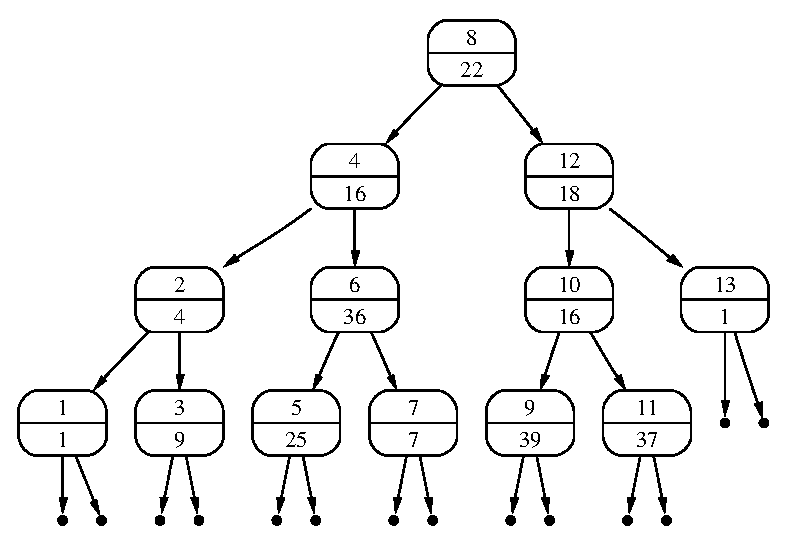
\epsfig{file=Abbildungen/graph1.eps}} 
  \caption{Ein geordneter bin�rer Baum}
  \label{fig:graph1}
\end{figure}


Wir �berlegen uns nun, wie wir mit Hilfe geordneter bin�rer B�ume den ADT \textsl{Map}
implementieren k�nnen.  Wir spezifizieren die einzelnen Methoden dieses Daten-Typs durch
bedingte Gleichungen.  Der Konstruktor $\textsl{map}()$ liefert als Ergebnis den leeren Baum zur�ck:
\[ \textsl{map}() = \textsl{Nil}. \]
F�r die Methode $\textsl{find}()$ erhalten wir die folgenden Gleichungen:
\begin{enumerate}
\item $\textsl{Nil}.\textsl{find}(k) = \Omega$,

      denn der leere Baum repr�sentiert die leere Abbildung.
\item $\textsl{Node}(k, v, l, r).\textsl{find}(k) = v$,

      denn der Knoten $\textsl{Node}(k,v,l,r)$ speichert die Zuordnung $k \mapsto v$.
\item $k_1 < k_2 \rightarrow \textsl{Node}(k_2, v, l, r).\textsl{find}(k_1) = l.\textsl{find}(k_1)$,

      denn wenn $k_1$ kleiner als $k_2$ ist, dann kann aufgrund der Ordnungs-Bedingung
      eine Zuordnung f�r $k_1$ nur in dem linken Teilbaum $l$ gespeichert sein.
\item $k_1 > k_2 \rightarrow \textsl{Node}(k_2, v, l, r).\textsl{find}(k_1) = r.\textsl{find}(k_1)$,

      denn wenn $k_1$ gr��er als $k_2$ ist, dann kann aufgrund der Ordnungs-Bedingung
      eine Zuordnung f�r $k_1$ nur in dem rechten Teilbaum $r$ gespeichert sein.
\end{enumerate}
Als n�chstes definieren wir die Funktion \textsl{insert}.  Die Definition erfolgt
ebenfalls mit Hilfe rekursiver Gleichungen und ist ganz analog zur Definition der 
Funktion \textsl{find}.
\begin{enumerate}
\item $\textsl{Nil}.\textsl{insert}(k,v) = \textsl{Node}(k,v, \textsl{Nil}, \textsl{Nil})$,
  
      denn wenn der Baum vorher leer ist, so kann die einzuf�gende Information direkt an
      der Wurzel abgespeichert werden.
\item $\textsl{Node}(k,v_2,l,r).\textsl{insert}(k,v_1) = \textsl{Node}(k, v_1, l, r)$,

      denn wenn wir den Schl�ssel $k$ an der Wurzel finden, �berschreiben wir einfach den zugeordneten 
      Wert.
\item $k_1 < k_2 \rightarrow 
         \textsl{Node}(k_2, v_2, l, r).\textsl{insert}(k_1, v_1) = \textsl{Node}(k_2, v_2, l.\textsl{insert}(k_1, v_1), r)$,

      denn wenn der Schl�ssel $k_1$, unter dem wir Informationen einf�gen wollen, kleiner
      als der Schl�ssel $k_2$ an der Wurzel ist, so m�ssen wir die einzuf�gende
      Information im linken Teilbaum einf�gen.
\item $k_1 > k_2 \rightarrow 
         \textsl{Node}(k_2, v_2, l, r).\textsl{insert}(k_1, v_1) = 
         \textsl{Node}(k_2, v_2, l, r.\textsl{insert}(k_1, v_1))$,

      denn wenn der Schl�ssel $k_1$, unter dem wir Informationen einf�gen wollen, gr��er
      als der Schl�ssel $k_2$ an der Wurzel ist, so m�ssen wir die einzuf�gende
      Information im rechten Teilbaum einf�gen.
\end{enumerate}
Als letztes definieren wir die Methode \textsl{delete}. Diese Definition ist schwieriger als
die Implementierung der andern beiden Methoden.  Falls wir in einen Baum der Form
$t =\textsl{Node}(k,v,l,r)$ den Eintrag mit dem Schl�ssel $k$ l�schen wollen, so
kommt es auf die beiden Teilb�ume $l$ und $r$ an.  Ist $l$ der leere Teilbaum,
so liefert $t.\textsl{delete}(k)$ als Ergebnis den Teilbaum $r$ zur�ck.
Ist $r$ der leere Teilbaum, so ist das Ergebnis $l$.  Problematisch ist die Situation,
wenn weder $l$ noch $r$ leer sind.  
Die L�sung besteht dann darin, dass wir in dem rechten
Teilbaum $r$ den Knoten mit dem kleinsten Schl�ssel suchen und diesen Knoten aus dem
Baum $r$ entfernen.  Den dadurch entstehenden Baum nennen wir $r'$.
 Anschlie�end �berschreiben wir in $t =\textsl{Node}(k,v,l,r')$ die
Werte $k$ und $v$ mit dem eben gefundenen kleinsten Schl�ssel $k_{min}$ und dem $k_{min}$
zugeordneten Wert $v_{min}$.  Der dadurch entstehende bin�re Baum 
$t=\textsl{Node}(k_{min},v_{min},l,r')$
 ist auch wieder
geordnet, denn einerseits ist der Schl�ssel $k_{min}$  gr��er als der Schl�ssel $k$ und
damit sicher auch gr��er als alle Schl�ssel im linken Teilbaum $l$ und andererseits ist
$k_{min}$ kleiner als alle  Schl�ssel im Teilbaum $r'$, denn $k_{min}$ ist ja der
kleinste Schl�ssel aus $r$.  

Zur Veranschaulichung betrachten wir ein Beispiel: Wenn wir in dem Baum aus Abbildung 
\ref{fig:graph1} den Knoten mit der Markierung $\pair(4,16)$ l�schen wollen,
so suchen wir zun�chst in dem Teilbaum, dessen Wurzel mit $\pair(6,36)$ markiert ist, den
Knoten, der mit dem kleinsten Schl�ssel markiert ist.  Dies ist der Knoten mit der
Markierung $\pair(5,25)$.  Wir l�schen diesen Knoten und �berschreiben die Markierung
$\pair(4,16)$ mit der Markierung $\pair(5,25)$.  Abbildung 
\ref{fig:graph2} auf Seite \pageref{fig:graph2} zeigt das Ergebnis.

\begin{figure}[!th]
  \centering
  \framebox{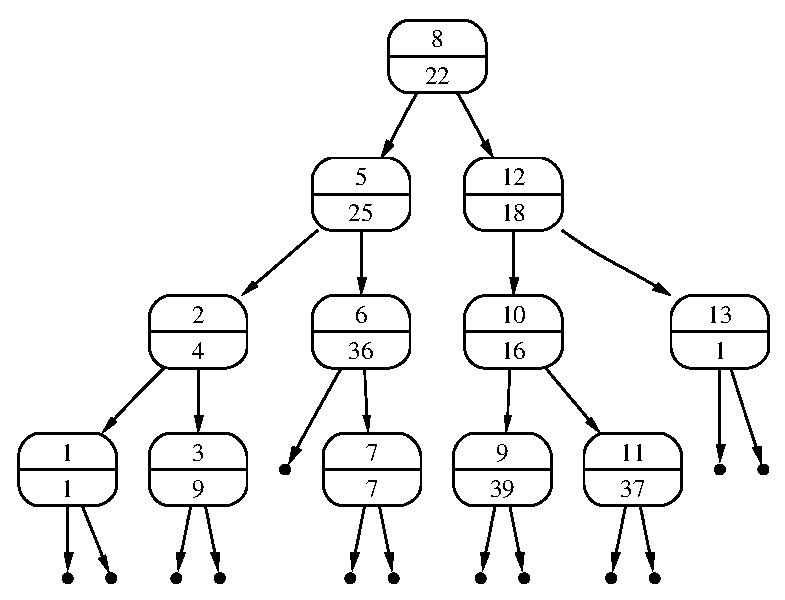
\epsfig{file=graph2.eps}} 
  \caption{Der geordnete bin�rer Baum aus Abbildung 
          \ref{fig:graph1} nach dem Entfernen des Knotens mit der Markierung $\pair(4,16)$.}
  \label{fig:graph2}
\end{figure}

Wir geben nun bedingte Gleichungen an, welche die Methode \textsl{delMin} spezifizieren.
\begin{enumerate}
\item $\textsl{Node}(k, v, \textsl{Nil}, r).\textsl{delMin}() = [r, k, v]$,

      denn wenn der linke Teilbaum leer ist, muss $k$ der kleinste Schl�ssel in 
      dem Baum sein.  Wenn wir diesen  Schl�ssel nebst dem zugeh�rigen Wert aus dem Baum
      entfernen, bleibt der rechte Teilbaum �brig.
\item $l\not= \textsl{Nil} \wedge l.\textsl{delMin}() = [l',k_{min}, v_{min}] \;\rightarrow$ \\[0.1cm]
       \hspace*{1.3cm} 
       $\textsl{Node}(k, v, l, r).\textsl{delMin}() = [\textsl{Node}(k, v, l', r), k_{min}, v_{min}]$,

      denn wenn der linke Teilbaum $l$ in dem bin�ren Baum $t = \textsl{Node}(k, v, l, r)$
      nicht leer ist, so muss der kleinste Schl�ssel von $t$ in $l$ liegen.
      Wir entfernen daher rekursiv den kleinsten Schl�ssel aus $l$ und erhalten dabei den
      Baum $l'$.  In dem urspr�nglich gegebenen Baum $t$ ersetzen wir $l$ durch $l'$ und erhalten
      $t = \textsl{Node}(k, v, l', r)$.
\end{enumerate}
Damit k�nnen wir nun die Methode $\mathtt{delete}()$ spezifizieren.
\begin{enumerate}
\item $\textsl{Nil}.\textsl{delete}(k) = \textsl{Nil}$.
\item $\textsl{Node}(k,v,\textsl{Nil},r).\textsl{delete}\bigl(k\bigr) = r$.
\item $\textsl{Node}(k,v,l,\textsl{Nil}).\textsl{delete}(k) = l$.
\item $l \not= \textsl{Nil} \,\wedge\, r \not= \textsl{Nil} \,\wedge\, r.\textsl{delMin}() = [r',k_{min}, v_{min}]  \;\rightarrow$ \\[0.1cm]
      \hspace*{1.3cm}
      $\textsl{Node}(k,v,l,r).\textsl{delete}(k) = \textsl{Node}(k_{min},v_{min},l,r')$.
      
      Falls der zu entfernende Schl�ssel mit dem Schl�ssel an der Wurzel des Baums
      �bereinstimmt,  entfernen wir mit dem Aufruf $r\mathtt{.}\textsl{delMin}()$
      den kleinsten Schl�ssel aus dem rechten Teilbaum  $r$ und produzieren dabei den Baum $r'$.
      Gleichzeitig berechnen wir dabei f�r den rechten Teilbaum den kleinsten Schl�ssel $k_{min}$ und den
      diesem Schl�ssel zugeordneten Wert $v_{min}$.  Diese Werte setzen wir nun an die
      Wurzel des neuen Baums.

\item $k_1 < k_2 \rightarrow \textsl{Node}(k_2,v_2,l,r).\textsl{delete}\bigl(k_1) = 
       \textsl{Node}(k_2,v_2,l.\textsl{delete}(k_1),r)$.

      Falls der zu entfernende Schl�ssel kleiner ist als der Schl�ssel an der Wurzel,
      so kann sich der Schl�ssel nur im linken Teilbaum befinden.  Daher wird der
      Schl�ssel $k_1$ rekursiv in dem linken Teilbaum $l$ entfernt.
\item $k_1 > k_2 \rightarrow \textsl{Node}(k_2,v_2,l,r).\textsl{delete}(k_1) = 
       \textsl{Node}(k_2,v_2,l,r.\textsl{delete}(k_1))$,

      denn in diesem Fall kann sich der Eintrag mit dem Schl�ssel $k_1$  nur in dem
      rechten Teilbaum $r$ befinden.
\end{enumerate}

\subsection{Implementing Ordered Binary Trees in \textsc{SetlX}}
Figure \ref{fig:binary-tree.stlx-1} and Figure \ref{fig:binary-tree.stlx-2} show how ordered binary
trees can be implemented in \textsc{SetlX}.  Objects of class \texttt{map} encapsulate ordered
binary trees.  We discuss the implementation of this class next.
\begin{enumerate}
\item The constructor map is called with one argument.  This argument, called \texttt{cmp}
      in line 1, is a function representing a total order ''$<$''.  The idea is that the function
      \texttt{cmp} is called with two arguments and we have
      \\[0.2cm]
      \hspace*{1.3cm}
      $\mathtt{cmp}(x,y)$ \quad if and only if \quad $x < y$.
      \\[0.2cm]
      The function \texttt{cmp} is later stored in the member variable \texttt{mCmpFct} in line 6.
\item The class \texttt{map} represents a node in an ordered binary tree.  In order to do so, it
      maintains four additional member variables.
      \begin{enumerate}
      \item \texttt{mKey} is the key stored at this node.  For an empty node, \texttt{mKey}
            has the value \texttt{om}, which represents $\Omega$.
      \item \texttt{mValue} stores the value stored at this node.  For an empty node,
            \texttt{mValue} is \texttt{om}.
      \item \texttt{mLeft} is the left subtree.  An empty subtree is represented as \texttt{om}.
      \item \texttt{mRight} is the right subtree.  
      \end{enumerate}
\item The function \texttt{isEmpty} checks whether \texttt{this} represents an empty tree.
      The assumption is that if \texttt{mKey} is \texttt{om}, then the member variables
      \texttt{mValue}, \texttt{mLeft}, and \texttt{mRight} will also be \texttt{om}.
\item The implementation of \texttt{find} works as follows:
      \begin{enumerate}
      \item If the node is empty, there is no value to find and the function returns \texttt{om}.
            Note that in \textsc{SetlX} a \texttt{return} statement which does not return a value 
            automatically returns \texttt{om}.
      \item If the key we are looking for is stored at the root of this tree, the value stored for
            this key is \texttt{mValue}.
      \item Otherwise, we have to compare the key \texttt{k}, which is the key we are looking for,
            with the key \texttt{mKey}, which is the key stored in this node.  If \texttt{k}
            is less than \texttt{mKey}, \texttt{k} can at most be stored in the left subtree
            \texttt{mLeft}, while if $k$ is greater than \texttt{mKey}, \texttt{k} can only be
            stored in the right subtree.
      \end{enumerate}


\begin{figure}[!ht]
  \centering
\begin{Verbatim}[ frame         = lines, 
                  framesep      = 0.3cm, 
                  labelposition = bottomline,
                  numbers       = left,
                  numbersep     = -0.2cm,
                  xleftmargin   = 0.0cm,
                  xrightmargin  = 0.0cm
                ]
    class map(cmp) {
        mKey    := om;
        mValue  := om; 
        mLeft   := om;
        mRight  := om;
        mCmpFct := cmp;  // function to compare keys
      static {
        isEmpty := [] |-> mKey == om;
        find := procedure(k) {
            if      (isEmpty())        { return;                }
            else if (mKey == k)        { return mValue;         }
            else if (mCmpFct(k, mKey)) { return mLeft .find(k); }
            else                       { return mRight.find(k); }
        };
        insert := procedure(k, v) {
              if (isEmpty()) { 
                this.mKey   := k;
                this.mValue := v; 
                this.mLeft  := map(mCmpFct);
                this.mRight := map(mCmpFct);
            } else if (mKey == k) { 
                mValue := v; 
            } else if (mCmpFct(k, mKey)) { 
                mLeft .insert(k, v); 
            } else { 
                mRight.insert(k, v); 
            }
        };
\end{Verbatim}
\vspace*{-0.3cm}
  \caption{Implementierung geordneter B�ume in \textsc{SetlX}, 1.~Teil.}
  \label{fig:binary-tree.stlx-1}
\end{figure}
\item The implementation of \texttt{insert} is similar to the implementation of \texttt{find}.
      \begin{enumerate}
      \item If the binary tree is empty, we set the member variables \texttt{mKey} and
            \texttt{mValue} to the appropriate values.  The member variables \texttt{mLeft} and 
            \texttt{mRight} are initialized as empty trees.
      \item If the key \texttt{k} under which the value \texttt{v} is to be inserted is identical
            to the key \texttt{mKey} stored at this node, then we have found the node where we need
            to insert \texttt{v}.  In this case, \texttt{mValue} is overwritten with \texttt{v}.
      \item Otherwise, \texttt{k} is compared with \texttt{mKey} and the search is continued in the
            appropriate subtree.
      \end{enumerate}      


\begin{figure}[!ht]
  \centering
\begin{Verbatim}[ frame         = lines, 
                  framesep      = 0.3cm, 
                  firstnumber   = last,
                  labelposition = bottomline,
                  numbers       = left,
                  numbersep     = -0.2cm,
                  xleftmargin   = 0.8cm,
                  xrightmargin  = 0.8cm
                ]
        delMin := procedure() {
            if (mLeft.isEmpty()) { 
                return [ mRight, mKey, mValue ]; 
            } else {
                 [ ls, km, vm ] := mLeft.delMin();
                 this.mLeft := ls;
                 return [ this, km, vm ];
            }
        };
        delete := procedure(k) {
            if      (isEmpty())  { return; } 
            else if (k == mKey)  {
                if      (mLeft .isEmpty()) { update(r); }  
                else if (mRight.isEmpty()) { update(l); } 
                else {
                    [ rs, km, vm ] := mRight.delMin();
                    this.mKey   := km;
                    this.mValue := vm; 
                    this.mRight := rs;
                }
            } else if (mCmpFct(k, mKey)) {
                if (!mLeft .isEmpty()) { mLeft.delete(k); }
            } else {
                if (!mRight.isEmpty()) { mRight.delete(k); }
            }
        };
        update := procedure(t) {
            this.mKey   := t.mKey;
            this.mValue := t.mValue;
            this.mLeft  := t.mLeft;
            this.mRight := t.mRight;
        };
      }
    }
\end{Verbatim}
\vspace*{-0.3cm}
  \caption{Ordered binary trees in \textsc{SetlX}, part2.}
  \label{fig:binary-tree.stlx-2}
\end{figure}

\item The implementation of \texttt{delMin} and \texttt{delete} is done in a similar way as the
      implementation of \texttt{insert}.  It should be noted that the implementation follows directly from the
      equations derived  previously. 
\end{enumerate}

\begin{figure}[!th]
  \centering 
  \framebox{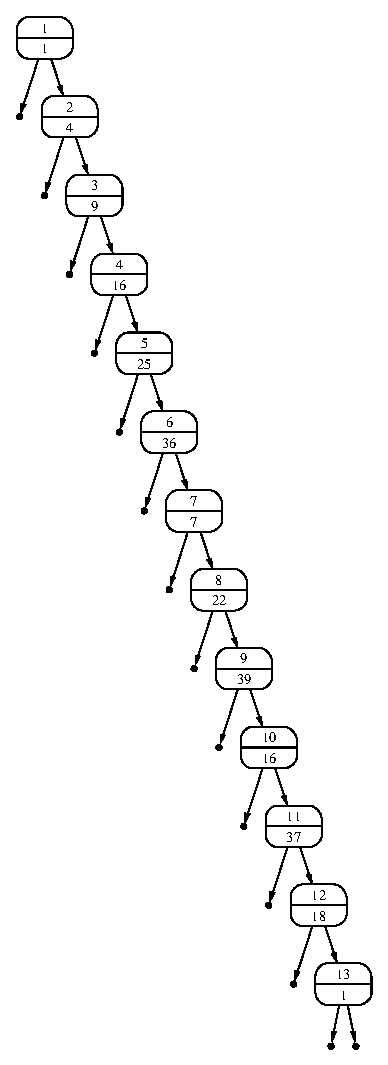
\epsfig{file=degenerated-bin-tree}} 
  \caption{Ein entarteter  geordneter bin�rer Baum.}
  \label{fig:degenerated}
\end{figure}


\subsection{Analysis of the Complexity}
In this section we will first discuss the worst case complexity, which is quite bad.  In fact, in
the worst case, the call $b.\mathtt{find}(k)$ will perform $\Oh(n)$ key comparisons if $b$ is an ordered
binary search tree of $n$ elements.  After that, we investigate the average case complexity.  We
will show that the average case complexity is $\Oh\bigr(\ln(n)\bigr)$.

\subsubsection{Worst Case Complexity}
We begin our investigation of the complexity with an analysis of the complexity of $b.\textsl{find}(k)$ 
in the worst case.  The worst case happens if the binary tree $b$ degenerates into a list.
Figure \ref{fig:degenerated} on page \pageref{fig:degenerated} shows the ordered binary tree that
is generated if the keys are inserted in increasing order.  If we then have to search for the
biggest key, we have to traverse the complete tree in order to find this key.  Therefore, if the
tree $b$ contains $n$ different keys, we have to compare the key $k$ that we are looking for to all
of these $n$ keys in the tree.  Hence, in this case the complexity of $b.\textsl{find}(k)$ is 
$\Oh(n)$ and this is the same complexity that we would have gotten if we had used a linked list.


\subsubsection{Average Case Complexity}
Fortunately, the worst case has a very small probability to occur. On average, a randomly generated
binary tree is quite well balanced.  We will show next that the number of comparisons necessary for
the function call $b.\textsl{find}(k)$ has the order $\Oh\bigl(\ln(n)\bigr)$.  


%Dazu definieren wir auf bin�ren B�umen zun�chst eine Funktion 
%\[ \textsl{height}: \Bin \rightarrow \N, \]
%die die H�he eines bin�ren Baums angibt.  Die Definition erfolgt induktiv.
%\begin{enumerate}
%\item $\textsl{Nil}.\textsl{height}() = 0$.

%      Der leere Baum hat die H�he $0$.
%\item $\textsl{node}(k,v,l,r).\textsl{height}() = 
%       1 + \max\bigl(l.\textsl{height}(),\, r.\textsl{height}()\bigr)$.

%      Die H�he des Baums $\textsl{node}(k,v,l,r)$ ist um eins gr��er als die H�he des
%      gr��ten Teilbaums.
%\end{enumerate}
%Analog definieren wir f�r einen bin�ren Baum $b$ die Anzahl $b.\textsl{count}()$ der Schl�ssel, die
%der Baum enth�lt.   Die Definition von $b.\textsl{count}()$ erfolgt durch Induktion nach $b$.
%\begin{enumerate}
%\item $\textsl{Nil}.\textsl{count}() = 0$.

%      Der leere Baum enth�lt keine Schl�ssel.
%\item $\textsl{node}(k,v,l,r).\textsl{count}() = 
%       1 + l.\textsl{count}() + r.\textsl{height}()\bigr)$.

%      Der Baum $\textsl{node}(k,v,l,r)$ enth�lt zus�tzlich zu dem Schl�ssel $k$ die
%      Schl�ssel aus den Teilb�umen $l$ und $r$.
%\end{enumerate}
%Der folgende Satz zeigt, wieviel Schl�ssel ein Baum der H�he $h$ h�chstens enthalten
%kann.

%\begin{Satz}
%  Ein bin�rer Baum $b$ der H�he $h$ enth�lt h�chstens $2^h - 1$ Schl�ssel.
%\end{Satz}
%\noindent
%\textbf{Beweis}:  Wir bezeichnen die maximale Anzahl Schl�ssel eines Baums der H�he $h$
%mit $c_h$.  Wir beweisen  durch Induktion nach $h$, dass gilt:
%\[ c_h = 2^h - 1. \]
%\begin{enumerate}
%\item[I.A.] $h = 0$: Der einzige Baum der H�he $0$ ist $\textsl{Nil}$.
%            Dieser enth�lt $0$ Schl�ssel.  Also gilt
%            \\[0.2cm]
%            \hspace*{1.3cm}
%            $c_0 = 0 = 2^0 - 1$.
%\item[I.S.] $h \mapsto h + 1$: Ein Baum der H�he $h+1$, der die maximale Anzahl
%            Schl�ssel enth�lt, hat die Form $\textsl{node}(k,v,l,r)$, wobei dann $l$ und
%            $r$  B�ume der H�he $h$ sind, die die maximale Anzahl Schl�ssel enthalten.
%            Folglich gilt:
%            \begin{eqnarray*}
%               c_{h+1} &               =  & 1 + c_h + c_h \\
%                       & \stackrel{IV}{=} & 1 + (2^h - 1) + (2^h - 1) \\
%                       &               =  & 2 \cdot 2^h - 1 \\
%                       &               =  & 2^{h+1} - 1. \hspace*{9cm} \Box
%            \end{eqnarray*}
%\end{enumerate}

%Die H�he eines Baumes gibt ein Ma� f�r die Komplexit�t der Methoden \textsl{find},
%\textsl{insert} und \textsl{delete}, denn bei einem Baum der H�he $h$ sind f�r jede dieser
%Operationen h�chstens $h$ Vergleiche von Schl�sseln erforderlich.

In order to prove this claim, we have to introduce some definitions.
We define the \underline{avera}g\underline{e} number of comparisons that are needed for the function
call $b.\textsl{find}(k)$ as  $d_n$, where $n$ is the number of keys stored in $b$.  We assume that
the key $k$ is indeed stored in $b$.  Our first goal is to derive a recurrence equation for 
$d_n$.  First, we note that  
\\[0.2cm]
\hspace*{1.3cm} $d_1 = 1$,
\\[0.2cm]
because if the tree $b$ contains only one key we will do exactly one key comparison,
Next, imagine a binary tree $b$ that contains $n+1$ keys.  Then $b$
can be written as 
\\[0.2cm]
\hspace*{1.3cm}
$b = \textsl{node}(k',v,l,r)$,
\\[0.2cm]
where $k'$ is the key at the root of $b$.  If the keys of $b$ are ordered as a list, then this
ordering looks something like the following:
\\[0.2cm]
\hspace*{1.3cm}
$k_0 < k_1 < \cdots < k_{i-1} < k_{i} < k_{i+1} < \cdots < k_{n-1} < k_n$.
\\[0.2cm]
Here are $n+1$ positions for the key $k'$.
If we have $k' = k_i$, then the left subtree of $b$ contains  $i$ keys while the right subtree
contains the remaining  $n-i$ keys:
\\[0.2cm]
\hspace*{1.3cm}
$\underbrace{k_0 < k_1 < \cdots < k_{i-1}}_{\mbox{keys in $l$}} < 
 \underbrace{k_{i}}_{\stackrel{\displaystyle \shortparallel}{\displaystyle k'}} < 
 \underbrace{k_{i+1} < \cdots < k_{n-1} < k_n}_{\mbox{keys in $r$}}$,
\\[0.2cm]
As  $b$ contains $n+1$ keys all together, there are  $n+1$ different possibilities for the position
of $k'$, as the number of keys in the left subtree $l$ is $i$ where
\\[0.2cm]
\hspace*{1.3cm}
 $i \in \{0,1, \cdots, n\}$.
\\[0.2cm]
Of course, if the left subtree has $i$ keys, the right subtree will have $n-i$ keys.
Let us denote the average number of comparisons that are done during the function call
$b.\textsl{find}(k)$ provided the left subtree of $b$ has $i$ keys while $b$ itself has $n+1$ keys
as
\\[0.2cm]
\hspace*{1.3cm}
$\textsl{numCmp}(i,\, n\!+\!1)$.
\\[0.2cm]
Then, since all values of $i$ have the same probability, we have
\\[0.2cm]
\hspace*{1.3cm}
$\ds d_{n+1} =  \frac{1}{n+1} \cdot \sum\limits_{i=0}^n \textsl{numCmp}(i,\, n\!+\!1)$.
\\[0.2cm]
We proceed to compute $\textsl{numCmp}(i,n\!+\!1)$:
If  $l$ contains $i$ keys while $r$ contains the remaining $n-i$ keys,
then there are three possibilities for the key $k$ that we want to find in $b$:
\begin{enumerate}
\item $k$ might be identical with the key $k'$ that is located at the root of $b$.
      In this case there is only one comparison.
      Now there  are $n+1$ keys in $b$ and the key we are looking for will be at the root in only
      one of these cases, the probability of this case is
      \\[0.2cm]
      \hspace*{1.3cm} $\bruch{1}{\,n+1\,}$.

\item $k$ might be identical to one of the  $i$ keys of the left subtree $l$.
      The probability for this case is 
      \\[0.2cm]
      \hspace*{1.3cm} $\displaystyle\bruch{i}{n+1}$. \\[0.2cm]
      In this case we need 
      \\[0.2cm]
      \hspace*{1.3cm} $\displaystyle d_i + 1$ \\[0.2cm]
      comparisons because in addition to the  $d_i$ comparisons in the left subtree we have to
      compare the key $k$ we are looking for with the key $k'$ at the root of the tree.
\item $k$ might be a key in the right subtree $r$.  As there are  $n-i$ keys in the right subtree
      and the total of keys is $n+1$, the probability that the key  $k$ occurs in the right subtree $r$
      is \\[0.2cm]
      \hspace*{1.3cm} $\displaystyle \bruch{n-i}{n+1}$. \\[0.2cm]
      Hence, in this case there are  \\[0.2cm]
      \hspace*{1.3cm} $\displaystyle d_{n-i} + 1$ \\[0.2cm]
      comparisons. 
\end{enumerate}
In order to compute  $\textsl{numCmp}(i, n\!+\!1)$ we have to multiply the probabilities in every
case with the number of comparisons and these three numbers have to added.  This yields
\begin{eqnarray*}
  \textsl{numCmp}(i, n\!+\!1) 
& = & \bruch{1}{\,n+1\,} \cdot 1 + \bruch{i}{n+1} \cdot (d_i + 1) + \bruch{n-i}{n+1} \cdot (d_{n-i} + 1) 
      \\[0.2cm]
& = & \bruch{1}{\,n+1\,} \cdot \bigl(1 + i \cdot (d_i + 1) + (n-i) \cdot (d_{n-i} + 1)\bigr)      \\[0.2cm]
& = & \bruch{1}{\,n+1\,} \cdot \bigl(1 + i + (n-i) + i \cdot d_i + (n-i) \cdot d_{n-i} \bigr)    \\[0.2cm]
& = & \bruch{1}{\,n+1\,} \cdot \bigl(n + 1 + i \cdot d_i + (n-i) \cdot d_{n-i} \bigr)            \\[0.2cm]
& = & 1 + \bruch{1}{\,n+1\,} \cdot \bigl(i \cdot d_i + (n-i) \cdot d_{n-i} \bigr) 
\end{eqnarray*}


Therefore, the recurrence equation for $d_{n+1}$ is given as follows: 
\\[0.2cm]
\hspace*{1.3cm}
$
\begin{array}{lcl}
d_{n+1} 
& = &  
\ds\sum\limits_{i=0}^n \bruch{1}{\,n+1\,} \cdot \textsl{numCmp}(i,\,n\!+\!1)  \\[0.5cm]
& = &  
\ds\bruch{1}{n+1} \cdot \sum\limits_{i=0}^n  
           \left(1 + \bruch{1}{n+1} \cdot \bigl(i \cdot d_i + (n-i) \cdot d_{n-i} \bigr) \right)
\\[0.5cm]
& = &  
\bruch{1}{n+1} \cdot \Biggl(\underbrace{\sum\limits_{i=0}^n 1}_{\stackrel{\displaystyle \shortparallel}{n+1}} \;+\;
           \bruch{1}{n+1} \cdot \ds\sum\limits_{i=0}^n \bigl(i \cdot d_i + (n-i) \cdot d_{n-i} \bigr) \Biggr)
\\[1.3cm]
& = &  
1 + \bruch{1}{(n+1)^2} \cdot \left(\ds\sum\limits_{i=0}^n \left(i\cdot d_i + (n-i)\cdot d_{n-i}\right) \right) 
\\[0.5cm]
& = &  
1 + \bruch{2}{(n+1)^2} \cdot \ds\sum\limits_{i=0}^n i\cdot d_i 
\end{array}
$
\\[0.2cm]
Here we have used the equation  \\[0.2cm]
\hspace*{1.3cm}
$\ds\sum\limits_{i=0}^n f(n-i) = \sum\limits_{i=0}^n f(i)$. \\[0.2cm]
We had verified this equation already when discussing the complexity of Quick Sort in the average
case.  Next, we solve the recurrence equation 
\begin{equation}
  \label{eq:bin1}
d_{n+1} = \displaystyle 1 + \bruch{2}{(n+1)^2} \cdot \sum\limits_{i=0}^n i\cdot d_i  
\end{equation}
with the initial condition $d_1 = 1$.  
In order to solve the equation (\ref{eq:bin1}) we perform the substitution $n \mapsto n+1$.  This yields
\begin{equation}
  \label{eq:bin2}
d_{n+2} = \displaystyle 1 + \bruch{2}{(n+2)^2} \cdot \sum\limits_{i=0}^{n+1} i\cdot d_i  
\end{equation}
We multiply equation (\ref{eq:bin1}) with $(n+1)^2$ and equation (\ref{eq:bin2}) 
with $(n+2)^2$.  We get
\begin{eqnarray}
  \label{eq:bin3}
(n+1)^2 \cdot d_{n+1} & = & (n+1)^2 + 2 \cdot \sum\limits_{i=0}^n i\cdot d_i, \\
  \label{eq:bin4}
(n+2)^2 \cdot d_{n+2} & = & (n+2)^2 + 2 \cdot \sum\limits_{i=0}^{n+1} i\cdot d_i
\end{eqnarray}
We subtract equation  (\ref{eq:bin3}) from equation (\ref{eq:bin4})
and are left with \\[0.2cm]
\hspace*{1.3cm} 
$(n+2)^2 \cdot d_{n+2} - (n+1)^2 \cdot d_{n+1} = (n+2)^2 - (n+1)^2 + 2 \cdot (n+1) \cdot d_{n+1}$.
\\[0.2cm]
To simplify this equation we substitute  $n \mapsto n - 1$ and get \\[0.2cm]
\hspace*{1.3cm} 
$(n+1)^2 \cdot d_{n+1} - n^2 \cdot d_{n} = (n+1)^2 - n^2 + 2 \cdot n \cdot d_{n}$.
\\[0.2cm]
This can be simplified as \\[0.2cm]
\hspace*{1.3cm} $(n+1)^2 \cdot d_{n+1}  =  n \cdot (n + 2) \cdot d_{n} + 2 \cdot n + 1$. \\[0.2cm]
Let us divide both sides of this equation by $(n+2)\cdot (n+1)$.  We get \\[0.2cm]
\hspace*{1.3cm}  
$\displaystyle \bruch{n+1}{n+2} \cdot d_{n+1}  =  \bruch{n}{n + 1} \cdot d_{n} + \bruch{2 \cdot n + 1}{(n+2)\cdot (n+1)}$. \\[0.2cm]
We define \\[0.2cm]
\hspace*{1.3cm} $\displaystyle c_n = \bruch{n}{n+1} \cdot d_n$. \\[0.4cm]
Then $c_1 = \bruch{1}{2} \cdot d_1 = \bruch{1}{2}$ and hence we have found the recurrence equation \\[0.2cm]
\hspace*{1.3cm} 
$\displaystyle c_{n+1}  =  c_{n} + \frac{2 \cdot n + 1}{(n+2)\cdot (n+1)}$. \\[0.2cm]
A partial fraction decomposition shows \\[0.2cm]
\hspace*{1.3cm} 
$\displaystyle \frac{2 \cdot n + 1}{(n+2)\cdot (n+1)} = \frac{3}{n+2} - \frac{1}{n+1}$. \\[0.2cm]
Hence we have \\[0.2cm]
\hspace*{1.3cm} $\displaystyle c_{n+1} = c_n +  \frac{3}{n+2} - \frac{1}{n+1}$. \\[0.2cm]
Because of $c_1 = \bruch{1}{2}$ this equation is also valid for  $n=0$ if we define $c_0 = 0$, since
we have
\\[0.2cm]
\hspace*{1.3cm}
$\bruch{1}{2} = 0 + \bruch{3}{0+2} - \bruch{1}{0+1}$.
\\[0.2cm]
The recurrence equation for $c_n$ can be solved using  telescoping:
\begin{eqnarray*}  
  c_{n+1} & = & c_0 + \sum\limits_{i=0}^{n} \frac{3}{i+2} - \sum\limits_{i=0}^{n} \frac{1}{i+1} 
\\[0.2cm]
          & = & \sum\limits_{i=2}^{n+2} \frac{3}{i} - \sum\limits_{i=1}^{n+1} \frac{1}{i}.
\end{eqnarray*}
To simplify this equation we substitute $n \mapsto n-1$ and get
\\[0.2cm]
\hspace*{1.3cm}
$c_{n} =  \displaystyle\sum\limits_{i=2}^{n+1} \frac{3}{i} - \sum\limits_{i=1}^{n} \frac{1}{i}$
\\[0.2cm]
The harmonic number  $H_n$ is defined as 
$H_n = \ds\sum\limits_{i=1}^{n} \bruch{1}{i}$.   
Therefore,  $c_n$ can be reduced to $H_n$: 
\\[0.2cm]
\hspace*{1.3cm}
$c_n = \ds 3 \cdot H_n - \frac{3}{1} + \frac{3}{n+1} - H_n  =  \ds 2 \cdot H_n - 3 \cdot \frac{n}{n+1}$
\\[0.2cm] 
Because $H_n = \displaystyle\sum\limits_{i=1}^{n} \frac{1}{i} = \ln(n) + \Oh(1)$ and $\ds 3 \cdot\frac{n}{n+1} \in \Oh(1)$
we therefore have
  \\[0.3cm]
\hspace*{1.3cm} 
$\displaystyle c_n = 2 \cdot \ln(n) + \Oh(1)$.
\\[0.3cm]
Because of  $d_n = \bruch{n+1}{n}\cdot c_n$ we have \\[0.2cm]
\hspace*{1.3cm}
 $\displaystyle d_n = 2 \cdot \ln(n) + \Oh\bigl(1\bigr)$.
\\[0.2cm]
This is our main result:  On average, the operation $b.\textsl{find}(k)$ uses
\\[0.2cm]
\hspace*{1.3cm}
$2 \cdot \ln(n) = 2 \cdot \ln(2) \cdot \log_2(n) \approx 1.386 \cdot \log_2(n)$ 
\\[0.2cm]
comparisons.  Hence there are about  39 \% 
more comparisons than if we had a tree which was  optimal balanced.
There are similar results for the operations \textsl{insert} and \textsl{delete}.


%%% Local Variables: 
%%% mode: latex
%%% TeX-master: "algorithms"
%%% End: 


\section{AVL-B�ume}
Es gibt verschiedene Varianten von geordneten bin�ren B�umen, bei denen auch im
schlechtesten Fall die Anzahl der Vergleiche nur logarithmisch von der Zahl der Schl�ssel
abh�ngt.  Eine solche Variante sind die \emph{AVL-B�ume} \cite{adelson:62}, die nach ihren Erfindern
G.~M.~Adel'son-Vel'ski\u{\i} und E.~M.~Landis benannt sind.  Diese Variante stellen wir jetzt vor.
Dazu definieren wir zun�chst die \emph{H�he} eines bin�ren Baums:
\begin{enumerate}
\item $\textsl{Nil}.\textsl{height}() = 0$.
\item $\textsl{Node}(k,v,l,r).\textsl{height}() = 
       \max\bigl( l.\textsl{height}(), r.\textsl{height}() \bigr) + 1$.
\end{enumerate}

\begin{Definition}[AVL-Baum] \hspace*{\fill} \\
{\em 
  Wir definieren die Menge $\AVL$ der \emph{AVL-B�ume} induktiv:
  \begin{enumerate}
  \item $\textsl{Nil} \in \AVL$.
  \item $\textsl{Node}(k,v,l,r) \in \AVL$ \quad g.d.w. 
        \begin{enumerate}
        \item $\textsl{Node}(k,v,l,r) \in \Bin_<$,
        \item $l, r \in \AVL$ \quad und
        \item $|l.\textsl{height}() - r.\textsl{height}()| \leq 1$.

              Diese Bedingungen bezeichnen wir auch als die \emph{Balancierungs-Bedingung}.
        \end{enumerate}
        AVL-B�ume sind also geordnete bin�re B�ume, f�r die sich an jedem Knoten
        $\textsl{Node}(k,v,l,r)$ die H�hen der Teilb�ume $l$ und $r$ maximal um 1
        unterscheiden.  \hspace*{\fill} $\Box$
  \end{enumerate}
}  
\end{Definition}


Um  AVL-B�ume zu  implementieren, k�nnen wir auf unserer Implementierung der geordneten
bin�ren B�ume aufsetzen. 
Neben den Methoden, die wir schon aus der Klasse \textsl{Map} kennen, brauchen wir noch
die Methode \\[0.2cm]
\hspace*{1.3cm} $\textsl{restore}: \Bin_< \rightarrow \AVL$, \\[0.2cm]
mit der wir die Balancierungs-Bedingung wiederherstellen k�nnen, wenn diese beim Einf�gen oder
L�schen eines Elements verletzt wird.  
Der Aufruf $b.\textsl{restore}()$ setzt voraus, dass $b$ ein geordneter bin�rer Baum ist,
f�r den au�er an der Wurzel �berall die Balancierungs-Bedingung erf�llt ist.
An der Wurzel kann die H�he des linken Teilbaums um maximal 2 von der H�he des rechten
Teilbaums abweichen. Beim Aufruf der Methode $b.\textsl{restore}()$ liegt also einer der
beiden folgenden F�lle vor: 
\begin{enumerate}
\item $b = \textsl{Nil}$ \quad oder
\item $b = \textsl{Node}(k,v,l,r) \wedge l \in \AVL \wedge r \in \AVL \wedge
       |l.\textsl{height}() - r.\textsl{height}()| \leq 2$.
\end{enumerate}
 Wir spezifizieren die Methode $\textsl{restore}$ durch
bedingte Gleichungen.
\begin{enumerate}
\item $\textsl{Nil}.\textsl{restore}() = \textsl{Nil}$,

      denn der leere Baum ist ein AVL-Baum.
\item $|l.\textsl{height}() - r.\textsl{height}()| \leq 1 \rightarrow 
       \textsl{Node}(k,v,l,r).\textsl{restore}() = \textsl{Node}(k,v,l,r)$,

      denn wenn die Balancierungs-Bedingung bereits erf�llt ist,
      braucht nichts getan werden.
\item $\begin{array}[t]{cl}
              & l_1.\textsl{height}() = r_1.\textsl{height}() + 2    \\ 
       \wedge & l_1 = \textsl{Node}(k_2,v_2,l_2,r_2)                 \\
       \wedge & l_2.\textsl{height}() \geq r_2.\textsl{height}()     \\[0.2cm]
       \rightarrow & \textsl{Node}(k_1,v_1,l_1,r_1).\textsl{restore}() = 
                     \textsl{Node}\bigl(k_2,v_2,l_2,\textsl{Node}(k_1,v_1,r_2,r_1)\bigr)
       \end{array}
      $

      Um diese Gleichung zu verstehen, betrachten wir Abbildung \ref{fig:casell}
      auf Seite \pageref{fig:casell}.  Der linke Teil der Abbildung beschreibt die
      Situation vor dem Ausbalancieren, es wird also der Baum \\[0.2cm]
      \hspace*{1.3cm} $\textsl{Node}(k_1,v_1, \textsl{Node}(k_2,v_2,l_2,r_2), r_1)$ \\[0.2cm]
      dargestellt.  Der rechte Teil der Abbildung zeigt das Ergebnis des
      Ausba\-lancierens, es wird also der Baum \\[0.2cm]
      \hspace*{1.3cm} $\textsl{Node}\bigl(k_2,v_2,l_2,\textsl{Node}(k_1,v_1,r_2,r_1)\bigr)$ \\[0.2cm]
      dargestellt. Wir haben hier die H�hen der einzelnen Teilb�ume jeweils in die
      zweiten Zeilen der entsprechenden Markierungen geschrieben.  Hier ist $h$ die H�he
      des Teilbaums $l_2$. Der Teilbaum $r_1$ hat die H�he $h - 1$.  Der Teilbaum $r_2$
      hat die H�he $h'$ und es gilt $h' \leq h$. Da $r_2$ ein AVL-Baum ist, gilt also
      entweder $h' = h$ oder $h' = h-1$.

      Die gezeigte Situation kann entstehen,
      wenn im linken Teilbaum $l_2$ ein Element eingef�gt wird oder wenn im rechten
      Teilbaum $r_1$ eine Element gel�scht wird.

      \begin{figure}[!ht]
        \centering
        \framebox{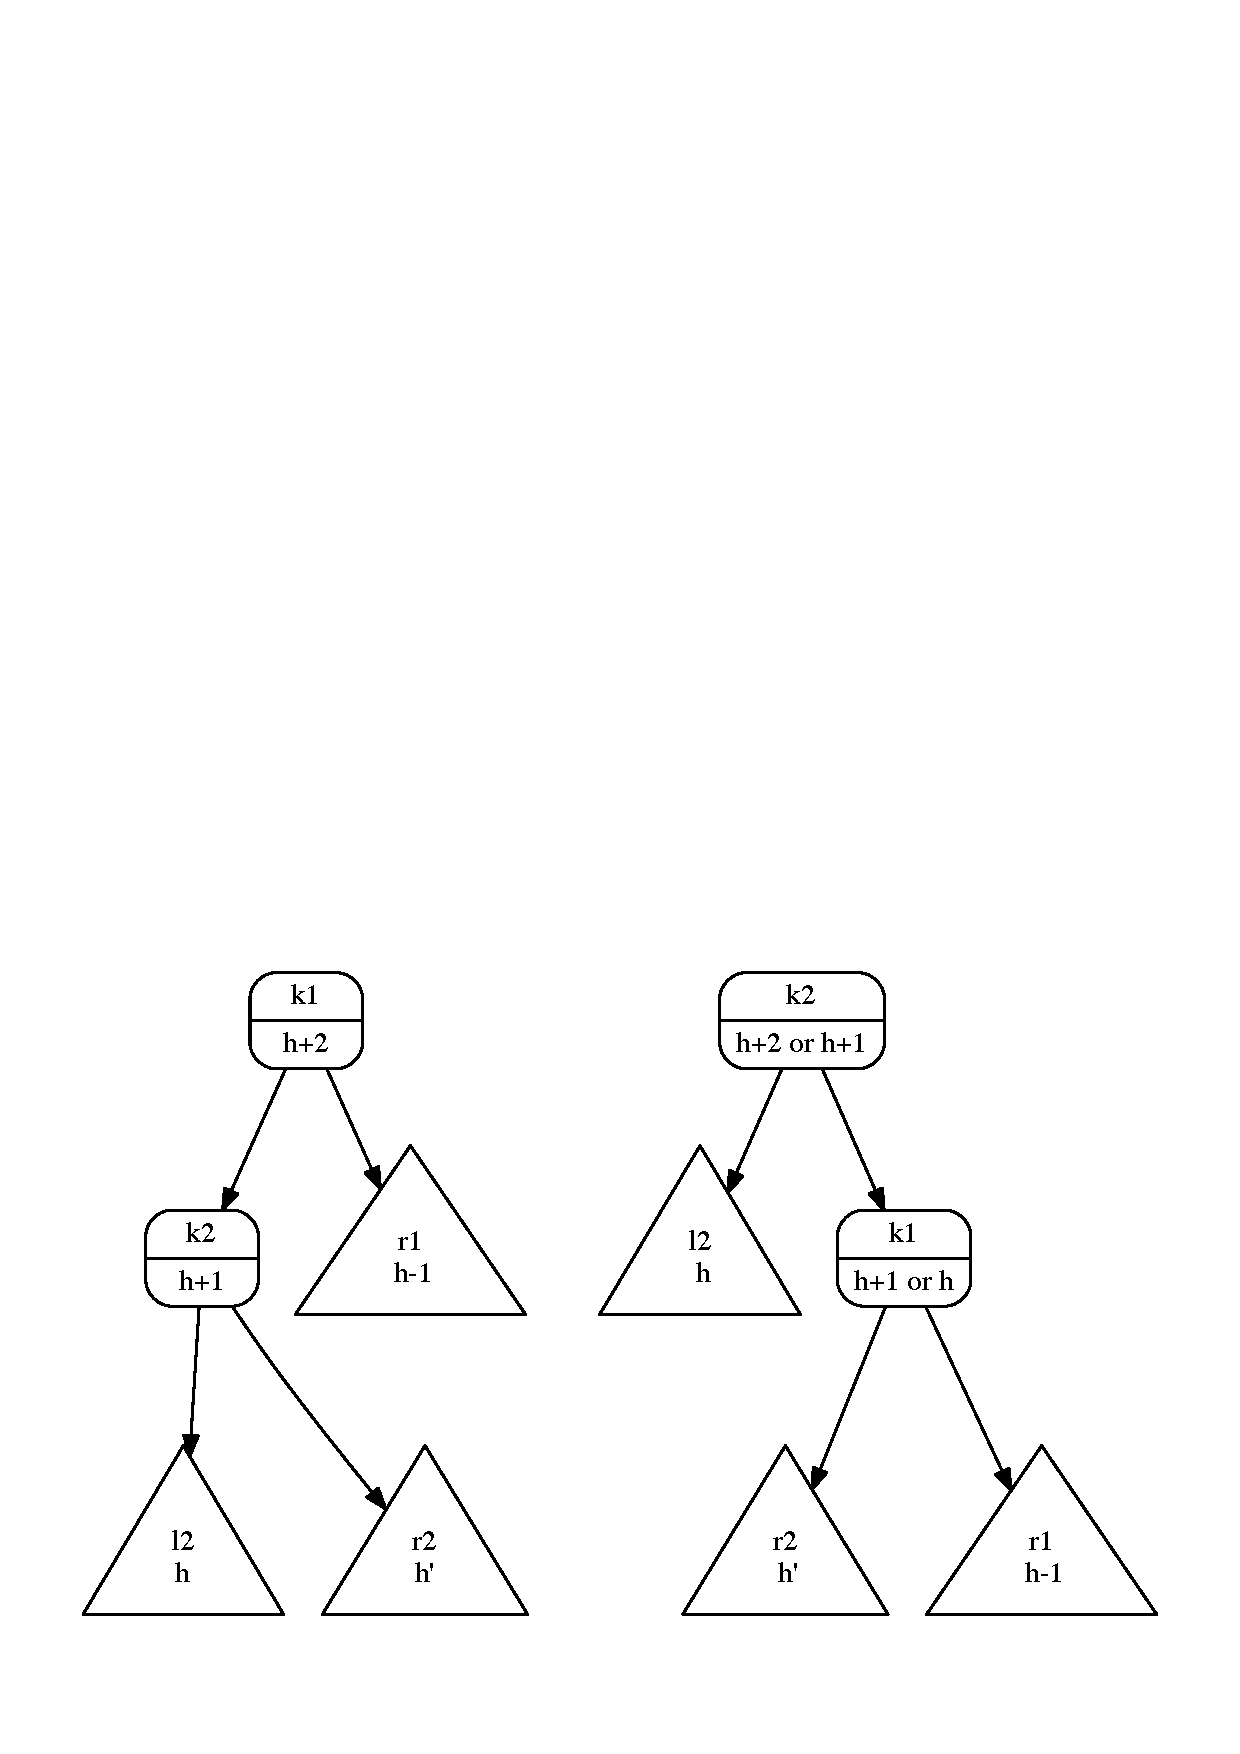
\epsfig{file=casell,scale=0.7}} 
        \caption{Ein unbalancierter Baum und der rebalancierte Baum}
        \label{fig:casell}
      \end{figure}

      Wir m�ssen uns davon �berzeugen, dass der im rechten Teil von Abbildung
      \ref{fig:casell} gezeigte Baum auch tats�chlich ein AVL-Baum ist.   Was die
      Balancierungs-Bedingung angeht, so rechnet man dies sofort nach.  Die Tatsache,
      dass der mit $k_1$ markierte Knoten entweder die H�he $h$ oder $h+1$ hat folgt
      daraus, dass $r_1$ die H�he $h-1$ hat und dass $h' \in \{h, h-1\}$ gilt.

      Um zu sehen, dass
      der Baum geordnet ist, k�nnen wir  folgende Ungleichung hinschreiben: \\[0.2cm]
      \hspace*{1.3cm} $l_2 < k_2 < r_2 < k_1 < r_1$. \hspace*{\fill} $(\star)$\\[0.2cm]
      Dabei  schreiben wir f�r einen Schl�ssel $k$ und einen bin�ren Baum $b$ \\[0.2cm]
      \hspace*{1.3cm} $k < b$ \\[0.2cm]
      um auzudr�cken, dass $k$ kleiner ist als alle Schl�ssel, die in dem Baum $b$ vorkommen.
      Analog schreiben wir $b < k$ wenn alle Schl�ssel, die in dem Baum $b$ vorkommen,
      kleiner sind als der Schl�ssel $k$.  Die Ungleichung $(\star)$ beschreibt die Anordnung
      der Schl�ssel sowohl f�r den im linken Teil der Abbildung gezeigten Baum als auch
      f�r den Baum im rechten Teil der Abbildung und damit sind beide B�ume geordnet.
\item $\begin{array}[t]{cl}
               & l_1.\textsl{height}() = r_1.\textsl{height}() + 2    \\ 
        \wedge & l_1 = \textsl{Node}(k_2,v_2,l_2,r_2)               \\
        \wedge & l_2.\textsl{height}() < r_2.\textsl{height}()     \\
        \wedge & r_2 = \textsl{Node}(k_3,v_3,l_3,r_3)               \\
        \rightarrow & \textsl{Node}(k_1,v_1,l_1,r_1).\textsl{restore}() = 
                      \textsl{Node}\bigl(k_3,v_3,\textsl{Node}(k_2,v_2,l_2,l_3),\textsl{Node}(k_1,v_1,r_3,r_1) \bigr)
        \end{array}
       $

        Die linke Seite der  Gleichung wird durch die Abbildung \ref{fig:caselr} auf Seite
        \pageref{fig:caselr}
        illustriert.  Dieser Baum kann in der Form \\[0.2cm]
        \hspace*{1.3cm} 
        $\textsl{Node}\bigl(k_1,v_1,\textsl{Node}(k_2,v_2,l_2,\textsl{Node}\bigl(k_3,v_3,l_3,r_3)\bigr),r_1\bigr)$ \\[0.2cm]
        geschrieben werden. Die Teilb�ume $l_3$ und $r_3$ haben hier entweder die H�he $h$ oder
        $h-1$, wobei mindestens einer der beiden Teilb�ume die H�he $h$ haben muss.
\begin{figure}[!ht]
  \centering
  \framebox{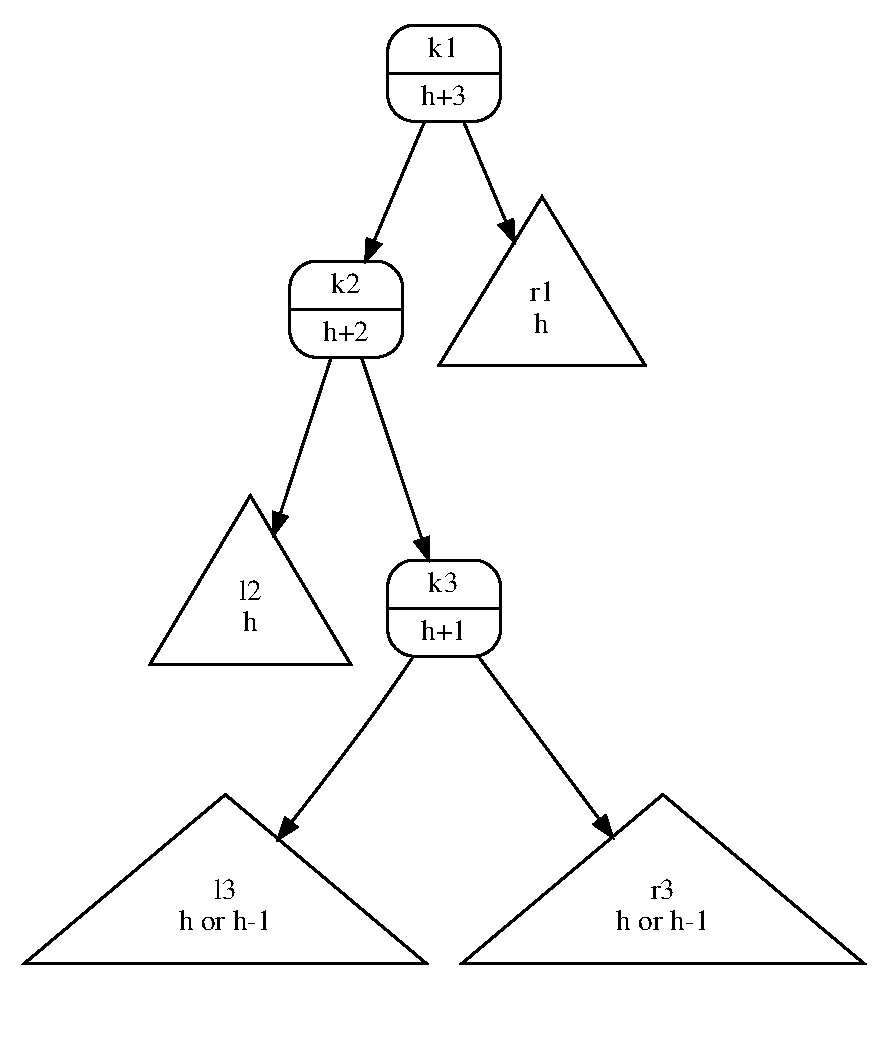
\epsfig{file=caselr,scale=0.7}} 
  \caption{Ein unbalancierter Baum: 2. Fall}
  \label{fig:caselr}
\end{figure}

     Die Situation der rechten Seite der obigen Gleichung zeigt Abbildung
     \ref{fig:caselr-nach} auf Seite \pageref{fig:caselr-nach}.  Der auf dieser
     Abbildung gezeigte Baum hat die Form \\[0.2cm]
     \hspace*{1.3cm} 
     $\textsl{Node}\bigl(k_3,v_3,\textsl{Node}(k_2,v_2,l_2,l_3),\textsl{Node}(k_1,v_1,r_3,r_1) \bigr)$.


\begin{figure}[!ht]
  \centering
  \framebox{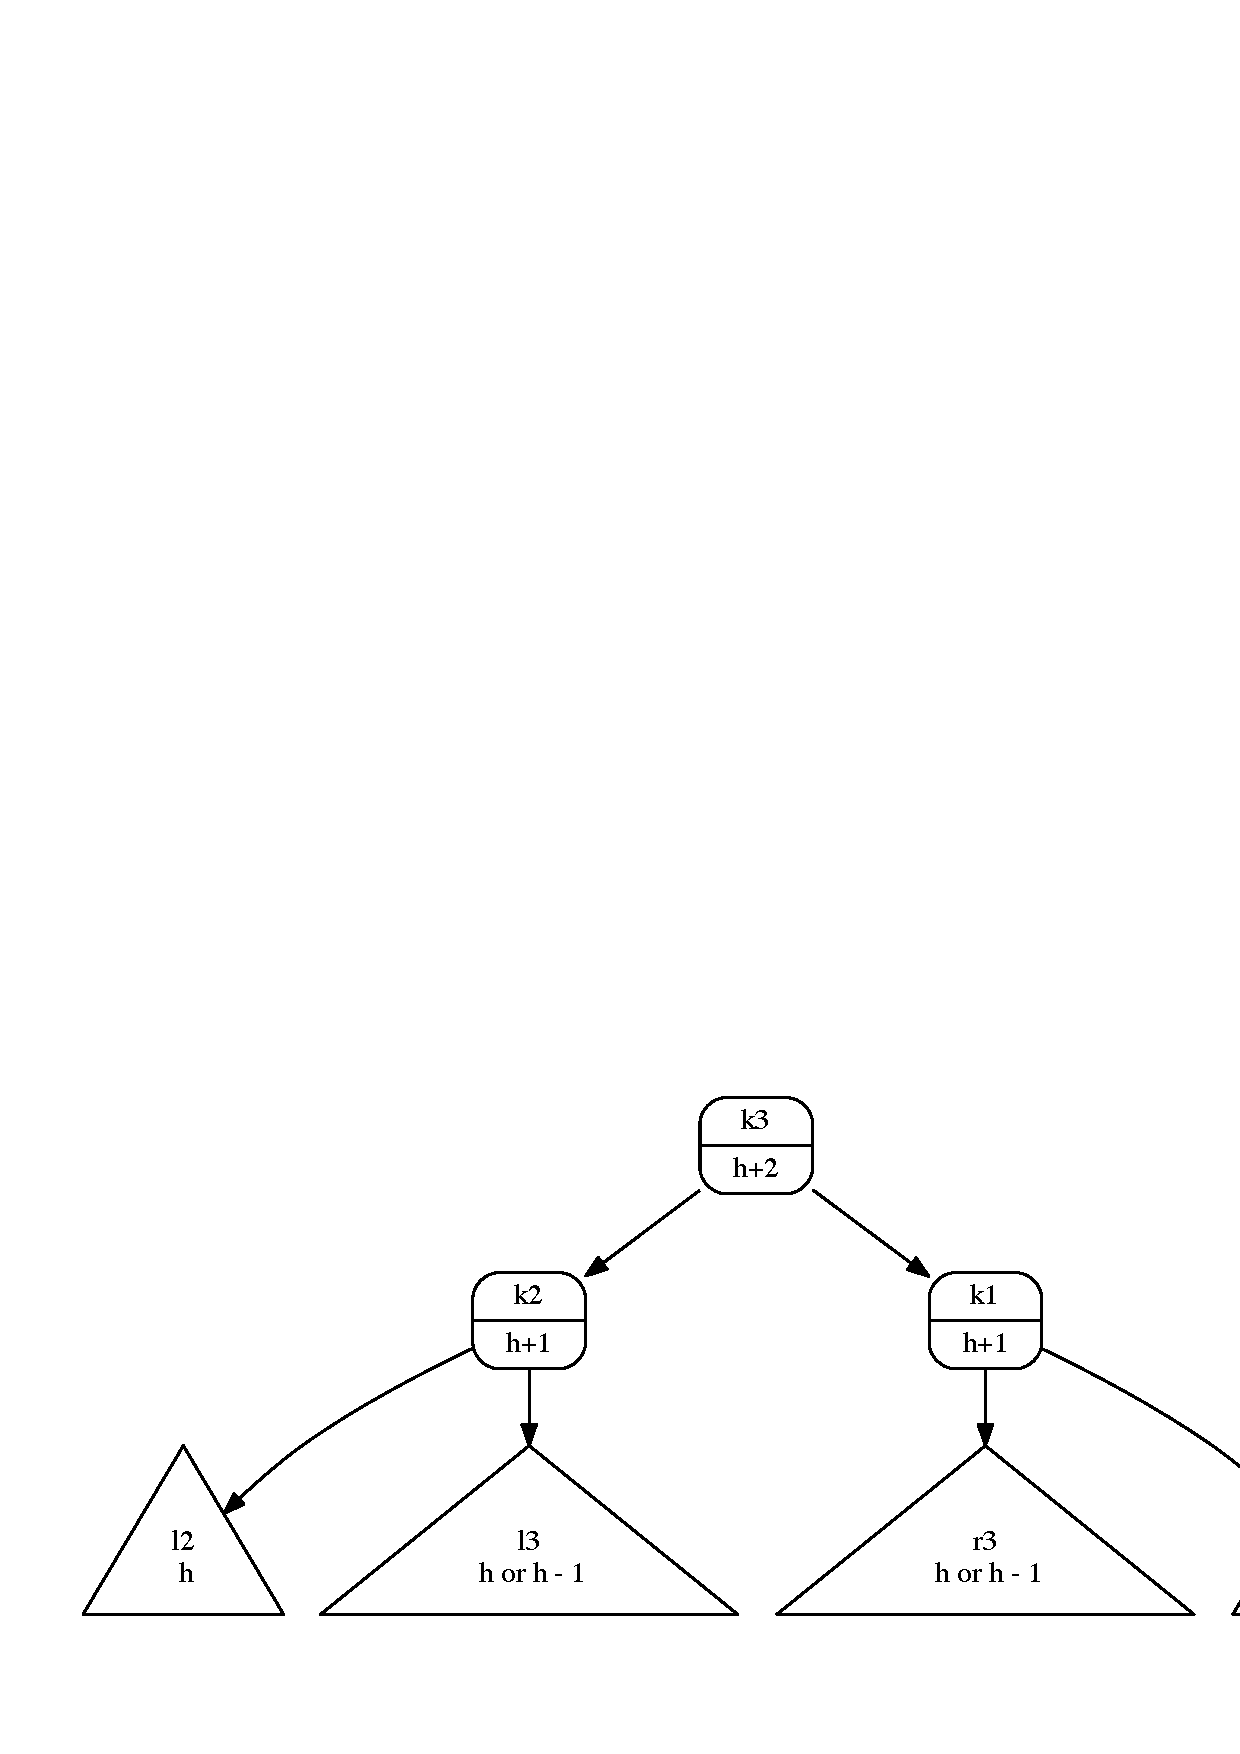
\epsfig{file=caselr-nach,scale=0.7}} 
  \caption{Der rebalancierte Baum im 2. Fall}
  \label{fig:caselr-nach}
\end{figure}

      Die Ungleichung, die die Anordnung der Schl�ssel sowohl im linken als auch rechten
      Baum wieder gibt, lautet\\[0.2cm]
      \hspace*{1.3cm} $l_2 < k_2 < l_3 < k_3 < r_3 < k_1 < r_1$.

      Es gibt noch zwei weitere F�lle die auftreten, wenn der rechte Teilbaum um mehr als
      Eins gr��er ist als der linke Teilbaum.  Diese beiden F�lle sind aber zu den beiden
      vorherigen F�llen v�llig analog, so dass wir die Gleichungen hier ohne weitere
      Diskussion angeben.
\item $\begin{array}[t]{cl}
              & r_1.\textsl{height}() = l_1.\textsl{height}() + 2    \\ 
       \wedge & r_1 = \textsl{Node}(k_2,v_2,l_2,r_2)               \\
       \wedge & r_2.\textsl{height}() \geq l_2.\textsl{height}()     \\[0.2cm]
       \rightarrow & \textsl{Node}(k_1,v_1,l_1,r_1).\textsl{restore}() = 
                     \textsl{Node}\bigl(k_2,v_2,\textsl{Node}(k_1,v_1,l_1,l_2),r_2\bigr)
       \end{array}
      $
\item $\begin{array}[t]{cl}
               & r_1.\textsl{height}() = l_1.\textsl{height}() + 2    \\ 
        \wedge & r_1 = \textsl{Node}(k_2,v_2,l_2,r_2)               \\
        \wedge & r_2.\textsl{height}() < l_2.\textsl{height}()     \\
        \wedge & l_2 = \textsl{Node}(k_3,v_3,l_3,r_3)               \\
        \rightarrow & \textsl{Node}(k_1,v_1,l_1,r_1).\textsl{restore}() = 
                      \textsl{Node}\bigl(k_3,v_3,\textsl{Node}(k_1,v_1,l_1,l_3),\textsl{Node}(k_2,v_2,r_3,r_2) \bigr)
        \end{array}
       $

\end{enumerate}
Damit k�nnen wir nun die Methode $\textsl{insert}()$ durch bedingte rekursive Gleichungen 
beschreiben.  Dabei m�ssen wir die urspr�nglich f�r geordnete B�ume angegebene Gleichungen
dann �ndern, wenn die Balancierungs-Bedingung durch das Einf�gen eines neuen Elements
verletzt werden kann.
\begin{enumerate}
\item $\textsl{Nil}.\textsl{insert}(k,v) = \textsl{Node}(k,v, \textsl{Nil}, \textsl{Nil})$.  
\item $\textsl{Node}(k, v_2, l, r).\textsl{insert}(k,v_1) = \textsl{Node}(k, v_1, l, r)$.
\item $k_1 < k_2 \rightarrow 
          \textsl{Node}(k_2, v_2, l, r).\textsl{insert}(k_1, v_1) =
          \textsl{Node}\bigl(k_2, v_2, l.\textsl{insert}(k_1,v_1), r\bigr).\textsl{restore}()$.
\item $k_1 > k_2 \rightarrow 
         \textsl{Node}(k_2, v_2, l, r).\textsl{insert}\bigl(k_1, v_1\bigr) = 
         \textsl{Node}\bigl(k_2, v_2, l, r.\textsl{insert}(k_1,v_1)\bigr).\textsl{restore}()$.
\end{enumerate}
Analog �ndern sich die Gleichungen f�r $\textsl{delMin}()$ wie folgt:
\begin{enumerate}
\item $\textsl{Node}(k, v, \textsl{Nil}, r).\textsl{delMin}() = \langle r, k, v \rangle$.
\item $l\not= \textsl{Nil} \wedge \langle l',k_{min}, v_{min}\rangle := l.\textsl{delMin}() 
       \;\rightarrow$ \\[0.2cm]
       \hspace*{1.3cm} 
       $\textsl{Node}(k, v, l, r).\textsl{delMin}() = 
        \langle \textsl{Node}(k, v, l', r).\textsl{restore}(), k_{min}, v_{min} \rangle$.
\end{enumerate}
Damit k�nnen wir die Gleichungen zur Spezifikation der  Methode $\mathtt{delete}()$ angeben.
\begin{enumerate}
\item $\textsl{Nil}.\textsl{delete}(k) = \textsl{Nil}$.
\item $\textsl{Node}(k,v,\textsl{Nil},r).\textsl{delete}(k) = r$.
\item $\textsl{Node}(k,v,l,\textsl{Nil}).\textsl{delete}(k) = l$.
\item $l \not= \textsl{Nil} \,\wedge\, r \not= \textsl{Nil} \,\wedge\, 
       \langle r',k_{min}, v_{min} \rangle := r.\textsl{delMin}()  \;\rightarrow$ \\[0.2cm]
      \hspace*{1.3cm}
      $\textsl{Node}(k,v,l,r).\textsl{delete}(k) = \textsl{Node}(k_{min},v_{min},l,r').\textsl{restore}()$.
\item $k_1 < k_2 \rightarrow \textsl{Node}(k_2,v_2,l,r).\textsl{delete}(k_1) = 
       \textsl{Node}\bigl(k_2,v_2,l.\textsl{delete}(k_1),r\bigr).\textsl{restore}()$.
\item $k_1 > k_2 \rightarrow \textsl{Node}(k_2,v_2,l,r).\textsl{delete}(k_1) = 
         \textsl{Node}\bigl(k_2,v_2,l,r.\textsl{delete}(k_1)\bigr).\textsl{restore}()$.
\end{enumerate}
\pagebreak

\subsection{Implementing AVL-Trees in \textsc{SetlX}}
If we want to implement AVL-trees in \textsc{SetlX} then we have to decide how to compute the height
of the trees.  The idea is to store the height of every subtree in the corresponding node since it
would be inefficient if we would recompute this height every time we need it.  Therefore, we add a
member variable \texttt{mHeight} to our class map.
Figure \ref{fig:avl-tree.stlx:outline} shows an outline of the class \texttt{map}.  The variable
\texttt{mHeight} is defined in line 6.  It is initialised as $0$ since the constructor \texttt{map}
constructs an empty node.  

\begin{figure}[!ht]
  \centering
\begin{Verbatim}[ frame         = lines, 
                  framesep      = 0.3cm, 
                  labelposition = bottomline,
                  numbers       = left,
                  numbersep     = -0.2cm,
                  xleftmargin   = 0.0cm,
                  xrightmargin  = 0.0cm
                ]
    class map(cmp) {
        mKey    := om;
        mValue  := om; 
        mLeft   := om;
        mRight  := om;
        mHeight := 0;
        mCmpFct := cmp;  
    
      static {
        isEmpty       := [] |-> mKey == om;
        find          := procedure(k)          { ... };
        insert        := procedure(k, v)       { ... };
        delMin        := procedure()           { ... };
        delete        := procedure(k)          { ... };
        update        := procedure(t)          { ... };
        restore       := procedure()           { ... };
        setValues     := procedure(k, v, l, r) { ... };
        restoreHeight := procedure()           { ... };
      }
    }
\end{Verbatim}
\vspace*{-0.3cm}
  \caption{Outline of the class \texttt{map}.}
  \label{fig:avl-tree.stlx:outline}
\end{figure}


Figure \ref{fig:avl-tree.stlx:find} show the implementation of the function \texttt{find}.
Actually, the implementation is the same as the implementation in Figure
\ref{fig:binary-tree.stlx-1}.  The reason is that every AVL tree is also an ordered binary tree and
since searching for a key does not change the underlying tree there is no need to restore anything.

\begin{figure}[!ht]
\centering
\begin{Verbatim}[ frame         = lines, 
                  framesep      = 0.3cm, 
                  firstnumber   = 1,
                  labelposition = bottomline,
                  numbers       = left,
                  numbersep     = -0.2cm,
                  xleftmargin   = 0.8cm,
                  xrightmargin  = 0.8cm,
                ]
    find := procedure(k) {
        if      (isEmpty())        { return;                }
        else if (mKey == k)        { return mValue;         }
        else if (mCmpFct(k, mKey)) { return mLeft .find(k); }
        else                       { return mRight.find(k); }
    };
\end{Verbatim}
\vspace*{-0.3cm}
\caption{Implementation of the method \texttt{find}.}
\label{fig:avl-tree.stlx:find}
\end{figure}
\pagebreak

Figure \ref{fig:avl-tree.stlx:insert} shows the implementation of the method \texttt{insert}.
If we compare this implementation with the implementation for binary trees, we find three
differences.
\begin{enumerate}
\item When inserting into an empty tree, we now have to update the member variable \texttt{mHeight}
      to $1$.  This is done in line 7.
\item After inserting a value into the left subtree \texttt{mLeft}, it might be necessary to 
      rebalance the tree.  This is done in line 12.
\item Similarly, if we insert a value into the right subtree \texttt{mRight}, we have to rebalance 
      the tree.  This is done in line 15.
\end{enumerate}

\begin{figure}[!ht]
\centering
\begin{Verbatim}[ frame         = lines, 
                  framesep      = 0.3cm, 
                  firstnumber   = 1,
                  labelposition = bottomline,
                  numbers       = left,
                  numbersep     = -0.2cm,
                  xleftmargin   = 0.8cm,
                  xrightmargin  = 0.8cm,
                ]
    insert := procedure(k, v) {
        if (isEmpty()) { 
            this.mKey    := k;
            this.mValue  := v; 
            this.mLeft   := map(mCmpFct);
            this.mRight  := map(mCmpFct);
            this.mHeight := 1;
        } else if (mKey == k) { 
            this.mValue := v; 
        } else if (mCmpFct(k, mKey)) { 
            mLeft.insert(k, v); 
            restore();
        } else { 
            mRight.insert(k, v); 
            restore();
        }
    };
\end{Verbatim}
\vspace*{-0.3cm}
\caption{Implementation of the method \texttt{insert}.}
\label{fig:avl-tree.stlx:insert}
\end{figure}

Figure \ref{fig:avl-tree.stlx:delMin} shows the implementation of the method \texttt{delMin}.
The only change compared to the previous implementation for ordered binary trees is in line 7, where
we have to take care of the fact that the balancing condition might be violated after deleting the
smallest element in the left subtree.

\begin{figure}[!ht]
\centering
\begin{Verbatim}[ frame         = lines, 
                  framesep      = 0.3cm, 
                  firstnumber   = 1,
                  labelposition = bottomline,
                  numbers       = left,
                  numbersep     = -0.2cm,
                  xleftmargin   = 0.8cm,
                  xrightmargin  = 0.8cm,
                ]
    delMin := procedure() {
        if (mLeft.isEmpty()) { 
            return [ mRight, mKey, mValue ]; 
        } else {
             [ ls, km, vm ] := mLeft.delMin();
             this.mLeft := ls;
             restore();
             return [ this, km, vm ];
        }
    };
\end{Verbatim}
\vspace*{-0.3cm}
\caption{Implementation of \texttt{delMin}.}
\label{fig:avl-tree.stlx:delMin}
\end{figure}

\pagebreak
Figure \ref{fig:avl-tree.stlx:delete} shows the implementation of the method \texttt{delete} and the
implementation of the auxiliary method \texttt{update}.  Compared with Figure
\ref{fig:binary-tree.stlx-2} there are only three differences:
\begin{enumerate}
\item If we delete the key at the root of the tree, we replace this key with the smallest key in the
      right subtree.  Since this key is deleted in the right subtree, the height of the right
      subtree might shrunk and hence the balancing condition at the root might be violated.
      Therefore, we have to restore the balancing condition.  This is done in line 12.
\item If we delete a key in the left subtree, the height of the left subtree might shrink.
      Hence we have to rebalance the tree at the root in line 16.
\item Similarly, if we delete a key in the right subtree, we have to restore the balancing
      condition.  This is done in line 19.
\end{enumerate}
Of course, since the method \texttt{update} only sets the member variables of the tree, it does not
change the structure of the tree.  Hence there is no need for a call to \texttt{restore} in this method.

\begin{figure}[!ht]
\centering
\begin{Verbatim}[ frame         = lines, 
                  framesep      = 0.3cm, 
                  firstnumber   = 1,
                  labelposition = bottomline,
                  numbers       = left,
                  numbersep     = -0.2cm,
                  xleftmargin   = 0.0cm,
                  xrightmargin  = 0.0cm,
                ]
    delete := procedure(k) {
        if (isEmpty())  { 
            return; 
        } else if (k == mKey) {
            if (mLeft.isEmpty()) {
                update(mRight);
            } else if (mRight.isEmpty()) {
                update(mLeft);
            } else {
                [ rs, km, vm ] := mRight.delMin();
                [this.mKey,this.mValue,this.mRight ] := [km,vm,rs];
                restore();
            }
        } else if (mCmpFct(k, mKey)) {
            mLeft.delete(k);
            restore();
        } else {
            mRight.delete(k);
            restore();
        }
    };
    update := procedure(t) {
        this.mKey    := t.mKey;
        this.mValue  := t.mValue;
        this.mLeft   := t.mLeft;
        this.mRight  := t.mRight;
        this.mHeight := t.mHeight;
    };
\end{Verbatim}
\vspace*{-0.3cm}
\caption{The methods \texttt{delete} and \texttt{update}.}
\label{fig:avl-tree.stlx:delete}
\end{figure}
\begin{figure}[!ht]
\centering
\begin{Verbatim}[ frame         = lines, 
                  framesep      = 0.3cm, 
                  firstnumber   = 1,
                  labelposition = bottomline,
                  numbers       = left,
                  numbersep     = -0.2cm,
                  xleftmargin   = 0.0cm,
                  xrightmargin  = 0.0cm,
                ]
    restore := procedure() {
        if (abs(mLeft.mHeight - mRight.mHeight) <= 1) {
            restoreHeight();
            return;
        }
        if (mLeft.mHeight > mRight.mHeight) {
            [ k1,v1,l1,r1 ] := [ mKey,mValue,mLeft,mRight ];
            [ k2,v2,l2,r2 ] := [ l1.mKey,l1.mValue,l1.mLeft,l1.mRight ];
            if (l2.mHeight >= r2.mHeight) {
                setValues(k2,v2,l2,createNode(k1,v1,r2,r1,mCmpFct));
            } else {
                [ k3,v3,l3,r3 ] := [r2.mKey,r2.mValue,r2.mLeft,r2.mRight];
                setValues(k3,v3,createNode(k2,v2,l2,l3,mCmpFct),
                                createNode(k1,v1,r3,r1,mCmpFct) );
            }
        }
        if (mRight.mHeight > mLeft.mHeight) {
            [ k1,v1,l1,r1 ] := [ mKey,mValue,mLeft,mRight ];
            [ k2,v2,l2,r2 ] := [ r1.mKey,r1.mValue,r1.mLeft,r1.mRight ];
            if (r2.mHeight >= l2.mHeight) {
                setValues(k2,v2,createNode(k1,v1,l1,l2,mCmpFct),r2);
            } else {
                [ k3,v3,l3,r3 ] := [l2.mKey,l2.mValue,l2.mLeft,l2.mRight];
                setValues(k3,v3,createNode(k1,v1,l1,l3,mCmpFct),
                                createNode(k2,v2,r3,r2,mCmpFct) );
            }
        }
        restoreHeight();
    };
    setValues := procedure(k, v, l, r) {
        this.mKey   := k;
        this.mValue := v;
        this.mLeft  := l;
        this.mRight := r;
    };
    restoreHeight := procedure() {
        this.mHeight := 1 + max({ mLeft.mHeight, mRight.mHeight });
    };
\end{Verbatim}
\vspace*{-0.3cm}
\caption{The implementation of \texttt{restore} and \texttt{restoreHeight}.}
\label{fig:avl-tree.stlx:restore}
\end{figure}

\pagebreak
Figure \ref{fig:avl-tree.stlx:restore} shows the implementation of the function \texttt{restore}.
It is this method that makes most of the difference between ordered binary trees and AVL trees.  Let
us discuss this method line by line.
\begin{enumerate}
\item In line 2 we check whether the balancing condition is satisfied.  If we are lucky,  this test 
      is successful and hence we do not need to restore the structure of the tree.  However, we
      still need to maintain the height of the tree since it is possible that variable
      \texttt{mHeight} no longer contains the correct height.  For example, assume that the left subtree
      initially has a height that is bigger by one than the height of the right subtree.  Assume
      further that we have deleted a node in the left subtree so that its height shrinks.  Then the
      balancing condition is still satisfied, as now the left subtree and the right subtree have the
      same height.  However, the height of the complete tree has also shrunk by one and therefore, 
      the variable \texttt{mHeight} needs to be decremented.  This is done via the auxiliary method
      \texttt{restoreHeight}.  This method is defined in line 36 and it recomputes \texttt{mHeight}
      according to the definition of the height of a binary tree.
\item If the check in line 2 fails, then we know that the balancing condition is violated.
      However, we do not yet know which of the two subtrees is bigger.  

      If the test in line 6 succeeds, then the left subtree must have a height that is bigger by
      two than the height of the right subtree.  In order to be able to use the same variable names 
      as the variable names given in the equations discussed in the previous subsection, we define
      the variables \texttt{k1}, \texttt{v1}, $\cdots$, \texttt{l2}, and \texttt{r2} in line 7 and 8
      so that these variable names correspond exactly to the variable names used in the Figures
      \ref{fig:casell} and \ref{fig:caselr}.
\item Next, the test in line 9 checks whether we have the case that is depicted in Figure
      \ref{fig:casell}.  In this case, Figure \ref{fig:casell} tells us that the key \texttt{k2}
      has to move to the root.  The left subtree is now \texttt{l2}, while the right subtree is a
      new node that has the key \texttt{k1} at its root.  This new node is created by the call
      of the function \texttt{createNode} in line 10.  The function \texttt{createNode} is shown in
      Figure \ref{fig:avl-tree.stlx:createNode} on page \pageref{fig:avl-tree.stlx:createNode}.
\item If the test in line 9 fails, the right subtree is bigger than the left subtree and we are in 
      the case that is depicted in Figure \ref{fig:caselr}.  We have to create the tree that is
      shown in Figure \ref{fig:caselr-nach}.  To this end we first define the variables 
      \texttt{k3}, \texttt{v3}, \texttt{l3}, and \texttt{r3} in a way that these variables
      correspond to the variables shown in Figure \ref{fig:caselr}.  Next, we create the tree
      that is shown in Figure \ref{fig:caselr-nach}.
\item Line 17 deals with the case that the right subtree is bigger than the left subtree. 
      As this case is analogous to the case covered in line 6 to line 16, we won't discuss this case
      any further.
\item Finally, we recompute the variable \texttt{mHeight} since it is possible that the old value is
      no longer correct.
\end{enumerate}


\begin{figure}[!ht]
\centering
\begin{Verbatim}[ frame         = lines, 
                  framesep      = 0.3cm, 
                  firstnumber   = 1,
                  labelposition = bottomline,
                  numbers       = left,
                  numbersep     = -0.2cm,
                  xleftmargin   = 0.8cm,
                  xrightmargin  = 0.8cm,
                ]
    createNode :=  procedure(key, value, left, right, cmp) {
        node         := map(cmp);
        node.mKey    := key;
        node.mValue  := value;
        node.mLeft   := left;
        node.mRight  := right;
        node.mCmpFct := cmp;
        node.mHeight := 1 + max({ left.mHeight, right.mHeight });
        return node;
    };
\end{Verbatim}
\vspace*{-0.3cm}
\caption{}
\label{fig:avl-tree.stlx:createNode}
\end{figure}

The function \texttt{createNode} shown in Figure \ref{fig:avl-tree.stlx:createNode}
constructs a node with given left and right subtrees.  In fact, this method serves as a second
constructor for the class \texttt{map}.  The implementation should be obvious.


\subsection{Analyse der Komplexit�t}
Wir analysieren jetzt die Komplexit�t von AVL-B�umen im schlechtesten Fall. Der
schlechteste Fall tritt dann ein, wenn bei einer vorgegebenen Zahl von Schl�sseln die H�he
maximal wird.  Das ist aber dasselbe wie wenn in einem Baum gegebener H�he die Zahl der
Schl�ssel minimal wird.  Wir definieren daher $b_h(k)$ als einen AVL-Baum der H�he $h$, der
unter allen AVL-B�umen der H�he $h$ die minimale Anzahl von Schl�sseln hat.  Au�erdem
sollen alle Schl�ssel, die in $b_h(k)$ auftreten, gr��er als der Schl�ssel $k$ sein.
Sowohl die Schl�ssel als auch die Werte sind in diesem Zusammenhang eigentlich unwichtig,
wir m�ssen nur darauf achten, dass die Ordnungs-Bedingung f�r bin�re B�ume erf�llt ist.
Wir werden f�r die Schl�ssel nat�rliche Zahlen nehmen, f�r die Werte nehmen wir immer die
Zahl $0$.  Bevor wir mit der Definition von $b_h(k)$ beginnen k�nnen, ben�tigen wir noch eine
Hilfs-Funktion $\textsl{maxKey}()$ mit der Signatur  
\[ \textsl{maxKey}:\mathcal{B}_< \rightarrow \textsl{Key} \]
F�r einen gegebenen geordneten nicht-leeren bin�ren Baum $b$ 
berechnet $b.\textsl{maxKey}()$ den gr��ten Schl�ssel, der in $b$ auftritt.  Die
Definition von $b.\textsl{maxKey}()$ ist induktiv:
\begin{enumerate}
\item $\textsl{Node}(k,v,l,\textsl{Nil}).\textsl{maxKey}() = k$,
\item $r \not= \textsl{Nil} \rightarrow \textsl{Node}(k,v,l,r).\textsl{maxKey}() = r.\textsl{maxKey}()$.
\end{enumerate}
Damit k�nnen wir nun die B�ume $b_h(k)$ durch Induktion nach der H�he $h$ definieren.
\begin{enumerate}
\item $b_0(k) = Nil$,

      denn es gibt genau einen AVL-Baum der H�he $0$ und dieser enth�lt keinen Schl�ssel.
\item $b_1(k) = \textsl{Node}(k+1,0,\textsl{Nil}, \textsl{Nil})$,

      denn es gibt genau einen AVL-Baum der H�he $1$.
\item $b_{h+1}(k).\textsl{maxKey}() = l \rightarrow 
       b_{h+2}(k) = \textsl{Node}\bigl(l+1,\,0,\,b_{h+1}(k),\,b_h(l+1)\bigr)$,

      denn um einen AVL-Baum der H�he $h+2$ mit einer minimalen Anzahl an Schl�sseln zu
      konstruieren, erzeugen wir zun�chst den AVL-Baum $b_{h+1}(k)$ der H�he $h+1$.
      Dann bestimmen wir den maximalen Schl�ssel $l$ in diesem Baum, der Schl�ssel $l+1$
      kommt nun an die Wurzel des zu erzeugenden Baums der H�he $h+2$ und schlie�lich erzeugen wir noch
      den Baum $b_h(l+1)$ der H�he $h$, den wir als rechten Teilbaum in den neu zu
      erzeugenden Baum der H�he $h+2$  einf�gen.
\end{enumerate}
F�r einen beliebigen bin�ren Baum $b$ bezeichne $\#\,b$ die Anzahl der Schl�ssel, die in
$b$ auftreten.  Dann definieren wir 
\\[0.2cm]
\hspace*{1.3cm}
$c_h := \#\, b_h(k)$
\\[0.2cm]
als die Anzahl der Schl�ssel des Baums $b_h(k)$.  Wir werden sofort sehen, dass
$\#\,b_h(k)$ nicht von $k$ abh�ngt.  F�r $c_h$ finden wir in Analogie zu
der induktiven Definition von $b_h(k)$ die folgenden Gleichungen.
\begin{enumerate}
\item $c_0 = \#\, b_0(k) = \#\, \textsl{Nil} = 0$,
\item $c_1 = \#\, b_1(k) = \#\, \textsl{Node}(k+1,0,\textsl{Nil}, \textsl{Nil}) = 1$, 
\item$\begin{array}[t]{lcl}
       c_{h+2} & = & \#\, b_{h+2}(k) \\
               & = & \#\,\textsl{Node}\bigl(l+1,\,0,\,b_{h+1}(k),\,b_h(l+1)\bigr) \\
               & = & \#\, b_{h+1}(k) + \#\, b_h(l+1) + 1 \\
               & = & c_{h+1} + c_h + 1.
       \end{array}$
\end{enumerate}
Also haben wir zur Bestimmung von $c_h$ die Rekurrenz-Gleichung
\\[0.2cm]
\hspace*{1.3cm}
$c_{h+2} = c_{h+1} + c_h + 1 \quad \mbox{mit den Anfangs-Bedingungen $c_0 = 0$ und $c_1 = 1$}$
\\[0.2cm]
zu l�sen.  Das ist eine Rekurrenz-Gleichung,
die wir, allerdings mit leicht ver�nderten Anfangs-Bedingungen, bereits im dritten Kapitel gel�st haben.
Sie k�nnen leicht nachrechnen, dass die L�sung dieser Rekurrenz-Gleichung wie folgt
lautet: 
\\[0.2cm]
\hspace*{1.3cm}
$c_h = \displaystyle \frac{1}{\sqrt{5}} \left( \lambda_1^{h+2} - \lambda_2^{h+2} \right) -
1$  \quad mit
\\[0.2cm]
\hspace*{1.3cm}
$\lambda_1 = \displaystyle \frac{1}{2}(1 + \sqrt{5}) \approx  1.618034$ \quad und \quad $\lambda_2 =
\displaystyle \frac{1}{2}(1 - \sqrt{5}) \approx -0.618034$.
\\[0.2cm]
Da $|\lambda_2| < 1$ ist, spielt der Wert $\displaystyle\lambda_2^{h+2}$
f�r gro�e Werte von $h$   praktisch keine Rolle und die
minimale Zahl $n$ der Schl�ssel in einem Baum der H�he $h$ ist durch \\[0.2cm]
\hspace*{1.3cm} $n \approx \displaystyle \frac{1}{\sqrt{5}} \lambda_1^{h+2} - 1$ \\[0.2cm]
gegeben.  Um diese Gleichung nach $h$ aufzul�sen, bilden wir auf beiden Seiten den
Logarithmus zur Basis 2.  Dann erhalten wir 
\\[0.2cm]
\hspace*{1.3cm}
$\log_2(n+1) = (h+2) \cdot \log_2(\lambda_1) - \frac{1}{2}\cdot \log_2(5)$
\\[0.2cm]
Daraus folgt nach Addition von $\frac{1}{2}\cdot \log_2(5)$
\\[0.2cm]
\hspace*{1.3cm}
$\log_2(n+1) + \frac{1}{2}\cdot \log_2(5) = (h+2) \cdot \log_2(\lambda_1)$
\\[0.2cm]
Jetzt teilen wir durch $\log_2(\lambda_1)$.  Dann erhalten wir 
\\[0.4cm]
\hspace*{1.3cm}
$\displaystyle \bruch{\log_2(n+1) + \frac{1}{2}\cdot \log_2(5)}{\log_2(\lambda_1)} = h+2$
\\[0.2cm]
L�sen wir diese Gleichung nach $h$ auf, so haben wir f�r gro�e $n$
das Ergebnis
\\[0.4cm]
\hspace*{1.3cm} 
$
\begin{array}[t]{lcl}
h & = & \displaystyle \bruch{\log_2(n+1) + \frac{1}{2}\cdot \log_2(5)}{\log_2(\lambda_1)} - 2 \\[0.4cm]
  & = & \bruch{1}{\log_2(\lambda_1)}\cdot \log_2(n) + \Oh(1) \\[0.5cm]
  & \approx & 1,44 \cdot \log_2(n) + \Oh(1)
\end{array} 
$
\\[0.2cm]
gewonnen. 
Die Gr��e $h$ gibt aber die Zahl der Vergleiche an, die wir im ung�nstigsten Fall bei
einem Aufruf von \textsl{find} in einem AVL-Baum mit $n$ Schl�sseln durchf�hren m�ssen.
Wir sehen also, dass bei einem AVL-Baum auch im schlechtesten Fall die Komplexit�t
logarithmisch bleibt.  Abbildung
\ref{fig:avl-worst-case} zeigt einen AVL-Baum der H�he 6, f�r den das Verh�ltnis von H�he zur Anzahl
der Knoten maximal wird.  Wie man sieht ist auch dieser Baum noch sehr weit weg von dem
zur Liste entarteten Baum aus der Abbildung \ref{fig:degenerated}.


\begin{figure}[!ht]
  \centering
  \framebox{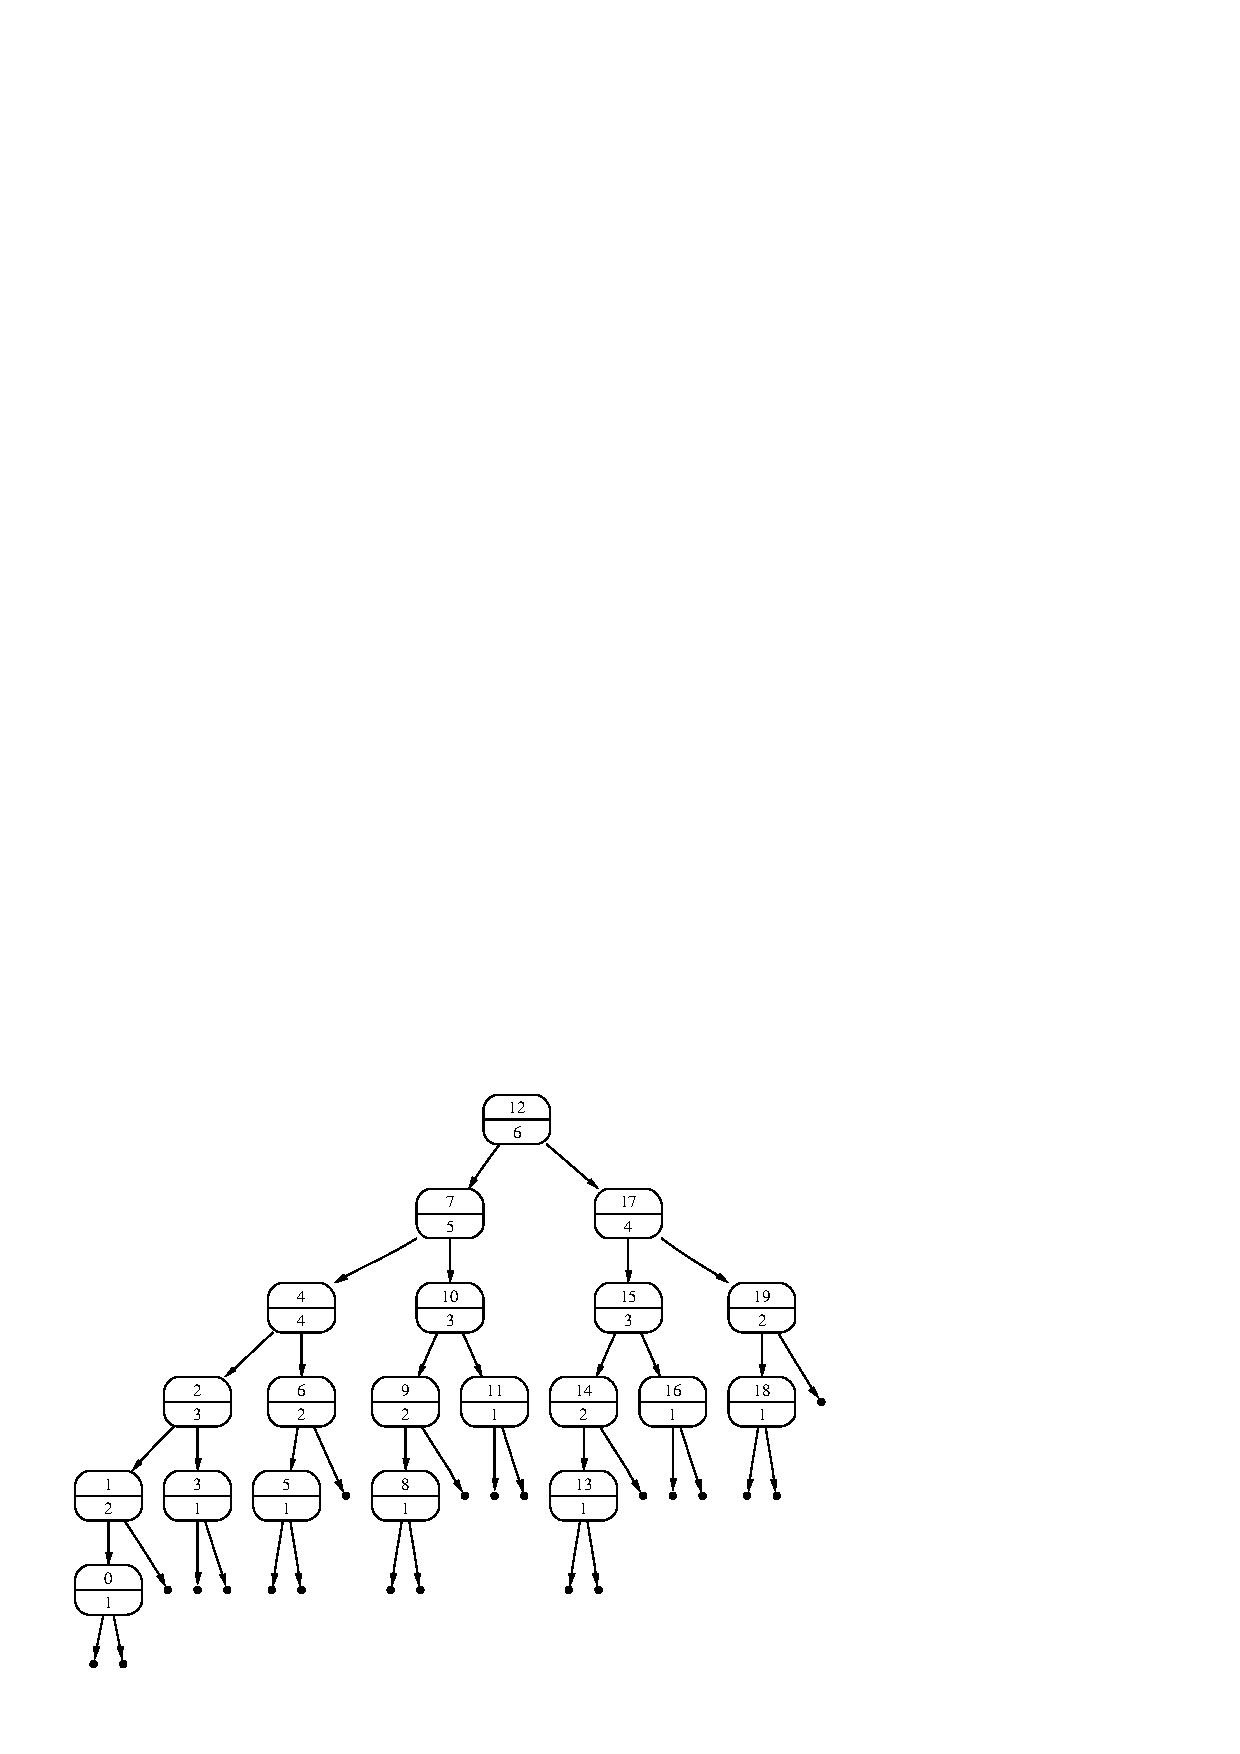
\epsfig{file=avl}} 
  \caption{Ein AVL-Baum mit dem ung�nstigsten Verh�ltnis von H�he zur Anzahl an Knoten}
  \label{fig:avl-worst-case}
\end{figure}

\subsection{Further Reading}
In practice, \emph{red-black trees} are slightly faster than \textsl{Avl} trees.  Similar to
\textsl{Avl} trees, a  red-black
  is an ordered binary tree that is approximately balanced.  Nodes are either black or red.
The children of a red tree have to be black.  In order to keep red-black trees approximately
balanced, a \emph{relaxed height} of a tree is defined.  Red nodes do not contribute to the relaxed
height of a tree.  The left and right subtree of a red-black tree are required to have the same 
relaxed height.  A detailed and very readable exposition of red-black trees is given in \cite{sedgewick:2011}.



\section{Tries}
In der Praxis kommt es h�ufig vor, dass die Schl�ssel des ADT \textsl{Map} Strings sind.
In dem einf�hrenden Beispiel des elektronischen Telefon-Buchs ist dies der Fall.  Es gibt eine
Form von Such-B�umen, die auf diese Situation besonders angepasst ist.  Diese Such-B�ume
haben den Namen \emph{Tries}.  Dieses Wort ist von dem Englischen Wort
\emph{re\underline{trie}val} abgeleitet. Damit man \emph{Tries} und \emph{Trees}
unterscheiden kann, wird \emph{Trie} so ausgesprochen, dass es sich mit dem Englischen
Wort \emph{pie} reimt.  Diese Datenstruktur wurde 1959 von Ren\'e de la Briandais
\cite{briandais:59} vorgeschlagen.


Die Grundidee bei der Datenstruktur \emph{Trie} ist ein Baum, an dem jeder Knoten nicht
nur zwei Nachfolger hat, wie das bei bin�ren B�umen der Fall ist, sondern statt dessen
potentiell f�r jeden Buchstaben des Alphabets einen Ast besitzt.  Um Tries definieren zu
k�nnen, nehmen wir zun�chst an, dass folgendes gegeben ist:
\begin{enumerate}
\item $\Sigma$ ist eine endliche Menge, deren Elemente wir als \emph{Buchstaben}
      bezeichnen. $\Sigma$ selbst hei�t das \emph{Alphabet}.
\item $\Sigma^*$ bezeichnet die Menge der \emph{W�rter} (engl.~\emph{strings}), die wir aus den Buchstaben
      des Alphabets bilden k�nnen.  Mathematisch k�nnen wir W�rter als Listen von 
      Buchstaben auffassen. Ist $w \in \Sigma^*$ so schreiben wir $w = cr$, falls
      $c$ der erste Buchstabe von $w$ ist und $r$ das Wort ist, das durch L�schen des
      ersten Buchstabens aus $w$ entsteht.  
\item $\varepsilon$ bezeichnet das leere Wort.  
\item \textsl{Value} ist eine Menge von \emph{Werten}.  
\end{enumerate}
Die Menge $\mathbb{T}$ der Tries definieren wir nun induktiv mit Hilfe des 
Konstruktors \\[0.2cm]
\hspace*{1.3cm} 
$\texttt{Node}: \textsl{Value} \times \textsl{List}(\Sigma) \times
\textsl{List}(\mathbb{T}) \rightarrow \mathbb{T}$. \\[0.2cm]
Die induktive Definition besteht nur aus einer einzigen Klausel: Falls
\begin{enumerate}
\item $v \in \textsl{Value} \cup \{\Omega\}$
\item $C = [c_1, \cdots, c_n] \in \textsl{List}(\Sigma)$ eine Liste von Buchstaben der
      L�nge $n$ ist,
\item $T = [t_1, \cdots, t_n] \in \textsl{List}(\mathbb{T})$ eine Liste von Tries derselben L�nge $n$ ist, 
\end{enumerate}
dann gilt \\[0.2cm]
\hspace*{1.3cm}  $\texttt{Node}(v, C, T) \in \mathbb{T}$.  \\[0.2cm]
Als erstes fragen Sie sich
vermutlich, wo bei dieser induktiven Definition der Induktions-Anfang ist.
Der Induktions-Anfang ist der Fall $n=0$, denn dann sind die Listen $L$ und $T$ leer.
Als n�chstes �berlegen wir uns, welche Funktion von dem Trie \\[0.2cm]
\hspace*{1.3cm}  $\texttt{Node}(v, [c_1, \cdots, c_n], [t_1, \cdots, t_n]) \in \mathbb{T}$ \\[0.2cm]
dargestellt wird.  Wir beantworten diese Frage, indem wir rekursive Gleichungen f�r die
Methode \\[0.2cm]
\hspace*{1.3cm} $\textsl{find}: \mathbb{T} \times \Sigma^* \rightarrow \textsl{Value} \cup \{ \Omega\}$
\\[0.2cm]
angeben.  Wir werden den Ausdruck $\texttt{Node}(v,L,T).\textsl{find}(s)$ durch
Induktion �ber den String $s$ 
definieren:
\begin{enumerate}
\item $\texttt{Node}(v, C, T).\textsl{find}(\varepsilon) = v$.

      Der dem leeren String zugeordnete Wert wird also unmittelbar an der Wurzel
      des Tries abgespeichert.
\item $\texttt{Node}(v, [c_1, \cdots, c_n], [t_1, \cdots, t_n]).\textsl{find}(cr) = 
        \left\{
        \begin{array}{ll}
        t_1.\textsl{find}(r) & \mbox{falls} \quad c = c_1 \mbox{;} \\
        \vdots &                                     \\
        t_i.\textsl{find}(r) & \mbox{falls} \quad c = c_i \mbox{;} \\
        \vdots &                                     \\
        t_n.\textsl{find}(r) & \mbox{falls} \quad c = c_n \mbox{;} \\[0.2cm]
        \Omega               & \mbox{falls} \quad c \notin \{c_1,\cdots,c_n\} \mbox{.}         
        \end{array}
       \right.$

      Der Trie $\texttt{Node}(v, [c_1, \cdots, c_n], [t_1, \cdots, t_n])$ enth�lt also genau
      dann einen Wert zu dem Schl�ssel $cr$, wenn es in der Liste $[c_1, \cdots, c_n]$
      eine Position $i$ gibt, so dass der Buchstabe $c$ mit dem Buchstaben $c_i$
      �bereinstimmt  wenn au�erdem der Trie $t_i$ einen Wert zu dem
      Schl�ssel $r$ enth�lt.
\end{enumerate}

\begin{figure}[!ht]
  \centering
  \framebox{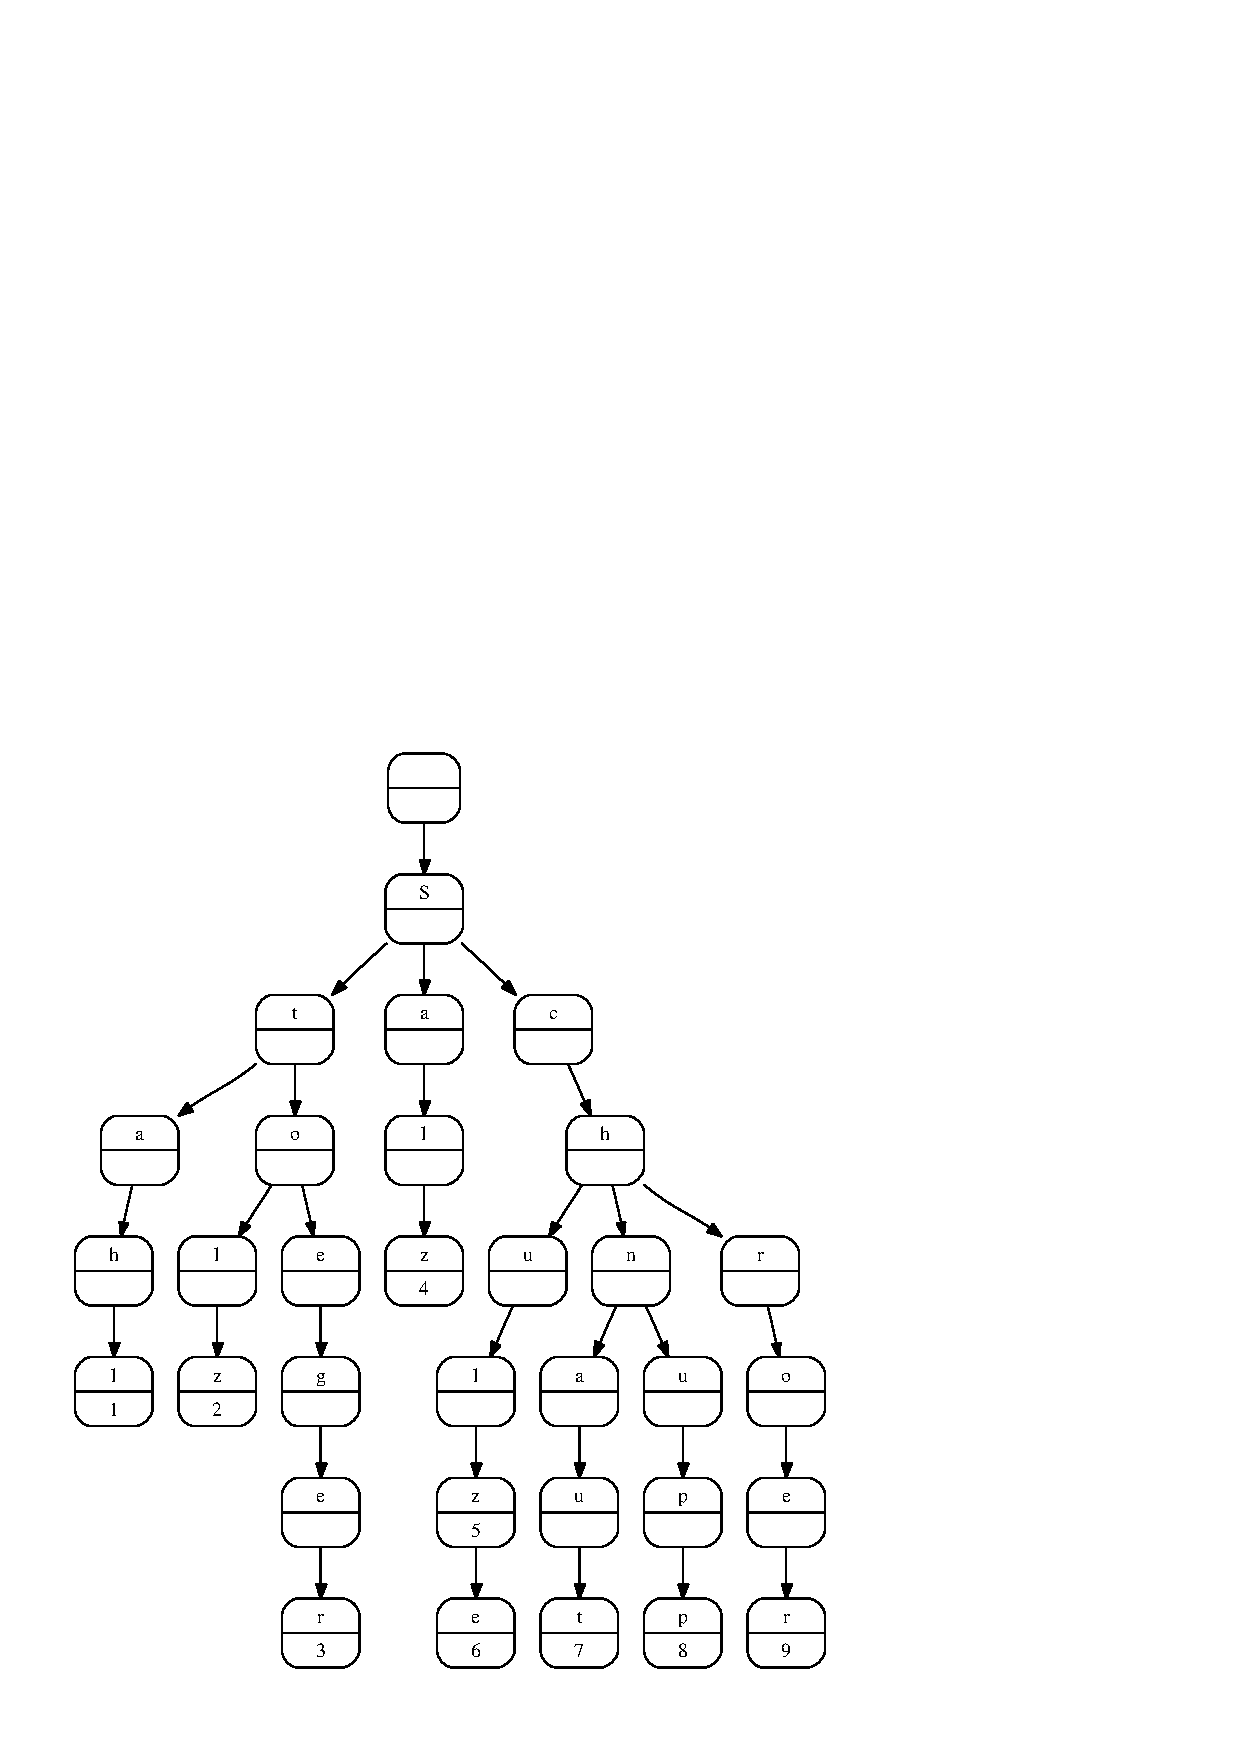
\epsfig{file=trie}} 
  \caption{Ein Beispiel Trie}
  \label{fig:trie}
\end{figure}

Zum besseren Verst�ndnis wollen wir Tries graphisch als B�ume darstellen.
Nun ist es nicht sinnvoll, die Knoten dieser B�ume mit langen Listen zu beschriften.
Wir behelfen uns mit einem Trick.  Um einen Knoten der Form \\[0.2cm]
\hspace*{1.3cm} 
$\texttt{Node}(v, [c_1, \cdots, c_n], [t_1, \cdots, t_n])$ \\[0.2cm]
darzustellen, zeichnen wir einen Kreis,
den wir durch einen horizontalen Strich in der Mitte aufteilen.
Falls $v$ von $\Omega$ verschieden ist, schreiben wir den Wert $v$ in die untere H�lfte
des Kreises.
Das, was wir �ber dem Strich schreiben,
h�ngt von dem Vater des jeweiligen Knotens ab.  Wie genau es vom Vater abh�ngt, sehen wir gleich.
Der Knoten selber hat $n$ Kinder. Diese $n$ Kinder sind die 
Wurzeln der B�ume, die die Tries $t_1$, $\cdots$, $t_n$ darstellen.
Au�erdem markieren wir die diese Knoten darstellenden Kreise in den oberen H�lfte 
mit den Buchstaben $c_1$, $\cdots$, $c_n$.  


Zur Verdeutlichung geben wir ein Beispiel in 
Abbildung \ref{fig:trie} auf Seite \pageref{fig:trie}.
Die Funktion, die hier dargestellt wird, l�sst sich wie folgt als bin�re Relation
schreiben: \\[0.2cm]
\hspace*{1.3cm} $ \bigl\{ \langle \textrm{``Stahl''},   1  \rangle, \langle \textrm{``Stolz''},     2  \rangle, \langle \textrm{``Stoeger''},   3  \rangle, 
             \langle \textrm{``Salz''},      4  \rangle, \langle \textrm{``Schulz''},    5  \rangle$, \\[0.2cm]
\hspace*{1.5cm} $\langle \textrm{``Schulze''},   6  \rangle, \langle \textrm{``Schnaut''},   7  \rangle, 
  \langle \textrm{``Schnupp''},   8  \rangle, 
  \langle \textrm{``Schroer''},   9  \rangle\}$. \\[0.2cm]
Der Wurzel-Knoten ist hier leer, denn dieser Knoten hat keinen Vater-Knoten, von dem er
eine Markierung erben k�nnte.  Diesem Knoten entspricht der Term \\[0.2cm]
\hspace*{1.3cm} $\texttt{Node}(\Omega,[\textrm{`S'}], [t])$. \\[0.2cm]
Dabei bezeichnet $t$ den Trie, dessen Wurzel mit dem Buchstaben `S' markiert ist.
Diesen Trie k�nnen wir seinerseits durch den Term \\[0.2cm]
\hspace*{1.3cm} 
$\texttt{Node}(\Omega,[\textrm{`t'},\textrm{`a'},\textrm{`c'}], [t_1, t_2, t_3])$ \\[0.2cm]
darstellen.  Daher hat dieser Knoten drei S�hne, die mit den Buchstaben `t', `a' und `c'
markiert sind.

\subsection{Einf�gen in Tries}
Wir stellen nun bedingte Gleichungen auf, mit denen wir das Einf�gen eines Schl�ssels mit
einem zugeh�rigen Wert beschreiben k�nnen.  Bezeichnen wir die Methode f�r das Einf�gen
mit $\textsl{insert}()$, so hat diese Methode die Signatur
\\[0.2cm]
\hspace*{1.3cm}
$\textsl{insert}: \mathbb{T} \times \Sigma^* \times V \rightarrow \mathbb{T}$.
\\[0.2cm]
Wir definieren den Wert von \\[0.2cm]
\hspace*{1.3cm} 
$\texttt{Node}(v, [c_1, \cdots, c_n], [t_1, \cdots, t_n]).\textsl{insert}(s,v)$
\\[0.2cm]
f�r ein Wort $w\in \Sigma^*$ und einen Wert $v \in V$
durch Induktion nach der L�nge des Wortes $w$.
\begin{enumerate}
\item $\texttt{Node}(v_1,L,T).\textsl{insert}(\varepsilon, v_2) = \texttt{Node}(v_2,L,T)$,

      Einf�gen eines Wertes mit dem leeren String als Schl�ssel �berschreibt einfach
      den an dem Wurzel-Knoten gespeicherten Wert. 
\item $\texttt{Node}\bigl(v_1,[c_1,\cdots,c_i,\cdots,c_n], [t_1,\cdots,t_i,\cdots,t_n]\bigr).\textsl{insert}(c_ir,v_2) =$ \\[0.2cm]
      \hspace*{1.3cm}  
      $\texttt{Node}\bigl(v_1,[c_1,\cdots,c_i,\cdots,c_n], [t_1,\cdots,t_i.\textsl{insert}(r,v_2),\cdots,t_n]\bigr)$.

      Wenn in dem Trie $\texttt{Node}\bigl(v_1,[c_1,\cdots,c_i,\cdots,c_n], [t_1,\cdots,t_i,\cdots,t_n]\bigr)$ ein Wert
      $v_2$ zu dem Schl�ssel $cr$ eingef�gt werden soll, und falls der Buchstabe $c$ in der Liste $[c_1,\cdots,c_n]$
      an der Stelle $i$ vorkommt, wenn also gilt $c= c_i$, dann muss der Wert $v_2$
      rekursiv in dem Trie $t_i$ unter dem Schl�ssel 
      $r$ eingef�gt werden.

\item $c \not\in\{c_1,\cdots,c_n\} \;\rightarrow\;\texttt{Node}\bigl(v_1,[c_1,\cdots,c_n], [t_1,\cdots,t_n]\bigr).\textsl{insert}(cr,v_2) =$ \\[0.2cm]
      \hspace*{1.3cm}  
      $\texttt{Node}\bigl(v_1,[c_1,\cdots,c_n,c], [t_1,\cdots,t_n,\texttt{Node}(\Omega,[],[]).\textsl{insert}(r,v_2)]\bigr)$.
      
      Wenn in dem Trie $\texttt{Node}\bigl(v_1,[c_1,\cdots,c_n], [t_1,\cdots,t_n]\bigr)$
      ein Wert $v_2$ zu dem Schl�ssel $cr$ eingef�gt werden soll, und falls der Buchstabe
      $c$ in der Liste $[c_1,\cdots,c_n]$ nicht vorkommt, dann wird zun�chst ein Trie
      erzeugt, der die leere Abbildung repr�sentiert.  Dieser Trie hat die Form \\[0.2cm]
      \hspace*{1.3cm} $\texttt{Node}(\Omega, [], [])$. \\[0.2cm]
      Anschlie�end wird in diesem Trie der Wert $v_2$ rekursiv unter dem Schl�ssel $r$
      eingef�gt. Zum Schluss h�ngen wir den Buchstaben $c$ an die Liste $[c_1,\cdots,c_n]$      
      an und f�gen den Trie  \\[0.2cm] 
      \hspace*{1.3cm}
      $\texttt{Node}(\Omega, [], []).\textsl{insert}(r,v_2)$ 
      \\[0.2cm]
      am Ende der Liste $[t_1,\cdots,t_n]$ ein.
\end{enumerate}

\subsection{L�schen in Tries}
Als letztes stellen wir die bedingten Gleichungen auf, die das L�schen von
Schl�sseln und den damit verkn�pften Werten in einem Trie beschreiben.
Um diese Gleichungen einfacher schreiben zu k�nnen, definieren wir zun�chst eine
Hilfs-Funktion 
\\[0.2cm]
\hspace*{1.3cm} 
$\textsl{isEmpty}: \mathbb{T} \rightarrow \mathbb{B}$, 
\\[0.2cm]
so dass $t.\textsl{isEmpty}()$ genau dann $\mathtt{true}$ liefert, wenn der Trie
$t$ die leere Funktion darstellt.  Wir definieren also: 
\begin{enumerate}
\item $\texttt{Node}(\Omega, [],[]).\textsl{isEmpty}() = \mathtt{true}$,
\item $v \not= \Omega \rightarrow 
       \texttt{Node}(v, [c_1,\cdots,c_n],[t_1,\cdots,t_n]).\textsl{isEmpty}() = \mathtt{false}$,
\item $\texttt{Node}(\Omega, L, T).\textsl{isEmpty}() = \textsl{isEmptyList}(T)$
\end{enumerate}
In der letzten Gleichung haben wir eine weitere Hilfs-Funktion benutzt, die wir noch
definieren m�ssen.  Die Funktion
\\[0.2cm]
\hspace*{1.3cm}
$\textsl{isEmptyList}: \textsl{List}(\mathbb{T}) \rightarrow \mathbb{B}$
\\[0.2cm]
pr�ft f�r eine gegebene Liste von Tries, ob alle in der Liste vorhandenen Tries leer sind.
Die Definition dieser Funktion erfolgt durch Induktion �ber die L�nge der Liste.
\begin{enumerate}
\item $\textsl{isEmptyList}\bigl([]\bigr) = \mathtt{true}$,
\item $\textsl{isEmptyList}\bigl([t] + r\bigr) = \bigl(t.\textsl{isEmpty}() \wedge \textsl{isEmptyList}(r)\bigr)$,

      denn alle Tries in der Liste $[t]+r$ sind leer, wenn einerseits $t$ ein leerer
      Trie ist und wenn andererseits auch alle Tries in $r$ leer sind.
\end{enumerate}
Nun k�nnen wir die Methode
\\[0.2cm]
\hspace*{1.3cm}
$\textsl{delete}: \mathbb{T} \times \Sigma^* \rightarrow \mathbb{T}$
\\[0.2cm]
spezifizieren:  Wir definieren den Wert von \\[0.2cm]
\hspace*{1.3cm} 
$t.\textsl{delete}(w)$
\\[0.2cm]
f�r einen Trie $t \in \mathbb{B}$ und ein Wort $w \in \Sigma^*$
durch Induktion nach der L�nge des Wortes $w$.
\begin{enumerate}
\item $\texttt{Node}(v,L,T).\textsl{delete}(\varepsilon) = \texttt{Node}(\Omega,L,T)$,

      denn der Wert, der unter dem leeren String $\varepsilon$ in einem Trie
      gespeichert wird, befindet sich unmittelbar an der Wurzel des Tries und
      kann dort sofort gel�scht werden.
\item $\begin{array}[t]{ll}
       t_i.\textsl{delete}(r).\textsl{isEmpty}()   & \rightarrow \\
       \texttt{Node}(v, [c_1,\cdots,c_i,\cdots,c_n],[t_1,\cdots,t_i,\cdots,t_n]).\textsl{delete}(c_ir) 
       & = \\
       \qquad 
       \texttt{Node}(v, [c_1,\cdots,c_{i-1},c_{i+1},\cdots,c_n],[t_1,\cdots,t_{i-1},t_{i+1},\cdots,t_n]).
       \end{array}
       $

       Wenn der zu l�schende String mit dem Buchstaben $c_i$ anf�ngt, und wenn
       das L�schen des Schl�ssels $r$ in dem $i$-ten Trie $t_i$ einen leeren
       Trie ergibt, dann streichen wir den $i$-ten Buchstaben und den dazu
       korrespondierenden $i$-ten Trie $t_i$.
\item $\begin{array}[t]{ll}
       \neg t_i.\textsl{delete}(r).\textsl{isEmpty}()   & \wedge \\
       \textsl{delete}\bigl(\texttt{Node}(v, [c_1,\cdots,c_i,\cdots,c_n],[t_1,\cdots,t_i,\cdots,t_n]),c_ir\bigr) 
       & = \\
       \qquad \texttt{Node}(v, [c_1,\cdots,c_i,\cdots,c_n],[t_1,\cdots,t_i.\textsl{delete}(r),\cdots,t_n]).
       \end{array}
       $

       Wenn der zu l�schende String mit dem Buchstaben $c_i$ anf�ngt, und wenn
       der Baum $t_i$, der durch das  L�schen des Schl�ssels $r$ in dem $i$-ten
       Trie $t_i$ entsteht nicht leer ist, dann l�schen wir rekursiv in dem Baum $t_i$ den Schl�ssel
       $r$.
\item $c \notin C \rightarrow \texttt{Node}(v, C, T).\textsl{delete}(cr) =
       \texttt{Node}(v, C, T)$. 

       Wenn der zu l�schende String mit dem Buchstaben $c$ anf�ngt und wenn der
       Buchstabe $c$ gar kein Element der Buchstaben-Liste $C$ des Tries
       ist, dann ver�ndert das L�schen den Trie nicht.
\end{enumerate}

\subsection{Implementing Tries in \textsc{SetlX}}
\begin{figure}[!ht]
\centering
\begin{Verbatim}[ frame         = lines, 
                  framesep      = 0.3cm, 
                  firstnumber   = 1,
                  labelposition = bottomline,
                  numbers       = left,
                  numbersep     = -0.2cm,
                  xleftmargin   = 0.8cm,
                  xrightmargin  = 0.8cm,
                ]
    class map() {
        mValue := om;
        mChars := [];
        mTries := [];
    
      static {
        find    := procedure(s)    { ... };
        insert  := procedure(s, v) { ... };
        delete  := procedure(s)    { ... };
        isEmpty := procedure()     { ... };
      }
    }
\end{Verbatim}
\vspace*{-0.3cm}
\caption{Outline of the class \texttt{trieMap}.}
\label{fig:trie.stlx-outline}
\end{figure}

\noindent
We proceed to discuss the implementation of tries.  Figure \ref{fig:trie.stlx-outline} shows the
outline of the class \texttt{trie}.  This class supports three member variables.  In order to
understand these member variables, remember that a trie has the form
\\[0.2cm]
\hspace*{1.3cm}
$\texttt{Node}(v, C, T)$
\\[0.2cm]
where $v$ is the value stored at the root, $C$ is the list of characters, and $t$ is a list of
tries.  Therefore, the member variables have the following semantics:
\begin{enumerate}
\item \texttt{mValue} represent the value $v$ stored at the root of this trie,  
\item \texttt{mChars} represent the list  $C$ of characters.  If there is a string $cr$ such that
      the trie stores a value associated with this string, then the character $c$ will be an element of
      the list $C$.
\item \texttt{mTries} represent the list of subtries $T$.  
\end{enumerate}
The methods \texttt{find}, \texttt{insert}, and \texttt{delete} are inherited from the abstract data
type \texttt{map}.  The method \texttt{isEmpty} is an auxiliary method that is needed in the
implementation of the method \texttt{delete}.  This method checks whether the given trie corresponds
to the empty map.  The implementation of all these methods is given below.

\begin{figure}[!ht]
\centering
\begin{Verbatim}[ frame         = lines, 
                  framesep      = 0.3cm, 
                  firstnumber   = 1,
                  labelposition = bottomline,
                  numbers       = left,
                  numbersep     = -0.2cm,
                  xleftmargin   = 0.8cm,
                  xrightmargin  = 0.8cm,
                ]
    find := procedure(s) {
        match (s) {
            case ""   : return mValue;
            case [c|r]: for (i in [1 .. #mChars]) {
                            if (mChars[i] == c) {
                                return mTries[i].find(r);
                            }
                        }
                        return;  // not found
        }
    };
\end{Verbatim}
\vspace*{-0.3cm}
\caption{Implementation of \texttt{find} for tries.}
\label{fig:trie.stlx-find}
\end{figure}

The method \texttt{find} takes a string $s$ as its sole argument and checks whether the given trie
contains a value associated with the string $s$.  Essentially, the are two cases:
\begin{enumerate}
\item If $s$ is the empty string, the value associated with $s$ is stored in the member variable
      \texttt{mValue} at the root of this trie.
\item Otherwise, $s$ can be written as $s = cr$ where $c$ is the first character of $s$ while $r$
      consists of the remaining characters.  In order to check whether the trie has a value stored
      for $s$ we first have to check whether there is an index $i$ such that \texttt{mChars[$i$]} is
      equal to $c$.  If this is the case, the subtrie \texttt{mTries[$i$]} contains the value
      associated with $s$.  Then, we have to invoke \texttt{find} recursively on this subtrie.

      If the loop in line 4 does not find $c$ in the list \texttt{mChars}, then the method
      \texttt{find} will just return \texttt{om} in line 9.
\end{enumerate}


\begin{figure}[!ht]
\centering
\begin{Verbatim}[ frame         = lines, 
                  framesep      = 0.3cm, 
                  firstnumber   = 1,
                  labelposition = bottomline,
                  numbers       = left,
                  numbersep     = -0.2cm,
                  xleftmargin   = 0.8cm,
                  xrightmargin  = 0.8cm,
                ]
    insert := procedure(s, v) {
        match (s) {
            case ""   : this.mValue := v;
            case [c|r]: for (i in [1 .. #mChars]) {
                            if (mChars[i] == c) {
                                t := mTries[i];
                                t.insert(r,v);
                                this.mTries[i] := t;
                                return;
                            }
                        }
                        newTrie := trieMap();
                        newTrie.insert(r, v);
                        this.mChars += [ c ]; 
                        this.mTries += [ newTrie ];
        } 
    };
\end{Verbatim}
\vspace*{-0.3cm}
\caption{Implementation of \texttt{insert} for tries.}
\label{fig:trie.stlx-insert}
\end{figure}


The method \texttt{insert} takes a string $s$ and an associated value $v$ that is to be inserted
into the given trie.  The implementation of \texttt{insert} works somewhat similar to the
implementation of \texttt{find}.
\begin{enumerate}
\item If the string $s$ is empty, then the value $v$ has to be positioned at the root of this trie.
      Hence we just set \texttt{mValue} to $v$.
\item Otherwise, $s$ can be written as $cr$ where $c$ is the first character of $s$ while $r$
      consists of the remaining characters.  In this case, we need to check whether the list
      \texttt{mChars} already contains the character $c$ or not.
      \begin{enumerate}
      \item If $c$ is the $i$-th character of \texttt{mChars}, then we have to insert the value $v$
            in the trie \texttt{mTries[$i$]}.  However, this is a little tricky to do.
            First, we retrieve the subtrie \texttt{mTries[$i$]} and store this trie into the
            variable $t$.  Next, we can insert the value $v$ into the trie $t$ using the rest $r$ of the
            string $s$ as the key.  Finally, we have to set \texttt{mTries[$i$]} to $t$.  At this point, you
            might wonder why we couldn't have just used the statement
            \\[0.2cm]
            \hspace*{1.3cm}
            \texttt{this.mTries[i].insert(r,v);}
            \\[0.2cm]
            to achieve the same effect. Unfortunately, this does not work because the expression \texttt{this.mTries[i]} will
            create a temporary value and inserting $v$ into this temporary value will not change the
            original list \texttt{mTries}.
       \item If $c$ does not occur in \texttt{mChars}, things are straightforward: We create a new
             empty trie and insert $v$ into this trie.  Next, we append the character $c$ to
             \texttt{mChars} and simultaneously append the newly created trie that contains $v$ to
             \texttt{mTries}. 
      \end{enumerate}
\end{enumerate}

\begin{figure}[!ht]
\centering
\begin{Verbatim}[ frame         = lines, 
                  framesep      = 0.3cm, 
                  firstnumber   = 1,
                  labelposition = bottomline,
                  numbers       = left,
                  numbersep     = -0.2cm,
                  xleftmargin   = 0.0cm,
                  xrightmargin  = 0.0cm,
                ]
    delete := procedure(s) {
        match (s) {
            case ""   : this.mValue := om;
            case [c|r]: 
                for (i in [1 .. #mChars]) {
                     if (mChars[i] == c) {
                         t := mTries[i]; 
                         t.delete(r);
                         this.mTries[i] := t;
                         if (this.mTries[i].isEmpty()) {
                             this.mChars := removeIthElement(mChars, i);
                             this.mTries := removeIthElement(mTries, i);
                         }
                         return;
                     }
                }
        }
    };
\end{Verbatim}
\vspace*{-0.3cm}
\caption{Implementation of \texttt{delete} for tries.}
\label{fig:trie.stlx-delete}
\end{figure}

The method \texttt{delete} takes a string and, provided there is a value associated with $s$, this
value is deleted,
\begin{enumerate}
\item If the string $s$ is empty, the value associated with $s$ is stored at the root of this trie.
      Hence, this value is set to \texttt{om}.
\item Otherwise, $s$ can we written as $cr$ where $c$ is the first character of $s$ while $r$
      consists of the remaining characters.  In this case, we need to check whether the list
      \texttt{mChars} contains the character $c$ or not.
 
      If $c$ is the $i$-th character of \texttt{mChars}, then we have to delete the value 
      associated with $r$ in the trie \texttt{mTries[$i$]}.  Again, this is tricky to do.
      First, we retrieve the subtrie \texttt{mTries[$i$]} and store this trie into the
      variable $t$.  Next, the value associated with $r$ is deleted in $t$ and, finally, 
      $t$ is written to \texttt{mTries[$i$]}.  

      After the deletion, the subtrie  \texttt{mTries[$i$]} might well be empty.  In this case,
      we remove the $i$-th character form \texttt{mChars} and also remove the $i$-th trie from the list
      \texttt{mTries}.  This is done with the help of the function \texttt{removeIthElement},
      which is shown in Figure \ref{fig:trie.stlx-removeIthElement}.
\end{enumerate}

\begin{figure}[!ht]
\centering
\begin{Verbatim}[ frame         = lines, 
                  framesep      = 0.3cm, 
                  firstnumber   = 1,
                  labelposition = bottomline,
                  numbers       = left,
                  numbersep     = -0.2cm,
                  xleftmargin   = 0.8cm,
                  xrightmargin  = 0.8cm,
                ]
    isEmpty := procedure() {
        return mValue == om && mChars == [];
    };
\end{Verbatim}
\vspace*{-0.3cm}
\caption{Implementation of \texttt{isEmpty} for tries.}
\label{fig:trie.stlx-isEmpty}
\end{figure}

In order to check whether a given trie is empty we have to check that no value is stored at the root
and that the list \texttt{mChars} is empty, since then the list \texttt{mTries} will also be empty.

\begin{figure}[!ht]
\centering
\begin{Verbatim}[ frame         = lines, 
                  framesep      = 0.3cm, 
                  firstnumber   = 1,
                  labelposition = bottomline,
                  numbers       = left,
                  numbersep     = -0.2cm,
                  xleftmargin   = 0.8cm,
                  xrightmargin  = 0.8cm,
                ]
    removeIthElement := procedure(l, i) {
        return l[1 .. i-1] + l[i+1 .. #l];
    };
\end{Verbatim}
\vspace*{-0.3cm}
\caption{The function to remove the $i$-th element from a list.}
\label{fig:trie.stlx-removeIthElement}
\end{figure}

Finally, the implementation of \texttt{removeIthElement}, which is shown in Figure
\ref{fig:trie.stlx-removeIthElement}, is straightforward. 


\exercise
\textbf{Bin�re Tries}:  Wir nehmen im folgenden an, dass unser Alphabet nur aus den beiden
Ziffern $0$ und $1$ besteht, es gilt also $\Sigma = \{0,1\}$.  Dann k�nnen wir nat�rliche
Zahlen als Worte aus $\Sigma^*$ auffassen.  Wir wollen die Menge der \emph{bin�ren Tries}
mit $\BT$ bezeichnen und wie folgt induktiv definieren:
\begin{enumerate}
\item $\textsl{Nil} \in \BT$.
\item $\textsl{Bin}(v,l,r) \in \BT$ falls
      \begin{enumerate}
      \item $v \in \textsl{Value} \cup \{\Omega\}$.
      \item $l,r \in \BT$.
      \end{enumerate}
\end{enumerate}
Die Semantik legen wir fest, indem wir eine Funktion
\\[0.2cm]
\hspace*{1.3cm}
$\textsl{find}: \BT \times \mathbb{N} \rightarrow \textsl{Value} \cup \{ \Omega \}$
\\[0.2cm]
definieren.  F�r einen bin�ren Trie $b$ und eine nat�rliche Zahl $n$ gibt
$\textsl{find}(b,n)$ den Wert zur�ck, der unter dem Schl�ssel $n$ in dem bin�ren Trie $b$ gespeichert ist.
Falls in dem bin�ren Trie $b$ unter dem Schl�ssel $n$ kein Wert gespeichert ist, wird
$\Omega$ zur�ck gegeben.
Formal definieren wir den Wert von $\textsl{find}(b,n)$ durch Induktion nach dem Aufbau
von $b$.  Im Induktions-Schritt ist eine Neben-Induktion nach $n$ erforderlich.
\begin{enumerate}
\item $\textsl{find}(\textsl{Nil},n) = \Omega$,

      denn in dem leeren bin�ren Trie finden wir keine Werte.
\item $\textsl{find}\bigl(\textsl{Bin}(v,l,r),0\bigr) = v$,

      denn der Schl�ssel $0$ entspricht dem leeren String $\varepsilon$.
\item $n \not= 0 \rightarrow \textsl{find}\bigl(\textsl{Bin}(v,l,r),2\!\cdot \!n\bigr) = \textsl{find}(l,n)$,

      denn wenn wir Zahlen im Bin�rsystem darstellen, so hat bei geraden Zahlen das letzte
      Bit den Wert 0 und die 0 soll dem linken Teilbaum entsprechen.
\item $\textsl{find}\bigl(\textsl{Bin}(v,l,r),2\!\cdot \!n\!+\!1) = \textsl{find}(r,n)$,

      denn wenn wir Zahlen im Bin�rsystem darstellen, so hat bei ungeraden Zahlen das letzte
      Bit den Wert 1 und die 1 soll dem rechten Teilbaum entsprechen.
\end{enumerate}
Bearbeiten Sie nun die beiden folgenden Teilaufgaben:
\begin{enumerate}
\item Stellen Sie Gleichungen auf, die das Einf�gen und das L�schen in einem
      bin�ren Trie beschreiben.  Achten Sie beim L�schen darauf,
      dass bin�re Tries der Form $\textsl{Bin}(\Omega, \textsl{Nil}, \textsl{Nil})$
      zu $\textsl{Nil}$ vereinfacht werden.

      \textbf{Hinweis}:  Um die Gleichungen zur Spezifikation der Funktion
      $\textsl{delete}()$ nicht zu komplex werden zu lassen ist es sinnvoll, eine
      Hilfsfunktion zur Vereinfachung von bin�ren Tries zu definieren.
\item Implementieren Sie bin�re Tries in \textsc{SetlX}.
\end{enumerate}
\textbf{Bemerkung}: Bin�re Tries werden auch als \emph{digitale Suchb�ume} bezeichnet.
\pagebreak

\section{Hash-Tabellen}
Eine Abbildung \\[0.2cm]
\hspace*{1.3cm} $f: \textsl{Key} \rightarrow \textsl{Value}$ \\[0.2cm]
kann dann sehr einfach implementiert werden, wenn \\[0.2cm]
\hspace*{1.3cm} $\textsl{Key} = \{ 1, 2, \cdots, n \}$ \\[0.2cm]
gilt, denn dann reicht es aus, ein Feld der Gr��e $n$ zu verwenden.
Abbildung \ref{fig:map-array.stlx} zeigt eine Umsetzung dieser Idee.

\begin{figure}[!ht]
\centering
\begin{Verbatim}[ frame         = lines, 
                  framesep      = 0.3cm, 
                  firstnumber   = 1,
                  labelposition = bottomline,
                  numbers       = left,
                  numbersep     = -0.2cm,
                  xleftmargin   = 0.8cm,
                  xrightmargin  = 0.8cm,
                ]
    class map(n) {
        mArray := [1..n];
      static {
        find   := k |-> mArray[k];
        insert := procedure(k, v) { this.mArray[k] := v;  };
        delete := procedure(k)    { this.mArray[k] := om; };
        f_str  := procedure()     { return str(mArray);   };
      }
    }
\end{Verbatim}
\vspace*{-0.3cm}
\caption{Implementing a map as an array.}
\label{fig:map-array.stlx}
\end{figure}




Falls nun der Definitions-Bereich $D$ der darzustellenden Abbildung nicht die Form einer
Menge der Gestalt $\{1, \cdots, n\}$ hat, 
k�nnten wir versuchen, $D$ zun�chst auf eine Menge der Form $\{1,\cdots,n\}$ abzubilden.
Wir erl�utern diese Idee  an einem einfachen Beispiel.
Wir betrachten eine naive Methode um ein Telefon-Buch abzuspeichern:
\begin{enumerate}
\item Wir machen zun�chst die Annahme, dass alle Namen aus genau  
      8 Buchstaben bestehen.  Dazu werden
      k�rzere Namen mit Blanks aufgef�llt und Namen die l�nger als 8 Buchstaben sind,
      werden nach dem  8-ten Buchstaben abgeschnitten.
\item Als n�chstes �bersetzen wir Namen in einen Index.  
      Dazu fassen wir die einzelnen Buchstaben als Ziffern auf, die die Werte von 0 bis 26
      annehmen k�nnen.  Dem Blank ordnen wir dabei den Wert 0 zu.   Nehmen wir an, dass
      die Funktion $\textsl{ord}$ jedem Buchstaben aus der Menge 
      \\[0.2cm]
      \hspace*{1.3cm}
      $\Sigma = \{ \texttt{' '}, \texttt{'a'}, \texttt{'b'}, \texttt{'c'}, \cdots, \texttt{'x'}, \texttt{'y'}, \texttt{'z'} \}$ 
      \\[0.2cm]
      einen Wert aus der Menge
      $\{0,\cdots,26\}$ zuordnet \\[0.2cm]
      \hspace*{1.3cm} 
      $\textsl{ord}: \{ \texttt{' '}, \texttt{'a'}, \texttt{'b'}, \texttt{'c'}, \cdots, \texttt{'x'}, \texttt{'y'}, \texttt{'z'} \} \rightarrow \{0,\cdots, 26\}$,
      \\[0.2cm]
      so l�sst sich der Wert eines Strings $w = c_0c_1\cdots c_7$ durch eine Funktion \\[0.2cm]
      \hspace*{1.3cm} 
      $\textsl{code}: \Sigma^* \rightarrow \mathbb{N}$ \\[0.2cm]
      berechnen, die wie folgt definiert ist: \\[0.2cm]
      \hspace*{1.3cm} 
      $\textsl{code}(c_0c_1\cdots c_7) = 1 + \sum\limits_{i=0}^7 \textsl{ord}(c_i) \cdot 27^i$.
      \\[0.2cm]
      Die Menge \textsl{code} bildet die Menge aller W�rter mit 8 Buchstaben bijektiv
      auf die Menge der Zahlen $\{1,\cdots,27^8\}$ ab.
\end{enumerate}

\begin{figure}[!ht]
  \centering
  \framebox{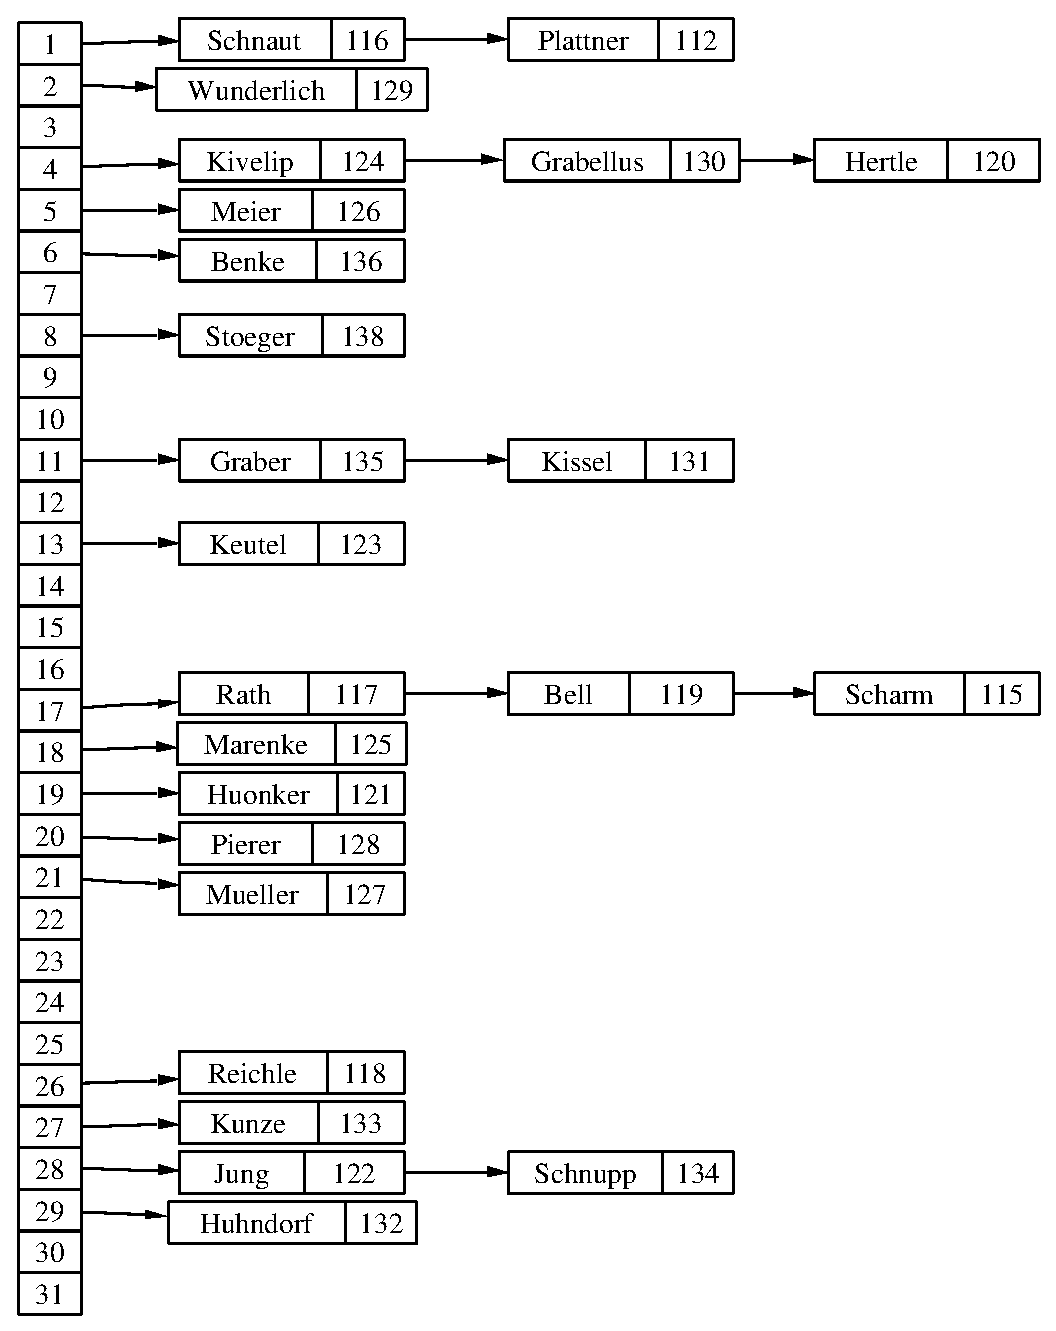
\epsfig{file=hash-table,scale=0.6}} 
  \caption{Eine Hash-Tabelle}
  \label{fig:hash-example}
\end{figure}

\noindent
Leider hat diese naive Implementierung mehrere Probleme: 
\begin{enumerate}
\item Das Feld, das wir anlegen m�ssen, hat eine Gr��e von \\[0.2cm]
      \hspace*{1.3cm} $27^8 = 282\,429\,536\,481$ \\[0.2cm]
      Eintr�gen.  Selbst wenn jeder Eintrag nur die Gr��e zweier Maschinen-Worte hat und
      ein Maschinen-Wort aus 4 Byte besteht, so br�uchten wir 
      etwas mehr als ein Terabyte um eine
      solche Tabelle anzulegen.
\item Falls zwei Namen sich erst nach dem 8-ten Buchstaben unterscheiden, k�nnen 
      wir zwischen diesen Namen nicht mehr unterscheiden. 
\end{enumerate}
Wir k�nnen diese Probleme wir folgt l�sen:
\begin{enumerate}
\item Wir �ndern die Funktion \texttt{code} so ab, dass das Ergebnis
      immer kleiner-gleich einer vorgegebene Zahl \texttt{size} ist.  Die Zahl
      \texttt{size} gibt dabei die Gr��e eines Feldes an und ist so klein,
      dass wir ein solches Feld bequem anlegen k�nnen.

      Eine einfache M�glichkeit, die Funktion \textsl{code} entsprechend abzu�ndern,
      besteht in folgender Implementierung: \\[0.2cm]
      \hspace*{1.3cm} 
      $\textsl{code}(c_0c_1\cdots c_n) = \left(\sum\limits_{i=0}^n \textsl{ord}(c_i) \cdot
        27^i\right) \;\%\; \texttt{size} + 1$.
      \\[0.2cm]
      Um einen �berlauf zu vermeiden, k�nnen wir f�r $k=n,n-1,\cdots,1,0$ die Teilsummen $s_k$
      wie folgt induktiv definieren:
      \begin{enumerate}
      \item $s_n = \textsl{ord}(c_n)$
      \item $s_{k} = \left(\textsl{ord}(c_{k}) + s_{k+1} \cdot 27 \right) \;\%\; \texttt{size}$
      \end{enumerate}
      Dann gilt
      \hspace*{1.3cm} 
      $s_0 + 1 = \left(\sum\limits_{i=0}^n \textsl{ord}(c_i) \cdot 27^i\right) \;\%\; \texttt{size} + 1$.
\item In dem Feld der Gr��e \texttt{size} speichern wir nun nicht mehr die Werte, sondern statt dessen
      Listen von Paaren aus Schl�sseln und Werten.  Dies ist notwendig, denn wir k�nnen
      nicht verhindern, dass die Funktion \texttt{code}() f�r zwei verschiedene
      Schl�ssel den selben Index liefert.
\end{enumerate}
Abbildung \ref{fig:hash-example} auf Seite \pageref{fig:hash-example} zeigt, wie ein Feld,
in dem Listen von Paaren abgebildet sind, aussehen kann.  Ein solches Feld bezeichnen wir
als Hash-Tabelle.  Wir diskutieren nun die Implementierung dieser Idee in \textsc{Setlx}.



\begin{figure}[!ht]
  \centering
\begin{Verbatim}[ frame         = lines, 
                  framesep      = 0.3cm, 
                  labelposition = bottomline,
                  numbers       = left,
                  numbersep     = -0.2cm,
                  xleftmargin   = 0.0cm,
                  xrightmargin  = 0.0cm
                ]
    class hashTable(n) {
        mSize    := n;
        mEntries := 0;  // number of entries
        mArray   := [ {} : i in [1 .. mSize] ];
        mAlpha   := 2;  // load factor
    
        static {
            sOrd    := { [ char(i), i ] : i in [ 0 .. 127 ] };
            sPrimes := [ 3, 7, 13, 31, 61, 127, 251, 509, 1021, 2039, 
                         4093, 8191, 16381, 32749, 65521, 131071, 
                         262139, 524287, 1048573, 2097143, 4194301, 
                         8388593, 16777213, 33554393, 67108859, 
                         134217689, 268435399, 536870909, 1073741789, 
                         2147483647 
                       ];    
            hashCode := procedure(s)          { ... };
            find     := procedure(key)        { ... };
            insert   := procedure(key, value) { ... };
            rehash   := procedure()           { ... };
            delete   := procedure(key)        { ... };    
        }
    }
\end{Verbatim}
\vspace*{-0.3cm}
  \caption{Outline of the class \texttt{hashTable}.}
  \label{fig:hashTable.stlx-outline}
\end{figure}

Figure \ref{fig:hashTable.stlx-outline} shows the outline of the class \texttt{hashTable}.  
\begin{enumerate}
\item The constructor is called with one argument.  This argument $n$ is the initial size
      of the array storing the different key-value lists.  The constructor constructs an empty hash
      table with the given capacity.
\item \texttt{mSize} is the actual size of the array that stores the different key-value lists.
      Although this variable is initialized as $n$, it can later be increased.  This happens
      if the hash table becomes overcrowded.
\item \texttt{mEntries} is the number key-value pairs that are stored in this hash map.
      Since, initially, this map is entry, \texttt{mEntries} is  initialized as $0$.
\item \texttt{mArray} is the array containing the list of key value pairs.

      In our implementation, the key-value pairs are not stored in a list but, instead, they are
      stored in a set.  Since every key occurs at most once, this set can be interpreted as a
      functional relation.  Therefore, looking up a key is more efficient than it would be if we had
      used a list.  Although we actually use a relation instead of a list, we will still call
      the relation the \emph{list of key-value pairs}.

      As the hash map is initially empty, all entries of \texttt{mArray} are initialized as empty sets.
\item \texttt{mAlpha} is the \emph{load factor} of our hash table.  If at any point in time, we have
      \\[0.2cm]
      \hspace*{1.3cm}
      $\texttt{mEntries} > \texttt{mAlpha} \cdot \texttt{mSize}$,
      \\[0.2cm]
      then we consider our hash table to be \emph{overcrowded}.  In that case, we would increase the size
      of the array \texttt{mArray}.  To determine the best value for \texttt{mAlpha}, we have to
      make a tradeoff:  If \texttt{mAlpha} is too big, many entries in the array \texttt{mArray}
      would be empty and thus we would waste space.  On the other hand, if \texttt{mAlpha} is too
      small, the key-value lists would become very long and hence it would take too much time to
      search for a given key in one of these lists.
\item Our implementation maintains two static variables.
  \begin{enumerate}
  \item \texttt{sOrd} is a functional relation mapping characters to \textsc{Ascii} codes.
        This relation is needed for the efficient computation of the method \texttt{hashCode}
        discussed below.

        In \texttt{SetlX} there is no function that returns the \textsc{Ascii} code of a given character.
        Fortunately, it is easy to implement this function as a binary relation via the function
        $\mathtt{char}(i)$.  Given a number $i \in \{0,\cdots,127\}$, the function $\mathtt{char}(i)$
        returns the character that has \textsc{Ascii} code $i$.  The relation \texttt{sOrd} is the inverse
        of the function \texttt{char}.
  \item \texttt{sPrimes} is a list of prime numbers.  Roughly, these prime numbers double in size.
        The reason is that performance of a hash table is best if the size of \texttt{mArray} is a
        prime number.  When \texttt{mArray} get overcrowded, the idea is to, more or less, double
        the size of \texttt{mArray}.  To achieve this, the variable \texttt{sPrimes} is needed.
  \end{enumerate}
\end{enumerate}
Next, we discuss the implementation of the various methods.

\begin{figure}[!ht]
\centering
\begin{Verbatim}[ frame         = lines, 
                  framesep      = 0.3cm, 
                  firstnumber   = 1,
                  labelposition = bottomline,
                  numbers       = left,
                  numbersep     = -0.2cm,
                  xleftmargin   = 0.0cm,
                  xrightmargin  = 0.0cm,
                ]
        hashCode := procedure(s) {
            return hashCodeAux(s) + 1;
        };
        hashCodeAux := procedure(s) {
            if (s == "") {
                return 0;
            }
            return (sOrd[s[1]] + 128 * hashCodeAux(s[2..])) % mSize;
        };
\end{Verbatim}
\vspace*{-0.3cm}
\caption{Implementation of the method \texttt{hashCode}.}
\label{fig:hashTable.stlx-hashCode}
\end{figure}

Figure gives the implementation of the method \texttt{hashCode}.
\begin{enumerate}
\item The function $\texttt{hashCode}(s)$ takes a string $s$ and computes a hash code for this string.
      This hash code satisfies
      \\[0.2cm]
      \hspace*{1.3cm}
      $\mathtt{hashCode}(s) \in \{ 1, \cdots, \mathtt{mSize} \}$.
      \\[0.2cm]
      Therefore, the hash code can be used to index into \texttt{mArray}.  The implementation of
      \texttt{hashCode} works by calling $\texttt{hashCodeAux}(s)$.  As the values returned by
      $\texttt{hashCodeAux}(s)$ are elements of the set
      \\[0.2cm]
      \hspace*{1.3cm}
      $\mathtt{hashCode}(s,n) \in \{ 0, \cdots, \mathtt{mSize}-1 \}$      
      \\[0.2cm]
      we have to add $1$ so that the hash code is an element of 
      \\[0.2cm]
      \hspace*{1.3cm}
      $\mathtt{hashCode}(s,n) \in \{ 1, \cdots, \mathtt{mSize} \}$.      
\item The function $\mathtt{hashCodeAux}(s)$ is defined by induction on the string $s$.
      If the string $s$ has length $m$ we have
      \\[0.2cm]
      \hspace*{1.3cm}
      $\mathtt{hashCodeAux}(s,n) := \left(\sum\limits_{i=1}^m \mathtt{ord}(s[i]) \cdot 128^{i-1}\right) \;\mathtt{\%}\; \mathtt{mSize}$.
      \\[0.2cm]
      Here, given an \textsc{Ascii} character $c$, the expression  $\mathtt{ord}(c)$ computes the
      \textsc{Ascii} code of  $c$.
\end{enumerate}

\begin{figure}[!ht]
\centering
\begin{Verbatim}[ frame         = lines, 
                  framesep      = 0.3cm, 
                  firstnumber   = 1,
                  labelposition = bottomline,
                  numbers       = left,
                  numbersep     = -0.2cm,
                  xleftmargin   = 0.8cm,
                  xrightmargin  = 0.8cm,
                ]
        find := procedure(key) {
             index := hashCode(key);
             aList := mArray[index];
             return aList[key];
        };
\end{Verbatim}
\vspace*{-0.3cm}
\caption{Implementation of \texttt{find}.}
\label{fig:hashTable.stlx-find}
\end{figure}

Figure \ref{fig:hashTable.stlx-find} show the implementation of the method \texttt{find}.
\begin{enumerate}
\item First, we compute the index of the key-value list that is used to store the given
      \texttt{key}.
\item Next, we retrieve this key-value list from the array \texttt{mArray}.
\item Finally, we look up the information stored under the given \texttt{key} in this 
      key-value list.  Remember, that the key-value list is not an actual list but rather a binary
      relation.  We can use the notation \texttt{aList[key]} to retrieve the value associated with
      the given key.
\end{enumerate}

\begin{figure}[!ht]
\centering
\begin{Verbatim}[ frame         = lines, 
                  framesep      = 0.3cm, 
                  firstnumber   = 1,
                  labelposition = bottomline,
                  numbers       = left,
                  numbersep     = -0.2cm,
                  xleftmargin   = 0.8cm,
                  xrightmargin  = 0.8cm,
                ]
        insert := procedure(key, value) {
             if (mEntries > mSize * mAlpha) {
                 rehash();
                 insert(key, value);
                 return;
             }
             index      := hashCode(key);
             aList      := mArray[index];
             oldSz      := #aList;
             aList[key] := value;
             newSz      := #aList;
             this.mArray[index] := aList;
             if (newSz > oldSz) {
                 this.mEntries += 1;
             }    
        };
\end{Verbatim}
\vspace*{-0.3cm}
\caption{Implementation of the method \texttt{insert}.}
\label{fig:hashTable.stlx-insert}
\end{figure}

Figure \ref{fig:hashTable.stlx-insert} shows the implementation of the method \texttt{insert}.
The implementation works as follows.
\begin{enumerate}
\item First, we check whether our has table is already overcrowded.
      In this case, we \emph{rehash}, which means we roughly double the size of \texttt{mArray}.
      How the method \texttt{rehash} works in detail is explained later.
      After rehashing, the \texttt{key} is inserted via a recursive call.
\item If we don't have to rehash, we compute the index of the key-value list that has to store
      \texttt{mKey}, retrieve the associated key-value list, and finally associate the
      \texttt{value} with the given key.  When inserting the given key-value
      pair into the key-value list there can be two cases.
      \begin{enumerate}
      \item The key-value list already stores information for the given \texttt{key}.
            In this case, the number of entries of the hash table is not changed.
      \item If the given \texttt{key} is not yet present in the given key-value list,
            the number of entries needs to be incremented.
      \end{enumerate}
      In order to distinguish these two cases, we compare the size of the key-value list before
      the insertion with the size after the insertion.     
\end{enumerate}


\begin{figure}[!ht]
\centering
\begin{Verbatim}[ frame         = lines, 
                  framesep      = 0.3cm, 
                  firstnumber   = 1,
                  labelposition = bottomline,
                  numbers       = left,
                  numbersep     = -0.2cm,
                  xleftmargin   = 0.0cm,
                  xrightmargin  = 0.0cm,
                ]
        rehash := procedure() {
             prime  := min({ p in sPrimes | p * mAlpha > mEntries });
             bigMap := hashTable(prime);
             for (aList in mArray) {
                 for ([k, v] in aList) {
                     bigMap.insert(k, v);
                 }    
             }
             this.mSize  := prime;
             this.mArray := bigMap.mArray;
        };
\end{Verbatim}
\vspace*{-0.3cm}
\caption{Implementation of the method \texttt{rehash}.}
\label{fig:hashTable.stlx-rehash}
\end{figure}


Figure \ref{fig:hashTable.stlx-rehash} show the implementation of the method
$\mathtt{rehash}()$.  This method is called if the hash table becomes overcrowded.  The idea is to
roughly double the size of \texttt{mArray}.  Theoretical considerations that are  beyond the scope
of this lecture show that it is beneficial if the size of \texttt{mArray} is a prime number.
Hence, we look for the first prime number \texttt{prime} such that \texttt{prime} times the load
factor \texttt{mAlpha} is bigger than the
number of entries since this will assure that, on average, the number of entries in each key-value
list is less than the load factor \texttt{mAlpha}.  After we have determined \texttt{prime}, we
proceed as follows: 
\begin{enumerate}
\item We create a new empty hash table of size \texttt{prime}.
\item Next, we move the key-value pairs from the given has table to the new hash table.
\item Finally, the array stored in the new hash table is moved to the given hash table
      and the size is adjusted correspondingly.
\end{enumerate}





\begin{figure}[!ht]
\centering
\begin{Verbatim}[ frame         = lines, 
                  framesep      = 0.3cm, 
                  firstnumber   = last,
                  labelposition = bottomline,
                  numbers       = left,
                  numbersep     = -0.2cm,
                  xleftmargin   = 0.8cm,
                  xrightmargin  = 0.8cm,
                ]
        delete := procedure(key) {
             index      := hashCode(key);
             aList      := mArray[index];
             oldSz      := #aList;
             aList[key] := om;
             newSz      := #aList;
             this.mArray[index] := aList;
             if (newSz < oldSz) {
                 this.mEntries -= 1;
             }    
        };
\end{Verbatim}
\vspace*{-0.3cm}
\caption{Die Funktion $\mathtt{delete}(\textsl{map}, \textsl{key})$.}
\label{fig:hashTable.stlx-delete}
\end{figure}

Finally, we discuss the implementation of the method \texttt{delete} that is shown in Figure
\ref{fig:hashTable.stlx-delete}.  The implementation of this method is similar to the implementation
of the method \texttt{insert}.   The implementation makes use of the fact that in order to delete
a key-value pair from a function relation in \textsc{SetlX} it is possible to assign the value
\texttt{om} to the \texttt{key} that needs to be deleted. Note, that we have to be careful to
maintain the number of entries since we do not know whether the list of key-value pairs has an entry
for the given \texttt{key}.

However, there is one crucial difference compared to the implementation of \texttt{insert}.
We do not rehash the hash table if the number of entries falls under certain thresh hold.
Although this could be done and there are implementations of hash tables that readjust the size of the
hash table if the hash table gets underpopulated, we don't do so here because often a table will
grow again after it has shrunk and in that case rehashing would be counter productive.


Falls wir in unserer Implementierung tats�chlich mit Listen und nicht mit Mengen arbeiten w�rden, dann
k�nnte die Komplexit�t der Methoden \textsl{find}, \textsl{insert} und \textsl{delete}
im ung�nstigsten Fall linear mit der Anzahl der Eintr�ge in der Hash-Tabelle wachsen.  Dieser
Fall tritt dann auf, wenn die Funktion $\texttt{hashTable}(k,n)$ f�r alle Schl�ssel $k$ den
selben Wert berechnet.  Dieser Fall ist allerdings sehr unwahrscheinlich.  Der Normalfall
ist der, dass alle Listen etwa gleich lang sind.  Die durchschnittliche L�nge  einer Liste
ist dann \\[0.2cm]
\hspace*{1.3cm} $\alpha = \displaystyle \frac{\mathtt{count}}{\mathtt{size}}$. \\[0.2cm]
Hierbei ist $\mathtt{count}$ die Gesamtzahl der Eintr�ge in der Tabelle und \texttt{size}
gibt die Gr��e der Tabelle an.  Das Verh�ltnis $\alpha$ dieser beiden Zahlen ist genau der
 \emph{Auslastungs-Faktor} der Hash-Tabelle.  In der Praxis zeigt sich, dass
$\alpha$ kleiner als 4 sein sollte.  In \textsl{Java} gibt es die Klasse \textsl{HashMap},
die Abbildungen als Hash-Tabellen implementiert.  Dort hat der per Default eingestellte maximale
Auslastungs-Faktor sogar nur den Wert \texttt{0.75}.


\subsection{Further Reading}
In this section, we have discussed hash tables only briefly.  The reason is that, although hash tables are very
important in practice, a thorough treatment requires quite a lot of mathematics, see for example the
third volume of Donald Knuth's ``The Art of Computer Programming'' \cite{knuth:1998b}.  For this
reason, the design of a hash function is best left for experts.  In practice, hash tables are
quite a bit faster than \textsl{AVL}-trees or \emph{red-black} trees.  However, this is only true if
the hash function that is used is able to spread the keys uniformly.  If this assumption is
violated, the use of a hash table can lead to serious performance 
bugs.  If, instead, a good
implementation of red-black-trees is used, the program might be slower in general but are certain to
be protected from the ugly surprises that can result from a poor hash function.  My advice for the reader
therefore is to use hashing only if the performance is really critical and you are sure that your
hash function is distributing the keys nicely.


\section{Applications}
Both \texttt{C++} and \textsl{Java} provide maps.  In \texttt{C++}, maps are part of the standard
template library, while \textsl{Java} offers the interface \texttt{Map} that is implemented both by
the class \texttt{TreeMap} and the class \texttt{HashMap}. Furthermore, all modern script languages provide maps.
For example, in \textsl{Perl} \cite{Wall92}, maps are known as \emph{associative arrays}, in \textsl{Lua} 
\cite{ierusalimschy:2006,Ieru96a} maps are called tables, and in \textsl{Python} 
\cite{vanRossum:95,lutz:09} map are called \emph{dictionaries}.  

Later, when we discuss Dijkstra's algorithm for finding the shortest path in a graph we will see an
application of maps.

%%% Local Variables: 
%%% mode: latex
%%% TeX-master: "algorithms"
%%% End: 

\chapter{Priority Queues \label{chap:prioqueue}}
Um den Begriff der  \emph{Priorit�ts-Warteschlange} zu verstehen, betrachten wir zun�chst
den Begriff der \emph{Warteschlange}.  Dort werden Daten hinten eingef�gt und vorne werden
Daten entnommen. Das f�hrt dazu, dass Daten in der selben Reihenfolge entnommen werden,
wie sie eingef�gt werden.  Anschaulich ist das so wie bei der Warteschlange vor einer
Kino-Kasse, wo die Leute in der Reihenfolge bedient werden, in der sie sich anstellen.
Bei einer Priorit�ts-Warteschlange haben die Daten zus�tzlich Priorit�ten.  Es wird immer
das Datum entnommen, was die h�chste Priorit�t hat.  Anschaulich ist das so wie im
Wartezimmer eines Zahnarztes. Wenn Sie schon eine Stunde gewartet haben und dann ein
Privat-Patient aufkreuzt, dann m�ssen Sie halt noch eine Stunde warten, weil der
Privat-Patient eine h�here Priorit�t hat.

Priorit�ts-Warteschlangen spielen in vielen Bereichen der Informatik  eine wichtige
Rolle.  Wir werden Priorit�ts-Warteschlangen sp�ter sowohl in dem Kapitel �ber
Daten-Kompression als auch bei der Implementierung des Algorithmus zur Bestimmung
k�rzester Wege in einem Graphen einsetzen.  Daneben werden Priorit�ts-Warteschlangen unter anderem in
Simulations-Systemen und beim Scheduling von Prozessen in Betriebs-Systemen eingesetzt.


\section[Definition]{Definition des ADT \textsl{PrioQueue}}
Wir versuchen den Begriff der Priorit�ts-Warteschlange jetzt formal durch Definition eines
abstrakten Daten-Typs zu fassen.
Wir geben hier eine eingeschr�nkte Definition von Priorit�ts-Warteschlangen, die nur die
Funktionen enth�lt, die wir sp�ter f�r den Algorithmus von Dijkstra ben�tigen.
\begin{Definition}[Priorit�ts-Warteschlange] \hspace*{\fill} \\
{\em
  Wir definieren den abstrakten Daten-Typ der \emph{Priorit�ts-Warteschlange} wie folgt:
  \begin{enumerate}
  \item Als Namen w�hlen wir \textsl{PrioQueue}.
  \item Die Menge der Typ-Parameter ist \\[0.1cm]
        \hspace*{1.3cm} $\{ \textsl{Priority}, \textsl{Value} \}$.

        Dabei mu� auf der Menge $\textsl{Priority}$ eine totale Quasi-Ordnung $<$ existieren,
        so dass wir die Priorit�ten verschiedener Elemente vergleichen k�nnen. 
  \item Die Menge der Funktions-Zeichen ist \\[0.1cm]
       \hspace*{1.3cm} 
       $\{ \textsl{prioQueue}, \textsl{insert}, \textsl{remove}, \textsl{top} \}$.
  \item Die Typ-Spezifikationen der Funktions-Zeichen sind gegeben durch:
        \begin{enumerate}
        \item $\textsl{prioQueue}: \textsl{PrioQueue}$

              Der Aufruf ``$\textsl{prioQueue}()$'' erzeugt eine leere
              Priorit�ts-Warteschlange. 
        \item $\textsl{top}: \textsl{PrioQueue}  \rightarrow (\textsl{Priority} \times \textsl{Value}) \cup \{\Omega\}$

              Der Aufruf $Q.\textsl{top}()$ liefert ein Paar $\pair(p,v)$.  Dabei ist $v$ ein Element
              aus $Q$, das eine maximale Priorit�t hat. $p$ ist die Priorit�t des Elements $v$.
        \item $\textsl{insert}: \textsl{PrioQueue} \times \textsl{Priority} \times \textsl{Value} \rightarrow \textsl{PrioQueue}$

              Der Aufruf $Q.\textsl{insert}(p,v)$ f�gt das Element $v$ mit der Priorit�t $p$ in
              die Priorit�ts-Warteschlange $Q$ ein.  
        \item $\textsl{remove}: \textsl{PrioQueue} \rightarrow \textsl{PrioQueue}$

              Der Aufruf $Q.\textsl{remove}()$ entfernt aus der Priorit�ts-Warteschlange
              $Q$ das Element, das durch den Ausdruck $Q.\texttt{top}()$ berechnet wird.
        \end{enumerate}
\item Bevor wir das Verhalten der einzelnen Methoden axiomatisch definieren, m�ssen wir
      noch festlegen, was wir unter den \emph{Priorit�ten} verstehen wollen, die den
      einzelnen Elementen aus $\textsl{Value}$ zugeordnet sind.  Wir nehmen an, dass die
      Priorit�ten Elemente einer Menge $\textsl{Priority}$ sind und dass auf der Menge \textsl{Priority}
      eine totale Quasi-Ordnung $\leq$ existiert. Falls dann $p_1 < p_2$ ist, sagen wir, 
      dass $p_1$ eine h�here Priorit�t als $p_2$ hat.  Dies erscheint im ersten Moment vielleicht
      paradox. Es wird aber sp�ter verst�ndlich, wenn wir den Algorithmus zur
      Berechnung k�rzester Wege von Dijkstra diskutieren. Dort sind die Priorit�ten
      Entfernungen im Graphen und die Priorit�t eines Knotens ist um so h�her, je n�her
      der Knoten zu einem als \emph{Startknoten} ausgezeichneten Knoten ist. 

      Wir spezifizieren das Verhalten der Methoden nun dadurch, dass wir eine einfache
      \emph{Referenz-Implementierung} des ADT \textsl{PrioQueue} angeben und dann fordern,
      dass sich eine Implementierung des ADT \textsl{PrioQueue} genauso verh�lt wie unsere
      Referenz-Implementierung.  Bei unserer Referenz-Implementierung stellen wir eine
      Priorit�ts-Warteschlange durch eine Menge von Paaren von Priorit�ten und Elementen 
      dar.   F�r solche Mengen definieren wir unserer Methoden wie folgt.
      \begin{enumerate}
      \item $\textsl{prioQueue}() = \{\}$,

             der Konstruktor erzeugt also eine leere
            Priorit�ts-Warteschlange, die als leere Menge dargestellt wird. 
      \item $Q.\textsl{insert}(p, v) = Q \cup \{ \pair(p,v) \}$,
        
            Um ein Element $v$ mit einer Priorit�t $p$ in die Priorit�ts-Warteschlange 
            $Q$ einzuf�gen, reicht es aus, das Paar $\pair(p,v)$ zu der Menge $Q$ hinzuzuf�gen.
      \item Wenn $Q$ leer ist, dann ist $Q.\textsl{top}()$ undefiniert: \\[0.1cm]
            \hspace*{1.3cm} $Q = \{\} \;\rightarrow\; Q.\textsl{top}() = \Omega$.
     \item Wenn $Q$ nicht leer ist, wenn es also ein Paar $\pair(p_1, v_1)$ in $Q$
              gibt, dann liefert $Q.\textsl{top}()$ ein Paar $\pair(p_2,v)$ aus der Menge
              $Q$, so dass die Priorit�t $p_2$ minimal wird.  Dann gilt also f�r
              alle $\pair(p_1,v_1) \in Q$, dass $p_2 \leq p_1$ ist.  Formal k�nnen wir schreiben:
              \\[0.1cm]
              \hspace*{1.3cm} 
              $\pair(p_1,v_1) \in Q \;\wedge\; Q.\textsl{top}() = \pair(p_2,v_2)
              \;\rightarrow\; p_2 \leq p_1 \;\wedge\; \pair(p_2,v_2) \in Q$.
      \item Falls $Q$ leer ist, dann �ndert $\textsl{remove}()$ nichts daran: \\[0.1cm]
            \hspace*{1.3cm} $Q = \{\} \rightarrow Q.\textsl{remove}() = Q$.
      \item Sonst entfernt $Q.\textsl{remove}()$ das Paar, dass von $Q.\textsl{top}()$ berechnet wird: \\[0.1cm]
            \hspace*{1.3cm} 
            $Q \not= \{\} \rightarrow Q.\textsl{remove}() = Q \backslash \bigl\{ Q.\textsl{top}() \bigr\}$.
      \end{enumerate}
\end{enumerate}
}
\end{Definition}

Wir k�nnen den abstrakten Daten-Typ \textsl{PrioQueue} dadurch implementieren,
dass wir eine Priorit�ts-Warteschlange durch eine Liste realisieren, in der die Elemente
aufsteigend geordnet sind. Die einzelnen Operationen werden dann wie folgt implementiert:
\begin{enumerate}
\item $\textsl{prioQueue}()$ erzeugt eine leere Liste.
\item $Q.\textsl{insert}(d)$ kann durch die Prozedur \texttt{insert} implementiert werden,
      die wir beim ``\emph{Sortieren durch Einf�gen}'' entwickelt haben.
\item $Q.\textsl{top}()$ gibt das erste Element der Liste zur�ck.
\item $Q.\textsl{remove}()$ entfernt das erste Element der Liste.
\end{enumerate}
Bei dieser Implementierung ist die Komplexit�t der Operation $\textsl{insert}()$ 
linear in der
Anzahl $n$ der Elemente der Priorit�ts-Warteschlange.  Alle anderen Operationen sind
konstant. Wir werden jetzt eine andere
Implementierung vorstellen, bei der die Komplexit�t von $\textsl{insert}()$ 
 den Wert $\Oh\bigl(\log(n)\bigr)$ hat.  Dazu f�hren wir die Daten-Struktur eines
 \emph{Heaps} ein.

\section[Heaps]{Die Daten-Struktur \emph{Heap}}
Wir definieren die Menge \textsl{Heap}\footnote{
Der Begriff \textsl{Heap} wird in der Informatik f�r zwei v�llig unterschiedliche Dinge
verwendet:  Zum einen wird die in diesem Abschnitt beschriebene Daten-Struktur als
\textsl{Heap} bezeichnet, zum anderen wird der Teil des Speichers, in dem dynamisch
erzeugte Objekte abgelegt werden, ebenfalls als \textsl{Heap} bezeichnet.}
induktiv als Teilmenge der Menge $\Bin$ der
bin�ren B�ume. Dazu definieren wir zun�chst f�r eine Priorit�t $p_1\in \textsl{Priority}$ und
einen bin�ren Baum $b \in \Bin$ die Relation $p_1 \leq b$ durch Induktion �ber $b$.
Die Intention ist dabei, dass $p_1 \leq b$ genau dann gilt, wenn f�r jede Priorit�t $p_2$,
die in $b$ auftritt,  $p_1 \leq p_2$ gilt. Die formale Definition ist wie folgt:
\begin{enumerate}
\item $p_1 \leq \textsl{Nil}$,

      denn in dem leeren Baum treten �berhaupt keine Priorit�ten auf.
\item $p_1 \leq \textsl{Node}(p_2,v,l,r) \;\stackrel{\mbox{\scriptsize def}}{\longleftrightarrow}\; p_1 \leq p_2 \;\wedge\; p_1 \leq l \;\wedge\; p_1 \leq r$,
         
      denn $p_1$ ist genau dann kleiner-gleich als alle Priorit�ten, die in dem Baum 
      $\textsl{Node}(p_2,v,l,r)$ auftreten, wenn $p_1 \leq p_2$ gilt und wenn zus�tzlich
      $p_1$ kleiner-gleich als alle Priorit�ten ist, die in $l$ oder $r$ auftreten.
\end{enumerate}
Als n�chstes definieren wir eine Funktion \\[0.1cm]
\hspace*{1.3cm} $\textsl{count}: \Bin \rightarrow \mathbb{N}$, \\[0.1cm]
die f�r einen bin�ren Baum die Anzahl der Knoten berechnet.  Die Definition erfolgt durch
Induktion:
\begin{enumerate}
\item $\textsl{Nil}.\textsl{count}() = 0$.
\item $\textsl{Node}(p,v,l,r).\textsl{count}() = 1 + l.\textsl{count}() + r.\textsl{count}()$.
\end{enumerate}
Mit diesen Vorbereitungen k�nnen wir nun die Menge \textsl{Heap} induktiv definieren:
\begin{enumerate}
\item $\textsl{Nil} \in \textsl{Heap}$.
\item $\textsl{Node}(p,v,l,r) \in \textsl{Heap}$ g.d.w. folgendes gilt:
      \begin{enumerate}
      \item $p \leq l \;\wedge\; p \leq r$,

            Die Priorit�t an der Wurzel ist also kleiner-gleich als alle anderen Priorit�ten.
            Diese Bedingung bezeichnen wir auch als die \emph{Heap-Bedingung}.
      \item $\mid l.\textsl{count}() - r.\textsl{count}() \mid \;\leq\, 1$,

            Die Zahl der Elemente im linken Teilbaum ist also h�chstens 1 gr��er oder
            kleiner als die Zahl der Elemente im rechten Teilbaum.
            Diese Bedingung bezeichen wir als die \emph{Balancierungs-Bedingung}.  Sie ist
            ganz �hnlich zu der Balancierungs-Bedingung bei AVL-B�umen, nur dass es dort
            die H�he der B�ume ist, die verglichen wird, w�hrend wir hier die Zahl der
            im Baum gespeicherten Elemente vergleichen.
      \item $l \in \textsl{Heap} \;\wedge\; r \in \textsl{Heap}$.
      \end{enumerate}
\end{enumerate}
Aus der \emph{Heap-Bedingung} folgt, dass ein nicht-leerer Heap die Eigenschaft hat, dass
das Element, welches an der Wurzel steht, immer die h�chste Priorit�t hat.  Abbildung
\ref{fig:heap-list} auf Seite \pageref{fig:heap-list} zeigt einen einfachen Heap.
In den Knoten steht im oberen Teil die Priorit�ten (in der Abbildung sind das nat�rliche Zahlen) und
darunter stehen die Elemente (in der Abbildung sind dies Buchstaben).

\begin{figure}[!t]
  \centering
  \framebox{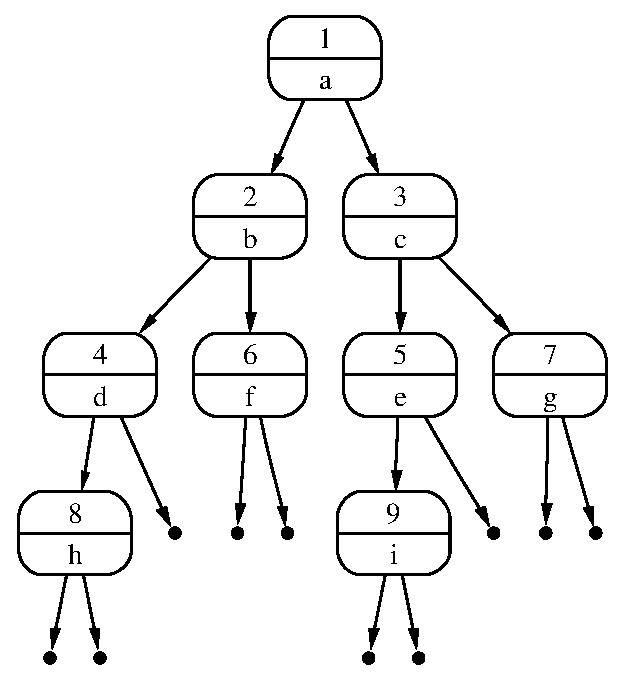
\epsfig{file=heap-with-holes,scale=0.7}} 
  \caption{Ein Heap}
  \label{fig:heap-list}
\end{figure}


Da Heaps bin�re
B�ume sind, k�nnen wir Sie ganz �hnlich wie geordnete bin�re B�ume  implementieren. 
Wir stellen zun�chst Gleichungen auf, die die Implementierung der verschiedenen Methoden
beschreiben.  Wir beginnen mit der  Methode \textsl{top}.  Es gilt:
\begin{enumerate}
\item $\textsl{Nil}.\textsl{top}() = \Omega$.
\item $\textsl{Node}(p,v,l,r).\textsl{top}() = \pair(p,v)$,

      denn aufgrund der Heap-Bedingung wird das Element mit der h�chsten Priorit�t 
      an der Wurzel gespeichert.
\end{enumerate}
Die Methoden \textsl{insert} m�ssen wir nun so implementieren, dass
sowohl die Balancierungs-Bedingung als auch die Heap-Bedingung erhalten bleiben.
\begin{enumerate}
\item $\textsl{Nil}.\textsl{insert}(p,v) = \textsl{Node}(p,v,\textsl{Nil}, \textsl{Nil})$.
\item $p_{\mathrm{top}} \leq p \;\wedge\; l.\textsl{count}() \leq r.\textsl{count}() \;\rightarrow $   \\[0.1cm]
      \hspace*{1.3cm} 
      $\textsl{Node}(p_{\mathrm{top}},v_\mathrm{top},l,r).\textsl{insert}(p,v) =
                 \textsl{Node}\bigl(p_\mathrm{top},v_\mathrm{top},l.\textsl{insert}(p,v), r\bigr)$.

      Falls das einzuf�gende Paar eine geringere oder die selbe Priorit�t hat wie das
      Paar, welches sich an der Wurzel befindet, und falls zus�tzlich die Zahl der Paare im linken Teilbaum
      kleiner-gleich der Zahl der Paare im rechten Teilbaum ist, dann f�gen wir das
      Paar im linken Teilbaum ein.
\item $p_{\mathrm{top}} \leq p \;\wedge\; l.\textsl{count}() > r.\textsl{count}() \;\rightarrow $   \\[0.1cm]
      \hspace*{1.3cm} 
      $\textsl{Node}(p_{\mathrm{top}},v_\mathrm{top},l,r).\textsl{insert}(p,v) =
                 \textsl{Node}\bigl(p_\mathrm{top},v_\mathrm{top},l,r.\textsl{insert}(p,v)\bigr)$.

      Falls das einzuf�gende Paar eine geringere oder die selbe Priorit�t hat als das
      Paar an der Wurzel und falls zus�tzlich die Zahl der Paare im linken Teilbaum
      gr��er als die Zahl der Paare im rechten Teilbaum ist, dann f�gen wir das
      Paar im rechten Teilbaum ein.
\item $p_{\mathrm{top}} > p \;\wedge\; l.\textsl{count}() \leq r.\textsl{count}() \;\rightarrow $ \\[0.1cm]
      \hspace*{1.3cm} 
      $\textsl{Node}(p_{\mathrm{top}},v_\mathrm{top},l,r).\textsl{insert}(p,v) =
                 \textsl{Node}\bigl(p,v,l.\textsl{insert}(p_\mathrm{top},v_\mathrm{top}), r\bigr)$.

      Falls das einzuf�gende Paar eine h�here Priorit�t hat als das Paar an
      der Wurzel, dann m�ssen wir das neu einzuf�gende Paar an der Wurzel
      positionieren.  Das Paar, das dort vorher steht, f�gen wir in den linken
      Teilbaum ein, falls  die Zahl der Paare im linken Teilbaum
      kleiner-gleich der Zahl der Paare im rechten Teilbaum ist.
\item $p_{\mathrm{top}} > p \;\wedge\; l.\textsl{count}() > r.\textsl{count}() \;\rightarrow $ \\[0.1cm] 
      \hspace*{1.3cm} 
      $\textsl{Node}(p_{\mathrm{top}},v_\mathrm{top},l,r).\textsl{insert}(p,v) =
                 \textsl{Node}\bigl(p,v,l,r.\textsl{insert}(p_\mathrm{top},v_\mathrm{top})\bigr)$.

      Falls wir das einzuf�gende Paar an der Wurzel
      positionieren m�ssen und die Zahl der Paare im linken Teilbaum
      gr��er als die Zahl der Paare im rechten Teilbaum ist,
      dann m�ssen wir das Paar, das vorher an der Wurzel stand, im rechten Teilbaum
      einf�gen.
\end{enumerate}
Als n�chstes beschreiben wir die Implementierung der Methode \textsl{remove}.
\begin{enumerate}
\item $\textsl{Nil}.\textsl{remove}() = \textsl{Nil}$,

      denn aus dem leeren Heap ist nichts mehr zu entfernen.
\item $\textsl{Node}(p,v,\textsl{Nil},r).\textsl{remove}() = r$,
  
\item $\textsl{Node}(p,v,l,\textsl{Nil}).\textsl{remove}() = l$,

      denn wir entfernen immer das Paar mit der h�chsten Priorit�t und das ist an der
      Wurzel.  Wenn einer der beiden Teilb�ume leer ist, k�nnen wir einfach den anderen
      zur�ck geben.

      Jetzt betrachten wir die F�lle, wo keiner der beiden Teilb�ume leer ist.
      Dann muss entweder das Paar an der Wurzel des linken Teilbaums
      oder das Paar an der Wurzel des rechten Teilbaums an die Wurzel aufr�cken.
      Welches dieser beiden Paare wir nehmen, h�ngt davon ab, welches der Paare die h�here
      Priorit�t hat.
\item $p_1 \leq p_2 \;\wedge\; l = \textsl{Node}(p_1,v_1,l_1,r_1) \;\wedge\; r =
      \textsl{Node}(p_2,v_2,l_2,r_2) \;\rightarrow$ \\[0.1cm] 
      \hspace*{1.3cm} 
      $\textsl{Node}(p,v,l,r).\textsl{remove}() =      \textsl{Node}(p_1,v_1,l.\textsl{remove}(),r)$,

      denn wenn das Paar an der Wurzel des linken Teilbaums eine h�here Priorit�t hat
      als das Paar an der Wurzel des rechten Teilbaums, dann r�ckt dieses Paar an
      die Wurzel auf und muss folglich aus dem linken Teilbaum gel�scht werden.
\item $p_1 > p_2 \;\wedge\; l = \textsl{Node}(p_1,v_1,l_1,r_1) \;\wedge\; r = \textsl{Node}(p_2,v_2,l_2,r_2) \rightarrow$ \\[0.1cm]
      \hspace*{1.3cm} 
      $\textsl{Node}(p,v,l,r).\textsl{remove}() = \textsl{Node}(p_2,v_2,l,r.\textsl{remove}())$,

      denn wenn das Paar an der Wurzel des rechten Teilbaums eine h�here Priorit�t hat
      als das Paar an der Wurzel des linken Teilbaums, dann r�ckt dieses Paar an
      die Wurzel auf und muss folglich aus dem rechten Teilbaum gel�scht werden.  
\end{enumerate}
An dieser Stelle wird der aufmerksame Leser bemerken, dass die obige
Implementierung der Methode $\textsl{remove}()$ die Balancierungs-Bedingung verletzt.
Es ist nicht schwierig, die Implementierung so abzu�ndern, dass die
Balancierungs-Bedingung erhalten bleibt. Es zeigt sich jedoch, dass die
Balancierungs-Bedingung  nur beim Aufbau eines Heaps mittels \textsl{insert}() wichtig ist,
denn dort garantiert sie, dass die H�he des Baums in logarithmischer Weise von der Zahl
seiner Knoten abh�ngt.  Beim L�schen wird die H�he des Baums sowieso nur kleiner, also
brauchen wir uns da keine Sorgen machen.

\exercise
Change the equations for the method \texttt{remove} so that the resulting heap satisfies the
balancing condition.



\section[Implementation]{Implementing \textsl{Heaps} in \textsc{SetlX}}

\begin{figure}[bt]
\centering
\begin{Verbatim}[ frame         = lines, 
                  framesep      = 0.3cm, 
                  firstnumber   = 1,
                  labelposition = bottomline,
                  numbers       = left,
                  numbersep     = -0.2cm,
                  xleftmargin   = 0.0cm,
                  xrightmargin  = 0.0cm,
                ]
    class heap() {
        mPriority := om;
        mValue    := om;
        mLeft     := om;
        mRight    := om;
        mCount    := 0;
    
      static {
          top     := procedure()     { return [mPriority, mValue]; };
          insert  := procedure(p, v) { ... };
          remove  := procedure()     { ... };
          update  := procedure(t)    { ... };
          isEmpty := [] |-> mCount == 0;
      }
    }
\end{Verbatim}
\vspace*{-0.3cm}
\caption{Outline of the class \texttt{heap}.}
\label{fig:heap.stlx-outline}
\end{figure}

\noindent
Next, we present an implementation of heaps in \textsc{SetlX}. 
Figure \ref{fig:heap.stlx-outline} shows an outline of the class \texttt{heap}.  An object of class
heap represents a node in a heap data structure. In order to do this, it maintains the following
member variables:
\begin{enumerate}
\item \texttt{mPriority} is the priority of the value stored at this node,
\item \texttt{mValue}    stores the corresponding value,
\item \texttt{mLeft} and \texttt{mRight} represent the left and right subtree, respectively, while
\item \texttt{mCount}    gives the number of nodes in the subtree rooted at this node.
\end{enumerate}
The constructor initializes these member variables in a way that the resulting object represents an
empty heap.  Since a heap stores the value with the highest priority at the root, implementing the
method \texttt{top} is trivial: We just have to return the value stored at the root.
The implementation of \texttt{isEmpty} is easy, too: We just have to check whether the number of
values stored into this heap is zero.
\begin{figure}[!ht]
\centering
\begin{Verbatim}[ frame         = lines, 
                  framesep      = 0.3cm, 
                  firstnumber   = 1,
                  labelposition = bottomline,
                  numbers       = left,
                  numbersep     = -0.2cm,
                  xleftmargin   = 0.8cm,
                  xrightmargin  = 0.8cm,
                ]
    insert := procedure(priority, value) {
        if (isEmpty()) {
            this.mPriority := priority;
            this.mValue    := value;
            this.mLeft     := heap(this);
            this.mRight    := heap(this);
            this.mCount    := 1;
            return;
        }
        this.mCount += 1;
        if (priority < mPriority) {                         
            if (mLeft.mCount > mRight.mCount) {
                mRight.insert(mPriority, mValue);
            } else {
                mLeft.insert(mPriority, mValue);
            }
            this.mPriority := priority;
            this.mValue    := value;
        } else {
            if (mLeft.mCount > mRight.mCount) { 
                mRight.insert(priority, value);
            } else {
                mLeft.insert(priority, value);
            }
        }
    };
\end{Verbatim}
\vspace*{-0.3cm}
\caption{Implementation of the method \texttt{insert}.}
\label{fig:heap.stlx-insert}
\end{figure}

\noindent
Figure \ref{fig:heap.stlx-insert} show the implementation of the method \texttt{insert}.
Basically, there are two cases.
\begin{enumerate}
\item If the given heap is empty, then we store the value to be inserted at the current node.
      We have to make sure to set \texttt{mLeft} and \texttt{mRight} to empty heaps.  The reason is
      that, for every non-empty node, we want \texttt{mLeft} and \texttt{mRight} to store objects.
      Then, we can be sure that an expression like \texttt{mLeft.isEmpty()} is always well defined.
      If, however, we would allow \texttt{mLeft} to have the value \texttt{om}, then the evaluation
      of \texttt{mLeft.isEmpty()} would result in an error.
\item If the given heap is non-empty, we need another case distinction.
  \begin{enumerate}
  \item If the \texttt{priority} of the \texttt{value} to be inserted is higher\footnote{
        Remember that we have defined a priority $p_1$ to be \emph{higher} than a priority $p_2$
        iff $p_1 < p_2$.  I know that this sounds counter intuitive but unfortunately that is the
        way priorities are interpreted.  You will understand the reason for this convention later on
        when we discuss Dijkstra's \emph{shortest path algorithm}.}
        than
        \texttt{mPriority}, which is the priority of the value at the current node, then we have to 
        put \texttt{value} at the current node, overwriting \texttt{mValue}.  However, as we do not want
        to loose the value \texttt{mValue} that is currently stored at this node, we have to insert 
        \texttt{mValue} into either the left or the right subtree.  In order to keep the heap
        balanced we insert \texttt{mValue} into the smaller subtree and choose the left subtree if
        both subtrees have the same size.
  \item If the \texttt{value} to be inserted has a lower \texttt{priority} than \texttt{mPriority}, then we have
        to insert \texttt{value} into one of the subtrees.  Again, in order to maintain the balancing
        condition, \texttt{value} is stored into the smaller subtree.
  \end{enumerate}
\end{enumerate}

\begin{figure}[!ht]
\centering
\begin{Verbatim}[ frame         = lines, 
                  framesep      = 0.3cm, 
                  firstnumber   = 1,
                  labelposition = bottomline,
                  numbers       = left,
                  numbersep     = -0.2cm,
                  xleftmargin   = 0.8cm,
                  xrightmargin  = 0.8cm,
                ]
    remove := procedure() {
        this.mCount -= 1;
        if (mLeft.isEmpty()) { 
            update(mRight); 
            return;
        } 
        if (mRight.isEmpty()) { 
            update(mLeft ); 
            return;
        }
        if (mLeft.mPriority < mRight.mPriority) {
            this.mPriority := mLeft.mPriority;
            this.mValue    := mLeft.mValue;
            mLeft.remove();
        } else {
            this.mPriority := mRight.mPriority;
            this.mValue    := mRight.mValue;
            mRight.remove();
        }
    };
\end{Verbatim}
\vspace*{-0.3cm}
\caption{Implementation of the method \texttt{remove}.}
\label{fig:heap.stlx-remove}
\end{figure}

\noindent
Figure \ref{fig:heap.stlx-remove} shows the implementation of the method \texttt{remove}.  This
method removes the value with the highest priority from the heap.  Essentially, there are two
cases.
\begin{enumerate}
\item If the left subtree is empty, we replace the given heap with the right subtree. 
      Conversely, if the right subtree is empty, we replace the given heap with the  left subtree.
\item Otherwise, we have to check which of the two subtrees contains the value with the highest
      priority.  This value is then stored at the root of the given tree and, of course,
      it has to be removed from the subtree that had stored it previously.
\end{enumerate}

\begin{figure}[!ht]
\centering
\begin{Verbatim}[ frame         = lines, 
                  framesep      = 0.3cm, 
                  firstnumber   = 1,
                  labelposition = bottomline,
                  numbers       = left,
                  numbersep     = -0.2cm,
                  xleftmargin   = 0.8cm,
                  xrightmargin  = 0.8cm,
                ]
    update := procedure(t) {
        this.mPriority := t.mPriority;
        this.mValue    := t.mValue;
        this.mLeft     := t.mLeft;
        this.mRight    := t.mRight;
        this.mCount    := t.mCount;
    };      
\end{Verbatim}
\vspace*{-0.3cm}
\caption{Implementation of the method \texttt{update}.}
\label{fig:heap.stlx-update}
\end{figure}

\noindent 
Figure \ref{fig:heap.stlx-update} shows the implementation of the auxiliary method \texttt{update}.
Its implementation is straightforward: It copies the member variables stored at the node \texttt{t}
to the node \texttt{this}.  This method is needed since in \textsc{SetlX}, assignments of the form
\\[0.2cm]
\hspace*{1.3cm}
\texttt{this := mLeft;} \quad or \quad \texttt{this := mRight;}
\\[0.2cm]
are not permitted.
\pagebreak

\exercise
The implementation of the method \texttt{remove} given above violates the balancing condition.
Modify the implementation of \texttt{remove} so that the balancing condition remains valid.

\exercise
Instead of defining a class with member variables \texttt{mLeft} and \texttt{mRight}, a binary tree
can be stored as a list $l$.  In that case, for every index $i \in \{1, \cdots, \mathtt{\#}l \}$,
the expression $l[i]$ stores a node of the tree.  The crucial idea is that the left subtree of the
subtree stored at the index $i$ is stored at the index $2 \cdot i$, while the right subtree is
stored at the index $2 \cdot i + 1$.  Develop an implementation of heaps that is based on this idea.

%%% Local Variables: 
%%% mode: latex
%%% TeX-master: "algorithms"
%%% End: 

\chapter{Daten-Kompression}
In diesem Kapitel untersuchen wir die Frage, wie wir einen gegebenen String $s$ m\"oglichst platzsparend
abspeichern k\"onnen.  Wir gehen davon aus, dass der String $s$ aus Buchstaben besteht, die 
Elemente einer Menge $\Sigma$ sind.  Die Menge $\Sigma$ bezeichnen wir als unser \emph{Alphabet}. 
Wenn das Alphabet aus $n$ verschiedenen Zeichen besteht und wir alle Buchstaben mit derselben L\"ange
von $b$ Bits kodieren wollen, dann muss f\"ur diese Zahl von Bits offenbar
\[ n \leq 2^b \] 
gelten, woraus
\[ b = \textsl{ceil}\bigl(\log_2(n)\bigr) \]
folgt.  Hier bezeichnet $\textsl{ceil}(x)$ die \emph{Ceiling-Funktion}.  Diese Funktion
rundet eine gegebene reelle Zahl immer auf, es gilt also
\[ \textsl{ceil}(x) = \min \{ k \in \N \mid x \leq k \}. \]
Besteht der String $s$ aus $m$ Buchstaben, so werden zur Kodierung des Strings insgesamt
$m \cdot b$ Bits gebraucht.  Lassen wir die Forderung, dass alle Buchstaben mit derselben
Anzahl von Bits kodiert werden, fallen, dann ist es unter Umst\"anden m\"oglich, den String
$s$ mit weniger Bits zu kodieren.  Die zentrale Idee ist dabei, dass Buchstaben, die sehr
h\"aufig auftreten, mit m\"oglichst wenig Bits kodiert werden, w\"ahrend Buchstaben, die sehr selten
auftreten, mit einer gr\"o{\ss}eren Anzahl Bits kodiert werden.  Zur Verdeutlichung betrachten
wir folgendes Beispiel:  Unser Alphabet  $\Sigma$ bestehe nur aus vier Buchstaben,
\[ \Sigma = \{ \mathtt{a}, \mathtt{b}, \mathtt{c}, \texttt{d} \}. \]
In dem zu speichernden String $s$ trete der Buchstabe \texttt{a} insgesamt $990$ mal auf, der
Buchstabe \texttt{b} trete $8$ mal auf und die Buchstaben \texttt{c} und \texttt{d} treten
jeweil $1$ mal auf.  Dann besteht der String $s$ aus insgesamt $1\,000$ 
Buchstaben.  Wenn wir jeden Buchstaben mit $2 = \log_2(4)$ Bits kodieren, dann werden also
insgesamt $2\,000$ Bits ben\"otigt um den String $s$ abzuspeichern.  Wir k\"onnen den String
aber auch mit weniger Bits abspeichern, wenn wir die einzelnen Buchstaben mit Bitfolgen
unterschiedlicher L\"ange kodieren.   In unserem konkreten
Beispiel wollen wir versuchen den Buchstaben \texttt{a}, der mit Abstand am h\"aufigsten
vorkommt, mit einem einzigen Bit zu kodieren.  Bei den  Buchstaben
\texttt{c} und \texttt{d}, die nur sehr selten auftreten, ist es kein Problem auch mehr
Bits zu verwenden.  Tabelle \ref{tab:coding} zeigt eine Kodierung, die von dieser Idee
ausgeht. 

\begin{table}[htbp]
  \centering
\begin{tabular}[t]{|l|r|r|r|r|}
\hline
Buchstabe & \texttt{a} & \texttt{b}  & \texttt{c}   & \texttt{d}   \\
\hline
Kodierung & \texttt{0} & \texttt{10} & \texttt{110} & \texttt{111} \\
\hline
\end{tabular}
  \caption{Kodierung der Buchstaben mit variabler L\"ange.}
  \label{tab:coding}
\end{table}

Um zu verstehen, wie diese Kodierung funktioniert, stellen wir sie in
Abbildung \ref{fig:coding-tree} als Baum dar.  Die inneren 
Knoten dieses Baums enthalten keine Attribute und werden als leere Kreise dargestellt.
Die Bl\"atter des Baums sind mit den Buchstaben markiert.
Die Kodierung eines Buchstabens ergibt sich \"uber die Beschriftung der Kanten, die von dem
Wurzel-Knoten zu dem Buchstaben f\"uhren.  Beispielsweise f\"uhrt von der Wurzel eine
Kante direkt zu dem Blatt, das mit dem Buchstaben ``\texttt{a}'' markiert ist.  Diese
Kante ist mit dem Label ``\texttt{0}'' beschriftet.  Also wird der Buchstabe
``\texttt{a}'' durch den String ``\texttt{0}'' kodiert.  Um ein weiteres Beispiel zu
geben, betrachten wir den Buchstaben ``\texttt{c}''.   Der Pfad, der von der Wurzel zu dem
Blatt f\"uhrt, das mit ``\texttt{c}'' markiert ist, enth\"alt drei Kanten.  Die ersten beiden
Kanten sind jeweils mit ``\texttt{1}'' markiert, die letzte Kante ist mit ``\texttt{0}''
markiert.  Also wird der Buchstabe ''\texttt{c}'' durch den String ``\texttt{110}''
kodiert.  Kodieren wir nun unseren urspr\"unglichen String $s$, der aus $990$
\texttt{a}'s, $8$ \texttt{b}'s, einem \texttt{c} und einem \texttt{d} besteht, so
ben\"otigen wir insgesamt
\[ 990 \cdot 1 + 8 \cdot 2 + 1 \cdot 3 + 1 \cdot 3 = 1\,012 \]
Bits.  Gegen\"uber der urspr\"unglichen Kodierung, die $2\,000$ Bits verwendet, haben wir $49,4\%$
gespart!

\begin{figure}[!ht]
  \centering
  \framebox{\epsfig{file=coding-tree.eps, scale=0.5}} 
  \caption{Baum-Darstellung der Kodierung.}
  \label{fig:coding-tree}
\end{figure}

Um zu sehen, wie mit Hilfe des Kodierungs-Baums ein String dekodiert werden kann,
betrachten wir als Beispiel den String ``\texttt{100111}''.  Wir beginnen mit der
``\texttt{1}'', die uns sagt, vom Wurzel-Knoten dem rechten Pfeil zu folgen.  Die
anschlie{\ss}ende ``\texttt{0}'' spezifiziert dann den linken Pfeil.  Jetzt sind wir bei dem
mit ''\texttt{b}'' markierten Blatt angekommen und haben damit den ersten Buchstaben
gefunden.  Wir gehen wieder zur Wurzel des Baums zur\"uck. Die folgende ``\texttt{0}'' f\"uhrt
uns zu dem Blatt, das mit ``\texttt{a}'' markiert ist, also haben wir den zweiten
Buchstaben gefunden. Wir gehen wieder zur Wurzel zur\"uck.  Die Ziffern ``\texttt{111}''
f\"uhren uns nun zu dem Buchstaben ``\texttt{d}''.  Damit haben wir insgesamt
\\[0.2cm]
\hspace*{1.3cm}
``\texttt{100111}'' $\simeq$ ``\texttt{bad}''.


\section{Der Algorithmus von Huffman}
Angenommen, wir haben einen String $s$, der aus Buchstaben eines Alphabets $\Sigma$
aufgebaut ist.  Wie finden wir dann eine Kodierung f\"ur die einzelnen Buchstaben, die
mit m\"oglichst wenig Bits auskommt?  Der Algorithmus von Huffman gibt eine Antwort auf diese
Frage. Um diesen Algorithmus pr\"asentieren zu k\"onnen, definieren wir die Menge
$\mathcal{K}$ der \emph{Kodierungs-B\"aume} induktiv.  
\begin{enumerate}
\item $\textsl{leaf}(c,f) \in \mathcal{K} \quad \mbox{falls $c \in \Sigma$ und $f \in \N$}$.

      Ausdr\"ucke der Form $\textsl{leaf}(c,f)$ sind die Bl\"atter eines Kodierungs-Baums.
      Dabei ist $c$ ein Buchstabe aus unserem Alphabet $\Sigma$ und $f$ gibt die
      H\"aufigkeit an, mit der dieser Buchstabe in dem zu kodierenden String auftritt.

      Gegen\"uber Abbildung \ref{fig:coding-tree} kommen hier bei den Bl\"attern noch die
      H\"aufigkeiten hinzu.  Diese ben\"otigen wir, denn wir wollen ja sp\"ater Buchstaben,
      die sehr h\"aufig auftreten, mit m\"oglichst wenig Bits kodieren.  

\item $\textsl{node}(l,r) \in \mathcal{K} \quad 
       \mbox{falls $l \in\mathcal{K}$ und $r \in \mathcal{K}$.}$ 

      Ausdr\"ucke der Form $\textsl{node}(l,r)$ sind die inneren Knoten eines
      Kodierungs-Baums.  
\end{enumerate}
Als n\"achstes  definieren wir eine Funktion 
\[  \textsl{count} : \mathcal{K} \rightarrow \N, \]
welche die  Gesamt-H\"aufigkeiten aller in dem Baum auftretenden Buchstaben aufsummiert.
\begin{enumerate}
\item Die Definition der Funktion \textsl{count} ist f\"ur Bl\"atter trivial:
      \[ \textsl{leaf}(c,f).\textsl{count}() = f. \]
\item Die Gesamt-H\"aufigkeit des Knotens $\textsl{node}(l,r)$
      ergibt sich als Summe der Gesamt-H\"aufigkeiten von $l$ und $r$. Also gilt
      \[ \textsl{node}(l,r).\textsl{count}() = l.\textsl{count}() + r.\textsl{count}(). \]
\end{enumerate}
Weiter definieren wir auf Kodierungs-B\"aumen die Funktion
\[ \textsl{cost}: \mathcal{K} \rightarrow \N. \]
Die Funktion \textsl{cost} gibt an, wie viele Bits ben\"otigt werden, um mit dem gegebenen
Kodierungs-Baum eine String zu kodieren, wenn die H\"aufigkeiten, mit denen ein Buchstabe
verwendet wird, mit den H\"aufigkeiten \"ubereinstimmen, die an den Bl\"attern des Baums notiert
sind.  Die Definition dieser Funktion ist induktiv:
\begin{enumerate}
\item $\textsl{leaf}(c,f).\textsl{cost}() = 0$,

      denn solange nur ein einziger Buchstabe vorhanden ist, ist noch nichts zu kodieren.
\item $\textsl{node}(l,r).\textsl{cost}() = 
       l.\textsl{cost}() + r.\textsl{cost}() + l.\textsl{count}() + r.\textsl{count}()$.

      Wenn wir zwei Kodierungs-B\"aume $l$ und $r$ zu einem neuen Kodierungs-Baum
      zusammenf\"ugen, verl\"angern sich die Kodierungen f\"ur alle Buchstaben, die in $l$ oder
      $r$ auftreten, um ein Bit.
      Die Summe 
      \[ l.\textsl{count}() + r.\textsl{count}() \]
      gibt die Gesamt-H\"aufigkeiten aller Buchstaben an, die in dem linken und
      rechten Teilbaum auftreten.  Da sich die Kodierung aller dieser Buchstaben
      durch die Bildung des Knotens $\textsl{node}(l,r)$ gegen\"uber der Kodierung in $l$
      und $r$ jeweils um 1 verl\"angert, m\"ussen wir zu den Kosten der Teilb\"aume $l$ und $r$
      den Term $l.\textsl{count}() + r.\textsl{count}()$ hinzuaddieren.
\end{enumerate}
Wir erweitern die Funktion $\textsl{cost}()$ auf Mengen von Knoten, indem wir die Kosten
einer Menge $M$ als die Summe der Kosten der Knoten von $M$ definieren:
\[ \textsl{cost}(M) = \sum\limits_{n\in M} n.\textsl{cost}(). \]
Ausgangs-Punkt des von David A.~Huffman (1925 -- 1999) \cite{huffman:52} angegebenen
Algorithmus ist eine Menge von Paaren der Form $\langle c, f\rangle$.  Dabei ist $c$ ein
Buchstabe und $f$ gibt die H\"aufigkeit an, mit der dieser Buchstabe auftritt.  Im ersten
Schritt werden diese Paare in die Bl\"atter eines Kodierungs-Baums \"uberf\"uhrt.  Besteht der
zu kodierende String aus  $n$ verschiedenen Buchstaben, so haben
wir dann eine Menge von Kodierungs-B\"aumen der Form
\begin{equation}
  \label{eq:huffmann1}
 M = \bigl\{ \textsl{leaf}(c_1,f_1), \cdots, \textsl{leaf}(c_k,f_k) \bigr\}   
\end{equation}
Es werden nun solange Knoten $a$ und $b$ aus $M$ zu einem neuen Knoten
$\textsl{node}(a,b)$ zusammengefasst, bis die Menge $M$ nur noch einen Knoten enth\"alt.
Offenbar gibt es im Allgemeinen sehr viele M\"oglichkeiten, die Knoten aus der Menge zu
neuen Knoten zusammen zu fassen.  Das Ziel ist es die Knoten so zusammen zu fassen, dass
die Kosten der Menge $M$ am Ende  minimal sind.
Um zu verstehen, welche Knoten wir am geschicktesten zusammenfassen k\"onnen, betrachten wir, wie
sich die Kosten der Menge durch das Zusammenfassen zweier Knoten \"andert.
Dazu betrachten wir zwei Mengen von Knoten $M_1$ und $M_2$, so dass 
\[ M_1 = N \cup \{ a, b\} \quad \mathtt{und} \quad M_2 = N \cup \{ \textsl{node}(a,b) \} \]
gilt, die Menge $M_1$ geht also aus der Menge $M_2$ dadurch hervor, dass wir
die Knoten $a$ und $b$ zu einem neuen Knoten zusammen fassen und durch diesen ersetzen.
Untersuchen wir, wie
sich die Kosten der Menge dabei ver\"andern, wir untersuchen also die folgende Differenz:
\begin{eqnarray*}
& & \textsl{cost}\bigl(N \cup \{ \textsl{node}(a,b) \}\bigr) - \textsl{cost}\bigl(N \cup \{ a,b \}\bigr) \\
&=& \textsl{cost}\bigl( \{ \textsl{node}(a,b) \}\bigr) - \textsl{cost}\bigl(\{ a,b \}\bigr)              \\
&=& \textsl{node}(a,b).\textsl{cost}() - a.\textsl{cost}() - b.\textsl{cost}()                           \\
&=&   a.\textsl{cost}() + b.\textsl{cost}() + a.\textsl{count}() + b.\textsl{count}() 
    - a.\textsl{cost}() - b.\textsl{cost}()                                                              \\
&=& a.\textsl{count}() + b.\textsl{count}() 
\end{eqnarray*}
Fassen wir die Knoten $a$ und $b$ aus der Menge $M$ zu einem neuen Knoten zusammen, so verg\"o{\ss}ern sich
die Kosten der Menge um die Summe
\[ a.\textsl{count}() + b.\textsl{count}(). \]
Wenn wir die Kosten der Menge $M$ insgesamt m\"oglichst klein halten wollen, dann ist es daher naheliegend,
dass wir in der Menge $M$ die beiden Knoten $a$ und $b$ suchen, f\"ur die die Funktion
$\textsl{count}()$ den kleinsten Wert liefert.  Diese Knoten werden wir aus der Menge $M$
entfernen und durch den neuen Knoten $\textsl{node}(a,b)$ ersetzen.
Dieser Prozess wird solange iteriert, bis die Menge $M$ nur noch aus einem Knoten besteht.  Dieser
Knoten ist dann die Wurzel des gesuchten Kodierungs-Baums. 
Der in Abbildung \ref{fig:huffman} gezeigte Pseudo-Code beschreibt diesen Algorithmus.

\begin{figure}[!ht]
\centering
\begin{Verbatim}[ frame         = lines, 
                  framesep      = 0.3cm, 
                  labelposition = bottomline,
                  numbers       = left,
                  numbersep     = -0.2cm,
                  xleftmargin   = 1.3cm,
                  xrightmargin  = 1.3cm,
                  codes         = {\catcode`_=8\catcode`$=3},
                  commandchars  = \\\{\},
                ]
    procedure codingTree(M) \{
        while (#M > 1) \{
            a := minCount(M);
            M := M - \{ a \};
            b := minCount(M);
            M := M - \{ b \};
            M := M + \{ node(a, b) \};
        \}
        return arb M;
    \}
\end{Verbatim}
\vspace*{-0.3cm}
\caption{Der Algorithmus von Huffman.}
\label{fig:huffman}
\end{figure} % $

\begin{enumerate}
\item Die Funktion \textsl{codingTree} wird mit einer Menge $M$ von Knoten aufgerufen,
      welche die in Gleichung (\ref{eq:huffmann1}) angegebene Form hat.
\item Die \texttt{while}-Schleife veringert die Anzahl der Knoten in der Menge $M$
      in jedem Schritt um Eins.  
      \begin{enumerate}
      \item Dazu werden mit Hilfe der Funktion $\textsl{minCount}()$ die
            beiden Knoten $a$ und $b$ berechnet, f\"ur die der Wert von $\textsl{count}()$ minimal
            ist.  Beide Knoten werden aus der Menge $M$ entfernt.

            Die Funktion $\textsl{minCount}(M)$ berechnet den Knoten der Menge $M$, f\"ur den 
            die Funktion $\textsl{count}()$ den kleinsten Wert annimmt, es gilt also
            \[ \textsl{minCount}(M) = m \;\rightarrow\; 
               \forall n \in M: m.\textsl{count}() \leq n.\textsl{count}() \]
      \item Anschlie{\ss}end wird aus den beiden Knoten $a$ und $b$ ein neuer Knoten 
            $\textsl{node}(a,b)$ gebildet.
            Dieser Knoten wird der Menge $M$ hinzugef\"ugt.
      \end{enumerate}
\item Die \texttt{while}-Schleife wird beendet, wenn die Menge $M$ nur noch ein Element enth\"alt.
      Dieses wird mit der Funktion \texttt{arb} extrahiert und als Ergebnis zur\"uck gegeben.
\end{enumerate}
Die Laufzeit des Huffman-Algorithmus h\"angt stark von der Effizienz der Funktion $\textsl{minCount}()$.
Eine naive Implementierung w\"urde die Knoten aus der Menge $M$ in einer geordneten Liste vorhalten.
Die Knoten $n$ w\"aren in dieser Liste nach der Gr\"o{\ss}e $n.\textsl{cost}()$ aufsteigend sortiert.
Dann ist die Funktion $\textsl{minCount}()$ zwar sehr effizient, aber die Operation
\\[0.2cm]
\hspace*{1.3cm}
\texttt{M := M + \{ node(a, b) \};}
\\[0.2cm]
w\"urde einen Aufwand erfordern, der linear in der Anzahl der Elemente der Menge $M$ ist.
Es ist effizienter, die Menge $M$ durch eine Priorit\"ats-Warteschlange $Q$ darzustellen, denn
dann kann die Funktion $\textsl{minCount}()$ durch $Q.\textsl{top}()$ realisiert werden, w\"ahrend
das Einf\"ugen von $\textsl{Node}(a,b)$ durch den Aufruf von $\textsl{insert}()$ realisiert wird.

\begin{table}[htbp]
  \centering
\begin{tabular}[t]{|l|r|r|r|r|r|}
\hline
Buchstabe  & \texttt{a} & \texttt{b} & \texttt{c} & \texttt{d} & \texttt{e} \\
\hline
H\"aufigkeit &          1 &          2 &          3 &          4 &          5 \\
\hline
\end{tabular}
  \caption{Buchstaben mit H\"aufigkeiten.}
  \label{tab:frequency}
\end{table}

Wir illustrieren den  Huffman-Algorithmus, indem wir ihn auf die Buchstaben, die in
Tabelle \ref{tab:frequency} zusammen mit ihren H\"aufigkeiten angegeben sind, anwenden.
\begin{enumerate}
\item Zu Beginn hat die Menge $M$ die Form
      \\[0.2cm]
      \hspace*{0.3cm}
      $ M = \bigl\{ \textsl{leaf}(\mathtt{a},1),\,
             \textsl{leaf}(\mathtt{b},2),\, 
             \textsl{leaf}(\mathtt{c},3),\,
             \textsl{leaf}(\mathtt{d},4),\,
             \textsl{leaf}(\mathtt{e},5)\bigr\}. $
\item Die Funktion $\textsl{count}()$ ist hier f\"ur die Bl\"atter mit den Buchstaben \texttt{a} und
      \texttt{b} minimal.  Also entfernen wir diese Bl\"atter aus der Menge und f\"ugen statt
      dessen den Knoten 
      \\[0.2cm]
      \hspace*{0.3cm}
      $\textsl{node}\bigl(\textsl{leaf}(\mathtt{a},1), \textsl{leaf}(\mathtt{b},2)\bigr)$
      \\[0.2cm]
      in die Menge $M$ ein.  Es gilt
      \\[0.2cm]
      \hspace*{0.3cm}
      $\textsl{node}\bigl(\textsl{leaf}(\mathtt{a},1), \textsl{leaf}(\mathtt{b},2)\bigr).\textsl{count}()
       = \textsl{leaf}(\mathtt{a},1).\textsl{count}()+  \textsl{leaf}(\mathtt{b},2).\textsl{count}()
       = 1 + 2 = 3$.
      \\[0.2cm]
      Um die Funktion $\textsl{count}()$ nicht jedes Mal neu berechnen zu m\"ussen, annotieren wir
      den Wert dieser Funktion mit einem Doppelpunkt an einem Knoten $n$ in der Form 
      \\[0.2cm]
      \hspace*{0.3cm}
      $n:n.\textsl{count}()$.
      \\[0.2cm]
      Dann hat $M$ die Form
      \\[0.2cm]
      \hspace*{0.3cm}
      $ \bigl\{\textsl{node}\bigl(\textsl{leaf}(\mathtt{a},1), \textsl{leaf}(\mathtt{b},2)\bigr):3,\,
             \textsl{leaf}(\mathtt{c},3),\, \textsl{leaf}(\mathtt{d},4),\,
             \textsl{leaf}(\mathtt{e},5)\bigr\}. $
\item Die beiden Knoten mit den kleinsten Werten von \textsl{count} sind nun
      \\[0.2cm]
      \hspace*{0.3cm}
      $ \textsl{node}(\textsl{leaf}(\mathtt{a},1), \textsl{leaf}(\mathtt{b},2)):3 
         \quad \mathrm{und} \quad \textsl{leaf}(\mathtt{c},3). $
      \\[0.2cm]
      Wir entfernen diese beiden Knoten und bilden aus den beiden Knoten den neuen Knoten
      \\[0.2cm]
      \hspace*{0.3cm}
      $ \textsl{node}\Bigl(
           \textsl{node}\bigl((\textsl{leaf}(\mathtt{a},1), \textsl{leaf}(\mathtt{b},2)\bigr),\; 
           \textsl{leaf}(\mathtt{c},3)\Bigr):6, $
      \\[0.2cm]
      den wir der Menge $M$ hinzuf\"ugen.  Dann hat $M$ die Form
      \\[0.2cm]
      \hspace*{0.3cm}
      $ \Bigl\{ 
        \textsl{leaf}(\mathtt{d},4),\;\textsl{leaf}(\mathtt{e},5),\;
        \textsl{node}\Bigl(
           \textsl{node}\bigl(\textsl{leaf}(\mathtt{a},1), \textsl{leaf}(\mathtt{b},2)\bigr),\; 
           \textsl{leaf}(\mathtt{c},3)\Bigr):6\Bigr\}. $
\item Jetzt sind 
      \\[0.2cm]
      \hspace*{0.3cm}
      $ \textsl{leaf}(\mathtt{d},4) \quad \mathrm{und} \quad \textsl{leaf}(\mathtt{e},5)$
      \\[0.2cm]
      die beiden Knoten mit dem kleinsten Werten von \textsl{count}.
      Wir entfernen diese Knoten und bilden den neuen Knoten \\[0.2cm]
      \hspace*{0.3cm}
      $ \textsl{node}\bigl(\textsl{leaf}(\mathtt{d},4), \textsl{leaf}(\mathtt{e},5)\bigr):9. $
      \\[0.2cm]
      Diesen f\"ugen wir der Menge $M$ hinzu und erhalten
      \\[0.2cm]
      \hspace*{0.3cm}
      $ \Bigl\{ 
        \textsl{node}\bigl(\textsl{leaf}(\mathtt{d},4), \textsl{leaf}(\mathtt{e},5)\bigr):9,\;
        \textsl{node}\Bigl(
           \textsl{node}\bigl(\textsl{leaf}(\mathtt{a},1), \textsl{leaf}(\mathtt{b},2)\bigr),\; 
           \textsl{leaf}(\mathtt{c},3)\Bigr):6\Bigr\}. $      
\item Jetzt enth\"alt die Menge $M$ nur noch zwei Knoten.  Wir entfernen diese Knoten und
      bilden daraus den neuen Knoten
      \\[0.2cm]
      \hspace*{0.3cm}
      $\textsl{node}\Bigl(
              \textsl{node}\Bigl(
                 \textsl{node}\bigl(\textsl{leaf}(\mathtt{a},1), \textsl{leaf}(\mathtt{b},2)\bigr),\; 
                 \textsl{leaf}(\mathtt{c},3)\Bigr),\;
              \textsl{node}\bigl(\textsl{leaf}(\mathtt{d},4), \textsl{leaf}(\mathtt{e},5)\bigr)
         \Bigr):15
      $
      \\[0.2cm]
      Dieser Knoten ist jetzt der einzige Knoten in $M$ und damit unser Ergebnis.
      Stellen wir diesen Knoten als Baum dar, so erhalten wir das in Abbildung
      \ref{fig:coding-tree2} gezeigte Ergebnis.  Wir haben hier jeden Knoten $n$
      mit dem Funktionswert  $n.\textsl{count}()$ beschriftet.  

      Die Kodierung, die sich daraus ergibt,
      wird in Tabelle \ref{tab:coding2} gezeigt.
\end{enumerate}

\begin{figure}[!ht]
  \centering
  \framebox{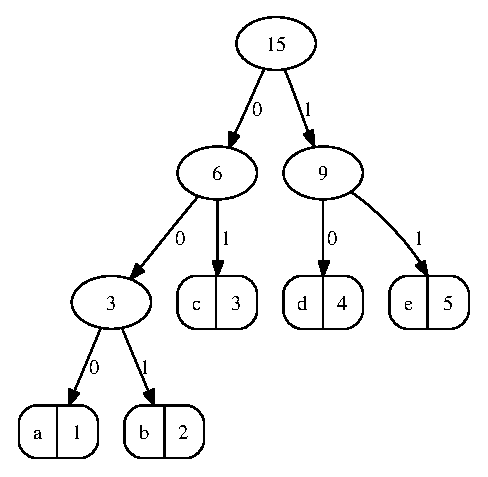
\epsfig{file=coding-tree2.eps, scale=0.7}} 
  \caption{Baum-Darstellung der Kodierung.}
  \label{fig:coding-tree2}
\end{figure}



\begin{table}[htbp]
  \centering
\begin{tabular}[t]{|l|r|r|r|r|r|}
\hline
Buchstabe &   \texttt{a} &   \texttt{b} & \texttt{c}  & \texttt{d}  & \texttt{e}   \\
\hline
Kodierung & \texttt{000} & \texttt{001} & \texttt{01} & \texttt{10} & \texttt{11} \\
\hline
\end{tabular}
  \caption{Kodierung der Buchstaben mit variabler L\"ange.}
  \label{tab:coding2}
\end{table}


\subsection{Implementierung in \textsl{Java}}
\begin{figure}[!ht]
\centering
\begin{Verbatim}[ frame         = lines, 
                  framesep      = 0.3cm, 
                  labelposition = bottomline,
                  numbers       = left,
                  numbersep     = -0.2cm,
                  xleftmargin   = 0.8cm,
                  xrightmargin  = 0.8cm,
                ]
    public abstract class Node implements Comparable<Node> {
    	public    abstract Integer cost();
    	public    abstract Integer count();
    
    	public int compareTo(Node rhs) {
    		return count().compareTo(rhs.count());
    	}
    
    }
\end{Verbatim}
\vspace*{-0.3cm}
\caption{Die abstrakte Klasse \texttt{Node}.}
\label{fig:Huffman/Node.java}
\end{figure}

\noindent
Wir zeigen nun, wie die Berechnung des Huffman-Codes in \textsl{Java} implementiert werden
kann.  Als erstes pr\"asentieren wir Klassen, um Kodierungs-B\"aume darstellen zu
k\"onnen.  Abbildung \ref{fig:Huffman/Node.java} zeigt die Implementierung der abstrakten
Klasse \texttt{Node}, mit der wir Elemente der Menge der Kodierungs-B\"aume $\mathcal{K}$ darstellen.
Da wir sp\"ater Knoten anhand der f\"ur diesen Knoten  gespeicherten H\"aufigkeiten vergleichen
m\"ussen, implementiert diese Klasse die Schnittstelle \texttt{Comparable}.
Dazu muss die Klasse \texttt{Node} die Methode $\textsl{compareTo}()$ bereitstellen.  
Diese Methode vergleicht verschiedene Knoten \"uber die Werte der Funktion $\textsl{count}()$.

\begin{figure}[!ht]
\centering
\begin{Verbatim}[ frame         = lines, 
                  framesep      = 0.3cm, 
                  labelposition = bottomline,
                  numbers       = left,
                  numbersep     = -0.2cm,
                  xleftmargin   = 0.8cm,
                  xrightmargin  = 0.8cm,
                ]
    public class LeafNode extends Node {
        private char mCharacter;
        private int  mFrequency;
        
        public LeafNode(char character, int frequency) {
            mCharacter = character;
            mFrequency = frequency;
        }
        public Integer cost() {
            return 0;
        }
        public Integer count() {
            return mFrequency;
        }
        public Character getCharacter() {
            return mCharacter;
        }
    }
\end{Verbatim}
\vspace*{-0.3cm}
\caption{Die Klasse \texttt{Leaf}.}
\label{fig:Leaf.java}
\end{figure}

Die Klasse \texttt{LeafNode} repr\"asentiert Knoten der Form $\textsl{leaf}(c,f)$.
Der Buchstabe $c$ wird in der Member-Variablen \texttt{mCharacter} abgespeichert und die H\"aufigkeit
$f$, mit der dieser Buchstabe in dem zu kodierenden String $s$ auftritt, wird in der
Member-Variablen \texttt{mFrequency} abgelegt.
\begin{enumerate}
\item Der Konstruktor initialisiert die beiden Member-Variablen \texttt{mCharacter} und
      \texttt{mFrequency}. 
\item Die Funktion $\textsl{cost}()$ liefert als Ergebnis $0$, denn f\"ur Bl\"atter hatten wir 
      \\[0.2cm]
      \hspace*{1.3cm}
      $\textsl{leaf}(c,f).\textsl{cost}() = 0$
      \\[0.2cm]
      definiert.
\item Die Funktion $\textsl{count}()$ liefert die H\"aufigkeit \texttt{mFrequency}, denn f\"ur Bl\"atter hatten wir
      \\[0.2cm]
      \hspace*{1.3cm}
      $\textsl{leaf}(c,f).\textsl{count}() = f$
      \\[0.2cm]
      definiert.
\item Die Funktion $\textsl{getCharacter}()$ gibt als Ergebnis den in der Member-Variablen \texttt{mCharacter}
      gespeicherten Buchstaben zur\"uck.
\end{enumerate}

\begin{figure}[!ht]
\centering
\begin{Verbatim}[ frame         = lines, 
                  framesep      = 0.3cm, 
                  labelposition = bottomline,
                  numbers       = left,
                  numbersep     = -0.2cm,
                  xleftmargin   = 0.8cm,
                  xrightmargin  = 0.8cm,
                ]
    public class BinaryNode extends Node {
        private Node mLeft;
        private Node mRight;
        private int  mCount;
        private int  mCost;
    
        public BinaryNode(Node left, Node right) {
            mLeft  = left;
            mRight = right;
            mCount = mLeft.count() + mRight.count();
            mCost  = mLeft.cost()  + mRight.cost() + mCount;
        }
        public Integer cost() {
            return mCost;
        }
        public Integer count() {
            return mCount;
        }
    }
\end{Verbatim}
\vspace*{-0.3cm}
\caption{Die Klasse BinaryNode.}
\label{fig:Huffman/BinaryNode.java}
\end{figure}

Die Klasse \texttt{BinaryNode} repr\"asentiert einen bin\"aren Knoten der Form
$\textsl{node}(l,r)$.  Die Klasse hat vier Member-Variablen:
\begin{enumerate}
\item \texttt{mLeft}  speichert den linken  Teilbaum $l$ des Knotens $\textsl{node}(l,r)$.
\item \texttt{mRight} speichert den rechten Teilbaum $r$ des Knotens $\textsl{node}(l,r)$.
\item \texttt{mCount} speichert den Wert der Funktion $\textsl{node}(l,r).\textsl{count}()$.
      Wir speichern diesen Wert in einer Member-Variablen, damit wir ihn nur einmal berechnen
      m\"ussen.
\item \texttt{mCost}  speichert den Wert der Funktion $\textsl{node}(l,r).\textsl{cost}()$.
\end{enumerate}
Der Konstruktor der Klasse \texttt{BinaryNode} bekommt als Argumente den linken Teilbaum $l$ und den
rechten Teilbaum $r$ des zu konstruierenden Knotens $\textsl{node}(l,r)$.  Au{\ss}erdem berechnet der
Konstruktor die Werte $\textsl{node}(l,r).\textsl{count}()$ und $\textsl{node}(l,r).\textsl{cost}()$
und speichert diese Werte in den Member-Variablen \texttt{mCount} und \texttt{mCost}.


\begin{figure}[!h]
\centering
\begin{Verbatim}[ frame         = lines, 
                  framesep      = 0.3cm, 
                  labelposition = bottomline,
                  numbers       = left,
                  numbersep     = -0.2cm,
                  xleftmargin   = 0.3cm,
                  xrightmargin  = 0.3cm,
                ]
    import java.util.*;
    import java.io.*;
    
    public class Huffman {
        Map<Character, Integer> mFrequencyTable;
        Node                    mCoding;      // the coding tree 
    
        public Huffman(String fileName) {
            determineFrequencies(fileName);
            mCoding = createHuffmanCode();
        }
        public void determineFrequencies(String fileName) {
            mFrequencyTable = new TreeMap<Character, Integer>();
            for (char c = 1; c < 128; ++c) {
                mFrequencyTable.put(c, 0);
            }
            try {
                FileReader fr = new FileReader(fileName);
                while (true) {
                    char c = (char) fr.read();
                    if (c == 65535) { break; }
                    int count = mFrequencyTable.get(c);
                    ++count;
                    mFrequencyTable.put(c, count);
                }
            } catch (IOException e) {
                e.printStackTrace();
            }
        }    
        public Node createHuffmanCode() {
            PriorityQueue<Node> queue = new PriorityQueue<Node>();
            for (Character c: mFrequencyTable.keySet()) {
                Integer frequency = mFrequencyTable.get(c);
                if (frequency >= 1) {
                    LeafNode leaf = new LeafNode(c, frequency);
                    queue.offer(leaf);
                }
            }
            while (queue.size() > 1) {
                Node left  = queue.remove();
                Node right = queue.remove();
                Node node  = new BinaryNode(left, right);
                queue.offer(node);
            }
            return queue.peek();
        }
    }
\end{Verbatim}
\vspace*{-0.3cm}
\caption{Die Klasse Huffman.}
\label{fig:Huffman.java}
\end{figure}

Die Abbildung \ref{fig:Huffman.java} auf Seite \pageref{fig:Huffman.java} zeigt die
Implementierung der Klasse \texttt{Huffman}, die f\"ur einen gegebenen String den
Huffman-Code berechnet. 
Die Klasse \texttt{Huffman} enth\"alt zwei Member-Variablen:
\begin{enumerate}
\item \texttt{mFrequencyTable} ist eine Abbildung, die f\"ur jeden Buchstaben $c$, der in
      der gegebenen Datei auftritt, angibt, wie oft dieser Buchstabe in der Datei auftritt.
\item \texttt{mCoding} ist ein Knoten der Form $\textsl{node}(l,r)$.  Dieser Knoten ist
      das Endergebnis der Berechnung und enth\"alt den Kodierungs-Baum f\"ur den
      gegebenen Text.
\end{enumerate}
Wir besprechen jetzt die Details der Implementierung des Konstruktors und der Methoden in der Klasse
Huffman.
\begin{enumerate}
\item Der Konstruktor der Klasse \texttt{Huffman} bekommt als Argument den Namen der Datei, die
      den Text enth\"alt, f\"ur den der Huffman-Code bestimmt werden soll.  Anschlie{\ss}end liest
      die Methode $\textsl{determineFrequencies}()$  die angegebene Datei und berechnet die H\"aufigkeiten,
      mit denen die einzelnen Buchstaben auftreten.  Diese H\"aufigkeiten dann werden in der
      Tabelle \texttt{mFrequencyTable} abgespeichert.  Daraus berechnet die Methode
      $\textsl{createHuffmanCode}()$ den Huffman-Code mit Hilfe dieser Tabelle.
\item Die Methode $\textsl{determineFrequencies}()$ geht davon aus, dass als Zeichen nur
      Buchstaben aus dem \textsc{Ascii}-Zeichensatz verwendet werden.
      \begin{enumerate}
      \item Zun\"achst wird daher eine Tabelle f\"ur die 127 Zeichen aus dem
            \textsc{Ascii}-Zeichensatz angelegt.   Diese Tabelle soll jedem 
            Buchstaben die H\"aufigkeit, mit der dieser Buchstabe in der Datei auftritt,
            zuordnen.  Die Eintr\"age dieser Tabelle werden 
            in der \texttt{for}-Schleife in Zeile 15 zun\"achst mit 0 initialisiert.
            Sp\"ater wird jedes Mal,  wenn wir einen Buchstaben lesen, die dem Buchstaben
            zugeordnete H\"aufigkeit inkrementiert.
      \item Anschlie{\ss}end wir die Datei in Zeile 18 zum Lesen ge\"offnet.
      \item In der anschlie{\ss}enden \texttt{while}-Schleife wird die Datei zeichenweise
            gelesen.  Falls dabei das Datei-Ende-Zeichen \texttt{EOF} gelesen wird,
            bricht diese Schleife durch den \texttt{break}-Befehl in Zeile 21 ab. 
            
            Wurde ein Zeichen $c$ gelesen, so wird zun\"achst in der Tabelle
            \texttt{mFrequencyTable} nachgeschlagen, wie h\"aufig dieses Zeichen schon
            aufgetreten ist.  Diese Zahl wird um 1 inkrementiert und die inkrementierte
            Zahl wird wieder in die Tabelle zur\"uckgeschrieben.
            
            Da die IO-Operationen in Zeile 18 und Zeile 20 Ausnahmen ausl\"osen k\"onnen,
            m\"ussen diese Anweisungen in einem \texttt{try}-\texttt{catch}-Block eingerahmt
            werden.
      \end{enumerate}
\item Die Methode $\textsl{createHuffmanCode}()$ implementiert den Algorithmus von Huffman.
      \begin{enumerate}
      \item Zun\"achst wird in Zeile 31 eine neue Priorit\"ats-Warteschlange angelegt.
      \item In der \texttt{for}-Schleife in Zeile 32 iterieren wir \"uber alle Zeichen.
            Falls ein Zeichen mindestens einmal in dem Text vorkommt,
            erzeugen wir in Zeile 35 einen Knoten $\textsl{leaf}(c,f)$ und f\"ugen diesen
            Knoten der Priorit\"ats-Warteschlange hinzu.
      \item Die \texttt{while}-Schleife in Zeile 39 implementiert den Pseudo-Code aus 
            Abbildung \ref{fig:huffman}:  Wir entfernen die beiden Knoten $l$ und $r$ mit den
            niedrigsten Priorit\"aten aus der Priorit\"ats-Warteschlange und bilden den neuen
            Knoten $\textsl{node}(l,r)$, den wir stattdessen in die
            Priorit\"ats-Warteschlange einf\"ugen.  Wenn die Priorit\"ats-Warteschlange nur noch
            genau einen Knoten enth\"alt, sind wir am Ziel und geben diesen Knoten 
            als Ergebnis zur\"uck.
      \end{enumerate}
\end{enumerate}

\noindent
\textbf{Aufgabe}:
\begin{enumerate}
\item Berechnen Sie den Huffman-Code f\"ur einen Text, der nur die Buchstaben
      ``\texttt{a}'' bis ``\texttt{g}'' enth\"alt und f\"ur den die H\"aufigkeiten,
      mit denen diese Buchstaben auftreten, durch die folgende Tabelle gegeben sind.

\begin{table}[htbp]
  \centering
\begin{tabular}[t]{|l|r|r|r|r|r|r|r|}
\hline
Buchstabe  & \texttt{a} & \texttt{b} & \texttt{c} & \texttt{d} & \texttt{e} & \texttt{f} & \texttt{g} \\
\hline
H\"aufigkeit &          1 &          1 &          2 &          3 &          5 &         8 &         13 \\
\hline
\end{tabular}
  \caption{Buchstaben mit H\"aufigkeiten.}
  \label{tab:aufgabe-huffman}
\end{table}

\item Wie gro{\ss} ist die Einsparung, wenn man die Buchstaben mit einem Huffman-Code
      kodiert gegen\"uber einer Kodierung mit drei Bits?
\item Versuchen Sie das Gesetz zu erkennen, nach dem die H\"aufigkeiten in der obigen Tabelle 
      gebildet wurden und versuchen Sie, den Huffman-Code f\"ur den allgemeinen Fall,
      in dem $n$ Buchstaben gegeben sind, anzugeben.
\item Wie gro{\ss} ist die Einsparung im allgemeinen Fall?
\end{enumerate}

\section{Optimalit\"at des Huffman'schen Kodierungsbaums}
In diesem Abschnitt zeigen wir, dass der durch den Algorithmus von Huffman berechnete Kodie\-rungs-Baum der
Kodierungs-Baum ist, f\"ur den die Funktion $\textsl{cost}()$ minimal ist.  Dazu geben zun\"achst eine andere
Formel zur Berechnung von $n.\textsl{cost}()$ an:  Wir definieren die \emph{Tiefe}
$n.\textsl{depth}(c)$ des Buchstabens $c$ in dem Kodierungs-Baum $n$ als den Abstand, den das Blatt $l$,
das mit dem Buchstaben $c$ markiert ist, von der Wurzel des Kodierungs-Baums hat.  Der Kodierungs-Baum
wird dabei als Graph aufgefasst.  Dann gibt es genau einen Pfad von der Wurzel zu dem Blatt $l$ und 
$n.\textsl{depth}(c)$ wird als die Anzahl der Kanten dieses Pfades definiert.
Jede der Kanten dieses Pfades tr\"agt hinterher ein Bit zur 
Kodierung des Buchstabens bei, mit dem das Blatt $l$ markiert ist.  Um die gesamten Kosten zu berechnen
m\"ussen wir daher die Tiefe jedes Buchstabens mit seiner H\"aufigkeit multiplizieren.  Bezeichnen wir die
H\"aufigkeit des Buchstabens $c$ mit $\textsl{freq}(c)$, so erhalten wir insgesamt
\begin{equation}
  \label{eq:cost}
  n.\textsl{cost}() = \sum\limits_{c\in\Sigma} \textsl{freq}(c) \cdot n.\textsl{depth}(c)
\end{equation}
Die Summe l\"auft dabei \"uber alle Buchstaben des Alphabets $\Sigma$, wobei wir voraussetzen,
dass alle Buchstaben aus $\Sigma$ auch tats\"achlich in dem Kodierungs-Baum auftreten.
Buchstaben, die gar nicht auftreten, werden also vorher aus dem Alphabet entfernt.

\begin{Definition}[Optimaler Kodierungs-Baum]
  Ein Kodierungs-Baum $n$ ist \emph{optimal}, wenn bei gegebener H\"aufigkeit der Buchstaben
  der Wert $n.\textsl{cost}()$ minimal ist, f\"ur alle Kodierungs-B\"aume $k$, bei denen die
  Buchstaben mit derselben H\"aufigkeit auftreten wie in $n$,  gilt also
  \\[0.2cm]
  \hspace*{1.3cm} $n.\textsl{cost}() \leq k.\textsl{cost}()$.
\end{Definition}


\begin{Lemma}
  \label{huffman:l1}
  Es seien $x$ und $y$ die beiden Buchstaben aus dem Alphabet $\Sigma$ mit der geringsten H\"aufigkeit.  Dann
  gibt es einen optimalen Kodierungs-Baum $n$, bei dem sich die Kodierung der Buchstaben $x$ und $y$ nur im
  letzten Bit unterscheidet.
\end{Lemma}

\noindent
\textbf{Beweis}:  Es sei $n_1$ ein optimaler Kodierungs-Baum.  Wir zeigen, wie $n_1$ zu einem
Kodierungs-Baum $n_2$ umgebaut werden kann, der einerseits optimal ist und bei dem sich andererseits die
Kodierung der Buchstaben $x$ und $y$ nur im letzten Bit unterscheidet.  Wir suchen in dem Kodierungs-Baum
$n_1$ einen Knoten $k$ der Form $\textsl{node}(l,r)$, der unter allen \emph{inneren} Knoten eine maximale
Tiefe hat.  Dabei bezeichnen wir alle Knoten, die keine Bl\"atter sind, als innere Knoten.
An dem Knoten $k$ h\"angen zwei Buchstaben $a$ und $b$.  Wir machen nun o.B.d.A.~die folgenden Annahmen
\"uber die H\"aufigkeiten der Buchstaben:
\begin{enumerate}
\item $\textsl{freq}(x) \leq \textsl{freq}(y)$,
\item $\textsl{freq}(a) \leq \textsl{freq}(b)$.
\end{enumerate}
Da wir angenommen haben, dass $x$ und $y$ die Buchstaben mit der geringsten H\"aufigkeiten sind, folgt
daraus
\begin{equation}
  \label{eq:huffmannL0}
\textsl{freq}(x) \leq \textsl{freq}(a) \quad \textrm{und} \quad 
\textsl{freq}(y) \leq \textsl{freq}(b).  
\end{equation}
Wir erhalten nun den Kodierungs-Baum $n_2$ aus dem Kodierungs-Baum $n_1$, indem wir in dem Baum $n_1$ die
Positionen der Buchstaben $x$ und $a$ und die Positionen der Buchstaben $y$ und $b$ vertauschen.
Daher gilt 
  \begin{eqnarray}
    \label{eq:huffmannL1a}
 n_2.\textsl{depth}(a) &=& n_1.\textsl{depth}(x), \\
    \label{eq:huffmannL1b}
 n_2.\textsl{depth}(b) &=& n_1.\textsl{depth}(y), \\
    \label{eq:huffmannL1c}
 n_2.\textsl{depth}(x) &=& n_1.\textsl{depth}(a), \\
    \label{eq:huffmannL1d}
 n_2.\textsl{depth}(y) &=& n_1.\textsl{depth}(b).
  \end{eqnarray}
denn $a$ und $x$ und $b$ und $y$ vertauschen die Pl\"atze.  F\"ur alle Buchstaben
$c \in \Sigma\backslash\{a,b,x,y\}$ gilt nat\"urlich 
\begin{equation}
  \label{eq:huffmannL1e}
n_2.\textsl{depth}(c) = n_1.\textsl{depth}(c).   
\end{equation}
Weiterhin wissen wir aufgrund der Auswahl des Knotens $k$, dass
\begin{eqnarray}
  \label{eq:huffmannL2a}
  n_1.\textsl{depth}(a) = n_1.\textsl{depth}(b) \geq n_1.\textsl{depth}(x) \quad \mathrm{und} \\
  \label{eq:huffmannL2b}
  n_1.\textsl{depth}(a) = n_1.\textsl{depth}(b) \geq n_1.\textsl{depth}(y) \hspace*{0.95cm}
\end{eqnarray}
gilt.  Wir zeigen nun, dass $n_2.\textsl{cost}() \leq n_1.\textsl{cost}()$ gilt.  Dazu geben wir zun\"achst
$n_2.\textsl{cost}()$ an.
\begin{eqnarray*}
  n_2.\textsl{cost}() 
  & = & \sum\limits_{c\in\Sigma} \textsl{freq}(c) \cdot n_2.\textsl{depth}(c) \\
  & = & \sum\limits_{c\in\Sigma\backslash\{a,b,x,y\}} \textsl{freq}(c) \cdot n_2.\textsl{depth}(c) \\[0.3cm]
  &   & + \;\textsl{freq}(a) \cdot n_2.\textsl{depth}(a) 
        + \textsl{freq}(b) \cdot n_2.\textsl{depth}(b) \\[0.1cm]
  &   & + \;\textsl{freq}(x) \cdot n_2.\textsl{depth}(x) 
        + \textsl{freq}(y) \cdot n_2.\textsl{depth}(y) 
\end{eqnarray*}
Unter Ber\"ucksichtigung der Gleichungen (\ref{eq:huffmannL1a}) bis (\ref{eq:huffmannL1e}) k\"onnen wir dies
auch schreiben als
\begin{eqnarray*}  
  n_2.\textsl{cost}() 
  & = & \sum\limits_{c\in\Sigma\backslash\{a,b,x,y\}} \textsl{freq}(c) \cdot n_1.\textsl{depth}(c) \\[0.3cm]
  &   & + \;\textsl{freq}(a) \cdot n_1.\textsl{depth}(x) 
        + \textsl{freq}(b) \cdot n_1.\textsl{depth}(y) \\[0.1cm]
  &   & + \;\textsl{freq}(x) \cdot n_1.\textsl{depth}(a) 
        + \textsl{freq}(y) \cdot n_1.\textsl{depth}(b) 
\end{eqnarray*}
Analog berechnen wir $n_1.\textsl{cost}()$:
\begin{eqnarray*}
  n_1.\textsl{cost}() 
  & = & \sum\limits_{c\in\Sigma} \textsl{freq}(c) \cdot n_1.\textsl{depth}(c) \\
  & = & \sum\limits_{c\in\Sigma\backslash\{a,b,x,y\}} \textsl{freq}(c) \cdot n_1.\textsl{depth}(c) \\[0.3cm]
  &   & + \;\textsl{freq}(a) \cdot n_1.\textsl{depth}(a) 
        + \textsl{freq}(b) \cdot n_1.\textsl{depth}(b) \\[0.1cm]
  &   & + \;\textsl{freq}(x) \cdot n_1.\textsl{depth}(x) 
        + \textsl{freq}(y) \cdot n_1.\textsl{depth}(y) 
\end{eqnarray*}
Damit sehen wir, dass $n_2.\textsl{cost}() \leq n_1.\textsl{cost}()$ genau dann gilt, wenn die
Ungleichung 
\\[0.2cm]
\hspace*{0.8cm}
$\textsl{freq}(a) \cdot n_1.\textsl{depth}(x) 
      + \textsl{freq}(b) \cdot n_1.\textsl{depth}(y) 
      + \textsl{freq}(x) \cdot n_1.\textsl{depth}(a) 
      + \textsl{freq}(y) \cdot n_1.\textsl{depth}(b)$ \\[0.1cm]
\hspace*{0.3cm}
$\leq\; \textsl{freq}(a) \cdot n_1.\textsl{depth}(a) 
      + \textsl{freq}(b) \cdot n_1.\textsl{depth}(b) 
      + \textsl{freq}(x) \cdot n_1.\textsl{depth}(x) 
      + \textsl{freq}(y) \cdot n_1.\textsl{depth}(y)$ \\[0.2cm]
erf\"ullt ist.  Da in dieser Ungleichung nur noch der Knoten $n_1$ vorkommt, vereinfachen wir die
Schreibweise und vereinbaren, dass wir einen Ausdruck der Form $n_1.\textsl{depth}(u)$ zu
$\textsl{depth}(u)$ abk\"urzen.  Die letzte Ungleichung ist dann \"aquivalent zu der Ungleichung
\\[0.2cm]
\hspace*{0.8cm}
$0 \;\leq\; \textsl{freq}(a) \cdot \bigl(\textsl{depth}(a) - \textsl{depth}(x)\bigr)
          + \textsl{freq}(b) \cdot \bigl(\textsl{depth}(b) - \textsl{depth}(y)\bigr)$ 
\\[0.2cm]
\hspace*{1.3cm}
$        -\;\textsl{freq}(x) \cdot \bigl(\textsl{depth}(a) - \textsl{depth}(x)\bigr) 
         - \textsl{freq}(y) \cdot \bigl(\textsl{depth}(b) - \textsl{depth}(y)\bigr)$ \\[0.2cm]
Diese Ungleichung vereinfachen wir zu 
\\[0.3cm]
\hspace*{0.3cm}
$0 \;\leq\; 
  \underbrace{\bigl(\textsl{freq}(a) - \textsl{freq}(x)\bigr)}_{\geq 0}   \cdot 
  \underbrace{\bigl(\textsl{depth}(a) - \textsl{depth}(x)\bigr)}_{\geq 0}
+ \underbrace{\bigl(\textsl{freq}(b) - \textsl{freq}(y)\bigr)}_{\geq 0}   \cdot 
  \underbrace{\bigl(\textsl{depth}(b) - \textsl{depth}(y)\bigr)}_{\geq 0}$
\\[0.3cm]
Hier gilt $\textsl{freq}(a) - \textsl{freq}(x) \geq 0$ wegen Ungleichung \ref{eq:huffmannL0},
die Ungleichung $\textsl{depth}(a) - \textsl{depth}(x) \geq 0$ folgt aus Ungleichung \ref{eq:huffmannL2a},
die Ungleichung $\textsl{freq}(b) - \textsl{freq}(y) \geq 0$ folgt aus Ungleichung \ref{eq:huffmannL0}
und die Ungleichung $\textsl{depth}(b) - \textsl{depth}(y) \geq 0$ 
folgt aus Ungleichung \ref{eq:huffmannL2b}.
Damit haben wir 
\[ n_2.\textsl{cost}() \leq n_1.\textsl{cost}() \]
gezeigt.  Da $n_1$ optimal ist, muss auch $n_2$ optimal sein.  Nach Wahl des Knotens $k$ unterscheiden
sich die Kodierungen von $x$ und $y$ nur in dem letzten Bit. Damit ist $n_2$ der gesuchte
Kodierungs-Baum.
\hspace*{\fill} $\Box$

\begin{Satz}
  Der Kodierungs-Baum, der von dem Huffman-Algorithmus erzeugt wird, ist optimal.
\end{Satz}

\noindent
\textbf{Beweis}:  Wir beweisen den Satz durch Induktion \"uber die Anzahl $n$ der Buchstaben in dem
Alphabet $\Sigma$.
\begin{enumerate}
\item[I.A.:] $n = 2$.  Es sei $\Sigma= \{a,b\}$.
  In diesem Fall f\"uhrt der Huffman-Algorithmus nur einen Schritt durch und liefert den Kodierungs-Baum 
  \\[0.2cm]
  \hspace*{1.3cm}
  $k=\textsl{node}\bigl(\textsl{leaf}(a, \textsl{freq}(a)), \textsl{leaf}(b,\textsl{freq}(b))\bigr)$.
  \\[0.2cm]
  Bei der Kodierung eines Alphabets, das aus zwei Buchstaben besteht, haben wir keine Wahl, 
  was die L\"ange der Kodes angeht: Wir brauchen f\"ur jeden Buchstaben genau ein Bit und daher ist das vom
  Huffman-Algorithmus in diesem Fall gelieferte Ergebnis offenbar optimal.
\item[I.S.:] $n \mapsto n+1$

  Wir gehen jetzt davon aus, dass das Alphabet $\Sigma$ aus $n+1$ Buchstaben besteht.
  Es seien $x$ und $y$ die beiden Buchstaben, deren H\"aufigkeit minimal ist.
  Es sei $z$ ein neuer Buchstabe, der nicht in dem Alphabet $\Sigma$ auftritt.  Wir definieren
  ein neues Alphabet $\Sigma'$ als
  \\[0.2cm]
  \hspace*{1.3cm}
  $\Sigma' = \bigl(\Sigma \backslash \{x,y\}\bigr) \cup \{z\}$.
  \\[0.2cm]
  Die H\"aufigkeit des neuen Buchstabens $z$ definieren wir als 
  \\[0.2cm]
  \hspace*{1.3cm}
  $\textsl{freq}(z) := \textsl{freq}(x) + \textsl{freq}(y)$.
  \\[0.2cm]
  Dann enth\"alt das Alphabet $\Sigma'$ insgesamt $n$ Buchstaben.  Wenden wir den Huffman-Algorithmus
  auf dieses Alphabet an, so erhalten wir nach Induktions-Voraussetzung f\"ur $\Sigma'$ einen optimalen
  Kodierungs-Baum $k_1$.  Die Anwendung des Huffman-Algorithmus auf das Alphabet $\Sigma$ ersetzt in diesem
  Kodierungs-Baum das Blatt, das mit dem Buchstaben $z$ markiert ist, durch den Knoten 
  \\[0.2cm]
  \hspace*{1.3cm}
  $\textsl{node}\bigl(\textsl{leaf}(x, \textsl{freq}(x)), \textsl{leaf}(y,\textsl{freq}(y))\bigr)$.
  \\[0.2cm]
  Bezeichnen wir den so entstanden Kodierungs-Baum mit $k_2$, so m\"ussen wir zeigen, dass $k_2$ optimal
  ist.  Wir f\"uhren den Beweis indirekt und nehmen an, dass $k_2$ nicht optimal ist. Dann gibt es einen
  Kodierungs-Baum $k_3$ f\"ur das Alphabet $\Sigma$, so dass 
  \\[0.2cm]
  \hspace*{1.3cm}
  $k_3.\textsl{cost}() < k_2.\textsl{cost}()$
  \\[0.2cm]
  ist.  Nach Lemma \ref{huffman:l1} k\"onnen wir o.B.d.A. voraussetzen, dass sich die Kodierung der 
  Buchstaben $x$ und $y$ in dem Kodierungs-Baum $k_3$ nur in dem letzten Bit
  unterscheidet.  Also gibt es in dem Kodierungs-Baum $k_3$ einen Knoten der Form
  \\[0.2cm]
  \hspace*{1.3cm}
  $\textsl{node}\bigl(\textsl{leaf}(x, \textsl{freq}(x)), \textsl{leaf}(y,\textsl{freq}(y))\bigr)$.
  \\[0.2cm]
  Wir transformieren den Kodierungs-Baum $k_3$ in einen Kodierungs-Baum $k_4$ f\"ur das Alphabet $\Sigma'$ indem
  wir diesen Knoten durch das Blatt
  \\[0.2cm]
  \hspace*{1.3cm}
  $\textsl{leaf}\bigl(z, \textsl{freq}(x) + \textsl{freq}(y)\bigr)$
  \\[0.2cm]
  ersetzen.  Damit gilt
  \begin{eqnarray*}
      k_4.\textsl{cost}() 
  &=& \sum\limits_{c\in\Sigma'} \textsl{freq}(c) \cdot k_4.\textsl{depth}(c) \\[0.3cm]
  &=& \sum\limits_{c\in\Sigma\backslash\{x,y\}\cup\{z\}} \textsl{freq}(c) \cdot k_4.\textsl{depth}(c) 
      \\[0.3cm]
  &=& \sum\limits_{c\in\Sigma\backslash\{x,y\}} \textsl{freq}(c) \cdot k_4.\textsl{depth}(c) 
      +\textsl{freq}(z) \cdot k_4.\textsl{depth}(z) \\[0.3cm]  
  &=& \sum\limits_{c\in\Sigma\backslash\{x,y\}} \textsl{freq}(c) \cdot k_3.\textsl{depth}(c) 
      +\textsl{freq}(z) \cdot \bigl(k_3.\textsl{depth}(x) - 1\bigr) \\[0.3cm]  
  &=& \sum\limits_{c\in\Sigma\backslash\{x,y\}} \textsl{freq}(c) \cdot k_3.\textsl{depth}(c) \\[0.3cm]
  & & +\; \bigl(\textsl{freq}(x) + \textsl{freq}(y)\bigr) \cdot \bigl(k_3.\textsl{depth}(x) - 1\bigr) 
      \\[0.3cm]  
  &=& \sum\limits_{c\in\Sigma} \textsl{freq}(c) \cdot k_3.\textsl{depth}(c) -\; \bigl(\textsl{freq}(x) + \textsl{freq}(y)\bigr)  
      \\[0.3cm]  
  &=& k_3.\textsl{cost}() - \bigl(\textsl{freq}(x) + \textsl{freq}(y)\bigr)  
  \end{eqnarray*}
  Wir halten dieses Ergebnis in einer Gleichung fest:
  \begin{equation}
    \label{eq:huffmanns1}
    k_4.\textsl{cost}() = k_3.\textsl{cost}() - \bigl(\textsl{freq}(x) + \textsl{freq}(y)\bigr).
  \end{equation}
  Da die Kodierungs-B\"aume $k_1$ und $k_2$ in derselben Relation stehen wie die Kodierungs-B\"aume
  $k_4$ und $k_3$, gilt analog
  \begin{equation}
    \label{eq:huffmanns2}
    k_1.\textsl{cost}() = k_2.\textsl{cost}() - \bigl(\textsl{freq}(x) + \textsl{freq}(y)\bigr). 
  \end{equation}
  Damit k\"onnen wir zeigen, dass die Kosten des Kodierungs-Baums $k_4$ geringer sind als die Kosten
  des Kodierungs-Baums $k_1$:
  \begin{eqnarray*}
         k_4.\textsl{cost}() 
   & = & k_3.\textsl{cost}() - \bigl(\textsl{freq}(x) + \textsl{freq}(y)\bigr) \\[0.1cm]
   & < & k_2.\textsl{cost}() - \bigl(\textsl{freq}(x) + \textsl{freq}(y)\bigr) \\[0.1cm] 
   & = & k_1.\textsl{cost}(). 
  \end{eqnarray*}
  Dieses Ergebnis steht aber im Widerspruch dazu, dass der Kodierungs-Baum $k_1$ 
  optimal ist.  Folglich ist die Annahme $k_3.\textsl{cost}() < k_2.\textsl{cost}()$ falsch und der
  Kodierungs-Baum $k_2$ ist bereits optimal.
  \hspace*{\fill} $\Box$
\end{enumerate}


%%% Local Variables: 
%%% mode: latex
%%% TeX-master: "algorithmen"
%%% End: 

\chapter{Graphentheorie}
Wir wollen zum Abschluss der Vorlesung wenigstens ein graphentheoretisches Problem
vorstellen: Das Problem der Berechnung  k\"urzester Wege. 


\section{Die Berechnung k\"urzester Wege}
Um das Problem der Berechnung k\"urzester Wege formulieren zu k\"onnen, f\"uhren wir zun\"achst 
den Begriff des \emph{gewichteten Graphen} ein.  

\begin{Definition}[Gewichteter Graph]
{\em
  Ein  {\em gewichteter Graph} ist ein Tripel
   $\langle \nodes, \edges, \weight{\cdot} \rangle$ so dass gilt:
  \begin{enumerate}
  \item $\nodes$ ist eine Menge von \emph{Knoten}.
  \item $\edges \subseteq \nodes \times \nodes$ ist eine Menge von \emph{Kanten}.
  \item $\weight{\cdot}: \edges \rightarrow \N \backslash\{0\}$ ist eine Funktion,
        die jeder Kante eine positive \emph{L\"ange} zuordnet.
        \conclude
  \end{enumerate}
}
\end{Definition}

\noindent
Ein \emph{Pfad} $P$ ist eine Liste der Form \\[0.2cm]
\hspace*{1.3cm} $P = [ x_1, x_2, x_3, \cdots, x_n ]$ \\[0.2cm]
so dass f\"ur alle $i = 1, \cdots, n-1$ gilt: \\[0.2cm]
\hspace*{1.3cm} $\pair(x_i,x_{i+1}) \in \edges$. \\[0.2cm]
Die Menge aller Pfade bezeichnen wir mit $\paths$.
Die L\"ange eines Pfads definieren wir als die Summe der L\"ange aller Kanten:
\\[0.2cm]
\hspace*{1.3cm} $\Weight{[x_1,x_2, \cdots, x_n]} \df \sum\limits_{i=1}^{n-1} \Weight{\pair(x_i,x_{i+1})}$. \\[0.2cm]
Ist $p = [x_1, x_2, \cdots, x_n]$ ein Pfad, so sagen wir, dass $p$ den Knoten $x_1$ mit dem
Knoten $x_n$ verbindet.   Die Menge alle Pfade, die den Knoten $v$ mit dem Knoten $w$
verbinden, bezeichnen wir als \\[0.2cm]
\hspace*{1.3cm} 
 $\paths(v,w) \df \bigl\{ [x_1, x_2, \cdots, x_n] \in \paths \mid x_1 = v \,\wedge\, x_n = w \}$.
\\[0.2cm]
Damit k\"onnen wir nun das Problem der Berechnung k\"urzester Wege formulieren.
\begin{Definition}[K\"urzeste-Wege-Problem]
{\em
  Gegeben sei ein gewichteter Graph $G = \langle \nodes, \edges, \weight{\cdot} \rangle$ 
  und ein  Knoten $\source \in \nodes$.  Dann besteht das 
  {\em k\"urzeste-Wege-Problem}  darin, die folgende Funktion zu berechnen: \\[0.2cm]
  \hspace*{1.3cm} $\spath: \nodes \rightarrow \N$ \\[0.1cm]
  \hspace*{1.3cm} $\spath(v) \df \mathtt{min}\bigl\{ \weight{p} \mid p \in \paths(\source,v) \bigr\}$.
  \conclude  
}
\end{Definition}

\subsection{Ein naiver Algorithmus zur L\"osung des k\"urzeste-Wege-Problems}
Als erstes betrachten wir einen ganz naiven Algorithmus zur L\"osung des k\"urzeste-Wege-Problems.
Die Idee ist, dass wir eine Funktion \\[0.2cm]
\hspace*{1.3cm} $\texttt{dist}: \nodes \rightarrow \N \cup \{\Omega\}$ \\[0.2cm]
definieren, die f\"ur einen Punkt $u \in \nodes$ eine obere Absch\"atzung des Abstandes zum Knoten
\textsl{source} angibt, es soll also immer gelten: \\[0.2cm]
\hspace*{1.3cm} $\textsl{dist}(u) \not= \Omega \;\rightarrow\; \spath(u) \leq
\textsl{dist}(u)$. \\[0.2cm]
Die Funktion \textsl{dist} liefert zu einem Knoten $x$ die k\"urzeste bisher
bekannte Entfernung zum Knoten \textsl{source}.  Solange noch kein Pfad von
\textsl{source} zu dem Knoten $u$ gefunden worden ist, gilt $\textsl{dist}(u) = \Omega$.
Anfangs ist die Funktion $\textsl{dist}()$ also nur f\"ur den Knoten \textsl{source}
definiert, es gilt \\[0.2cm]
\hspace*{1.3cm} $\textsl{dist}(\textsl{source}) = 0$. \\[0.2cm]
Sp\"ater, wenn wir f\"ur einen Knoten $u$ einen Pfad gefunden haben, der den Knoten
\textsl{source} mit dem Knoten $u$ verbindet und wenn es zus\"atzlich eine Kante
$\pair(u,v)$ gibt, die den Knoten $u$ mit einem anderen Knoten $v$ verbindet, dann wissen
wir, dass auch der Knoten $v$ von \textsl{source} erreichbar ist.  Zus\"atzlich wissen wir,
dass dieser Weg die L\"ange $\textsl{dist}(u) + \weight{\pair(u,v)}$ hat.  Falls bisher also
$\textsl{dist}(v)$ undefiniert war, weil wir noch keinen Weg gefunden hatten, der
\textsl{source} mit $v$ verbindet, k\"onnen wir \\
\hspace*{1.3cm} $\textsl{dist}(v) := \textsl{dist}(u) + \weight{\pair(u,v)}$ \\[0.2cm]
setzen.  Diese Zuweisung ist ebenfalls g\"ultig wenn $\textsl{dist}(v)$ bereits definiert
ist aber einen Wert hat, der gr\"o{\ss}er als $\textsl{dist}(u) + \weight{\pair(u,v)}$ ist.
Wir fassen diese Überlegungen in den beiden
\textsl{ASM}-Regeln zusammen, die in Abbildung \ref{fig:rule-naive} dargestellt sind.  
Die Abk\"urzung \textsc{ASM} steht f\"ur \emph{abstract state machine}.
Dieser Begriff wurde von 
Yuri Gurevich \cite{gurevich:91} eingef\"uhrt und von Egon B\"orger \cite{boerger:2003} zur
Spezifikation und Verifikation von 
Algorithmen  propagiert und weiterentwickelt.  ASMs sind eine Art Pseudo-Code.  Die 
wesentlichen Eigenschaften von ASMs sind wie folgt:
\begin{enumerate}
\item ASMs bestehen aus Regeln.  Dabei besteht jede Regel
      aus einem Namen, einer Bedingung und einer Menge von Zuweisungen.
\item Bei der Abarbeitung der Regeln wird willk\"urlich eine Regel ausgew\"ahlt, deren
      Bedingung wahr ist und die Zuweisungen dieser Regel werden ausgef\"uhrt.
\item Bei Zuweisungen k\"onnen nicht nur Variablen ge\"andert werden, sondern es k\"onnen auch die Werte,
      die eine Funktion an einer Stelle annimmt, ver\"andert werden k\"onnen.  Eine Zuweisung
      kann also die Form
      \\[0.2cm]
      \hspace*{1.3cm}
      $f(x) := y$
      \\[0.2cm]
      haben.  Diese Zuweisung \"andert die Funktion $f$ so ab, dass die Funktion anschlie{\ss}end an der Stelle $x$
      den Wert $y$ annimmt.
\item Wenn es keine Regel mehr gibt, deren Bedingung wahr ist, dann h\"alt die ASM an.
\item Die Zuweisungen einer Regel werden alle gleichzeitig ausgef\"uhrt.  In der Regel 
      \\[0.2cm]
      \hspace*{0.8cm} \texttt{\underline{Rule}} \textsl{swap}            \\
      \hspace*{1.3cm} \texttt{\underline{if} x < y \underline{then}}     \\
      \hspace*{1.8cm} \texttt{x := y;}                                   \\
      \hspace*{1.8cm} \texttt{y := x;}                                   \\
      \hspace*{1.3cm} \texttt{\underline{endif}}                         \\[0.2cm]
      werden die beiden Zuweisungen also gleichzeitig ausgef\"uhrt, so dass im Endeffekt die
      Werte von \texttt{x} und \texttt{y} vertauscht werden.
\end{enumerate}
Wie ASMs im Detail funktionieren, erkl\"aren wir bei der Diskussion des in Abbildung
\ref{fig:rule-naive} gegebenen Beispiels.

\begin{figure}[!ht]
  \centering
\begin{Verbatim}[ frame         = lines, 
                  framesep      = 0.3cm, 
                  labelposition = bottomline,
                  numbers       = left,
                  numbersep     = -0.2cm,
                  commandchars  = \\\{\},
                  xleftmargin   = 0.0cm,
                  xrightmargin  = 0.0cm
                ]
    \underline{Rule} \textsl{Init}
        \underline{if}  \(\textsl{dist}(\textsl{source}) = \Omega\)
        \underline{then}
            \(\textsl{dist}(\textsl{source})\) := \(0\);
        \underline{endif}
        
    \underline{Rule} \textsl{Run}
        \underline{if} \underline{choose} \(\langle{}u,v\rangle\in\edges\) \underline{satisf}y\underline{in}g
            \(\textsl{dist}(u) \not= \Omega\) \underline{and}  \((\textsl{dist}(v) = \Omega\) \underline{or} \(\textsl{dist}(u)+\weight{\langle{}u,v\rangle}<\textsl{dist}(v))\)
        \underline{then}
            \(\textsl{dist}(v)\) := \(\textsl{dist}(u)+\weight{\langle{}u,v\rangle}\);
        \underline{endif}
\end{Verbatim}
\vspace*{-0.3cm}
  \caption{ASM-Regeln zur L\"osung des k\"urzeste-Wege-Problems.}
  \label{fig:rule-naive}
\end{figure} 
\begin{enumerate}
\item Die erste Regel hat den Namen \textsl{Init}.
      In dieser Regel wird  $\textsl{dist}(\textsl{source})$ auf den Wert 0
      gesetzt, wenn die Funktion \textsl{dist} an der Stelle \textsl{source}
      noch undefiniert ist.  Diese Regel kann nur einmal ausgef\"uhrt werden,
      denn nach Ausf\"uhrung der Regel ist $\textsl{dist}(source)$ von $\Omega$ verschieden.
\item Die zweite Regel benutzt das Konstrukt \texttt{choose}.
      Dieses Konstrukt hat allgemein die Form 
      \\[0.2cm]
      \hspace*{1.3cm}
      \texttt{choose} $\langle x_1, \cdots, x_n\rangle \in M: F(x_1,\cdots,x_n)$
      \\[0.2cm]
      Hierbei sind $x_1, \cdots, x_n$ verschiedene Variablen, $M$ ist eine Menge von
      $n$-Tupeln und \linebreak 
      $F(x_1,\cdots,x_n)$ ist eine
      logische Formel, in der diese Variablen auftreten.
      Das \texttt{choose}-\linebreak
      Konstrukt liefert genau dann als Ergebnis \texttt{true}
      zur\"uck, wenn es in der Menge $M$ ein Tupel $\langle t_1,\cdots,t_n\rangle$ gibt, so dass die Formel 
      $F(t_1,\cdots,t_n)$ wahr wird.  In diesem Fall werden gleichzeitig die Variablen
      $x_1,\cdots,x_n$ mit den entsprechenden Elementen belegt.
      
      Bei der zweiten Regel suchen wir \"uber das \texttt{choose}-Konstrukt
      eine Kante $\pair(u,v)$, f\"ur die gilt: 
      \begin{enumerate}
      \item $\textsl{dist}(u)$ ist definiert, es gibt also einen Pfad von
            dem Knoten $\textsl{source}$  zu dem Knoten $u$.
      \item $\textsl{dist}(v)$ ist undefiniert oder gr\"o{\ss}er als 
            $\textsl{dist}(u)+\weight{\langle{}u,v\rangle}$. 
      \end{enumerate}
      Dann k\"onnen wir die Absch\"atzung
      f\"ur den Abstand $\textsl{dist}(v)$ von dem Knoten $\textsl{source}$ zu dem Knoten
      $v$ zu dem Wert $\textsl{dist}(u)+\weight{\langle{}u,v\rangle}$ verbessern.
\end{enumerate}
Der Algorithmus um das k\"urzeste-Wege-Problem zu l\"osen besteht nun darin,
dass wir die ASM-Regeln solange ausf\"uhren, wie dies m\"oglich ist. 
Der Algorithmus terminiert, denn die Regel \textsl{Init} kann nur einmal ausgef\"uhrt
werden und die Regel \textsl{Run} vermindert bei jeder Ausf\"uhrung den Wert
der Funktion $\textsl{dist}()$ an einem Punkt.  Da der Werte-Bereich dieser Funktion aus
nat\"urlichen Zahlen besteht, geht das nur endlich oft.


\subsection{Der Algorithmus von Moore}
\begin{figure}[!ht]
  \centering
\begin{Verbatim}[ frame         = lines, 
                  framesep      = 0.3cm, 
                  labelposition = bottomline,
                  numbers       = left,
                  numbersep     = -0.2cm,
                  commandchars  = \\\{\},
                  xleftmargin   = 0.8cm,
                  xrightmargin  = 0.8cm
                ]
    \underline{Rule} \textsl{Init}
        \underline{if}   \(\textsl{dist}(\textsl{source}) = \Omega\)
        \underline{then} \(\textsl{dist}(\textsl{source})\) := \(0\);
             \textsl{mode}\,        := \textsl{scan};
             \textsl{Fringe}\,      := \(\{ \textsl{source} \}\);
        \underline{endif}
        
    \underline{Rule} \textsl{Scan}
        \underline{if}   \(\textsl{mode} = \mathtt{scan}\) \underline{and} \underline{choose} \(u\in\textsl{Fringe}\) 
        \underline{then}
           \({\cal E}\!\)      := \(\textsl{edges}(u)\);
            \(\textsl{Fringe}\) := \(\texttt{Fringe} \backslash \{u\}\);
            \(\textsl{mode}\)   := \texttt{relabel};
        \underline{endif}

    \underline{Rule} \textsl{Relabel}
        \underline{if}        \(\textsl{mode} = \textsl{relabel}\)
             \underline{and}  \underline{choose} \(\langle{}u,v\rangle\in{\cal{}E}\) \underline{satisfying}  
                      \(\textsl{dist}(v)=\Omega\) \underline{or} \(\textsl{dist}(u)+\weight{\langle{}u,v\rangle}<\textsl{dist}(v)\);
        \underline{then}
            \(\textsl{dist}(v)\) := \(\textsl{dist}(u)+\weight{\langle{}u,v\rangle}\);
            \(\textsl{Fringe}\;\) := \(\texttt{Fringe}\cup\{v\}\);
        \underline{else} 
            \(\textsl{mode}\;\)   := \texttt{scan};
        \underline{endif}
\end{Verbatim}
\vspace*{-0.3cm}
  \caption{Algorithmus von Moore zur L\"osung des k\"urzeste-Wege-Problems.}
  \label{fig:rules-moore}
\end{figure} 

\noindent
Der oben gezeigte Algorithmus l\"asst sich zwar prinzipiell implementieren, er ist aber 
viel zu ineffizient um praktisch n\"utzlich zu sein.
Beim naiven Algorithmus ist die Frage, in welcher Reihenfolge Knoten ausgew\"ahlt werden,
nicht weiter spezifiert.   Edward F. Moore \cite{moore:59} hat den Algorithmus in naheliegender Weise
verbessert,  indem er \"uber die Auswahl der Knoten Buch f\"uhrte.  
Dazu benutzen wir die Variable \textsl{Fringe}, die die Menge aller Knoten enth\"alt, von denen aus
noch k\"urzere Pfade gefunden werden k\"onnen.  Am Anfang enth\"alt diese Menge nur den Knoten
\texttt{source}.  Jedes Mal, wenn f\"ur einen Knoten $v$ die Funktion
$\mathtt{dist}(v)$ ge\"andert wird, wird $v$ der Menge \textsl{Fringe} hinzugef\"ugt.
Umgekehrt wird $v$ aus der Menge \textsl{Fringe} entfernt, wenn alle Kanten, die von $v$
ausgehen, betrachtet worden sind.  Um leichter \"uber diese Kanten iterieren zu k\"onnen,
nehmen wir an, dass eine Funktion \\[0.2cm]
\hspace*{1.3cm} $\textsl{edges}: \nodes \rightarrow 2^{\edges}$ \\[0.2cm]
gegeben ist, die f\"ur einen gegebenen Knoten $u$ die Menge aller Kanten $\pair(u,v)$
berechnet, die von dem Knoten $u$ ausgehen.  Es gilt also \\[0.2cm]
\hspace*{1.3cm} $\textsl{edges}(u) = \{ \pair(u,v) \mid \pair(u,v) \in \edges \}$.
\\[0.2cm]
Der Algorithmus l\"auft nun in drei Phasen ab.
\begin{enumerate}
\item In der \emph{Initialisierungs}-Phase setzen wir $\textsl{dist}(\textsl{source}) := 0$.
\item In der \emph{Scanning}-Phase w\"ahlen wir einen Knoten $u$ aus der Menge \textsl{Fringe} aus,
      entfernen ihn aus dieser Menge und setzen \\[0.2cm]
      \hspace*{1.3cm} ${\cal E} := \textsl{edges}(u)$. \\[0.2cm]
      Ansschlie{\ss}end wechseln wir in die \emph{Relabeling}-Phase.
\item In der \emph{Relabeling}-Phase w\"ahlen wir eine Kante 
      $\pair(u,v) \in {\cal E}$ aus, f\"ur die \\[0.2cm]
      \hspace*{1.3cm} $\textsl{dist}(v)=\Omega$ \quad oder \quad
      $\textsl{dist}(u) + \weight{\langle{}u,v\rangle} < \textsl{dist}(v)$ \\[0.2cm]
      gilt.  Dann \"andern wir die Abstands-Funktion \textsl{dist} f\"ur den Knoten $v$ ab
      und f\"ugen gleichzeitig den Knoten $v$ der Menge \textsl{Fringe} hinzu.

      Falls wir keinen Knoten finden k\"onnen, f\"ur den wir die 
      Funktion $\textsl{dist}(u)$ verkleinern k\"onnen, wechseln wir wieder in die \emph{Scanning}-Phase zur\"uck.
\end{enumerate}
Der Algorithmus bricht ab, wenn die Menge $\textsl{Fringe}$ leer wird.
Abbildung \ref{fig:rules-moore} auf Seite \pageref{fig:rules-moore} zeigt die
Spezifikation dieses Algorithmus durch eine ASM.

\subsection{Der Algorithmus von Dijkstra}
\begin{figure}[!htt]
  \centering
\begin{Verbatim}[ frame         = lines, 
                  framesep      = 0.3cm, 
                  labelposition = bottomline,
                  numbers       = left,
                  numbersep     = -0.2cm,
                  commandchars  = \\\{\},
                  xleftmargin   = 0.8cm,
                  xrightmargin  = 0.8cm
                ]
    \underline{Rule} \textsl{Init}
        \underline{if}   \(\textsl{dist}(\textsl{source}) = \Omega\)
        \underline{then} 
             \(\textsl{Fringe}.\textsl{insert}(0,\textsl{source})\);
             \textsl{dist}(\textsl{source}) := \(0\);
             \textsl{Visited}      := \(\{ \textsl{source} \}\);
             \textsl{mode}         := \textsl{scan};
        \underline{endif}
        
    \underline{Rule} \textsl{Scan}
        \underline{if}     \(\textsl{mode} = \textsl{scan}\)
           \underline{and} \underline{not} \texttt{Fringe}.\texttt{isEmpty}()  
        \underline{then}
            \(\langle{d,u}\rangle\) := \textsl{Fringe}.\textsl{top}();
            \textsl{Fringe}.remove();
            \textsl{Visited} := \(\textsl{Visited} \cup \{ u \}\);
           \({\cal E}\,\)    := \(\textsl{edges}(u)\);            
            \(\textsl{mode}\;\) := \texttt{relabel};
        \underline{endif}

    \underline{Rule} \textsl{Relabel}
        \underline{if}        \(\textsl{mode} = \textsl{relabel}\)
             \underline{and}  \underline{choose} \(\langle{}u,v\rangle\in{\cal{}E}\) \underline{satisfying}  
                      \(\textsl{dist}(v)=\Omega\) \underline{or} \(\textsl{dist}(u)+\weight{\langle{}u,v\rangle}<\textsl{dist}(v)\);
        \underline{then}
            \(\textsl{dist}(v)\) := \(\textsl{dist}(u)+\weight{\langle{}u,v\rangle}\);
            \underline{if} \(\textsl{dist}(v) = \Omega\) \underline{then}
                \(\textsl{Fringe}\) := \(\texttt{Fringe}.\textsl{insert}(\textsl{dist}(v),v)\);
            \underline{else}
                \(\textsl{Fringe}\) := \(\texttt{Fringe}.\textsl{change}(\textsl{dist}(v),v)\);
            \underline{endif} 
        \underline{else} 
            \(\textsl{mode}\;\) := \texttt{scan};
        \underline{endif}
\end{Verbatim}
\vspace*{-0.3cm}
  \caption{ASM-Regeln f\"ur den Algorithmus von Dijkstra.}
  \label{fig:rules-dijkstra}
\end{figure} 

\noindent
Im Algorithmus von Moore ist die Frage, in welcher Weise die Knoten aus der Menge
\textsl{Fringe} ausgew\"ahlt werden, nicht weiter spezifiziert.  
Die Idee bei dem  von Edsger W.~Dijkstra (1930 -- 2002) im Jahre 1959 ver\"offentlichten
Algorithmus \cite{dijkstra:59}
besteht darin, in der Regel \textsl{Scan} immer den Knoten auszuw\"ahlen, der den geringsten Abstand zu
dem Knoten \textsl{source} hat.
Dazu wird die Menge \textsl{Fringe} durch eine Priorit\"ats-Warteschlange
implementiert.  Als Priorit\"aten w\"ahlen wir die Entfernungen zu dem Knoten \texttt{source}.
Abbildung \ref{fig:rules-dijkstra} auf Seite \pageref{fig:rules-dijkstra} zeigt die 
Spezifikation des Algorithmus von Dijkstra zur Berechnung der k\"urzesten Wege.
Gegen\"uber dem Algorithmus von Moore hat sich vor allem die Regel \textsl{Scan} ge\"andert,
denn dort w\"ahlen wir jetzt immer den Knoten aus der Menge \textsl{Fringe}, der den
kleinsten Abstand zum Knoten \textsl{source} hat.

In den ASM-Regeln taucht noch eine Variable mit dem Namen \textsl{Visited} auf.
Diese Variable bezeichnet die Menge der Knoten, die der Algorithmus schon \textsl{besucht}
hat.  Genauer sind das die Knoten, die aus der Priorit\"ats-Warteschlange \texttt{Fringe}
entfernt wurden und f\"ur die dann anschlie{\ss}end in der Regel \textsl{Relabel} alle
benachbarten Knoten untersucht wurden.  Die Menge \textsl{Visited} hat keine Bedeutung f\"ur
die eigentliche Implementierung des Algorithmus.  Die Variable wird eingef\"uhrt um eine Invariante formulieren
zu k\"onnen, die f\"ur den Beweis der Korrektheit des Algorithmus zentral ist.  Die Invariante lautet
\\[0.2cm]
\hspace*{1.3cm}
$\forall u\in\mathtt{Visited}: \textsl{dist}(u) = \textsl{sp}(u)$.
\\[0.2cm]
F\"ur alle Knoten aus \textsl{Visited} liefert die Funktion \textsl{dist}() also bereits den
k\"urzesten Abstand zum Knoten \textsl{source}.  
\vspace*{0.1cm}

\noindent
\textbf{Beweis}: Wir zeigen durch Induktion, dass jedes Mal wenn wir einen Knoten $u$ in die Menge
\textsl{Visited} einf\"ugen, die Gleichung $\textsl{dist}(u) = \textsl{sp}(u)$ gilt.
In den ASM-Regeln gibt es zwei Stellen, bei denen wir der Menge \textsl{Visited} neue
Elemente hinzuf\"ugen.
\begin{enumerate}
\item[I.A.:]
      In Zeile 6 f\"ugen wir den Start-Knoten \textsl{source} in die Menge \textsl{Visited}
      ein.  Wegen $\textsl{sp}(\textsl{source}) = 0$ ist die Behauptung in diesem Fall
      offensichtlich.
\item[I.S.:]
      In Zeile 16 f\"ugen wir den Knoten $u$ in die Menge \textsl{Visited} ein.
      Wir betrachten nun die Situation unmittelbar vor dem Einf\"ugen von $u$.
      Wir k\"onnen annehmen, dass $u$ noch nicht in der Menge \textsl{Visited}
      enthalten ist, denn sonst wird $u$  ja nicht wirklich in \textsl{Visited} eingef\"ugt.
      Wir f\"uhren den Beweis nun indirekt und nehmen an, dass 
      \\[0.2cm]
      \hspace*{1.3cm} $\textsl{dist}(u) > \textsl{sp}(u)$
      \\[0.2cm]
      gilt.  Dann gibt es einen k\"urzesten Pfad 
      \\[0.2cm]
      \hspace*{1.3cm} $p = [ x_0 = \textsl{source}, x_1, \cdots, x_n = u ]$
      \\[0.2cm]
      von \textsl{source} nach $u$, der insgesamt die L\"ange $\textsl{sp}(u)$ hat.
      Es sei  $i\in\{0,\cdots,n-1\}$ der Index f\"ur den 
      \\[0.2cm]
      \hspace*{1.3cm}
      $x_0\in \textsl{Visited}$, $\cdots$, $x_i\in \textsl{Visited}$ \quad aber \quad $x_{i+1} \not\in \mathtt{Visited}$,
      \\[0.2cm]
      gilt, $x_i$ ist also der erste Knoten aus dem Pfad $p$, f\"ur den $x_{i+1}$ nicht mehr
      in der Menge
      \textsl{Visited} liegt.  Nachdem $x_i$ in die Menge Visited eingef\"ugt wurde,
      wurde f\"ur alle Knoten, die mit $x_i$ \"uber eine Kante verbunden sind,
      die Funktion \textsl{dist}() neu ausgerechnet.  Insbesondere
      wurde auch $\textsl{dist}(x_{i+1})$ neu berechnet und der Knoten $x_{i+1}$ wurde 
      sp\"atestens zu diesem Zeitpunkt in die Menge \textsl{Fringe} eingef\"ugt.
      Au{\ss}erdem wissen wir, dass $\textsl{dist}(x_{i+1}) = \textsl{sp}(x_{i+1})$ gilt,
      denn nach Induktions-Voraussetzung gilt $\textsl{dist}(x_i) = \textsl{sp}(x_i)$
      und die Kante $\pair(x_i,x_{i+1})$ ist Teil eines k\"urzesten Pfades von $x_i$ nach $x_{i+1}$.
      
      Da wir nun angenommen haben, dass $x_{i+1} \not\in \textsl{Visited}$ ist,
      muss $x_{i+1}$ immer noch in der Pri\-ori\-t\"ats-Warteschlange \textsl{Fringe} liegen.
      Also muss $\textsl{dist}(x_{i+1}) \geq \textsl{dist}(u)$ gelten,
      denn sonst w\"are $x_{i+1}$ vor $u$ aus der Priorit\"ats-Warteschlange entfernt worden.
      Wegen $\textsl{sp}(x_{i+1}) = \textsl{dist}(x_{i+1})$ haben wir dann aber
      den Widerspruch 
      \\[0.2cm]
      \hspace*{1.3cm} 
      $\textsl{sp}(u) \geq \textsl{sp}(x_{i+1}) = \textsl{dist}(x_{i+1}) \geq
      \textsl{dist}(u) > \textsl{sp}(u)$.
      \hspace*{\fill} $\Box$
\end{enumerate}

\subsection{Implementierung in \textsl{Java}}
\begin{figure}[!ht]
\centering
\begin{Verbatim}[ frame         = lines, 
                  framesep      = 0.3cm, 
                  labelposition = bottomline,
                  numbers       = left,
                  numbersep     = -0.2cm,
                  xleftmargin   = 0.8cm,
                  xrightmargin  = 0.8cm,
                ]
    import java.util.*;
    
    public class Node implements Comparable<Node>
    {
        private String     mName;
        private List<Edge> mEdges;
    
        public Node(String name) {
            mName  = name;
            mEdges = new LinkedList<Edge>();
        }   
        public String     toString() { return mName;  }
        public String     getName () { return mName;  }
        public List<Edge> getEdges() { return mEdges; }
        public void       setEdges(List<Edge> edges) { mEdges = edges; }
            
        public int compareTo(Node node) {
            return mName.compareTo(node.mName);
        }
    }
\end{Verbatim}
\vspace*{-0.3cm}
\caption{Die Klasse Node.}
\label{fig:Graph/Node.java}
\end{figure}

Zun\"achst m\"ussen wir \"uberlegen, wie wir einen Graphen repr\"asentieren wollen.
Abbildung \ref{fig:Graph/Node.java} zeigt die Klasse \texttt{Node}, mit der wir die Knoten
des Graphen repr\"asentieren.
\begin{enumerate}
\item Die Klasse \texttt{Node} implementiert die Schnittstelle \texttt{Comparable},
      damit wir sp\"ater Knoten als Schl\"ussel einer \texttt{TreeMap} verwenden k\"onnen.
      Dies ist bei der Funktion $\textsl{dist}()$ erforderlich.
\item Ein Knoten hat einen eindeutigen Namen, der in der Member-Variablen \texttt{mName}
      abgespeichert wird.  Dieser Name ist beim Einlesen eines Graphen n\"utzlich.
\item Weiterhin verwaltet ein Knoten eine Liste von Kanten in der Member-Variablen
      \texttt{mEdges}.  Diese Liste repr\"asentiert den Funktionswert $\textsl{edges}(\mathtt{this})$.
\item Die Methode $\textsl{compareTo}()$ vergleicht Knoten anhand ihres Namens.
\end{enumerate}

\begin{figure}[!ht]
\centering
\begin{Verbatim}[ frame         = lines, 
                  framesep      = 0.3cm, 
                  labelposition = bottomline,
                  numbers       = left,
                  numbersep     = -0.2cm,
                  xleftmargin   = 0.8cm,
                  xrightmargin  = 0.8cm,
                ]
    class Edge {
        private Node    mSource;
        private Node    mTarget;
        private Integer mLength;
        
        public Edge(Node source, Node target, Integer length) {
            mSource = source;
            mTarget = target;
            mLength = length;
        }   
        public Node    getSource() { return mSource; }
        public Node    getTarget() { return mTarget; }
        public Integer getLength() { return mLength; }
        public String  toString () {
            return "<" + mSource + ", " + mTarget + ">: " + mLength;
        }
    }
\end{Verbatim}
\vspace*{-0.3cm}
\caption{Die Klasse \texttt{Edge}.}
\label{fig:Graph/Edge.java}
\end{figure}

\noindent
Die Klasse \texttt{Edge} repr\"asentiert eine Kante $\pair(x,y)$ in unserem Graphen.
\begin{enumerate}
\item Die Variable \texttt{mSource} entspricht dem Start-Knoten $x$ der Kante $\pair(x,y)$.
\item Die Variable \texttt{mTarget} entspricht dem Ziel-Knoten $y$ der Kante $\pair(x,y)$.
\item Die Variable \texttt{mLength} gibt die L\"ange der Kante $\pair(x,y)$ an.
\end{enumerate}

\begin{figure}[!ht]
  \centering
\begin{Verbatim}[ frame         = lines, 
                  framesep      = 0.3cm, 
                  labelposition = bottomline,
                  numbers       = left,
                  numbersep     = -0.2cm,
                  commandchars  = \\\{\}, 
                  xleftmargin   = 0.0cm,
                  xrightmargin  = 0.0cm
                ]
    public class Dijkstra \{
        \(\vdots\)
        public Map<Node, Integer> shortestPath(Node source) 
        \{
            Map<Node, Integer> dist = new TreeMap<Node, Integer>();
            dist.put(source, 0);
            HeapTree<Integer, Node> fringe = new HeapTree<Integer, Node>();
            fringe.insert(0, source);
            while (!fringe.isEmpty()) \{
                Pair<Integer, Node> p     = fringe.top();
                Integer             distU = p.getFirst();
                Node                u     = p.getSecond();
                fringe.remove();
                for (Edge edge: u.getEdges()) \{
                    Node v = edge.getTarget();
                    if (dist.get(v) == null) \{
                        Integer d = distU + edge.getLength();
                        dist.put(v, d);
                        fringe.insert(d, v);
                    \} else \{
                        Integer oldDist = dist.get(v);
                        Integer newDist = dist.get(u) + edge.getLength();
                        if (newDist < oldDist) \{
                            dist.put(v, newDist);
                            fringe.change(newDist, v);
                        \}
                    \}
                \}
            \}
            return dist;
        \}
    \}
\end{Verbatim}
\vspace*{-0.3cm}
  \caption{Dijkstra's Algorithmus zur L\"osung des k\"urzeste-Wege-Problems.}
  \label{fig:dijkstra}
\end{figure}

\noindent 
Abbildung \ref{fig:dijkstra} auf Seite \pageref{fig:dijkstra} zeigt eine
Implementierung des von Dijkstra vorgeschlagenen Algorithmus in \textsl{Java}.
Die Methode $\textsl{shortestPath}()$ bekommt als Argument einen Knoten \texttt{source}.
Sie berechnet den Abstand aller anderen Knoten zu diesem Knoten.
\begin{enumerate}
\item In Zeile 5 und 6 initialsieren wir  die Funktion \textsl{dist} und
      implementieren die Zuweisung \\[0.2cm]
      \hspace*{1.3cm} $\textsl{dist}(\textsl{source}) \df 0$.
\item In Zeile 7 und 8 wird die Menge \texttt{fringe} initialisiert. 
      Diese Menge repr\"asentieren wir durch eine Priorit\"ats-Warteschlange,
      wobei wir nicht die von \textsl{Java} zur Verf\"ugung gestellte Klasse benutzen
      sondern die Klasse, die wir im Kapitel \ref{chap:prioqueue}
      entwickelt haben.  Dies ist erforderlich, weil die von \textsl{Java} zur Verf\"ugung
      gestellte Klasse \texttt{PriorityQueue} keine Methode $\textsl{change}()$ anbietet,
      mit der die Priorit\"at eines Elementes ge\"andert werden kann.

      Am Anfang enth\"alt die Priorit\"ats-Warteschlange \textsl{fringe} nur den Knoten \texttt{source}.
\item Die \texttt{while}-Schleife in Zeile 9 -- 29 implementiert die Scanning-Phase.
      Solange die Priorit\"ats-Warteschlange \textsl{fringe} nicht leer ist,
      holen wir den Knoten $u$ mit dem k\"urzesten Abstand zum Knoten \textsl{source}
      aus der Warteschlange heraus.
\item Die Relabeling-Phase wird durch die \texttt{for}-Schleife in Zeile 18 -- 27
      implementiert.  Hierbei iterieren wir \"uber alle Kanten $\pair(u,v)$, die
      von dem Knoten $u$ ausgehen.  Dann gibt es zwei F\"alle:
      \begin{enumerate}
      \item Falls die Funktion \textsl{dist} f\"ur den Knoten $v$ noch undefiniert
            ist, dann realisieren wir in Zeile 17 die Zuweisung \\[0.2cm]
            \hspace*{1.3cm} $\textsl{dist}(v) \df \textsl{dist}(u) + \weight{\pair(u,v)}$.
            \\[0.2cm]
            Gleichzeitig f\"ugen wir den Knoten $v$ in die Menge $\textsl{Fringe}$ ein.
      \item Andernfalls ist $\textsl{dist}(v)$ schon definiert.  Dann kommt es
            darauf an, ob der neu entdeckte Weg von \textsl{source} nach $v$
            \"uber $u$ k\"urzer ist als die L\"ange des bisher gefundenen Pfades.
            Falls dies so ist, \"andern wir die Funktion \textsl{dist}
            entsprechend ab.  Gleichzeitig m\"ussen wir die Priorit\"at des Knotens
            $v$ in der Warteschlange erh\"ohen.
      \end{enumerate}
\end{enumerate}

\subsection{Komplexit\"at}
Wenn ein Knoten $u$ aus der Warteschlange \textsl{Fringe} entfernt wird, ist er anschlie{\ss}end ein Element der
Menge \textsl{Visited} und aus der oben gezeigten Invariante folgt, dass dann 
\\[0.2cm]
\hspace*{1.3cm}
$\textsl{sp}(u) = \textsl{dist}(u)$
\\[0.2cm]
gilt.  Daraus folgt aber notwendigerweise, dass der Knoten $u$ nie wieder in die Menge \textsl{Fringe}
eingef\"ugt werden kann, denn ein Knoten $v$ wird nur dann in \textsl{Fringe} neu eingef\"ugt, wenn die Funktion
$\textsl{dist}(v)$ noch undefiniert ist.  Das Einf\"ugen eines Knoten in eine Priorit\"ats-Warteschlange mit $n$
Elementen kostet eine Rechenzeit, die durch $\Oh\bigl(\log_2(n)\bigr)$ abgesch\"atzt werden kann.  Da die
Warteschlange sicher nie mehr als $\#V$ knoten enthalten kann und da jeder Knoten maximal einmal eingef\"ugt
werden kann, liefert das einen Term der Form 
\\[0.2cm]
\hspace*{1.3cm}
$\Oh\bigl(\#V \cdot \log_2(\#V)\bigr)$ 
\\[0.2cm]
f\"ur das Einf\"ugen der Knoten.  Neben dem Aufruf von $\textsl{fringe}.\textsl{insert}(d,v)$ m\"ussen
wir auch die Komplexit\"at des Aufrufs $\textsl{fringe}.\textsl{change}(\mathtt{newDist}, v)$ analysieren.
Die Anzahl dieser Aufrufe ist durch die Anzahl der Kanten begrenzt, die zu dem Knoten $v$ hinf\"ugen.
Da ein Aufruf von $q.\textsl{change}()$ f\"ur eine Priorit\"ats-Warteschlange $q$ mit $n$ Elementen Rechenzeit
in der H\"ohe von $\Oh\bigl(\log_2(n)\bigr)$ erfordert, haben wir also insgesamt f\"ur den Aufruf von
$\textsl{change}()$ die Absch\"atzung
\\[0.2cm]
\hspace*{1.3cm}
$\Oh\bigl(\#E \cdot \log_2(\#V)\bigr)$
\\[0.2cm]
Dabei bezeichnet $\#E$ die Anzahl der Kanten. Damit erhalten wir f\"ur die
Komplexit\"at von Dijkstra's Algorithmus den Ausdruck \\[0.2cm]
\hspace*{1.3cm} $\Oh\bigl((\#\edges + \#\nodes) * \ln(\#\nodes)\bigr)$. \\[0.2cm]
Ist die Zahl der Kanten, die von den Knoten ausgehen k\"onnen, durch eine feste Zahl begrenzt
(z.B. wenn von jedem Knoten nur maximal 4 Kanten ausgehen), so
kann  die Gesamt-Zahl der Kanten durch ein festes Vielfaches der Knoten-Zahl abgesch\"atzt
werden.  Dann ist  die Komplexit\"at f\"ur Dijkstra's Algorithmus zur  Bestimmung der k\"urzesten Wege
durch den Ausdruck  
\\[0.2cm]
\hspace*{1.3cm}
$\Oh\bigl(\#\nodes * \log_2(\#\nodes)\bigr)$ 
\\[0.2cm]
gegeben.




%%% Local Variables: 
%%% mode: latex
%%% TeX-master: "algorithmen"
%%% End: 

\chapter{Die Monte-Carlo-Methode}
Bestimmte Probleme sind so komplex, dass es mit vertretbarem Aufwand nicht m�glich ist, eine exakte L�sung zu
berechnen.  Oft l��t sich jedoch mit Hilfe einer Simulation das Problem zumindest n�herungsweise l�sen.  
\begin{enumerate}
\item Das Problem der Berechnung der Volumina von K�rpern, die eine gro�e Zahl von Begrenzungsfl�chen haben,
      l��t sich auf die Berechnung mehrdimensionaler Integrale zur�ckf�hren.  In der Regel k�nnen diese
      Integrationen aber nicht analytisch ausgef�hrt werden.   Mit der Monte-Carlo-Methode l��t sich hier
      zumindest ein N�herungswert bestimmen.
\item Die Gesetzm��igkeiten des Verhaltens komplexer Systeme, die zuf�lligen Ein\-fl�ssen einer Umgebung
      ausgesetzt sind, k�nnen oft nur durch Simulationen bestimmt werden.  Wird beispielsweise ein neues
      U-Bahn-System geplant, so wird die Kapazit�t eines projektierten Systems durch Simulationen ermittelt.
\item Bei Gl�ckspielen ist die exakte Berechnung bestimmter Wahrscheinlichkeiten oft nicht m�glich.
      Mit Hilfe von Simulationen lassen sich aber gute N�herungs\-werte bestimmen.  
\end{enumerate}
Die obige Liste k�nnte leicht fortgesetzt werden.  In diesem Kapitel werden wir zwei Beispiele betrachten.
\begin{enumerate}
\item Als einf�hrendes Beispiel zeigen wir, wie sich mit Hilfe der Monte-Carlo-Methode Fl�cheninhalte bestimmen
      lassen.  Konkret berechnen wir den Fl�\-cheninhalt eines Kreises und bestimmen auf diese Weise
      die Zahl $\pi$.
\item Als zweites Beispiel zeigen wir, wie sich Karten zuf�llig mischen lassen.
      Damit kann beispielsweise die Wahrscheinlichkeit daf�r berechnet werden, dass im Texas Hold'em Poker eine
      gegebene Hand gegen eine zuf�llige Hand gewinnt.
\end{enumerate}

\section{Berechnung der Kreiszahl $\pi$}
Eine sehr einfache Methode zur Berechnung einer Approximation der Zahl $\pi$ funktioniert wie folgt.
Wir betrachten in der reellen Ebene den Einheits-Kreis $E$, der als die Menge
\[ E = \{ \pair(x,y) \in \mathbb{R}^2 \mid x^2 + y^2 \leq 1 \} \]
definiert ist.  Der Ausdruck $\sqrt{x^2 + y^2}$ gibt nach dem Satz des Pythagoras gerade den Abstand an,
den der Punkt $\pair(x,y)$ vom Koordinatenursprung $\pair(0,0)$ hat.  Der Einheits-Kreis hat offenbar den
Radius $r = 1$.  Damit gilt f�r die Fl�che dieses Kreises
\[ \textsl{Fl�che}(E) = \pi \cdot r^2 = \pi. \]
Wenn es uns gelingt, diese Fl�che zu berechnen, dann haben wir also $\pi$ bestimmt.  Eine experimentelle
Methode zur Bestimmung dieser Fl�che besteht darin, dass wir in das Quadrat $Q$, dass durch
\[ Q = \{ \pair(x,y) \in \mathbb{R} \mid -1 \leq x \leq 1 \;\wedge\; -1 \leq x \leq 1 \} \]
definiert ist, zuf�llig eine gro�e Zahl $n$ von Sandk�rnern werfen.  Wir notieren uns dabei die Zahl $k$ 
der Sandk�rner, die in den Einheits-Kreis fallen.  Die Wahrscheinlichkeit $p$ daf�r, dass ein Sandkorn in den
Einheits-Kreis f�llt, wird nun proportional zur Fl�che des Einheits-Kreises sein:
\[ p = \frac{\textsl{Fl�che}(E)}{\textsl{Fl�che}(Q)}. \]
Da das Quadrat die Seitenl�nge 2 hat, gilt f�r die Fl�che des Quadrats $Q$ die Formel
\[ \textsl{Fl�che}(Q) = 2^2 = 4. \]
Auf der anderen Seite wird bei einer hohen Anzahl von Sandk�rnern das Verh�ltnis $\frac{k}{n}$ gegen diese
Wahrscheinlichkeit $p$ streben, so dass wir insgesamt
\[ \frac{k}{n} \approx \frac{\pi}{4} \]
haben, woraus sich f�r $\pi$ die N�herungsformel
\[ \pi \approx 4 \cdot \frac{k}{n} \]
ergibt.  W�hrend die alten �gypter bei dieser historischen Methode zur Berechung von $\pi$ noch Tonnen von
Sand ben�tigten,  k�nnen wir dieses Experiment heute einfacher mit Hilfe eines Computers durchf�hren.

\begin{figure}[!ht]
\centering
\begin{Verbatim}[ frame         = lines, 
                  framesep      = 0.3cm, 
                  labelposition = bottomline,
                  numbers       = left,
                  numbersep     = -0.2cm,
                  xleftmargin   = 0.8cm,
                  xrightmargin  = 0.8cm,
                ]
    approximatePi := procedure(n) {
        k := 0;  
        i := 0;
        while (i < n) {
            x := 2 * random() - 1;
            y := 2 * random() - 1;
            r := x * x + y * y;
            if (r <= 1) {
                k += 1;
            }
            i += 1;
        }
        return 4.0 * k / n;
    };
\end{Verbatim}
\vspace*{-0.3cm}
\caption{Experimentelle Bestimmung von $\pi$ mit Hilfe der Monte-Carlo-Methode.}
\label{fig:monte-carlo.stlx}
\end{figure}

Abbildung \ref{fig:monte-carlo.stlx} zeigt die Funktion \texttt{approximatePi}, die mit dem oben
beschriebenen Verfahren einen N�herungswert f�r $\pi$ berechnet.
\begin{enumerate}
\item Der Parameter $n$ gibt die Anzahl der Sandk�rner an, die wir in das Quadrat $Q$ werfen.
\item Um ein Sandkorn zuf�llig zu werfen, werden mit Hilfe der Funktion $\textsl{random}()$ 
      zun�chst Zufallszahlen erzeugt, die in dem
      Intervall $[0,1]$ liegen.  Mit Hilfe der Transformation 
      \[ t \mapsto 2 \cdot t - 1  \]
      wird das Intervall $[0,1]$ in das Intervall $[-1, 1]$ transformiert, so dass die in den Zeilen 5 und 6
      berechneten Koordinaten \texttt{x} und \texttt{y} ein zuf�llig in das Quadrat $Q$ 
      geworfenes Sandkorn beschreiben.
\item Wir berechnen in Zeile 7 das Quadrat des  Abstandes dieses Sandkorns vom
      Koordinatenursprung und �berpr�fen in Zeile 8, ob das Sandkorn innerhalb des Kreises liegt.
\end{enumerate}

\begin{table}[htbp]
  \label{tab:pi}
  \centering
  \begin{tabular}[t]{|r|r|r|}
  \hline
  n & N�herung f�r $\pi$ & Fehler der N�herung \\
  \hline
  \hline
               $10$ & 2.40000 & -0.741593 \\
\hline
              $100$ & 3.28000 & +0.138407 \\
\hline
           $1\,000$ & 3.21600 & +0.074407 \\
\hline
          $10\,000$ & 3.13080 & -0.010793 \\
\hline
         $100\,000$ & 3.13832 & -0.003273 \\
\hline
      $1\,000\,000$ & 3.13933 & -0.002261 \\
\hline
     $10\,000\,000$ & 3.14095 & -0.000645 \\
\hline
    $100\,000\,000$ & 3.14155 & -0.000042 \\
\hline
 $1\,000\,000\,000$ & 3.14160 & +0.000011 \\
\hline
  \end{tabular}
  \caption{Ergebnisse bei der Bestimmung von $\pi$ mit der Monte-Carlo-Methode}
\end{table}

Lassen wir das Progamm laufen, so erhalten wir die in Tabelle \ref{tab:pi} gezeigten Ergebnisse.
Wir sehen, dass wir zur Berechnung von $\pi$ auf eine Genauigkeit von zwei Stellen hinter dem Komma etwa $100\,000$
Versuche brauchen, was angesichts der Rechenleistung heutiger Computer kein Problem darstellt.  Die Berechnung
weiterer Stellen gestaltet sich jedoch sehr aufwendig:  Die Berechnung der dritten Stelle hinter dem Komma
erfordert  $100\,000\,000$ Versuche. Grob gesch�tzt k�nnen wir
sagen, dass sich der Aufwand bei der Berechnung jeder weiteren Stelle verhundertfacht!  
Wir halten folgende Beobachtung fest:

\begin{center}
  \framebox{
  \framebox{
  \begin{minipage}[t]{12cm}
  Die Monte-Carlo-Methode ist gut geeignet, um einfache Absch�tzungen zu berechnen, wird aber sehr aufwendig,
  wenn eine hohe Genauigkeit gefordert ist.
  \end{minipage}
  }}
\end{center}

\section{Theoretischer Hintergrund}
Wir diskutieren nun den theoretischen Hintergrund der Monte-Carlo-Methode.  Da im zweiten Semester noch
keine detailierteren Kenntnisse aus der Wahrscheinlichkeitsrechnung vorhanden sind, beschr�nken wir
uns darauf, die wesentlichen Ergebnisse anzugeben.  Eine Begr�ndung dieser Ergebnisse erfolgt dann
in der Mathematik-Vorlesung im vierten Semester. 

Bei der Monte-Carlo-Methode wird ein Zufalls-Experiment, im gerade diskutierten Beispiel war es das Werfen
eines Sandkorns, sehr oft wiederholt.  F�r den Ausgang dieses Zufalls-Experiments gibt es dabei zwei
M�glichkeiten:  Es ist ent\-weder erfolgreich (im obigen Beispiel landet das Sandkorn im Kreis) oder nicht
erfolgreich.  Ein solches Experiment bezeichnen wir als \emph{Bernoulli-Experiment}.
 Hat die Wahrscheinlichkeit, dass das Experiment erfolgreich ist, den Wert $p$ und wird das
Experiment $n$ mal ausgef�hrt, so ist die Wahrscheinlichkeit, dass genau $k$ dieser Versuche erfolgreich sind,
durch die Formel
\[ P(k) = \frac{n!}{k! \cdot (n-k)!} \cdot p^k \cdot (1-p)^{n-k} \]
gegeben, die auch als \emph{Binomial-Verteilung} bekannt ist.  F�r gro�e Werte von $n$ ist die obige Formel
sehr unhandlich, kann aber gut durch die \emph{Gau�-Verteilung} approximiert werden, es gilt
\\[0.2cm]
\hspace*{1.3cm}
$\frac{n!}{k! \cdot (n-k)!} \cdot p^k \cdot (1-p)^{n-k} \approx  
   \frac{1}{\sqrt{2\cdot \pi \cdot n \cdot p \cdot (1-p)\;}} \cdot 
   \exp\left(-\frac{(k - n \cdot p)^2}{2 \cdot n \cdot p \cdot (1 - p)}\right)
$
\\[0.2cm]
Wird das Experiment $n$ mal durchgef�hrt, so erwarten wir im Durchschnitt nat�rlich, dass $n \cdot p$ der
Versuche erfolgreich sein werden.  Darauf basiert unsere Sch�tzung f�r den Wert von $p$, denn wir approximieren
$p$ durch die Formel
\[ p \approx \frac{k}{n}, \]
wobei $k$ die Anzahl der erfolgreichen Experimente bezeichnet.  Nun werden in der Regel nicht genau $n \cdot p$
Versuche erfolgreich sein: Zufallsbedingt werden ein Paar mehr oder ein Paar weniger Versuche
erfolgreich sein.  Das f�hrt dazu, dass unsere Sch�tzung von $p$ eine Ungenauigkeit aufweist, deren ungef�hre
Gr��e wir irgendwie absch�tzen m�ssen um unsere Ergebnisse beurteilen zu k�nnen.

Um eine Idee davon zu bekommen, wie sehr die Anzahl der erfolgreichen Versuche von dem Wert $\frac{k}{n}$
abweicht,  f�hren wir den Begriff der \emph{Streuung} $\sigma$ ein, die f�r eine binomialverteilte Zufallsgr��e
durch die Formel
\[ \sigma = \sqrt{n \cdot p \cdot (1 - p)} \]
gegeben ist.  Die Streuung gibt ein Ma� daf�r, wie stark der gemessene Wert von $k$ von dem im Mittel
erwarteten Wert $p \cdot n$ abweicht.  Es kann gezeigt werden, dass die Wahrscheinlichkeit, dass $k$ au�erhalb
des Intervalls
\[ [ p \cdot n - 3 \cdot \sigma,\, p \cdot n + 3 \cdot \sigma ] \]
liegt, also um mehr als das dreifache von dem erwarteten Wert abweicht, kleiner als $0.27 \%$ ist.  F�r
 die Genauigkeit unserer Sch�tzung $p \approx \frac{k}{n}$ hei�t das, dass dieser Sch�tzwert mit hoher
 Wahrscheinlichkeit ($99.73\%$) in dem Intervall
\[  \left[ \frac{p \cdot n - 3 \cdot \sigma}{n},\, \frac{p \cdot n + 3 \cdot \sigma}{n} \right] 
  = \left[ p - 3 \cdot \frac{\sigma}{n},\, p + 3 \cdot \frac{\sigma}{n} \right]
\] 
liegt.  Die Genauigkeit $\varepsilon(n)$ ist durch die halbe L�nge dieses Intervalls gegeben und hat daher den
Wert 
\[ \varepsilon(n) = 3 \cdot \frac{\sigma}{n} = 3 \cdot \sqrt{\frac{p \cdot (1 - p)}{n}}. \]
Wir erkennen hier, dass zur Erh�hung der Genauigkeit um den Faktor 10 die Zahl der Versuche um den Faktor 100
vergr��ert werden muss.

Wenden wir die obige Formel auf die im letzen Abschnitt durchgef�hrte Berechnung der Zahl $\pi$ an, so erhalten
wir wegen $p = \frac{\pi}{4}$ die in Abbildung \ref{tab:Precision.java} gezeigten Ergebnisse.

\begin{table}[htbp]
  \centering
  \begin{tabular}[t]{|r|r|}
\hline
Anzahl Versuche $n$ & Genauigkeit $\varepsilon(n)$ \\
\hline
\hline
                $10$ & 0.389478 \\
\hline
               $100$ & 0.123164 \\
\hline
            $1\,000$ & 0.0389478 \\
\hline
           $10\,000$ & 0.0123164 \\
\hline
          $100\,000$ & 0.00389478 \\
\hline
       $1\,000\,000$ & 0.00123164 \\
\hline
      $10\,000\,000$ & 0.000389478 \\
\hline
     $100\,000\,000$ & 0.000123164 \\
\hline
  $1\,000\,000\,000$ & 3.89478e-05 \\
\hline
 $10\,000\,000\,000$ & 1.23164e-05 \\
\hline
$100\,000\,000\,000$ & 3.89478e-06 \\
\hline

  \end{tabular}
  \caption{Genauigkeit der Bestimung von $\pi$ bei einer Sicherheit von $99,73\%$.}
  \label{tab:Precision.java}
\end{table}

\vspace*{0.3cm}

\exercise
Wieviel Tonnen Sand ben�tigte Pharao Ramses \texttt{I$\!$I}, als er $\pi$ mit der Monte-Carlo-Methode auf 6
Stellen hinter dem Komma berechnet hat?
\vspace*{0.1cm}

\noindent
\textbf{Hinweise}: 
\begin{enumerate}
\item Ein Sandkorn wiegt im Durchschnitt etwa $\frac{1}{1000}$ Gramm.
\item Um eine Genauigkeit von 6 Stellen hinter dem Komma zu haben, sollte der Fehler durch $10^{-7}$
      abgesch�tzt werden.  Das Ergebnis soll mit einer Wahrscheinlichkeit von $99,7\%$ korrekt sein.
\end{enumerate}

\solution
Nach dem Hinweis soll 
\[ \varepsilon(n) = 10^{-7} \]
gelten. Setzen wir hier die Formel f�r $\varepsilon(n)$ ein, so erhalten wir
\[  
\begin{array}[t]{llcl}
                & 3 \cdot \sqrt{\frac{p \cdot (1 - p)}{n}} & = & 10^{-7}   \\[0.3cm]
\Leftrightarrow & 9 \cdot        \frac{p \cdot (1 - p)}{n} & = & 10^{-14}      \\[0.3cm]
\Leftrightarrow & 9 \cdot    p \cdot (1 - p) \cdot 10^{14} & = & n 
\end{array}
\]
Um an dieser Stelle weitermachen zu k�nnen, ben�tigen wir den Wert der Wahrscheinlichkeit $p$.  Der korrekte
Wert von $p$ ist f�r unser Experiment durch $\frac{\pi}{4}$ gegeben.  Da wir $\pi$ ja erst berechnen wollen,
nehmen wir als Absch�tzung von $\pi$ den Wert $3$, so dass $p$ den Wert $\frac{3}{4}$ hat.  Da eine Tonne
insgesamt $10^9$ Sandk�rner enth�lt, bekommen wir f�r das Gewicht $g$ das Ergebnis
\begin{eqnarray*}
g & \approx & 9 \cdot \frac{3}{4} \cdot \frac{1}{4} \cdot 10^5\; \mbox{Tonnen} \\[0.2cm]
  & \approx & 168\,750 \; \mbox{Tonnen} 
\end{eqnarray*}
Die Cheops-Pyramide ist 35 mal so schwer. \qed

\exercise
Berechnen Sie mit Hilfe der Monte-Carlo-Methode eine N�herung f�r den Ausdruck $\mathrm{ln}(2)$.
Ihre N�herung soll mit einer Wahrscheinlichkeit von $99.73\%$ eine Genauigkeit von 
$\varepsilon = 10^{-3}$ haben.
\pagebreak


\section{Erzeugung zuf�lliger Permutationen}
In diesem Abschnitt lernen wir ein Verfahren kennen, mit dem es m�glich ist, eine gegebene
Liste zuf�llig zu permutieren.  Anschaulich kann ein solches Verfahren mit dem Mischen von
Karten verglichen werden.  Das Verfahren wird auch tats�chlich genau dazu eingesetzt:
Bei der Berechnung von Gewinn-Wahrscheinlichkeiten bei Kartenspielen wie Poker wird das
Mischen der Karten durch den gleich vorgestellten Algorithmus erledigt.  

Um eine $n$-elementige Liste $L = [x_1,x_2, \cdots, x_n]$ zuf�llig zu permutieren,
unterscheiden wir zwei F�lle:
\begin{enumerate}
\item Die Liste $L$ hat die L�nge 1 und besteht folglich nur aus einem Element, $L = [x]$.
      In diesem Fall gibt die Funktion $\textsl{permute}(L)$ die Liste unver�ndert zur�ck:
      \[ \#L = 1 \rightarrow \textsl{permute}(L) = L \]
\item Die Liste $L$ hat eine L�nge, die gr��er als $1$ ist.  In diesem Fall w�hlen wir
      zuf�llig ein Element aus, das hinterher  in der zu erzeugenden Permutation an der letzten Stelle
      stehen soll.  Wir entfernen dieses Element aus der Liste und permutieren
      anschlie�end die verbleibende Liste.  An die dabei erhaltene Permutation h�ngen wir
      noch das anfangs ausgew�hlte Element an.  Haben wir eine Funktion
      \[ \textsl{random}: \mathbb{N} \rightarrow \mathbb{N}, \]
      so dass der Aufruf $\textsl{random}(n)$ zuf�llig eine Zahl aus der Menge $\{1,\cdots,n\}$
      liefert, so k�nnen wir diese �berlegung wie folgt formalisieren:
      \\[0.2cm]
      \hspace*{-0.8cm}
      $\#L = n \wedge n > 1 \wedge k :=\textsl{random}(n)  \rightarrow 
         \textsl{permute}(L) = \textsl{permute}\bigl(\textsl{delete}(L,k)\bigr) + \bigl[ L(k)
         \bigr]
      $.
\\[0.2cm]
      Der  Funktionsaufruf $\textsl{delete}(L,k)$ l�scht dabei das $k$-te Element aus der Liste $L$,
      wir k�nnten also schreiben
      \\[0.2cm]
      \hspace*{1.3cm}
      $\textsl{delete}(L,k) = L(1\,..\,k-1) + L(k+1\,..\,\#L)$.
\end{enumerate}

\begin{figure}[!ht]
\centering
\begin{Verbatim}[ frame         = lines, 
                  framesep      = 0.3cm, 
                  labelposition = bottomline,
                  numbers       = left,
                  numbersep     = -0.2cm,
                  xleftmargin   = 0.8cm,
                  xrightmargin  = 0.8cm,
                ]
    permute := procedure(l) {
        if (#l == 1) {
            return l;
        }
        k := rnd([1..#l]);
        return permute(l[..k-1] + l[k+1..]) + [l[k]];
    };
\end{Verbatim}
\vspace*{-0.3cm}
\caption{Berechnung zuf�lliger Permutationen eines Feldes}
\label{fig:permutation.stlx}
\end{figure}

Abbildung \ref{fig:permutation.stlx} zeigt die Umsetzung dieser Idee in \textsc{SetlX}.
Die dort gezeigte Methode \textsl{permute} erzeugt eine zuf�llige Permutation der Liste $l$, die
als Argument �bergeben wird.  Die Implementierung setzt die oben beschriebenen Gleichungen
unmittelbar um.

Es kann gezeigt werden, dass der oben vorgestellte Algorithmus tats�chlich alle Permutationen einer
gegebenen Liste mit der selben Wahrscheinlichkeit erzeugt.  Einen Beweis dieser Behauptung
finden Sie beispielsweise in \cite{cormen:01}.



%%% LOCAL Variables: 
%%% mode: latex
%%% TeX-master: "algorithms"
%%% End: 

\bibliographystyle{alpha}
\bibliography{cs}
\end{document}
